\documentclass[a4paper,nowarning]{cexam}
%\usepackage[utf8]{inputenc}
\usepackage{amsmath}
\usepackage{amsfonts}
\usepackage{amssymb}
\usepackage{float}
\usetikzlibrary{patterns}
\usepackage[european,oldvoltagedirection]{circuitikz}
\usepackage{graphicx}
%\usepackage{draftwatermark}
%\SetWatermarkText{冯老师手稿}
\includeonly{
%  封面,
%  chapter-运动的描述,
%  chapter-匀变速直线运动,
%  推论new2,
%  chapter-相互作用,
%  chapter-牛顿运动定律,
%  chapter-力学经典题目,
%  chapter-曲线运动,
%  chapter-能量,
%  chapter-能量习题精讲,
%  chapter-静电场,
%  chapter-恒定电流,
  chapter-磁场,
%  电学实验,
%  chapter-高中数学若干问题,
}
\begin{document}
\setcounter{tocdepth}{1}%设置排版深度
\newcounter{pointnum}%推论中画纸带使用的计数器
\begin{titlepage}
  \pagecolor{cyan!70!white}
  \centering
  \resizebox{!}{1cm}{\kaishu \textcolor{red}{平\quad 原\quad 一\quad 中}}\\
  \vspace{2cm}
  \resizebox{!}{2.5cm}{\bf\kaishu \textcolor{red}{教师备课本}}\\
  \vspace{2cm}
  \resizebox{!}{8mm}{\textcolor{red}{年 \quad 月 \quad 日--- \quad 月\quad 日}}
  \vfill
  \textcolor{red}{\Huge\underline{年\quad 级:\parbox{8em}{\hspace{1em}\textcolor{black}{高\quad 一}}}}\\
  \vspace{1em}
  \textcolor{red}{\Huge\underline{姓\quad 名:\parbox{8em}{\hspace{1em}\textcolor{black}{冯振华}}}}		
\end{titlepage}
\pagecolor{white}
这是我用\LaTeXe 写成的电子备课本,为了将每年的备课完美的保存下来而专门设计的模板。同时,完成此含有大量数学物理公式的排版需加入我自己开发的宏包cexam.sty,并且此宏包会不断拓展新功能,以求越来越完美。\\
\rightline{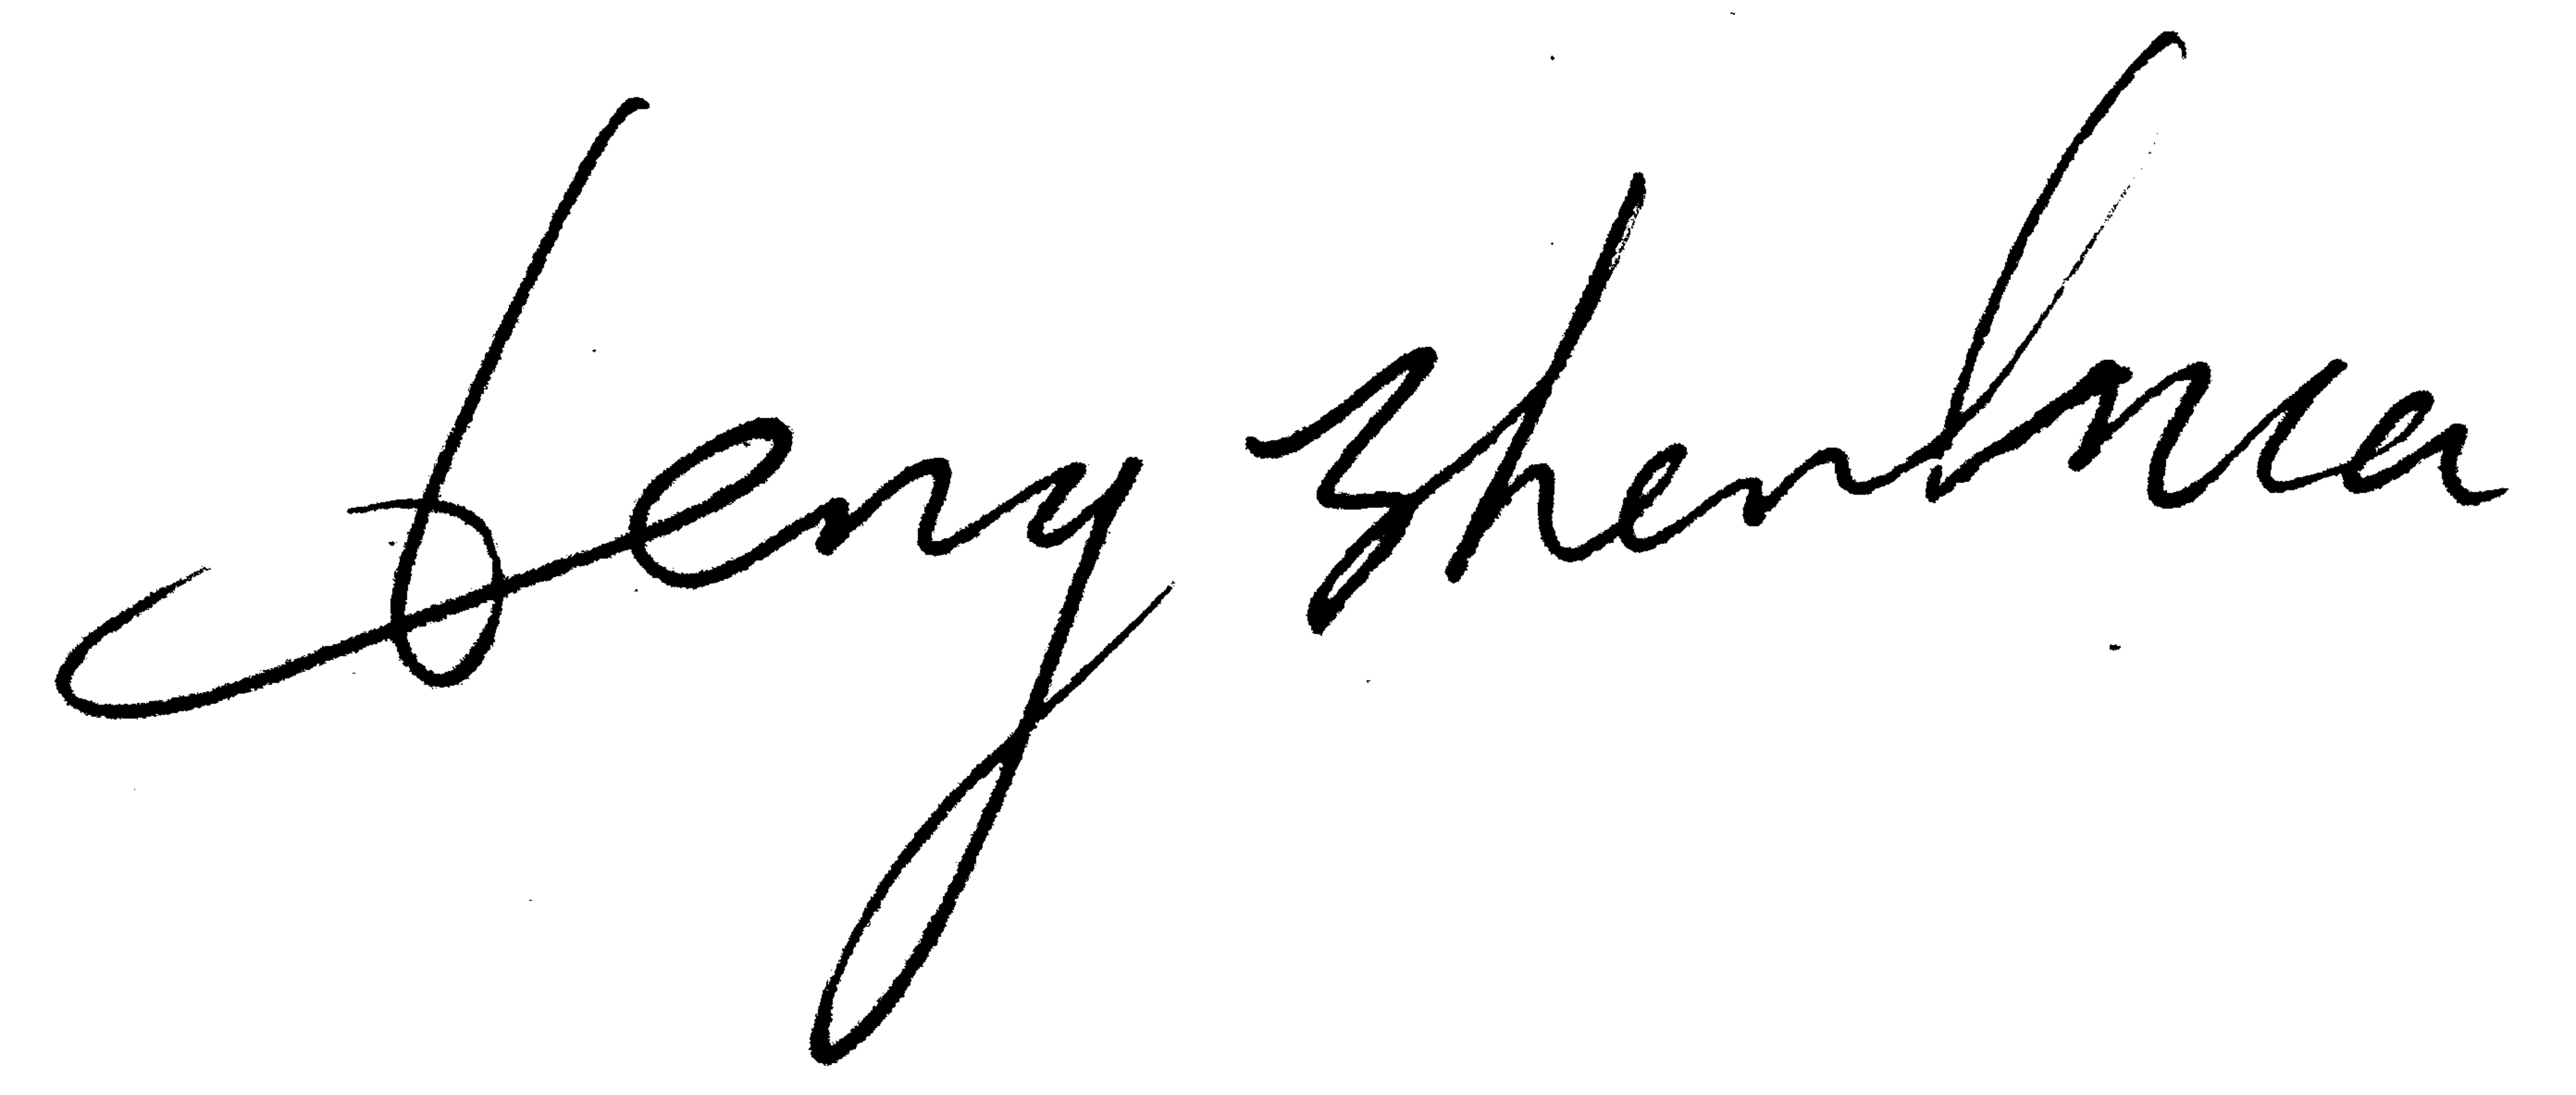
\includegraphics[width=3cm]{英文签名.pdf}}\\
%\rightline{2016年12月22日}
\rightline{2018年9月1日}

%\tableofcontents
  \chapter{运动的描述}
  \section{运动学基本概念}
\subsubsection{质点}

在研究物体的机械运动时,为简化问题可以抓住主要问题忽略次要问题做一定的简化.如果在所研究的问题中,物体的\CJKunderwave{大小和形状对该问题影响不大}时,则可以忽略物体的大小,将物体看成一个有质量的几何点,叫做质点.

质点是一种\CJKunderwave{理想物理模型},它实际上不存在,由于问题的复杂性往往采用一定的近似使它简化.比如,点电荷也是一种理想模型,还有理想变压器等.

\begin{selection}
  s1.下列关于质点的说法中,正确的是[D]
  A.质点是一个理想化的模型,实际上并不存在,所以引入这个概念没有多大意义
  B.体积很小的物体更容易看做质点
  C.凡轻小的物体,皆可看做质点
  D.当物体的形状和大小对所研究的问题属于无关或者次要因素时,即可把物体看成质点

  a.*

  e.建立理想模型是物理中的重要的研究方法,对于复杂问题的研究有重大意义,A错误;一个物体能否看做质点不应看其大小,关键是看其大小对于研究的问题的影响能否忽略,体积很小的物体有时可以看成质点,有时不能看成质点,B错误;一个物体能否看成质点不以轻重而论,C错误;物体能否看成质点取决于其大小和形状对所研究的问题是否属于无关或次要因素,若是就可以看成质点,D正确.

\end{selection}
\subsubsection{参考系}
要描述一个物体的运动,首先要选定某个其它的物体做参考,观察物体相对于这个``其它物体''的位置是否随时间变化,以及怎样变化.这种 \CJKunderwave{用来做参考的物体} 称为参考系.

对一个物体的运动情况的描述,取决于所选择的参考系,选取的参考系不同,对于同一个物体运动的描述一般也不相同.

参考系具有相对性.它的具体含意为:对于一个物体的运动, \CJKunderwave{总能够找到一个参考系,使该物体对于此参考系是静止的} ,也就是静止具有相对性.对于多个物体,一般它们的运动不相同, \CJKunderwave{找不到一个参考系,使所有的物体对于该参考系都静止} ,也就是运动具有绝对性.

\begin{selection}
  s1.关于参考系,下列说法正确的是[D]
  A.参考系必须是静止不动的物体
  B.参考系必须是静止不动或正在做直线运动的物体
  C.研究物体的运动,可选择不同的参考系,但是选择不同的参考系观察的结果是一样的
  D.研究物体的运动,可选择不同的参考系,但选择不同的参考系研究同一物体的运动而言,一般会出现不同的结果

  a.*

  e.参考系的选取是任意的,A,B错误;选择不同的参考系,对同一物体运动的描述一般是不同的,C错误,D正确.

\end{selection}

\subsubsection{坐标系}
上一节中,参考系可以确定物体是静还是动的问题.但是不能确定动多么快的问题,也就是定性的,所以要准确的描述物体的位置及位置变化需要建立坐标系,这个坐标系包括:\CJKunderwave{原点,正方向和单位长度.}

研究物体的直线运动时,一般建立直线坐标系,研究物体的曲线运动(轨迹是曲线的运动)时建立平面直角坐标系.另外还有极坐标系,自然坐标系等.感兴趣的同学可以参考一下相关的数学资料.\CJKunderwave{所有坐标系中的一个点和物体的位置一一对应}.

\begin{calculate}
c1.一质点在x轴上运动,各个时刻的位置坐标如
<:
\begin{tabular}{|*{7}{c|}}
  \hline
  t/s & 0 & 1 & 2 & 3 & 4 & 5\\
  \hline
  x/m & 0 & 5 & -4 & -1 & -7 & 1\\
  \hline
\end{tabular}
:>所示:
[1]请画出x轴,在上面标出质点在各个时刻的位置.
[2]哪个时刻离开坐标原点最远?有多远?

a.见解析

e.(1)各时刻质点的位置坐标如
<:
{\tiny	
  \begin{tikzpicture}[scale=0.4]
    \draw [->] (-8,0)--(7,0);
    \foreach \x in {-7,-6,-5,-4,-3,-2,-1,0,1,2,3,4,5}
    \draw (\x,0pt)--(\x,3pt) node [anchor=north] {\x};
    \draw (8,0) node [anchor=north east] {$x/m$};
    \draw [<-] (-7,4pt)--(-7,24pt) node [anchor=south]{ 4s 末};
    \draw [<-] (-4,4pt)--(-4,24pt) node [anchor=south]{ 2s 末};
    \draw [<-] (-1,4pt)--(-1,24pt) node [anchor=south]{ 3s 末};
    \draw [<-] (1,4pt)--(1,24pt) node [anchor=south]{ 5s 末};
    \draw [<-] (5,4pt)--(5,24pt) node [anchor=south]{ 1s 末};
    \draw [<-] (0,4pt)--(0,44pt) node [anchor=south]{0时刻};
  \end{tikzpicture}
}
:>所示.
\newline
(2)由图可知第4s 末质点离开坐标原点最远,有7m.


\end{calculate}

\subsubsection{时刻}

时刻指的是\CJKunderwave{某一瞬间},在时间轴上\CJKunderwave{时刻用点表示}.

\subsubsection{时间间隔}

时间间隔指某两个时刻之间的间隔,在时间轴上用\CJKunderwave{线段}来表示.

\begin{selection}
  s1.以下计时数据指时间间隔的是[B]
  A.天津开往德州的 k625 次列车于13 点35分从天津发车
  B.李明用15s跑完100米
  C.2013年6月11日下午17时38分,``神舟十号'' 飞船成功发射
  D.某场足球开赛15分钟时甲队攻入一球

  a.B

  e. 列车发车、飞船发射、入球都是事件发生的瞬间,对应的都是时刻,A、C、D错误;跑完100m 是事件发生的过程,对应的是时间间隔,B正确。

\end{selection}

\subsubsection{矢量和标量}
在物理学中,根据不同的物理量的性质可以分为两类:一类\CJKunderwave{既有大小又有方向},同时运算满足\CJKunderwave{平行四边形定则}的称为矢量;另一类是\CJKunderwave{只有大小没有方向},其运算遵守\CJKunderwave{代数运算},称为标量.

平行四边形定则如下:

\begin{figure}[H]
  \centering
  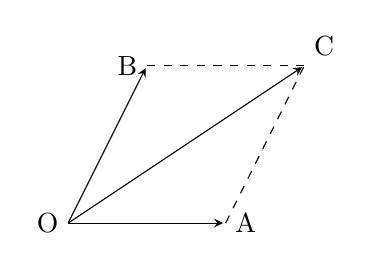
\begin{tikzpicture}
    \draw [->,>=stealth,shorten >=1pt] (0,0)--(2,0) node [anchor=west]{A};
    \draw [->,>=stealth,shorten >=1pt] (0,0)--(1,2) node [anchor=east]{B};
    \draw [dashed] (1,2) --(3,2);
    \draw [dashed] (2,0)--(3,2);
    \draw [->,>=stealth,shorten >=1pt] (0,0)--(3,2) node [anchor=south west]{C};
    \draw (0,0) node [anchor=east]{O};
  \end{tikzpicture}
  \caption{平行四边形定则}
  \label{fig:parallelogram law}
\end{figure}

$$\vec{C}=\vec{A}+\vec{B}$$

数学上舍弃矢量的实际含义,就抽象为数学中的概念---向量.同学们要掌握向量的计算方法,如果不熟悉的话,请参考数学书籍先补充上这一部分知识.

\subsubsection{路程}

路程指\CJKunderwave{物体运动轨迹的长度},是一个\CJKunderwave{标量}.

\subsubsection{位移}

位移指从\CJKunderwave{初位置}到\CJKunderwave{末位置}的有向线段,是一个矢量,大小就是该有向线段的长度,方向就是前头所指的方向.

描述一个物体的机械运动,准确的应该使用位移.但是同学们在读初中的时候使用路程来计算,并没有遇到错误,那是因为在初中研究的都是单向直线运动,\CJKunderwave{单向直线运动中位移的大小与路程相等},同时只有一个方向,所以在计算过程中略去方向的考虑并不会导致问题.

\begin{figure}[H]
  \centering
  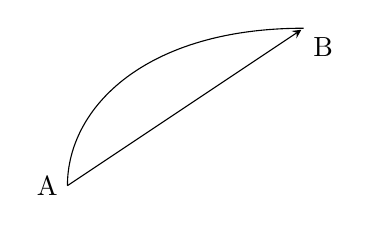
\begin{tikzpicture}
    \draw (0,0) .. controls (0,1) and (1,2) .. (3,2);
    \draw [->,>=stealth,shorten >=1pt] (0,0) -- (3,2);
    \draw (0,0) node [anchor=east]{A};
    \draw (3,2) node [anchor=north west]{B};
  \end{tikzpicture}
  \caption{位移}
  \label{fig:displacement}
\end{figure}

如图\ref{fig:displacement}所示,由A到B的位移记为$\overrightarrow{AB}$,但是路程由两个不同的路径是不同的.同时也能看到,对于\CJKunderwave{曲线运动它的位移大小小于路程},但是单向直线运动中它们是相等的.

对于直线运动的位移可以用$x_1$表示质点的起始位置,$x_2$表示质点的末位置,则以$\Delta x=x_2-x_1$表示位移.
如果$\Delta x>0$表示位移方向向右,如果$\Delta x<0$表示位移方向向左.

\begin{figure}[H]
  \centering
    \begin{tikzpicture}
      \draw [->] (0,0)--(3,0) node [anchor=north] {\small $x/m$};
      \draw (1,0)--(1,4pt) node [anchor=south] {\small $x_1$};
      \draw (2,0)--(2,4pt) node [anchor=south] {\small $x_2$};
    \end{tikzpicture}
  \caption{直线运动的位移}
\end{figure}

  \begin{selection}
    s1.下列关于位移(矢量)和温度(标量)的说法中,正确的是[D]
    A.两个运动物体的位移大小均为$30m$,则这两个位移一定相同
    B.做直线运动的两个物体的位移$x_1=3m$, $x_2=-5m$,则$x_1>x_2$
    C.温度计计数有正也有负,其正,负号表示方向
    D.温度计计数的正负号表示温度的高低,不能表示方向

    a.*

    e.两个矢量相同指矢量的大小和方向两个要素都相同,所以A由于可能方向不同,所以错;直线运动的位移的``$+$''表示与正方向相同,``$-$''表示与正方向相反;温度是标量,标量的正负号表示大小(也就是温度的高低).

    s2.(多选)关于位移和路程,下列说法正确的是[BCD]
    A.在某一段时间内物体运动的位移为零,则该物体一定是静止的
    B.在某一段时间内物体运动的路程为零,则该物体一定是静止的.
    C.在直线运动中,物体的位移大小可能等于其路程
    D.在曲线运动中,物体的位移大小一定小于其路程

    a.BCD

    e.位移为零,表明该物体在运动过程中的初、末位置相同,物体不一定静止,A项错误;路程为零,表明运动轨迹的长度为零,物体一定静止,B项正确;当物体做单向直线运动时,其位移大小等于路程,C项正确;物体在做曲线运动时,初、末位置直线距离小于轨迹长度,所以位移大小一定小于路程,D项正确.

    s3.(多选)对位移和路程理解正确的是[BC]
    A.路程是个标量,是由初始位置指向终止位置的有向线段
    B.位移是个矢量,是由初始位置指向终止位置的有向线段
    C.路程是物体实际运动轨迹的长度,它没有方向
    D.当物体做直线运动时,位移和路程是相同的物理量

    a.BC

    e.路程是物体实际运动轨迹的长度,是标量;位移是由初始位置指向终止位置的有向线段,是矢量.当物体做单向直线运动时,两者大小相等,但不相同.综上,选项B,C正确.

  \end{selection}
  \begin{calculate}
   c1.如
   <:
   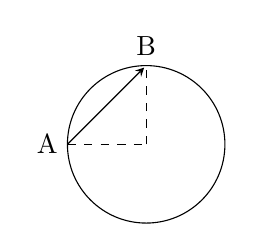
\begin{tikzpicture}
     \draw (0,0) circle [radius=1];
     \draw [->,>=stealth,shorten >=1pt] (-1,0) --(0,1);
     \draw (-1,0) node [anchor=east]{A};
     \draw (0,1) node [anchor=south]{B};
     \draw [dashed] (0,0) --(0,1);
     \draw [dashed] (-1,0)--(0,0);
   \end{tikzpicture}
   :>
   所示,一质点沿半径为$20cm$ 的圆周自A 点出发,逆时针运动$\cfrac{3}{4}$圆周到达B点.求质点的位移和路程.

a. 位移大小为$28.3cm$,方向自A点指向B点,路程为$94.2cm$

e.如图,位移大小为AB线段的长度
$$AB=\sqrt{2}r\approx28.3cm$$
方向:由A点指向B点
\newline
路程为
$$s=\cfrac{3}{4}\cdot2\pi r=94.2cm$$

c2.一个袋子里有$40kg$ 大米,再放入$30kg$大米,袋子中大米的质量是多少?如果一位同学从操场中心A点出发向北走了$40m$ 到达B点,然后又向西走了$30m$ 到达C点,则他从A点到C点的路程是多大?位移是多少?从大小的计算方法上看,质量、路程和位移有什么不同?

a.见解析

e.袋子中大米的质量是$40kg+30kg=70kg$.如
<:
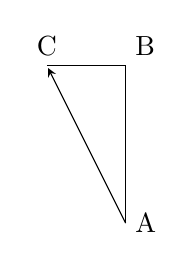
\begin{tikzpicture}
  \draw [->,>=stealth,shorten >=1pt] (0,0)--(-1,2) node [anchor=south]{C};
  \draw (0,0) -- (0,2) node [anchor=south west]{B};
  \draw (-1,2)--(0,2);
  \draw (0,0) node [anchor=west]{A};
\end{tikzpicture}
:>所示,路程是$40m+30m=70m$,位移从A点指向C点的有向线段,大小为$AC=50m$.质量,路程是标量,遵从算术加减法的法则,可以直接相加减;位移是矢量,不能直接相加减,位移的大小等于初位置指向末位置的有向线段的长度.

  \end{calculate}


  \newpage
  \section{速度和速率}
\subsection{机械运动}
物体的位置随时间的变化,我们称之为机械运动.简言之,就是研究物体的位移随时间的变化.
\subsection{速度}
\subsubsection{定义}
质点在$\Delta t$ 时间内发生的位移$ \Delta x $ 与 时间的比值,定义为速度.用公式表达如下
\begin{equation}
  v=\cfrac{\Delta x}{\Delta t}\label{eq:velocity}
\end{equation}
\subsubsection{矢标性}
 从定义上来看,位移$\Delta x$ 是一个矢量,时间$\Delta t$ 是一个标量,矢量除以标量还是一个矢量.所以速度是一个矢量.速度的方向我们称之为质点运动的方向,在一些题目中没有明确提出,也这样认为.
 \subsubsection{单位}
 每一个物理量都有一个特定的意义,所以也必然有一个单位.从定义看来,位移的单位是``米'',时间的单位是``秒'',所以速度单位是:米/秒,符号为$m/s$
\subsubsection{速度的物理意义}
速度是表征物体运动快慢的物理量.这里大家注意,如果问某个物理量的物理意义,我们统一的说法是:XX是表征XXXX的物理量.
\subsection{瞬时速度和平均速度}
\subsubsection{瞬时速度}
瞬时速度描述物理某一瞬时的运动的快慢,所以要求时间$\Delta t \rightarrow 0$,瞬时速度的定义为:
\begin{equation}
 v=\lim_{\Delta t \to 0} \cfrac{\Delta x}{\Delta t}
  \label{eq:instantaneous velocity}
\end{equation}

\subsubsection{平均速度}
平均速度描述质点运动的平均快慢程度,所以是在一段时间内发生的,不要求时间趋于零.为了区别于瞬时速度,在速度$v$ 的上方加一个横杠$\overline{v}$,读作 ``维拔'',其定义为:
\begin{equation}
\overline{v}=\cfrac{\Delta x}{\Delta t}
  \label{eq:average velocity}
\end{equation}

\subsection{速率}
\subsubsection{定义}
速率是指路程比上时间,表示单位时间内发生的路程.定义如下
\begin{equation}
v=\cfrac{\Delta s}{\Delta t}
  \label{eq:speed}
\end{equation}

\subsubsection{矢标性}
从速率的定义来看,路程是标量,时间是标量,所以速率也是一个标量.

\subsubsection{单位}
从速率定义来看,速率的单位和速度相同,都是$m/s$



\subsubsection{瞬时速率}
类比速度,则速率也分为瞬时速率和平均速率,瞬时速率定义如下:
\begin{equation}
v=\lim_{\Delta t \to 0} \cfrac{\Delta s}{\Delta t}
  \label{eq:instantaneous speed}
\end{equation}

\subsubsection{平均速率}
类比速度,则速率也分为瞬时速率和平均速率,平均速率定义如下:
\begin{equation}
\overline{v}=\cfrac{\Delta s}{\Delta t}
  \label{eq:average speed}
\end{equation}

\subsubsection{注意事项}
在初中时同学们运算都采用的速率,但是当时没有区分速度和速率,因为当时研究的是单向直线运动,这种情况下速度的大小和速率是相等的,所以没有出现错误.然而一旦情况复杂,则必须用速度来描述.

今后如没有特殊声明,则一律使用速度来描述运动,不再使用速率.

\subsection{例题分析}
\begin{selection}
  1.关于速度的定义$v=\frac{\Delta x}{\Delta t}$ ,以下叙述正确的是
  A.物体做匀速直线运动时,速度$v$ 与运动的位移 $\Delta x$ 成正比,与运动时间$\Delta t$ 成反比
  B.速度$v$ 的大小与运动的位移$\Delta x$ 和时间$\Delta t$ 都无关
  C.此速度定义适用于任何运动
  D.速度是表示物体运动快慢及方向的物理量

  a.BCD

  e.$v=\frac{\Delta v}{\Delta t}$ 是速度的定义式,所以适用于一切情况,C对;此定义法为比值定义法,不能说此物理量与分子成正比或者与分母成反比,所以A错,B对;速度的大小表示运动的快慢,方向表示物体运动的方向,所以D对.

  2.物体沿直线做单向直线运动,途经直线上的A,B,C 三点,经过这三点时的速度分别为$v_A$ , $v_B$ , $v_C$ ,则下列说法正确的是
  A.$v_A$, $v_B$ , $v_C$ 越大,则由A到C所用的时间越短
  B.经过 A,B,C 三点时的瞬时速率就是$v_A$ , $v_B$ , $v_C$
  C.由A到C这一阶段的平均速度为$\overline{v}=\frac{v_A+v_B+v_C}{3}$
  D.由A到C这一阶段的平均速度越大,则由A到C所用的时间越短

  a.D

  e.A到C所用时间取决于A到C的平均速度,与初,末态的瞬时速度无关,A错误,D正确.瞬时速度的大小叫瞬时速率,B错误.平均速度一般不等于速度的平均值,C错误.

\end{selection}

\begin{calculate}
3.一辆汽车由A出发做直线运动,前$5s$ 向东行驶了$30m$ 到达 B 点,又行驶了$5s$ 前进了$60m$ 到达 C点,在C点停了$4s$ 后又向西行驶,经历了$6s$  运动$12m$ 到达 A点西侧的D点.求
[1]全过程的平均速度;
[2]全过程的平均速率.

a.(1)平均速度大小为$1.5m/s$,方向水平向西 (2) 平均速率为$10.5m/s$

e.(1)设向东为正方向
$$x=30m+60m+(-120m)=-30m$$
全程用时
$$t=5s+5s+4s+6s=20s$$
所以平均速度为
$$\overline{v}=\cfrac{x}{t}=\cfrac{-30m}{20s}=-1.5m/s$$
负号表示速度方向向西
\newline
(2)全程的路程为
$$s=30m+60m+120m=210m$$
所以平均速率为
$$\overline{v}=\cfrac{s}{t}=\cfrac{210m}{20s}=10.5m/s$$


\end{calculate}

  \newpage
  \section{加速度}
在描述物体的机械运动时,我们不仅要知道某一时刻物体在哪里(位移),向哪个方向运动的快慢(速度),而且也需要知道\CJKunderwave{物体速度变化的快慢},所以引入加速度.

\subsection{加速度}
\subsubsection{定义}
加速度定义为\CJKunderwave{速度的变化量}和\CJKunderwave{时间}的比值,如下
\begin{equation}
  a=\cfrac{\Delta v}{\Delta t} \label{eq:acceleration}
\end{equation}

\subsubsection{物理意义}
\CJKunderwave{加速度}是表征物体\CJKunderwave{速度变化快慢}的物理量.

\subsubsection{矢标性}
从定义上来看,速度的变化量$\Delta v$ 是矢量,时间 $\Delta t$ 是标量,所以加速度也是一个\CJKunderwave{矢量}.它的方向与\CJKunderwave{速度变化量}$\Delta v$ 的方向一致.
\subsubsection{单位}
从定义上来看,速度变化量的单位是$m/s$,时间的单位是$s$ ,所以加速度的单位是:\CJKunderwave{ 米每二次方秒},记作$m/s^2$

\subsection{瞬时加速度和平均加速度}
类比瞬时速度和平均速度,加速度也有瞬时加速度和平均加速度.

\subsubsection{瞬时加速度}
瞬时加速度用来描述某\CJKunderwave{一个时刻}速度变化的快慢.其定义如下:
\begin{equation}
a=\lim_{\Delta t \to 0} \cfrac{\Delta v}{\Delta t}
  \label{eq:instantaneous acceleration}
\end{equation}

\subsubsection{平均加速度}
平均加速度用来描述某\CJKunderwave{一段时间}内速度平均变化快慢.其定义如下:
\begin{equation}
\overline{a} =\cfrac{\Delta v }{\Delta t}
  \label{eq:average acceleration}
\end{equation}

\subsection{加速与减速的判断}

在具体的运动中,物体有可能加速也有可能减速,但是没有{\bf 减速度}一词.所有变速运动速度的变化量与
时间的比值都叫加速度,这只是一个名称而已.

如果物体运动的轨迹是直线,则称为直线运动,在直线运动中,如果 $v$ 与 $a$ 方向相同则加速,如果 $v$ 与 $a$ 的方向相反则减速.

如果物体运动的轨迹是曲线,则称为曲线运动,在曲线运动中,如果 $v$ 与 $a$ 的夹角是锐角则加速,如果 $v$ 与 $a$ 夹角为钝角则减速,如果 $v$ 与 $a$ 的夹角是直角,则速度大小不发生变化,只有速度的方向发生变化.

\subsection{注意事项}
在物理学中经常用比值定义法来定义物理量,这就好比用钱来定义钱包一样:\CJKunderwave{钱包是用来盛钱的包}.但是钱包和钱的多少没关系.所以加速度$a$ 和 $\Delta v$也没有关系,与$\Delta t$也没有关系,它\CJKunderwave{只取决于速度变化量和时间的比值}.

$\Delta$这个符号用来表示\CJKunderwave{一个末态的量减去一个初态的量},比如:$\Delta v =v_2 -v_1$,其中$v_1$是初始的速度,$v_2$是末速度.以后遇到的所有$\Delta$都具备此含义.

按上面的表述,则$\Delta t >0$是\CJKunderwave{永远成立}的.所以$a$与$\Delta v$的符号相同,因此说加速度的方向与速度变化量的方向一致.

\subsection{例题分析}
\begin{selection}
  1.一辆汽车正在公路上行驶,关于汽车的运动,下列说法正确的是
  A.汽车的速度改变量越大,加速度一定越大
  B.速度很大的汽车,其加速度可能很小,但不能为零
  C.某时刻汽车的速度为零,其加速度可能很大
  D.汽车加速度很大时,其速度一定很大

  a.C

  e.汽车的速度改变量越大,加速度不一定越大,因为加速度与速度改变量和时间间隔两个因素有关,选项A错误;速度很大的汽车,加速度可能很小,也可能为零,例如匀速直线运动的汽车,选项B 错误;汽车速度为零时,加速度可能很大,例如汽车刚启动时,选项C正确,D错误.

  2.由加速度的定义式$a=\cfrac{\Delta v}{\Delta t}$可知
  A.加速度$a$与速度的变化$\Delta v$ 成正比
  B.加速度$a$ 大小由速度变化$\Delta v$ 决定
  C.加速度$a$ 的方向与速度$v$ 的方向 相同
  D.加速度$a$ 的方向与$\Delta v$的方向相同

  a.D

  e.$a=\cfrac{\Delta v}{\Delta t} $ 是加速度的定义式,是比值定义法,不能说加速度与分子和分母单独有关,所以A,B 错误.由于$\Delta t>0$ 永远成立,所以 $a$ 的符号与$\Delta v$ 的正负号相同,一个矢量正负号表示方向,所以D 正确.

  3.某物体沿直线运动,其$v-t$ 图象如
  <:
  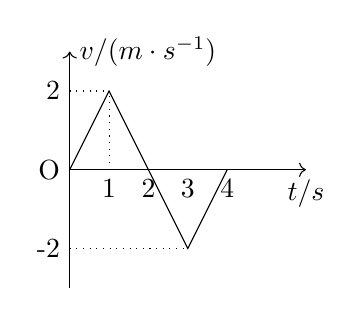
\begin{tikzpicture}
    \draw[->] (0,0)--(3,0) node [anchor=north ]{$t/s$};
    \draw[->] (0,-1.5)--(0,1.5) node [anchor=west]{$v/(m\cdot s^{-1})$};
    \draw (0,0) node [anchor=east] {O};
    \draw (0.5,0) node [anchor=north]{1};
    \draw (1,0) node [anchor=north]{2};
    \draw (1.5,0) node [anchor=north]{3};
    \draw (2,0) node [anchor=north]{4};
    \draw (0,0)--(0.5,1)--(1.5,-1)--(2,0);
    \draw [dotted](0,1)node [anchor=east]{2}--(0.5,1);
    \draw [dotted] (0.5,0)--(0.5,1);
    \draw [dotted](0,-1)node [anchor=east]{-2}--(1.5,-1);
  \end{tikzpicture}
  :>所示,下列说法正确的是
  A.第$1s$ 内和 第$2s$ 内物体的速度方向相反
  B.第$1s$ 内和第$2s$ 内物体的加速度方向相反
  C.第$3s$ 内物体的速度方向和加速度方向相反
  D.第$2s$ 末物体的加速度为零

  a.B

  e.速度的方向由纵坐标的正负表示,正号表示与正方向相同,负号表示与正方向相反.加速度的方向由$v-t$ 图象的斜率的正负表示,正号表示加速度沿正方向,负号表示加速度沿负方向.第$1s$ 内,第$2s$ 内纵坐标为正,速度均为正向,A错误;根据斜率的正负,第$1s$ 内加速度为正向,第$2s$ 内加速度为负方向,B正确;第$3s$ 内速度为负方向,加速度为负方向,C错误;第$2s$ 末物体的加速度为$-2m/s^2$,D错误.

\end{selection}


  %\chapter{匀变速直线运动}
\setcounter{chapter}{2}
  \section{匀变速直线运动速度与时间的关系}
\subsection{基本关系推导}
在速度发生变化的运动中,如果加速度保持不变,则称为匀变速直线运动.这是一类最简单的变速运动.

$t=0$时的速度记为$v_0$,$t$时刻的速度记为$v$,则代入加速度的定义\eqref{eq:acceleration}式:
\[
a=\cfrac{v-v_0}{t-0}
\]
上式左右同时乘以时间$t$,再加上$v_0$,移项得
\begin{equation}
  v=v_0+at
  \label{eq:v-t}
\end{equation}

\subsection{例题分析}

\begin{calculate}
  1.A,B是做匀变速直线运动的两个物体的速度时间图象,如
<:
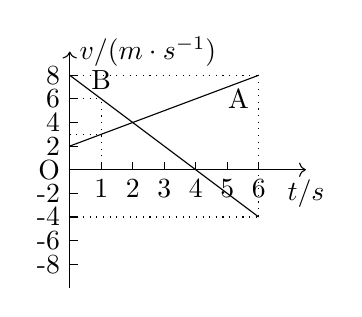
\begin{tikzpicture}
  \draw [->](0,0)--(3,0) node [anchor=north]{$t/s$};
  \draw [->](0,-1.5)--(0,1.5) node [anchor=west]{$v/(m\cdot s^{-1})$};
  \draw (0,0) node [anchor=east] {O};
  \draw (0.4,0.1)--(0.4,0) node [anchor=north] {1};
  \draw (0.8,0.1)--(0.8,0) node [anchor=north] {2};
  \draw (1.2,0.1)--(1.2,0) node [anchor=north] {3};
  \draw (1.6,0.1)--(1.6,0) node [anchor=north] {4};
  \draw (2.0,0.1)--(2.0,0) node [anchor=north] {5};
  \draw (2.4,0.1)--(2.4,0) node [anchor=north] {6};
  \draw (0.1,0.3)--(0,0.3) node [anchor=east]{2};
  \draw (0.1,0.6)--(0,0.6) node [anchor=east]{4};
  \draw (0.1,0.9)--(0,0.9) node [anchor=east]{6};
  \draw (0.1,1.2)--(0,1.2) node [anchor=east]{8};
  \draw (0.1,-0.3)--(0,-0.3) node [anchor=east]{-2};
  \draw (0.1,-0.6)--(0,-0.6) node [anchor=east]{-4};
  \draw (0.1,-0.9)--(0,-0.9) node [anchor=east]{-6};
  \draw (0.1,-1.2)--(0,-1.2) node [anchor=east]{-8};
  \draw (0,0.3) --(2.4,1.2);
  \draw (0,1.2) --(2.4,-0.6);
  \draw [dotted] (0,1.2)--(2.4,1.2);
  \draw [dotted] (0,-0.6)--(2.4,-0.6);
  \draw [dotted] (2.4,1.2)--(2.4,-0.6);
  \draw [dotted] (0.4,0)--(0.4,0.9);
  \draw[dotted] (0,0.9)--(0.4,0.9);
  \draw[dotted] (0,0.45)--(0.4,0.45);
  \draw (0.4,0.9) node [anchor=south]{B};
  \draw (2.4,0.9) node [anchor=east]{A};
\end{tikzpicture}
:>
[1]A,B各做什么运动并求其加速度;
[2]两图象交点的意义;
[3]求$1s$ A,B的速度;
[4]求$6s$ 末A,B的速度.
  
a.见解析

e.(1) A物体沿规定的正方向做匀加速直线运动,加速度大小为 $a_1=\frac{v-v_0}{t}=\frac{8-2}{6}m/s^2=1m/s^2$ ,方向与初速度方向相同;B物体前$4s$沿规定的正方向做匀减速直线运动,$4s$ 后沿反方向做匀加速直线运动,加速度为$a_2=\frac{0-8}{4}m/s^2=-2m/s^2$ ,负号表示加速度方向与初速度方向相反.
\newline
(2)两图象的交点表示在该时刻A,B速度相同.
\newline
(3)$1s$末A物体的速度为$3m/s$,和初速度方向相同;B物体的速度为$6m/s$ ,和初速度方向相同.
\newline
(4)$6s$ 末A物体的速度为$8m/s$ ,和初速度方向相同;B物体的速度为$-4m/s$,和初速度方向相反.

2.一物体从静止开始以$2m/s^2$ 的加速度做匀加速直线运动,经过$5s$ 后做匀速直线运动,最后$2s$ 的时间内物体做匀减速直线运动直到静止.求
[1]物体做匀加速直线运动时速度大小;
[2]物体做匀减速直线运动时的加速度.

a.(1) $10m/s$ (2) $-5m/s^2$ ,加速度方向与$v_c$ 方向相反.

e.此题先画出草图如
<:
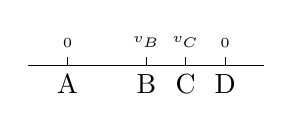
\begin{tikzpicture}
 \draw (0,0)--(3,0);
 \draw (0.5,0)node[anchor=north]{A}--(0.5,0.1) node [anchor=south] {\tiny $0$};
 \draw (1.5,0)node[anchor=north]{B}--(1.5,0.1) node [anchor=south] {\tiny $v_B$};
 \draw (2,0)node[anchor=north]{C}--(2,0.1) node [anchor=south] {\tiny $v_C$};
 \draw (2.5,0)node[anchor=north]{D}--(2.5,0.1) node [anchor=south] {\tiny $0$};
\end{tikzpicture}
:>
所示,设图中$A\rightarrow B$ 为匀加速直线运动,$B \rightarrow C$为匀速直线运动,$C\rightarrow D$为匀减速直线运动,$BC$段的速度为$AB$段的末速度,也是$CD$ 段的初速度.
\newline
(1)由速度与时间的关系\eqref{eq:v-t}式得
$$v_B=a_1t_1=2\times 5 m/s=10m/s$$
即做匀速直线运动的速度为$10m/s$
\newline
(2)由加速度的定义\eqref{eq:acceleration}式得
$$a_2=\cfrac{v-v_0}{t_2}=\cfrac{v_D-v_C}{t_2}=\cfrac{0-10}{2}m/s^2=-5m/s^2$$
负号表示加速度方向与$v_C$方向相反.

\end{calculate}

  \section{匀速直线运动位移与时间的关系}

为了导出匀变速直线运动位移与时间的关系先来推导一下最简单的匀速直线运动的位移与时间的关系.所谓匀速直线运动,指速度保持不变的运动,即:速度大小和方向都不发生变化.

记$t=0$时的位移为零,t时刻的位移为$x$,代入速度的定义式\eqref{eq:velocity}式:

\begin{equation*}
v=\cfrac{x-0}{t-0}
\end{equation*}

将上式左右同时乘以时间$t$,然后再移项得:

\begin{equation}
  x=vt
  \label{eq:uniform displacement}
\end{equation}

匀速直线运动的$v-t$图象为:

\begin{figure}[H]
  \centering
  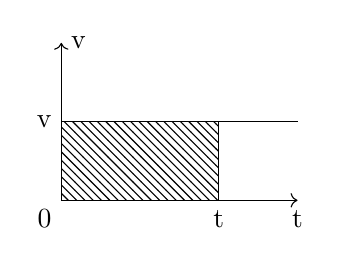
\begin{tikzpicture}
    \draw [->] (0,0) -- (3,0) node [anchor= north]{t};
    \draw [->] (0,0) -- (0,2) node [anchor= west]{v};
    \draw (0,1)--(3,1);
    \draw [pattern=north west lines](0,0) rectangle (2,1);
    \draw(0,1) node [anchor=east]{v};
    \draw(2,0) node [anchor=north]{t};
    \draw(0,0) node [anchor=north east]{0};
  \end{tikzpicture}
  \caption{匀速直线运动$v-t$关系}
  \label{fig:uniform x-t}
\end{figure}

在上图中,显然阴影的面积为$vt$,对比匀速直线运动的位移公式,这个面积正好等于位移.这个结论拓展到匀变速直线运动中也是成立的.

\section{匀变速直线运动位移与时间的关系}

\subsection{基本关系推导}

匀变速直线运动速度是变化的,我们可以利用微元法来求出它的位移.所谓微元法就是按时间分成若干个部分,在每一小段时间内速度变化不大,可以近似认为这一小段内质点做匀速直线运动,然后求出这一小段位移来,同理可以求出每一小段的位移,再将每一小段位移加起来就等于匀变速直线运动的位移了.

如图\ref{fig:weiyuan} 画出匀变速直线运动的速度--时间图象
\begin{figure}[H]
  \centering
\begin{tikzpicture}
  \draw [->] (1,0)--(5,0) node [anchor=north]{t};
  \draw [->] (1,0) -- (1,2.5) node [anchor= west]{$v$};
  \draw(1,0) node [anchor=north east]{0};
  \draw (1,0.5)--(4.4,2.2) node [anchor=south]{$v=v_0+at$};
  \draw (1,0)--(1,0.5);
  \draw (2,0)--(2,1);
  \draw (3,0)--(3,1.5);
  \draw (4,0)--(4,2);
  \draw [pattern=north west lines](1,0) rectangle (2,0.5);
  \draw [pattern=north west lines](2,0) rectangle (3,1);
  \draw [pattern=north west lines](3,0) rectangle (4,1.5);
  \draw (3,-0.5) node [anchor=north] {图:甲};
\end{tikzpicture}
\begin{tikzpicture}
  \draw [->] (1,0)--(5,0) node [anchor=north]{t};
  \draw [->] (1,0) -- (1,2.5) node [anchor= west]{$v$};
  \draw(1,0) node [anchor=north east]{0};
  \draw (1,0.5)--(4.4,2.2) node [anchor=south]{$v=v_0+at$};
  \draw (1,0)--(1,0.5);
  \draw (1.5,0)--(1.5,0.75);
  \draw (2,0)--(2,1);
  \draw (2.5,0)--(2.5,1.25);
  \draw (3,0)--(3,1.5);
  \draw (3.5,0)--(3.5,1.75);
  \draw (4,0)--(4,2);
  \draw [pattern=north west lines](1,0) rectangle (1.5,0.5);
  \draw [pattern=north west lines](1.5,0) rectangle (2,0.75);
  \draw [pattern=north west lines](2,0) rectangle (2.5,1);
  \draw [pattern=north west lines](2.5,0) rectangle (3,1.25);
  \draw [pattern=north west lines](3,0) rectangle (3.5,1.5);
  \draw [pattern=north west lines](3.5,0) rectangle (4,1.75);
  \draw (3,-0.5) node [anchor=north] {图:乙};
\end{tikzpicture}
  \caption{微元法求位移}
  \label{fig:weiyuan}
\end{figure}

图甲等分时间的间隔较大,图乙等分间隔是甲的一半.无论是甲还是乙,均可以用阴影的小矩形的面积表示一小段时间内的位移,然后加起来就得到近似的匀变速直线运动的位移.但是甲的间隔较乙为大,所以甲不如乙精确,如果对乙再细分下去会得到更加精确的近似位移.可以预见当无限分割时间时,将会得到严格的位移,阴影也就成为了一个梯形,如下

\begin{figure}[H]
  \centering
  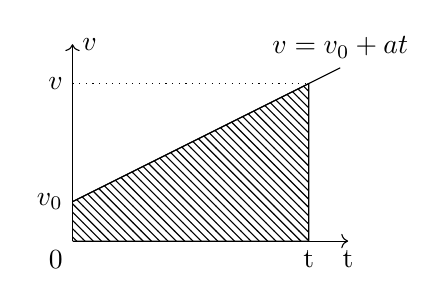
\begin{tikzpicture}
  \draw [->] (1,0)--(4.5,0) node [anchor=north]{t};
  \draw [->] (1,0) -- (1,2.5) node [anchor= west]{$v$};
  \draw(1,0) node [anchor=north east]{0};
  \draw (1,0.5)--(4.4,2.2) node [anchor=south]{$v=v_0+at$};
  \draw [pattern=north west lines](1,0)--(4,0)--(4,2)--(1,0.5);
  \draw (4,0) node [anchor=north]{t};
  \draw (1,2) node [anchor=east]{$v$};
  \draw (1,0.5) node [anchor=east]{$v_0$};
  \draw[dotted] (1,2)--(4,2); 
  \end{tikzpicture}
  \caption{匀变速直线运动$x-t$关系}
  \label{fig:x-t}
\end{figure}

由梯形的面积计算公式易得,匀变速直线运动的位移公式为:
\begin{equation}
x=\cfrac{(v+v_0)t}{2}
  \label{eq:displacement}
\end{equation}

上面这个公式是推导匀变速直线运动的基本关系,一定要记牢.上述公式含有 $t$ 时刻的速度 $v$ ,将 \eqref{eq:v-t} 式代入 \eqref{eq:displacement} 消去 $v$ 便得到:

\begin{equation*}
x=\cfrac{(v_0+at+v_0)t}{2}=v_0t+\cfrac{1}{2}at^2
\end{equation*}

即匀变速直线运动位移与时间的关系为:

\begin{equation}
x=v_0t+\cfrac{1}{2}at^2
  \label{eq:x-t}
\end{equation}

\subsection{例题分析}
\begin{calculate}
  1.一物体做初速度为零的匀加速直线运动,加速度大小为$a=2m/s^2$,求:
  [1] 第$5s$ 末物体的速度多大?
  [2] 前$4s$ 的位移多大?
  [3] 第 $4s$ 内的位移多大?

  a.(1) $10m/s$ (2) $16m$ (3) $7m$

  e.(1)第$5s$ 末物体的速度由 \eqref{eq:v-t} 式得
  $$v_1=0+2\times 5m/s=10m/s$$
  (2)前$4s$ 的位移由\eqref{eq:x-t} 式得
  $$x_1=0+\cfrac{1}{2}\times 2\times 4^2m=16m$$
  (3)物体第3秒末的速度由\eqref{eq:v-t}式得
  $$v_2=v_0+at_2=6m/s$$
  则第$4s$ 内的位移由\eqref{eq:x-t}式得
  $$x_2=v_2t_3+\cfrac{1}{2}at_3^2=7m$$

  2.一辆汽车正在平直的公路上以$72km/h$ 的速度行驶,司机看见红色信号灯便立即踩下制动器,此后,汽车开始做匀减速直线运动.设汽车减速过程的加速度大小为$5m/s$,求:
  [1]开始制动后,前$2s$ 内汽车行驶的距离;
  [2]开始制动后,前$5s$ 内汽车行驶的距离.

  a.(1) $30m$ (2) $40m$

  e.首先将速度的单位换算为国际单位,方法如下:
  $$72km/h=\cfrac{72km}{1h}=\cfrac{72\times 10^3m}{3.6\times 10^3 s}=20m/s$$
  由于汽车最后停下来,则刹车时间记为$t_s$,由\eqref{eq:v-t}式可得
  $$t_s=\cfrac{v-v_0}{a}=\cfrac{0-20m/s}{-5m/s^2}=4s$$
  (1)因为$t_1=2s <t_s$,所以汽车在$2s$ 内一直做匀减速直线运动,并没有停下来.由\eqref{eq:x-t}式得:
  $$x_1=v_0t_1+\cfrac{1}{2}at_1^2=20\times2-\cfrac{1}{2}\times5\times2^2 m=30m$$
  (2)因为$t_2=5s>t_s$,所以汽车在$t_s=4s$ 时已经停止运动,而$4s$ 到$5s$ 一直没有运动,所以位移就是前$4s$的位移.
  \newline
  法一:由\eqref{eq:x-t}式得:
  $$x_2=v_0t_s+\cfrac{1}{2}at_s^2=20\times4-\cfrac{1}{2}\times5\times4^2m=40m$$
  法二:由\eqref{eq:displacement}式得
  $$x_2=\cfrac{(v_0+v)t_s}{2}=\cfrac{(20m/s+0)\times 4s}{2}=40m$$
  注意:此题不止一种解法,这里只是演示\eqref{eq:x-t}式和\eqref{eq:displacement}式的使用方法,在刹车类问题中两个方法比较的话,\eqref{eq:displacement}式要比\eqref{eq:x-t}式计算简单,简单的原因是\eqref{eq:displacement}式不涉及平方运算.但是是后面还可以有多种解法,请同学们注意及时回顾.

\end{calculate}

  \section{匀变速直线运动位移与速度的关系}
\subsection{基本关系推导}

有的时候我们不知道时间,但是知道匀变速直线运动中的$v$和$v_0$,以及加速度$a$,如果要计算位移我们需要先根据$v-t$关系计算出时间,再根据$x-t$关系来求位移,这是一个方法,但是不是最简单的方法.本节将导出$x-v$的关系.

利用\eqref{eq:v-t}式解得时间$t=\cfrac{v-v_0}{a}$,将此时间代入\eqref{eq:displacement}式得:
\begin{equation*}
x=\cfrac{(v+v_0)(v-v_0)}{2a}
\end{equation*}
考虑到平方差公式$(v+v_0)(v-v_0)=v^2-v_0^2$,左右同时乘以$2a$,再移项得:
\begin{equation}
v^2-v_0^2=2ax
  \label{eq:x-v}
\end{equation}
上式就是匀变速直线运动的位移与速度的关系.

\subsection{例题分析}
\begin{calculate}
  1.汽车以$10m/s$ 的速度行驶,刹车的加速度大小为$3m/s^2$ ,求它向前滑行$12.5m$ 后的瞬时速度.

  a.$5m/s$ ,方向与初速度方向相同.

  e.当汽车做刹车运动时,它的速度是不会改变方向的,我们称之为不可逆类问题.设初速度方向为正,则$v_0=10m/s$,$a=-3m/s^2$,$x=12.5m$
  \newline
  法一:由匀变速直线运动位移与速度的关系\eqref{eq:x-v}式得
  $$v=\sqrt{v_0^2+2ax}=\sqrt{10^2+2\times(-3)\times12.5}m/s=5m/s$$
  注意,由于汽车的速度不可能改变方向,所以我们可以判断末速度为正.即汽车向前滑行$12.5m$ 后的瞬时速度大小为$5m/s$,方向与初速度方向相同.
  \newline
  法二:由匀变速直线运动位移与时间的关系\eqref{eq:x-t}式解得
  $$t=\cfrac{-v_0+\sqrt{v_0^2+2ax}}{a}=\cfrac{5}{3}s$$
  再由匀变速直线运动速度与时间的关系\eqref{eq:x-t}式得
  $$v=v_0+at=10+(-3)\times\cfrac{5}{3}m/s=5m/s$$
  \newline
  注意:法一和法二相比更加简单,而法二显然走了弯路.所以在匀变速直线运动问题中,如果根据已知条件选用适当的公式则可以使问题大为简化,所以同学们遇到问题时应当尽量考虑一题多解,从而能够获得选用适当解题方法的能力.

\end{calculate}

\subsubsection{数学补充--求根公式}

在上述题目的第二种解法中用到了一元二次方程的求根公式,依然为了同学们学习的连惯性,这里做详细的证明.如下

一元二次方程为
$$ax^2+bx+c=0$$
上式提出a,并将第二项加入2,变成如下形式
$$a(x^2+2\cfrac{b}{2a}x)+c=0$$
在上式括号内加入$(\cfrac{b}{2a})^2$,然后再减去它则方程不变
$$a(x^2+2\cfrac{b}{2a}x+\cfrac{b^2}{4a^2})+c-\cfrac{b^2}{4a}=0$$
上式中圆括号内为完全平方式,同时将圆括号外的部分移到等号右侧,方程左右同时除以$a$
$$(x+\cfrac{b}{2a})^2=\cfrac{b^2-4ac}{4a^2}$$
记右式分子部分为$\Delta = b^2-4ac$,$\Delta$就是判别式,如果$\Delta <0$则此方程无解,如果$\Delta>0$则对上式开方得
$$x+\cfrac{b}{2a}=\pm \cfrac{\sqrt{\Delta}}{2a}$$
移项得
$$x=\cfrac{-b\pm \sqrt{\Delta}}{2a}$$
上式就是一元二次方程的求根公式.

所以由\eqref{eq:x-t}来求时间时就有:
$$x=v_0t+\cfrac{1}{2}at^2$$
上式移项则相当于关于时间$t$的一元二次方程
$$\cfrac{1}{2}at^2+v_0t-x=0$$
用求根公式解得
$$t=\cfrac{-v_0\pm\sqrt{v_0^2+2ax}}{a}$$
由于时间$t$永远大于零,所以只能取根
$$t=\cfrac{-v_0+\sqrt{v_0^2+2ax}}{a}$$

  \section{匀变速直线运动的推论}
\subsection{平均速度}
平均速度的定义为:
$$\overline{v}=\cfrac{x}{t}$$
将匀变速直线运动的位移\eqref{eq:displacement}式代入平均速度公式可得:
\begin{equation}
\overline{v}=\cfrac{v+v_0}{2}
  \label{eq:average}
\end{equation}

\subsection{中间时刻的瞬时速度}

记中间时刻的瞬时速度为$v_{\frac{t}{2}}$,则由匀变速直线运动速度与时间的关系\eqref{eq:v-t}得:
\begin{align}
v_{\frac{t}{2}}-v_0 &=a\cfrac{t}{2}\\
v-v_{\frac{t}{2}} &=a\cfrac{t}{2}
\end{align}
显然上面二式的右侧相等,所以有
\begin{equation*}
v_{\frac{t}{2}}-v_0=v-v_{\frac{t}{2}}
\end{equation*}
解得:
\begin{equation}
v_{\frac{t}{2}}=\cfrac{(v+v_0)}{2}
  \label{eq:v-half-t}
\end{equation}
对比平均速度公式,此二式可以合写成:
\begin{equation}
\overline{v}=v_{\frac{t}{2}}=\cfrac{(v+v_0)}{2}
  \label{eq:v-average-half}
\end{equation}

\subsection{位移中点的瞬时速度}

位移中点的瞬时速度记为$v_{\frac{x}{2}}$,由匀变速直线运动位移与速度\eqref{eq:x-v}式可得:
\begin{align}
v^2-v_{\frac{x}{2}}^2 &=2a\cfrac{x}{2}\\
v_{\frac{x}{2}}^2-v_0^2 &=2a\cfrac{x}{2}
\end{align}
显然上面二式的右侧相等,所以有
\begin{equation*}
v^2-v_{\frac{x}{2}}^2=v_{\frac{x}{2}}^2-v_0^2
\end{equation*}
解得:
\begin{equation}
v_{\frac{x}{2}}=\sqrt{\cfrac{v^2+v_0^2}{2}}
  \label{eq:v-half-x}
\end{equation}

\subsection{$v_{\frac{t}{2}}$和$v_{\frac{x}{2}}$的大小关系}

\subsubsection{从物理角度证明}

如图\ref{fig:+t-x-middle} 画出了\CJKunderwave{匀加速直线运动}时间中点和位移中点的具体位置.

\begin{figure}[H]
  \centering
  \begin{tikzpicture}
    \draw (0,0) node [anchor=north east]{0}--(4,0) node [anchor=north west]{x};
    \draw (0,0) -- (0,0.25);
    \draw (4,0) -- (4,0.25);
    \draw (1,0) -- (1,0.25) node [anchor=south]{$v_{\frac{t}{2}}$};
    \draw (2,0) -- (2,0.25) node [anchor=south]{$v_{\frac{x}{2}}$};
    \draw (1,0) node [anchor=north]{A};
    \draw (2,0) node [anchor=north]{B};
  \end{tikzpicture}
  \caption{匀加速直线运动}
  \label{fig:+t-x-middle}
\end{figure}

由于图\ref{fig:+t-x-middle} 所示为匀加速直线运动,所以质点从A点到B 点必须\CJKunderwave{加速一段时间},所以可以得到时间中点的瞬时速度 $v_{\frac{t}{2}}$ 小于位移中点的瞬时速度 $v_{\frac{x}{2}}$

如图\ref{fig:-t-x-middle} 画出了\CJKunderwave{匀减速直线运动}时间中点和位移中点的具体位置.

\begin{figure}[H]
  \centering
  \begin{tikzpicture}
    \draw (0,0) node [anchor=north east]{0}--(4,0) node [anchor=north west]{x};
    \draw (0,0) -- (0,0.25);
    \draw (4,0) -- (4,0.25);
    \draw (3,0) -- (3,0.25) node [anchor=south]{$v_{\frac{t}{2}}$};
    \draw (2,0) -- (2,0.25) node [anchor=south]{$v_{\frac{x}{2}}$};
    \draw (2,0) node [anchor=north]{A};
    \draw (3,0) node [anchor=north]{B};
  \end{tikzpicture}
  \caption{匀减速直线运动}
  \label{fig:-t-x-middle}
\end{figure}

由于图\ref{fig:-t-x-middle} 所示为匀减速直线运动,所以质点从A点到B 点必须\CJKunderwave{减速一段时间},所以仍然可以得到时间中点的瞬时速度 $v_{\frac{t}{2}}$ 小于位移中点的瞬时速度 $v_{\frac{x}{2}}$

综合以上论述可得:

\begin{equation}
  v_{\frac{t}{2}} < v_{\frac{x}{2}} 
  \label{eq:v-t<x}
\end{equation}

\subsubsection{从数学角度证明}

对于任意的 $a>0$ ,$b>0$ 有下述均值不等式:
\[
  \sqrt{\cfrac{a^2+b^2}{2}}\geqslant\cfrac{a+b}{2}
\]

上式中,当且仅当 $a=b$ 取等号.为了保证同学们学习的连惯性,这里证明此式如下:

\begin{gather*}
 (a-b)^2 \geqslant 0\\
 a^2+b^2 -2ab \geqslant 0\\
 a^2+b^2 \geqslant 2ab
\end{gather*}

对上式,左右同时加上 $a^2+b^2$ 得

\[
2(a^2+b^2) \geqslant a^2+b^2+2ab
\]

上式右侧为完全平方式,将其写成完全平方式

\[
2(a^2+b^2) \geqslant (a+b)^2
\]

左右同时除以$4$ ,再开方,得

\[
  \sqrt{\cfrac{a^2+b^2}{2}}\geqslant\cfrac{a+b}{2}
\]

无论是匀加速还是匀减速,都有$ v\neq v_0$,如设运动的方向为正,则二个速度都大于零.所以有
\[
  \sqrt{\cfrac{v^2+v_0^2}{2}}
  >
  \cfrac{v+v_0}{2}
\]

上面正是时间中点的瞬时速度和位移中点的瞬时速度的表达式,所以有

\begin{equation*}
  v_{\frac{t}{2}} < v_{\frac{x}{2}} 
\end{equation*}

\subsection{均值不等式}
物理离不开数学,作为基本功的训练,我们在这里给出完整的均值不等式.对于任意的$a>0$和$b>0$ 前面已经证明了一组关系,即
\begin{gather}
  \cfrac{a+b}{2}\leqslant \sqrt{\frac{a^2+b^2}{2}}
  \label{eq:junzhi0}
  \intertext{同时还有关系}
  ab\leqslant \frac{a^2+b^2}{2}
  \intertext{在上式中取$\sqrt{a},\sqrt{b}$取代$a,b$的位置,得}
  \sqrt{ab}\leqslant\frac{a+b}{2}
  \label{eq:junzhi1}
  \intertext{使式\eqref{eq:junzhi1}左右同时乘以$\frac{2}{a+b}$}
  \cfrac{2\sqrt{ab}}{a+b}\leqslant 1
  \intertext{上式中左右同时乘以$\sqrt{ab}$,然后分子分母分别除以$ab$得}
  \cfrac{2}{\frac{1}{a}+\frac{1}{b}}\leqslant\sqrt{ab}
  \label{eq:junzhi2}
  \intertext{将式\eqref{eq:junzhi0},\eqref{eq:junzhi1}和\eqref{eq:junzhi2}写到一块,即构成了完整的均值不等式}
  \cfrac{2}{\frac{1}{a}+\frac{1}{b}}\leqslant\sqrt{ab}\leqslant\cfrac{a+b}{2}\leqslant\sqrt{\frac{a^2+b^2}{2}}
  \label{eq:junzhi3}
\end{gather}

\subsection{相邻相等时间段内的位移差}
设匀变速直线运动的加速度为$a$,任意相邻二段时间为$T$,此二段时间内的位移分别为$x_1$ 和$x_2$,如图\ref{fig:Delta x} 所示
\begin{figure}[H]
  \centering
  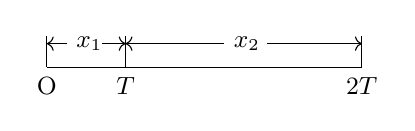
\begin{tikzpicture}
    \draw (0,0)--(4,0);
    \draw (0,0) node [anchor=north]{\small O}--(0,0.4);
    \draw (1,0) node [anchor=north]{\small $T$}--(1,0.4);
    \draw (4,0) node [anchor=north]{\small $2T$}--(4,0.4);
    \draw [<-](0,0.3)--(0.25,0.3) node [anchor=west]{\small $x_1$};
    \draw [->](0.7,0.3)--(1,0.3);
    \draw [<-](1,0.3)--(2.25,0.3) node [anchor=west]{\small $x_2$};
    \draw [->](2.8,0.3)--(4,0.3);
  \end{tikzpicture}
  \caption{等时间段内的位移差}
  \label{fig:Delta x}
\end{figure}

则有关系
\begin{equation}
x_2-x_1=aT^2
  \label{eq:Delta x}
\end{equation}
式\eqref{eq:Delta x} 不涉及初速度,一般用来处理用打点计时器所获得的纸带,因为纸带上的点是可以用毫米刻度尺来测量的,用这个方法求加速度很方便.

\subsubsection{证法一}
第一段中间时刻的瞬时速度等于第一段的平均速度,记为$v_1$,则$v_1=\cfrac{x_1}{T}$
第二段中间时刻的瞬时速度等于第二段的平均速度,记为$v_2$,则$v_2=\cfrac{x_2}{T}$
由\eqref{eq:acceleration}式得
$$a=\cfrac{v_2-v_1}{T}$$
将$v_1$和$v_2$的表达式代入得
$$a=\cfrac{x_2/T-x_1/T}{T}$$
上式分子分母同乘以$T$,然后左右同时再乘以$T^2$,移项得
$$x_2-x_1=aT^2$$
\subsubsection{证法二}
画出这段时间段内的$v-t$图象如下
\begin{figure}[H]
  \centering
  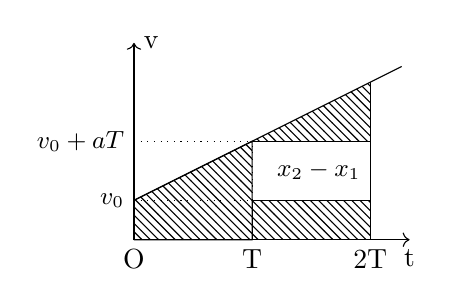
\begin{tikzpicture}
    \draw[->] (0,0) node [anchor=north]{O} -- (3.5,0) node [anchor=north]{t};
    \draw[->] (0,0)  -- (0,2.5) node [anchor=west]{v};
    \draw (0,0.5) -- (3.4,2.2);
    \draw [dotted] (1.5,0) node [anchor=north]{T}-- (1.5,1.25);
    \draw  (3,0) node [anchor=north]{2T} -- (3,2);
    \draw [dotted] (0,0.5)--(3,0.5);
    \draw [dotted] (1.5,1.25)--(3,1.25);
    \draw [pattern=north west lines] (0,0)--(1.5,0)--(1.5,1.25)--(0,0.5);
    \draw [pattern=north west lines] (1.5,1.25)--(3,1.25)--(3,2);
    \draw [pattern=north west lines] (1.5,0) rectangle (3,0.5);
    \draw (3,0.875) node [anchor=east] {\small $x_2-x_1$}; 
    \draw (0,0.5) node [anchor=east]{\small $v_0$};
    \draw [dotted] (0,1.25) node [anchor=east]{\small $v_0+aT$}--(1.5,1.25);
  \end{tikzpicture}
  \caption{相邻位移差}
  \label{fig:Delta xx}
\end{figure}

图\ref{fig:Delta xx} 中$0\sim T$ 时间段内梯形阴影面积表示位移$x_1$,$T\sim 2T$ 梯形面积表示位移$x_2$ 两面积之差就表示$x_2-x_1$,在图中所示为空白矩形的面积.矩形的长为$T$,宽为$aT$,所以其面积为$aT^2$,即
$$x_2-x_1=aT^2$$

\subsubsection{证法三}
设初速度为$v_0$,则由匀变速直线运动位移与时间的关系\eqref{eq:x-t}得
\begin{equation}
x_1=v_0T+\cfrac{1}{2}aT^2
  \label{eq:x1}
\end{equation}
\begin{equation}
x_1+x_2=v_0\cdot 2T+\cfrac{1}{2}a(2T)^2
  \label{eq:x2+x1}
\end{equation}
用式\eqref{eq:x2+x1}$-2\times$\eqref{eq:x1}得
$$x_2-x_1=aT^2$$

\subsubsection{证法四}
同证法三计算出第一段的位移,即式\eqref{eq:x1}.由匀变速直线运动速度与时间的关系\eqref{eq:v-t}得第二段的初速度为

$$v_1=v_0+aT$$

再由匀变速直线运动位移与时间关系\eqref{eq:x-t}计算第二段的位移得

\begin{equation}
x_2=(v_0+aT)\cdot T+\cfrac{1}{2}aT^2
  \label{eq:x2}
\end{equation}

用式\eqref{eq:x2} $-$ \eqref{eq:x1}得
$$x_2-x_1=aT^2$$

\subsection{逐差法求加速度}
我们首先说明为什么要用逐差法来处理问题,因为实验有误差,我们处理的原则是让误差尽可能小.一般毫米刻度尺的绝对误差是$1mm$,如图\ref{fig:rulemm}所示
\begin{figure}[H]
  \centering
  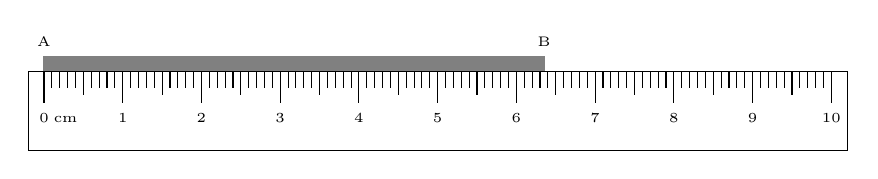
\begin{tikzpicture}
    \foreach \x in {
      0.1,0.2,0.3,0.4,0.6,0.7,0.8,0.9,
      1.1,1.2,1.3,1.4,1.6,1.7,1.8,1.9,
      2.1,2.2,2.3,2.4,2.6,2.7,2.8,2.9,
      3.1,3.2,3.3,3.4,3.6,3.7,3.8,3.9,
      4.1,4.2,4.3,4.4,4.6,4.7,4.8,4.9,
      5.1,5.2,5.3,5.4,5.6,5.7,5.8,5.9,
      6.1,6.2,6.3,6.4,6.6,6.7,6.8,6.9,
      7.1,7.2,7.3,7.4,7.6,7.7,7.8,7.9,
      8.1,8.2,8.3,8.4,8.6,8.7,8.8,8.9,
      9.1,9.2,9.3,9.4,9.6,9.7,9.8,9.9,
    }
    \draw (\x,0)--(\x,-0.2);
    \foreach \y in {0,1,2,3,4,5,6,7,8,9,10}
    \draw (\y,0)--(\y,-0.4) node [anchor=north]{\tiny \y};
    \foreach \z in {0.5,1.5,2.5,3.5,4.5,5.5,6.5,7.5,8.5,9.5}
    \draw (\z,0)--(\z,-0.3);
    \draw (-0.2,0) rectangle (10.2,-1);
    \draw (0,-0.6) node [anchor=west]{\tiny cm};
    \filldraw [color=gray] (0,0.02) rectangle (6.35,0.2);
    \draw (0,0.2) node [anchor=south]{\tiny A};
    \draw (6.35,0.2) node [anchor=south]{\tiny B};
  \end{tikzpicture}
  \caption{毫米刻度尺绝对误差}
  \label{fig:rulemm}
\end{figure}

在图\ref{fig:rulemm}中,测量一个杆的长度,使$A$ 端与零刻度线对齐,然后读$B$ 端的读数就是杆的长度.但是$B$不是完全与某一个刻度线对齐的,仔细观察不难发现它是一个介于$63mm$ 和$64mm$的数,所以坐标$x_B$ 的读数误差最大也就是$64mm-63mm=1mm$.对于一条纸带,我们在测量距离时,如图\ref{fig:zhidai}所示

\begin{figure}[H]
  \centering
  \begin{tikzpicture}
    \foreach \x in {
      0.1,0.2,0.3,0.4,0.6,0.7,0.8,0.9,
      1.1,1.2,1.3,1.4,1.6,1.7,1.8,1.9,
      2.1,2.2,2.3,2.4,2.6,2.7,2.8,2.9,
      3.1,3.2,3.3,3.4,3.6,3.7,3.8,3.9,
      4.1,4.2,4.3,4.4,4.6,4.7,4.8,4.9,
      5.1,5.2,5.3,5.4,5.6,5.7,5.8,5.9,
      6.1,6.2,6.3,6.4,6.6,6.7,6.8,6.9,
      7.1,7.2,7.3,7.4,7.6,7.7,7.8,7.9,
      8.1,8.2,8.3,8.4,8.6,8.7,8.8,8.9,
      9.1,9.2,9.3,9.4,9.6,9.7,9.8,9.9,
    }
    \draw (\x,0)--(\x,-0.2);
    \foreach \y in {0,1,2,3,4,5,6,7,8,9,10}
    \draw (\y,0)--(\y,-0.4) node [anchor=north]{\tiny \y};
    \foreach \z in {0.5,1.5,2.5,3.5,4.5,5.5,6.5,7.5,8.5,9.5}
    \draw (\z,0)--(\z,-0.3);
    \draw (-0.2,0) rectangle (10.2,-1);
    \draw (0,-0.6) node [anchor=west]{\tiny cm};
    \draw (-0.2,-0.4)--(-0.4,-0.4)--(-0.4,0.5)--(10.4,0.5)--(10.4,-0.4)--(10.2,-0.4);
    \foreach \x in {0,0.2,0.8,1.8,3.2,5,7.2,9.8}
    \filldraw [color=black] (\x , 0.05) circle [radius=1pt];
    \foreach \x in {0,0.2,0.8,1.8,3.2,5,7.2,9.8}
    \draw (\x , 0.05) node [anchor=south] {\tiny \thepointnum\stepcounter{pointnum}};
  \end{tikzpicture}
  \caption{测量纸带上点的距离}
  \label{fig:zhidai}
\end{figure}

在图\ref{fig:zhidai}中,使纸带上的计数点$0$ 与刻度尺上的零刻度对齐,然后依次读取其它点的读数,这些读数记作$x_i' \quad (i=0,1,2 \cdots)$,在纸带上标出这些读数如\ref{fig:zhidaidushu}所示

\setcounter{pointnum}{0}
\begin{figure}[H]
  \centering
  \begin{tikzpicture}
    \draw (-0.4,-0.4) rectangle (10.4,0.5); 
    \foreach \x in {0,0.2,0.8,1.8,3.2,5,7.2,9.8}
    \filldraw [color=black] (\x , 0.05) circle [radius=1pt];
    \foreach \x in {0,0.2,0.8,1.8,3.2,5,7.2,9.8}
    \draw (\x , 0.05) node [anchor=south] {\tiny \thepointnum\stepcounter{pointnum}};
    \draw (0,0)--(0,-0.8);
    \draw (0.2,0)--(0.2,-0.15);
    \draw [->,>=stealth] (0,-0.1)--(0.2,-0.1) ;
    \draw (0.2,-0.15) node {\tiny $x_1'$};
    \draw (0.8,0)--(0.8,-0.25);
    \draw [->,>=stealth] (0,-0.2)--(0.8,-0.2); 
    \draw (0.8,-0.3) node [anchor=south east] {\tiny $x_2'$};
    \draw (1.8,0)--(1.8,-0.35);
    \draw [->,>=stealth] (0,-0.3)--(1.8,-0.3) node [anchor=south east] {\tiny $x_3'$};
    \draw (3.2,0)--(3.2,-0.45);
    \draw [->,>=stealth] (0,-0.4)--(3.2,-0.4)node [anchor=south east] {\tiny $x_4'$};
    \draw (5,0)--(5,-0.55);
    \draw [->,>=stealth] (0,-0.5)--(5,-0.5)node [anchor=south east] {\tiny $x_5'$};
    \draw (7.2,0)--(7.2,-0.65);
    \draw [->,>=stealth] (0,-0.6)--(7.2,-0.6)node [anchor=south east] {\tiny $x_6'$};
    \draw (9.8,0)--(9.8,-0.75);
    \draw [->,>=stealth] (0,-0.7)--(9.8,-0.7)node [anchor=south east] {\tiny $x_7'$};
  \end{tikzpicture}
  \caption{计数点的读数标记}
  \label{fig:zhidaidushu}
\end{figure}

我们以不带撇号的坐标表示两点间的距离,如图\ref{fig:zhidaijvli}所示

\setcounter{pointnum}{0}
\begin{figure}[H]
  \centering
  \begin{tikzpicture}
    \draw (-0.4,-0.4) rectangle (10.4,0.5); 
    \foreach \x in {0,0.2,0.8,1.8,3.2,5,7.2,9.8}
    \filldraw [color=black] (\x , 0.05) circle [radius=1pt];
    \foreach \x in {0,0.2,0.8,1.8,3.2,5,7.2,9.8}
    \draw (\x , 0.05) node [anchor=south] {\tiny \thepointnum\stepcounter{pointnum}};
    \draw [<-,>=stealth] (0.2,0.05)--(0.4,0.05);
    \draw (0.5,0.05) node {\tiny $x_2$};
    \draw [->,>=stealth] (0.6,0.05)--(0.8,0.05);
    \draw [<-,>=stealth] (0.8,0.05)--(1.15,0.05);
    \draw (1.3,0.05) node {\tiny $x_3$};
    \draw [->,>=stealth] (1.45,0.05)--(1.8,0.05);
    \draw [<-,>=stealth] (1.8,0.05)--(2.35,0.05);
    \draw (2.5,0.05) node {\tiny $x_4$};
    \draw [->,>=stealth] (2.65,0.05)--(3.2,0.05);
    \draw [<-,>=stealth] (3.2,0.05)--(3.95,0.05);
    \draw (4.1,0.05) node {\tiny $x_5$};
    \draw [->,>=stealth] (4.25,0.05)--(5,0.05);
    \draw [<-,>=stealth] (5,0.05)--(5.95,0.05);
    \draw (6.1,0.05) node {\tiny $x_6$};
    \draw [->,>=stealth] (6.25,0.05)--(7.2,0.05);
    \draw [<-,>=stealth] (7.2,0.05)--(8.35,0.05);
    \draw (8.5,0.05) node {\tiny $x_7$};
    \draw [->,>=stealth] (8.65,0.05)--(9.8,0.05);
  \end{tikzpicture}
  \caption{计数点的距离标记}
  \label{fig:zhidaijvli}
\end{figure}

由于我在这里作图是按照标准的$1:3:5:7:9:11$ 完成的,第一段的距离太小,为了防止第一段看不清楚,所以在第一段上没有标出$x_1$,同时由图 \ref{fig:zhidaidushu}和图\ref{fig:zhidaijvli}对比可知两种表示方法的关系为

\begin{equation}
  x_i=x_i'-x_{i-1}' \qquad (i=1,2,3 \cdots)
  \label{eq:dushujvli}
\end{equation}

下面我们讨论加速度的计算,由$x_2$ 和$x_1$ 我们可以计算加速度,如下
\begin{gather}
  x_2-x_1=a_1T^2
  \intertext{经过简单计算可得}
  a_1=\frac{x_2-x_1}{T^2}
  \intertext{同理也可以得到加速度}
  a_2=\frac{x_3-x_2}{T^2}\\
  a_3=\frac{x_4-x_3}{T^2}\\
  a_4=\frac{x_5-x_4}{T^2}
  \intertext{由于在$a_1$的分子部分需要三个坐标来确定这个差,所以它的误差为$3mm$,$a_2$和$a_3$需要四个坐标来确定分子部分的差,所以其误差为$4mm$,但$T$是相同的,下面我们将这四个加速度取几何平均,则得到}
  a_{1234}=\frac{1}{4}(a_1+a_2+a_3+a_4)=\frac{x_5-x_1}{4T^2}
  \intertext{上面这个平均加速度,其分子部分需要三个坐标确定,但是分子上需要除以$4$,所以它的误差为$3mm/4=0.75mm$,同理我们可以得到$a_{2345}$等类似的平均值,如下}
  a_{2345}=\frac{1}{4}(a_2+a_3+a_4+a_5)=\frac{x_6-x_2}{4T^2}\\
  a_{3456}=\frac{1}{4}(a_3+a_4+a_5+a_6)=\frac{x_7-x_3}{4T^2}
  \intertext{上面的$a_{2345}$和$a_{3456}$的分子部分需要4个坐标确定,所以它们的误差是$4mm/4=1mm$,但是如果再取一次平均,如下}
  a=\frac{1}{3}(a_{1234}+a_{2345}+a_{3456})=\frac{(x_5+x_6+x_7)-(x_1+x_2+x_3)}{3\times 4T^2}
  \intertext{上式分子部分等于$x_7'-x_4'-x_3'$,用到了三个读数,但是分母上需要除以$12$ 所以它的误差是$3mm/12=0.25mm$,所以最后这个结果误差是最小的,为我们所采纳,这就是逐差法公式.下面我们总结写出加速度的方法,分母上的这个数值可以这样来确定:分子中的括号中有$3$个数值,同时每个数值的下标差相同(比如$5-1=4$,$6-2=4$,$7-3=4$),分母上的这个数值就是$3\times4=12$,同理我们可以写出$6$段和$9$段的计算公式如下}
  a=\frac{(x_4+x_5+x_6)-(x_1+x_2+x_3)}{3\times3 T^2}\\
  a=\frac{(x_6+x_7+x_8+x_9)-(x_1+x_2+x_3+x_4)}{4\times5 T^2}
  \intertext{有许多人为了方便记住逐差法的公式,在偶数段时将纸带一分为二,比如$6$段时,可以写作}
  a=\frac{(x_4+x_5+x_6)-(x_1+x_2+x_3)}{(3T)^2}
  \intertext{这可以理解为时间间隔为$3T$ 的两大段,使用$\Delta x=aT^2$ 一步写出,但是在遇到奇数段(比如$7$段)的时候就会遇到麻烦,如果按这个逻辑,可以选用前$6$段或者后$6$段,这样写出的公式误差是$3mm/9=0.33mm$,而按逐差法写出的公式是\CJKunderwave{去掉中间一段}这样计算的结果误差为$3mm/12=0.25mm$,显然\CJKunderwave{去掉中间一段}才能得到更精确的答案.}
  \notag
\end{gather}

\subsection{初速度为零的比例关系}

匀变速直线运动的比例关系共有两大组,其一按\CJKunderwave{时间等分},其二按\CJKunderwave{位移等分}.

\subsubsection{按时间等分}

时间每隔 $T$ 分一份,则 $T$ ,$2T$,$3T$,$\cdots$ 等时刻对应的速度分别为 $v_1$,$v_2$,$v_3$,$\cdots$

由\eqref{eq:v-t} 式,可得
\[
  v_n=a\cdot nT
\]

所以有

\begin{equation}
  v_1 : v_2 :v_3 : \cdots : v_n = 1 : 2 : 3 :\cdots  : n 
  \label{eq:v-frac}
\end{equation}

从0时刻开始,$0\sim T$, $0\sim 2T$, $0\sim 3T $ ,$ \cdots$ 等时间间隔内对应的位移分别记为 $x_1$ , $x_2$ , $x_3$, $\cdots$

由 \eqref{eq:x-t} 式,可得

\[
  x_n=\cfrac{1}{2}a\cdot (nT)^2
\]

所以有

\begin{equation}
  x_1 : x_2 :x_3 : \cdots : x_n = 1^2 : 2^2 : 3^2 :\cdots  : n^2 
  \label{eq:x-frac}
\end{equation}

第 $T$ ,第 $2T$ ,第 $3T$ , $\cdots$ ,第 $nT$ 时间间隔内对应的位移分别记为
$\Delta x_1$ , $\Delta x_2$ , $\Delta x_3$, $\cdots$ , $\Delta x_n$

由$x_n$ 与 $n$ 的关系可得
\[
  \Delta x_n =x_n-x_{n-1}=(2n-1)\cdot \cfrac{1}{2}aT^2
\]

所以有

\begin{equation}
 \Delta x_1 :\Delta x_2 :\Delta x_3 : \cdots :\Delta x_n 
 = 1 : 3 : 5 :\cdots  : (2n-1)
  \label{eq:Delta x-frac}
\end{equation}

\subsubsection{按位移等分}

位移每隔$L$ 分一份,记 $L$ ,$2L$ , $3L$ , $\cdots $ , $nL$ 等位置时,质点的速度分别为 $v_1$ , $v_2$ ,$v_3$ , $\cdots$ , $v_n$ 

由\eqref{eq:x-v} 式,可得

\[v_n^2-0=2ax_n\]

代入 $x_n=nL$ 解得
\[
  v_n=\sqrt{n\cdot 2aL}
\]

所以有

\begin{equation}
  v_1 : v_2 : v_3 : \cdots : v_n =\sqrt{1} : \sqrt{2} :\sqrt{3} :\cdots :\sqrt{n} 
  \label{eq:v-x-frac}
\end{equation}

记质点到达 $L$ ,$2L$ , $3L$ , $\cdots $ , $nL$ 等位置时,需要的时间分别为 $t_1$ , $t_2$ ,$t_3$ , $\cdots$ , $t_n$ 

由\eqref{eq:x-t} 式,可得
\[x_n=\cfrac{1}{2}at_n^2\]

代入 $x_n=nL$ 解得
\[
  t_n=\sqrt{\cfrac{2nL}{a}}
\]

所以有

\begin{equation}
  t_1 : t_2 : t_3 : \cdots : t_n =\sqrt{1} : \sqrt{2} :\sqrt{3} :\cdots :\sqrt{n} 
  \label{eq:t-x-frac}
\end{equation}

记质点经过第一个 $L$ ,第二个$L$, 第三个$ L$ , $\cdots$ ,第$n$ 个 $L$ 等位移时,需要的时间分别为$\Delta t_1$ , $\Delta t_2$ ,$\Delta t_3$ , $\cdots$ , $\Delta t_n$ 

由$t_n$ 的表达式可得
\[
  \Delta t_n = t_n - t_{n-1}=(\sqrt{n}-\sqrt{n-1})\sqrt{\cfrac{2L}{a}}
\]

所以有

\begin{equation}
  \Delta t_1 : \Delta t_2 : \Delta t_3 : \cdots : \Delta t_n =\sqrt{1} : (\sqrt{2}-\sqrt{1}) :(\sqrt{3}-\sqrt{2}) :\cdots :(\sqrt{n}-\sqrt{n-1} )
  \label{eq:Delta t-x-frac}
\end{equation}

  \newpage
  \section{匀变速直线运动习题精解}
\begin{calculate}
  1.一物体以某一速度冲上一光滑斜面,做匀变速直线运动,前$4s$ 的位移为$1.6m$ ,随后$4s$ 的位移为零,那么物体的加速度多大?

  a.物体的加速度大小为$0.1m/s^2$

  e.题目中所述运动情况如<:
  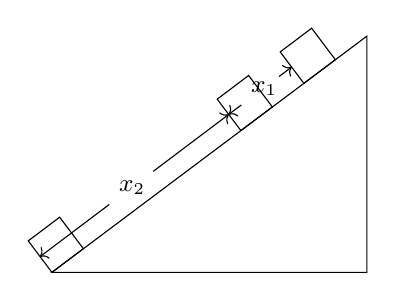
\begin{tikzpicture}
   \draw (0,0)--(4,0)--(4,3)-- cycle; 
   \draw[rotate=37] (0,0) rectangle (0.5,0.5);
   \draw[xshift=2.4cm ,yshift=1.8cm ,rotate=37] (0,0) rectangle (0.5,0.5);
   \draw[xshift=3.2cm ,yshift=2.4cm ,rotate=37] (0,0) rectangle (0.5,0.5);
   \draw[<-,rotate=37](0,0.25)--(1.1,0.25) node [anchor= south west] {\small $x_2$};
   \draw[->,rotate=37](1.8,0.25)--(3,0.25);
   \draw [<-,rotate=37] (3,0.25)--(3.2,0.25) node [anchor=south west]{\small $x_1$};
   \draw [->,rotate=37] (3.8,0.25)--(4,0.25);
  \end{tikzpicture}
  :>所示.由于随后的$4s$ 内位移为零,则可以判断出在这$4s$ 内先上升再下降,由对称性知向上运动$x_1$ 和向下运动 $x_1$的时间都是$2s$.所以记发生$x_2$ 位移的时间$t_2=4s$,发生$x_1$位移的时间 $t_1=2s$.
  \newline
  解法一:设初速度$v_0$,由匀变速直线运动位移与时间的关系\eqref{eq:x-t}式得
  $$x_2=v_0t_2+\cfrac{1}{2}at_2^2$$
  显然可以得到,物体到达最高点的速度为$0$ , 设从最低点到最高点所用时间为$t$ ,则$t=t_1+t_2=6s$,同样可以由\eqref{eq:x-t}式得
  $$x_1+x_2=v_0t+\cfrac{1}{2}at^2$$
  由上述二式联立解得
  \newline
  $$a=-0.1m/s^2 , v_0=0.6m/s$$

  ee.解法二:由平均速度公式\eqref{eq:v-average-half}可以得到前$4s$ 内的中间时刻的瞬时速度为 
  $$v=\cfrac{x_2}{t_2}=0.4m/s$$
  根据后 $2s$ 速度减到零,可得从第$2s$末到第$6s$末速度由$v=0.4m/s$ 减到零.所以可以由加速度定义\eqref{eq:acceleration}式得
  $$a=\cfrac{\Delta v}{\Delta t}=\cfrac{0-0.4m/s}{6s-2s}=-0.1m/s^2$$

  ee.解法三:将此运动视为反向的初速度为零的匀加速直线运动,由等分时间时位移的比例关系\eqref{eq:x-frac}可得,连续三段$T=2s$的位移比为$1:3:5$ ,所以可以得到
  $$x_1=\cfrac{1}{8}x_2=0.2m$$
 同时可以得到第二段时间内的位移为$0.6m$, 由相邻两段时间内的位移差公式\eqref{eq:Delta x} 得
  $$0.6m-0.2m=a^\prime (2s)^2$$
  解上式得
  $$a^\prime =\cfrac{0.6m-0.2m}{4s^2}=0.1m/s^2$$
  上式中加速度加撇的原因在于它是反向的匀加速直线运动,而正向的匀减速直线运动与它相差一个负号,即$a=-a'=-0.1m/s^2$.

  ee.解法四:考虑同第三种解法得到$x_1=0.2m$ ,仍然视为反向的匀加速直线运动,由匀变速直线运动公式\eqref{eq:x-t}关系得
  $$x_1=\cfrac{1}{2}a'T^2$$
  对上式简单运算得
  $$a'=\cfrac{2x_1}{T^2}=0.1m/s^2$$
  匀减速直线运动的加速度为$a=-a'=-0.1m/s^2$.

  ee.解法五:与解法二相同,由平均速度公式\eqref{eq:v-average-half}式得到中间时刻的瞬时速度$v=0.4m/s$,对于此后$4s$ 内物体将匀减速到速度为$0$,由平均速度公式\eqref{eq:average}可得后$4s$ 的位移为
  $$x=\cfrac{v+0}{2}\cdot t =0.8m$$
  由匀变速直线运动位移与速度的关系\eqref{eq:x-v}式得
  $$v^2-0^2=2ax$$
  解得
  $$a=-\cfrac{v^2}{2x}=-0.1m/s^2$$

  ee.同学们注意,在匀变速直线运动中往往会导致一题多解,但是归根结底都是相同的.只是按不同的思路考虑问题罢了,如果方法选择得当则题目会很轻松的得到解决,但是选择不当会增加不少的计算量.所以同学们在刚刚开始学习的时候最好能够尝试一题多解,练熟公式的同时找到解题的技巧.

  

\end{calculate}
\begin{calculate}
  2.一物体做匀加速直线运动,通过一段位移$\Delta x$ 所用的时间为$t_1$ ,紧接着通过下一段位移$\Delta x$ 所用时间为$t_2$ ,求物体运动的加速度.

  a.$\cfrac{2\Delta x(t_1-t_2)}{t_1t_2(t_1+t_2)}$

  e.物体通过第一段位移中间时刻的瞬时速度为$v_1=\frac{\Delta x}{t_1}$ ,通过第二段位移中间时刻的瞬时速度为$v_2=\frac{\Delta x}{t_2}$ ,由$v_1$ 变到$v_2$ 所需的时间显然为 $\Delta t=\frac{t_1+t_2}{2}$ ,由加速度定义\eqref{eq:acceleration} 式得
  $$a=\cfrac{v_2-v_1}{\Delta t}=\cfrac{2\Delta x(t_1-t_2)}{t_1t_2(t_1+t_2)}$$

  3.一质点运动的位移随时间变化的图象是一条抛线,方程为$x=-5t^2+40t$,则
  [1]求质点的初速度
  [2]求质点运动的加速度
  [3]求质点运动的最大位移
  [4]求质点速度为零时的时间

  a.见解析

  e.对比$x=-5t^2+40t$ 和 匀变速直线运动位移与时间的关系\eqref{eq:x-t} 可得

  ee.(1)质点运动的初速度为$v_0=40m/s$

  ee.(2)质点运动的加速度由对比可知$\frac{1}{2}a=-5m/s^2$,解得$a=-10m/s^2$.

  ee.(3)最大位移由匀变速直线运动\eqref{eq:x-v}式得
  $$0-v_0^2=2ax_m$$
  解得
  $$x_m=\cfrac{0-v_0^2}{2a}=80m$$
  
  ee.(4)由匀变速直线运动速度与时间的关系\eqref{eq:v-t}式得
  $$0=v_0+at$$
  解得
  $$t=-\cfrac{v_0}{a}=4s$$

  4.一辆汽车沿平直公路以速度$v_1$ 行驶了$\frac{2}{3}$ 的路程,接着又以速度$v_2=20km/h$ 行驶完其余 $\frac{1}{3}$ 的路程,如果汽车全程的平均速度为$28km/h$ ,那么汽车在前 $\frac{2}{3}$ 的路程内速度的大小为多少?

  a.$35km/h$

  e.由于汽车做单向直线运动则位移大小等于路程,设总位移为$x$ , 则前$\frac{2}{3}$ 所用的时间为 $t_1=\frac{2x}{3v_1}$ , 后 $\frac{1}{3}$ 所用时间为 $t_2=\frac{x}{3v_2} $ ,则总时间为 
  $$t=t_1+t_2=\cfrac{2x}{3v_1}+\cfrac{x}{3v_2}$$
  由平均速度公式 \eqref{eq:average} 得
  $$\overline{v}=\cfrac{x}{\frac{2x}{3v_1}+\frac{x}{3v_2}}$$
  上式约掉$x$ 然后经过简单计算得
  $$v_1=\cfrac{2\overline{v}v_2}{3v_2-\overline{v}}=35km/h$$
  注意:在这个题的计算中不要上来就化单位为国际单位,因为在计算中很明显的一点就是位移不知道,所以在计算中一定可以消去.这样一来,最后的结果应该就可以用与题目中相同的单位表达,并且一般会比较简洁,如果化单位的话,这个题目就走了弯路了.

  5.质点由A点静止出发沿直线 AB运动,行程的第一部分是加速度大小为 $a_1$ 的匀加速运动,接着做加速度大小为$a_2$ 的匀减速运动,到达B点时恰好速度减为零.若AB间总长度为$x$ , 则质点从A到B所用时间$t$ 为多少?

  a.$\sqrt{\cfrac{2x(a_1+a_2)}{a_1a_2}}$

  e.设第一阶段的末速度为$v$ , 则由题意据匀变速直线运动位移与速度关系\eqref{eq:x-v} 式可知:
  $$\cfrac{v^2}{2a_1}+\cfrac{v^2}{2a_2}=x$$
  由上式解得
  $$v=\sqrt{\cfrac{2a_1a_2x}{a_1+a_2}}$$
  而由匀变速直线运动位移计算基本关系\eqref{eq:displacement}式可得
  $$x=\cfrac{0+v}{2}t_1+\cfrac{v+0}{2}t_2=\cfrac{v}{2}t$$
  由此解得
  $$t=\sqrt{\cfrac{2(a_1+a_2)x}{a_1a_2}}$$

  6.美国``肯尼迪''号航空母舰上装有帮助飞机起飞的弹射系统.已知``F-15'' 型战斗机在跑道上加速时,产生的最大加速度为$5m/s^2$ ,起飞的最小速度是$50m/s^2$ ,弹射系统能够使飞机具有的最大速度为$30m/s$ ,则:
  [1]飞机起飞时在跑道上至少加速多长时间才能起飞?
  [2]航空母舰的跑道至少应该多长?

  a. (1)$4s$ (2)$160m$

  e.(1)飞机在跑道上运动的过程中,当有最大初速度、最大加速度时,起飞所需时间最短,据加速度的定义\eqref{eq:acceleration}或者匀变速直线运动速度与时间的关系\eqref{eq:v-t}得
  $$t=\cfrac{v-v_0}{a}=\cfrac{50-30}{5}s=4s$$
  则飞机起飞时在跑道上的加速时间至少为$4s$.

  ee.(2)由匀变速直线运动位移与时间的关系\eqref{eq:x-v} 式得
  $$x=\cfrac{v^2-v_0^2}{2a}=\cfrac{50^2-30^2}{2\times 5}m=160m$$
  即航空母舰的跑道至少为$160$.

  7.一质点做匀变速直线运动,初速度$v_0=2m/s$ , $4s$ 内位移为$20m$ ,求:
  [1]质点$4s$末的速度;
  [2]质点$2s$ 末的速度.

  a.(1)$8m/s$ (2) $5m/s$

  e.(1)利用平均速度公式\eqref{eq:average velocity}得$4s$ 内的平均速度为
  $$\overline{v}=\cfrac{x}{t}=\cfrac{v_0+v_4}{2}$$
  代入数据解得$4s$末的速度为
  $$v_4=8m/s$$

  ee.(2)由匀变速直线运动平均速度与位移中点的瞬时速度关系\eqref{eq:v-average-half}得$2s$ 末的速度为
  $$v_2=\cfrac{v_0+v_4}{2}=5m/s$$

  8.一个做匀加速直线运动的物体,在前$4s$ 内经过的位移为$24m$ ,在第$2$ 个$4s$ 内经过的位移是$60m$ ,求这个物体的加速度和初速度各是多少?

a.$2.25m/s^2$ $1.5m/s$

e.解法一:物体在前$4s$ 内的位移 
$$x_1=v_0t+\frac{1}{2}at^2$$
在第2个$4s$ 内的位移
$$x_2=v_0(2t)+\cfrac{1}{2}(2t)^2-(v_0t+\cfrac{1}{2}at^2)$$
将$x_1=24m$ ,$x_2=60m$ 代入上式,解得
$$a=2.25m/s^2,v_0=1.5m/s$$

ee.解法二:物体在$8s$ 内的平均速度等于中间时刻(第$4s$ 末)的瞬时速度,则
$$v_4=\cfrac{24+60}{8}m/s=10.5m/s$$
物体在前$4s$ 内的平均速度等于第$2s$ 末的瞬时速度
$$v_2=\cfrac{24}{4}m/s=6m/s$$
由加速度的定义可得
$$a=\cfrac{v_4-v_2}{\Delta t}=\cfrac{10.5-6}{2}m/s^2=2.25m/s^2$$
由匀变速直线运动速度与时间的关系得
$$v_2=v_0+at_2$$
解得
$$v_0=v_2-at_2=1.5m/s$$

ee.解法三:由等时相邻位移公式\eqref{eq:Delta x}得
$$a=\cfrac{\Delta x}{T^2}=\cfrac{60-24}{4^2}m/s^2=2.25m/s^2$$
同解法一$v_4=\frac{24+60}{8}m/s$,由匀变速直线运动速度与时间关系\eqref{eq:v-t} 式得
$$v_4=v_0+at_4$$
解得
$$v_0=1.5m/s$$

9.一辆汽车以$3m/s^2$ 的加速度开始启动的瞬间,另一辆以$6m/s$ 的速度做匀速直线运动的自行车恰好从汽车的旁边通过.
[1]汽车一定能追上自行车吗?若能追上,汽车经过多长时间追上?追上时汽车的瞬时速度多大?
[2]记汽车用2表示,自行车用1表示.在汽车追上自行车前,当$v_2<v_1$ 时,两者间的距离如何变化?当$v_2>v_1$时,两者间的距离如何变化?汽车追上自行车前多长时间与自行车相距最远?此时的距离是多大?

a.见解析

e.解法一:(1)因为汽车做加速运动,故汽车一定能追上自行车.汽车追上自行车时,两者位移相等,$x_2=x_1$,即
$$\cfrac{1}{2}at^2=v_1t$$
解得
$$t=\cfrac{2v_1}{a}=\cfrac{2\times6}{3}s=4s,v_2=at=3\times 4 m/s=12m/s$$

ee.(2)开始阶段,$v_2<v_1$ ,两者间的距离逐渐变大.后来$v_2>v_1$ ,两都间的距离又逐渐减小.所以汽车追上自行车前,当$v_2=v_1$ 时,两者距离最大.设经过时间$t_1$ ,汽车速度等于自行车速度,则
$$at_1=v_1$$
解得
$$t_1=2s$$
此时
$$x_1=v_1t_1=6\times2m=12m$$
$$x_2=\cfrac{1}{2}at_1^2=\cfrac{1}{2}\times3\times2^2m=6m$$
最大距离为
$$\Delta x=x_1-x_2=6m$$

ee.解法二:在第一个解法中偏重于物理情景的讨论,由于运动的情况可能要复杂的多,讨论就会变得复杂,所以这里介绍偏重数学计算的统一化讨论的方法.开始自行车在汽车前面,则分别写出二者在任意时刻$t$ 的位移分别为
$$x_1=v_1t , x_2=\cfrac{1}{2}at^2$$
由于自行车开始在汽车的前面,所以计算它们位移差的变化量 $\Delta x=x_1-x_2$ ,如果$\Delta x <0 $ 在$t>0$ 时成立,则汽车就可以追上自行车,反之则不能追上.
$$\Delta x=v_1t-\cfrac{1}{2}at^2$$
代入数值得$\Delta x $关于时间$t$ 的一元二次函数.如下
$$\Delta x=6t-\cfrac{3}{2}t^2, (t>0)$$
令$$\Delta x =0 $$ 得一元二次方程
$$6t-\cfrac{3}{2}t^2=0$$
上式容易解得$t_1=0 (\mbox{舍去}),t_2=4s$ ,所以经过$4s$ 汽车追上自行车.此时速度为
$$v=at_2=3\times 4 m/s=12m/s$$

ee.求函数$\Delta x=6t-\cfrac{3}{2}t^2, (t>0)$的极大值,则由二次函数的性质易得
$$t=-\cfrac{6}{2\times(-\frac{3}{2})}s=2s$$
时二车的相对距离$\Delta x$ 取最大,为
$$\Delta x_{max}=\cfrac{4\times(-\frac{3}{2})\times 0 - 6^2}{4\times(-\frac{3}{2})}=6m$$


10.车从静止开始以$1m/s^2$ 的加速度前进,在车开始运动的同时,车后$20m$ 处,某人骑自行车开始以$ 6m/s$ 的速度匀速追赶,能否追上?若不能追上,人与车的最小距离是多少?若能追上,什么时候追上?

a.不能 $2m$

e.开始运动时,车在前,人在后所以选择人的起点为坐标原点,以车和人运动的方向为正方向,则以2表示车,1表示人,则二者的位移分别为
$$x_1=6t$$
$$x_2=20+\cfrac{1}{2}\times 1\times t^2$$
任意时刻二者位移差为 $\Delta x = x_2-x_1$ 代入上述表达式得
$$\Delta x= 0.5t^2-6t +20 ,(t>0)$$
令$\Delta x=0$ 得一元二次方程,其判别式为
$$\Delta = (-6)^2-4\times 0.5 \times 20 =-4<0$$
所以无解,则人不能追上汽车.
由一元二次函数求极值可得
$$\Delta x_{min}=\cfrac{4\times 0.5 \times 20 - (-6)^2}{4\times 0.5}=2m$$

11.一滴雨滴从离地面 $20m$ 高的楼房屋檐自由下落,下落过程中用 $0.2s$ 的时间通过一个窗口,窗口的高度为 $2m$ , $g$ 取 $10m/s^2$ ,问:
[1]雨滴落地时的速度大小;
[2]雨滴落地前最后 $1s$ 内的位移大小;
[3]屋檐离地面的上边框有多高?

a.见解析

e.(1)由匀变速直线运动速度与位移的关系可得
$$v^2=2gh \Longrightarrow v=\sqrt{2gh}=20m/s$$

ee.(2)法一:雨滴在最后$1s$内的平均速度等于中间时刻的瞬时速度,中间时刻到最后共经历 $t_1=0.5s$ 所以有
$$v=\overline{v}+gt_1 \Longrightarrow \overline{v}=v-gt_1=15m/s$$
由位移等于平均速度乘以时间得
$$\Delta h=\overline{v}\Delta t_1 =15m$$

ee.法二:仍然采用平均速度的方法,先求出总时间,然后再求出最后$1s$的中间时刻,即
$$h=\frac{1}{2}gt^2 \Longrightarrow t=\sqrt{\frac{2h}{g}}=2s$$
所以最后$1s$ 的中间时刻即 $t=1.5s$ 时瞬时速度等于平均速度
$$\overline{v}=gt=15m/s$$
由位移等于平均速度乘以时间得
$$\Delta h=\overline{v}\Delta t_1 =15m$$

ee.法三:先求出总时间,然后再算出前 $1s$ 的时刻,并求出位移和总位移作差也可以得到最后 $1s$ 内的位移.即
$$h=\frac{1}{2}gt^2 \Longrightarrow t=\sqrt{\frac{2h}{g}}=2s$$
从下落开始到落地前$1s$经历的时间为$t_1=1s$ ,所以
$$h_1=\frac{1}{2}gt_1^2=5m$$
最后$1s$ 内的位移为
$$\Delta h=h-h_1=20m-5m=15m$$


ee.(3)在雨滴通过窗口的过程中,用时$0.2s$,所以它的中间时刻的瞬时速度等于平均速度为
$$\overline{v'}=\frac{2m}{0.2s}=10m/s$$
所以雨滴由屋檐到通过窗口的中间时刻所用时间为
$$t_0=\frac{\overline{v'}}{g}=1s$$
由此可得,雨滴由屋檐到窗口的时间为$t'=1s-0.1s=0.9s$ 所以屋檐离窗口上边框的高度为
$$h'=\frac{1}{2}gt'^2=4.05m$$

12.一辆值勤的警车停在公路边,当警员发现从他旁边以$10m/s$ 的速度匀速行驶的货车严重超载时,决定前去追赶,经过$5.5s$ 后警车发动起来,并以$2.5m/s^2$的加速度做匀加速运动,但警车的行驶速度必须控制在$90km/h$以内,问:
[1]警车在追赶货车的过程中,两车的最大距离是多少?
[2]警车发动后要经过多长时间 才能追上货车?

a.(1) 75m \qquad (2) 12s

e.(1)以警车发动起来作为计时起点,首先将警车的最大速度切换成国际单位 $90km/h=25m/s$ ,则警车的加速过程的持续时间$t_m$ 为
$$v_m=at_m \Longrightarrow t_m=\frac{v_m}{a}=10s$$
写出$0\sim 10s$ 内两车的距离为
$$\Delta x=55+10t -\frac{5}{4}t^2$$
整理成标准一元二次方程
$$\Delta x =-\frac{5}{4}t^2+10t+55 \quad (m)$$
由二次函数的知识,易得在$0\sim 10s$内 $t=4s$ 时距离最大,为
$$\Delta x_{max}=75m$$

ee.注意,在警车追赶货车的过程中,要分两步考虑,在$0\sim 10s$ 内,两车的距离关系才是上述的一元二次函数,但是这个过程不一定就追上,所以不能直接使用$\Delta x=0$ 来计算出时间,这就导致错误了!! 最好的方法就是画出这段时间内的函数图象,然后得出能否在 $10s$ 内追上的明确结论.容易得到 $t=10s$ 时
$$\Delta x'=-\frac{5}{4}\times 10^2 +100 +55m =30m$$
于是加速过程结束时,警车没有追上货车,所以还要匀速追一段时间$t'$ 所以
$$t'=\cfrac{\Delta x'}{v_2-v_1}=2s$$
则警车追赶货车共用时间为
$$t=t_m+t'=12s$$

13.某人骑自行车以$v_1=4m/s$ 的速度前进,某时刻在他前面$x_0=7m$ 处有以$v_1=10m/s$ 的速度同向行驶的汽车开始关闭发动机减速前进,而以$a=-2m/s^2$ 的加速度匀减速前进,求:
[1]此人追上汽车之前落后于汽车的最大距离?
[2]此人需要多长时间才能追上汽车?

a.(1) 16m \qquad (2) 8s

e.(1)此问题出现了刹车,所以先求出刹车时间$t_s$
$$0=v_0+at_s \Longrightarrow t_s=-\frac{v_0}{a}=5s$$
容易写出$0\sim 5s$ 内两车的距离为
$$\Delta x = (7+10t-t^2)-4t $$
化成标准形式
$$\Delta x=-t^2+6t+7 \quad (m)$$
由一元二次方程得$t=3s$ 时,二者距离最大为
$$\Delta x_{max}=16m$$

ee.(2)注意,只有在$0\sim 5s$ 内二者的距离才按上述方程变化,但是不能保证$5s$ 内一定能追上,这需要单独判断.易得$t=5s$ 时,二者距离为
$$\Delta x'=-5^2+6\times 5 +7 m =12m$$
在$5s$时,人还没有追上汽车,而这时汽车已经停止运动,所以剩下的这$12m$ 人需要匀速追击,其所需时间$t'$ 为
$$t'=\frac{\Delta x'}{v_1}=3s$$
所以人追车的总时间为
$$t=t_s+t'=8s$$


14.甲、乙两车从\CJKunderwave{同一地点}出发,同向运动,其$v-t$ 图象如
<:
\begin{tikzpicture}
  \draw[->] (0,0)--(0,2.2) node [anchor=west]{\tiny $v/m\cdot s^{-1}$}; 
  \draw[->] (0,0)--(2.5,0) node [anchor= north]{\tiny $t/s$};
  \draw (0.5,0) node [anchor=north] {\tiny $2$};
  \draw (1,0) node [anchor=north] {\tiny $4$};
  \draw (1.5,0) node [anchor=north] {\tiny $6$};
  \draw (2,0) node [anchor=north] {\tiny $8$};
  \draw (0,0.3) node [anchor=east]{\tiny $1$};
  \draw (0,0.6) node [anchor=east]{\tiny $2$};
  \draw (0,0.9) node [anchor=east]{\tiny $3$};
  \draw (0,1.2) node [anchor=east]{\tiny $4$};
  \draw (0,1.5) node [anchor=east]{\tiny $5$};
  \draw (0,0)--(1,0.9)--(1.5,1.35);
  \draw (0.5,0)--(1,0.9)--(1.5,1.8);
  \draw[dotted] (1,0.9)--(0,0.9);
  \draw[dotted] (1,0.9)--(1,0);
  \draw[dotted] (1.5,0)--(1.5,1.85);
  \draw (1.5,1.35) node [anchor=north] {\tiny 甲};
  \draw (1.5,1.85) node [anchor=east] {\tiny 乙};
\end{tikzpicture}
:>所示.试计算:
[1]甲乙两车的加速度各为多大?
[2]两车相遇前的最大距离为多少?
[3]从乙车开始运动起经过多长时间后两车相遇?(计算结果保留$2$位小数)

a.(1) $a_{\mbox{\tiny 甲}}=\frac{3}{4}m/s^2$ \qquad $a_{\mbox{\tiny 乙}}=\frac{3}{2}m/s^2$ \qquad (2) $3m$ \qquad (3) $4.83s$

e.(1)由加速度的定义根据图象易得,计算从略.

ee.(2)如<:
\begin{tikzpicture}
  \draw[->] (0,0)--(0,2.2) node [anchor=west]{\tiny $v/m\cdot s^{-1}$}; 
  \draw[->] (0,0)--(2.5,0) node [anchor= north]{\tiny $t/s$};
  \draw (0.5,0) node [anchor=north] {\tiny $2$};
  \draw (1,0) node [anchor=north] {\tiny $4$};
  \draw (1.5,0) node [anchor=north] {\tiny $6$};
  \draw (2,0) node [anchor=north] {\tiny $8$};
  \draw (0,0.3) node [anchor=east]{\tiny $1$};
  \draw (0,0.6) node [anchor=east]{\tiny $2$};
  \draw (0,0.9) node [anchor=east]{\tiny $3$};
  \draw (0,1.2) node [anchor=east]{\tiny $4$};
  \draw (0,1.5) node [anchor=east]{\tiny $5$};
  \draw (0,0)--(1,0.9)--(1.5,1.35);
  \draw (0.5,0)--(1,0.9)--(1.5,1.8);
  \draw[dotted] (1,0.9)--(0,0.9);
  \draw[dotted] (1,0.9)--(1,0);
  \draw[dotted] (1.5,0)--(1.5,1.85);
  \draw (1.5,1.35) node [anchor=north] {\tiny 甲};
  \draw (1.5,1.85) node [anchor=east] {\tiny 乙};
  \draw [pattern=north west lines] (0,0)--(1,0.9)--(0.5,0);
\end{tikzpicture}
:>所示,由于$v-t$图象与$t$轴所围图形的面积表示位移,同时两车又是从\CJKunderwave{同一位置}开始运动,则开始时甲比乙快,所以甲比乙领先,于是两车位移差就是它们的距离,对应图中所示阴影面积就是两车的最大距离.即
$$\Delta x_{max}=\frac{1}{2}\times 2\times 3 m=3m$$

ee.(3)两车的距离随时间变化的规律容易得到,即
$$\Delta x=\frac{1}{2}a_{\mbox{\tiny 甲}}(t+2)^2-\frac{1}{2}a_{\mbox{\tiny 乙}}t^2$$
令$\Delta x =0$ 得
$$(\frac{t+2}{t})^2=\cfrac{a_{\mbox{\tiny 乙}}}{\mbox{\tiny 甲}}=2$$
解得$t=2(\sqrt{2}+1)s$ 由于题目中要求保留$2$位小数,所以取为
$$t=2(\sqrt{2}+1)s\approx 4.83s$$
{\bf 注意}使用速度时间图象法可以确定两车的最大距离,但是应该特别注意这点在{\bf 两车初始时刻位于同一位置}时才可行,如果\CJKunderwave{不是同一位置}则还是应该列出具体方程来讨论它们之间的距离随时间的变化才行,因此这属于一种特殊情况.

15.屋檐第隔相同的时间间隔滴下一滴水,当第$5$滴正欲下时,第$1$滴刚好到地面,而第$3$滴与第$2$滴分别位于高为 $1$米的窗子的上、下沿,如
<:
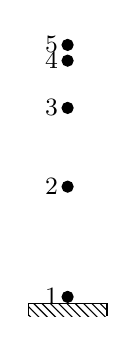
\begin{tikzpicture}
  \filldraw [color=black] (0,0) node [anchor=east] {\small 1} circle [radius=2pt]; 
  \filldraw [color=black] (0,1.4) node [anchor=east] {\small 2} circle [radius=2pt]; 
  \filldraw [color=black] (0,2.4) node [anchor=east] {\small 3} circle [radius=2pt]; 
  \filldraw [color=black] (0,3) node [anchor=east] {\small 4} circle [radius=2pt]; 
  \filldraw [color=black] (0,3.2) node [anchor=east] {\small 5} circle [radius=2pt]; 
  \draw [pattern=north west lines] (-0.5,-7pt)--(-0.5,-2.5pt)--(0.5,-2.5pt)--(0.5,-7pt);
\end{tikzpicture}
:>
所示不计空气阻力.求此屋檐离地面的高度及滴水的时间间隔.($g$取$10m/s^2$)

a.屋檐离地面高度为$3.2m$ ,滴水的时间间隔为$0.2s$

e.记第3滴和第2滴水滴的高度差为$\Delta h$ ,设滴水的时间间隔为$T$ ,则
法一:计算出第5滴水到第3滴水的距离和第5滴水到第2滴水的距离,二者的差就是窗户的高度了.即
$$\Delta h=\frac{1}{2}g(3T)^2-\frac{1}{2}g(2T)^2$$
解得
$$T=\sqrt{\frac{2\Delta h}{5g}}=0.2s$$
则屋檐离地面的高度$h$为
$$h=\frac{1}{2}g(4T)^2=3.2m$$

ee.法二:此题也可以借助于平均速度等于中间时刻的瞬时速度来解.由$\Delta h$ 可以计算出第2滴水滴和第3滴水滴之间的平均速度,此速度等于中间时刻$2.5T$ 的瞬时速度,即
$$\frac{\Delta h}{T}=g\cdot \frac{5}{2}T$$
解得
$$T=\sqrt{\frac{2\Delta h}{5g}}=0.2s$$
则屋檐离地面的高度$h$为
$$h=\frac{1}{2}g(4T)^2=3.2m$$

ee.法三:此题也可以借助初速度为零的比例式来求解.这四段距离之比为
$$1:3:5:7$$
所以第2滴水滴和第3滴水滴的距离占5份,而总共是$1+3+5+7=16$ 份,所以总的高度为
$$h=\frac{16}{5}\times 1m=3.2m$$
第5滴水滴到第4滴水滴的时间就是时间间隔$T$,即
$$\frac{1}{5}\Delta h=\frac{1}{2}gT^2$$
解得
$$T=\sqrt{\frac{2\Delta h}{5g}}=0.2s$$

16.A、B两辆汽车在笔直的公路上同向行驶.当B车在A车前$84m$处时,B 车的速度为$4m/s$,且正以$2m/s^2$的加速度做匀加速直线运动;经过一段时间后,B车的加速度突然变成零.A车一直以$20m/s$ 的速做匀速运动.经过$12s$后两车相遇.问B车加速行驶的时间是多少?

a.B车加速行驶的时间是$6s$

e.$12s$后A车的位移为
$$x_A=v_At_m=240m$$
则由于两车开始相距$84m$,所以B车的位移为
$$x_B=240m-84m=156m$$
设B车加速行驶的时间为$t$,则
$$x_B=v_{B0}t+\frac{1}{2}at^2+(v_{B0}+at)(t_m-t)$$
代入数值得关于时间的一元二次方程为
$$t^2-24t+108=0$$
采用十字相乘法得
$$(t-6)(t-18)=0$$
由于$t<12s$所以解得B车加速行驶的时间为
$$t=6s$$

16.利用水滴下落可以测出重力加速度$g$,调节水龙头,让水一滴一滴地流出,在水龙头的正下方放一个盘子,调整盘子的高度,使一个水滴碰到盘子时,恰好有一滴从水龙头开始下落,而空中还有一个正在下落的水滴,测出水龙头到盘子的距离为$h$,再从第一滴离开水龙头开始计时,到第$N$滴落到盘中,测出共用时间为$t$,求
[1]当第一滴落到盘子时,第二滴水滴离开水龙头的距离为多少?
[2]两滴水间的时间间隔是多少?
[3]重力加速度$g$是多大?

a.见解析

e.(1)利用初速度为零的匀变速直线运动的比例关系可得,第二滴水离开水龙头的距离与第一滴水离开水龙头的距离之比为$1:4$,所以第二滴水滴离开水龙头的距离为$\frac{h}{4}$

ee.(2)如<:
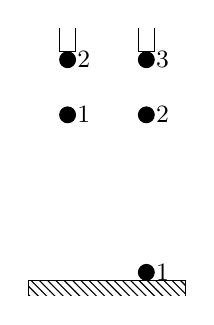
\begin{tikzpicture}
  \draw [pattern=north west lines] (-1,-0.2)--(-1,0)--(1,0)--(1,-0.2);
  \draw (-0.6,3.2)--(-0.6,2.9)--(-0.4,2.9)--(-0.4,3.2);
  \filldraw [color=black] (-0.5,2.8) circle [radius=1mm];
  \draw (-0.5,2.8) node [anchor=west] {\small $2$};
  \filldraw [color=black] (-0.5,2.1) circle [radius=1mm];
  \draw (-0.5,2.1) node [anchor=west] {\small $1$};
  \draw (0.6,3.2)--(0.6,2.9)--(0.4,2.9)--(0.4,3.2);
  \filldraw [color=black] (0.5,2.8) circle [radius=1mm];
  \draw (0.5,2.8) node [anchor=west] {\small $3$};
  \filldraw [color=black] (0.5,2.1) circle [radius=1mm];
  \draw (0.5,2.1) node [anchor=west] {\small $2$};
  \filldraw[color=black] (0.5,0.1) circle [radius=0.1];
  \draw (0.5,0.1) node [anchor=west] {\small $1$};
\end{tikzpicture}
:>所示,设两滴水滴下落间隔为$T$,其中第一滴下落到盘中所需时间为$2T$,再过$T$第二滴水下落到盘中,而之前第二滴水的位置已经被第三滴水占据,所以再过$T$第三滴水落到盘中,因此以后每隔一个$T$就有一滴水落到盘中,则第一滴水之后一共有$N-1$滴水滴,所以总时间为
$$2T+(N-1)T=t$$
解得,两滴水间的时间间隔是
$$\frac{t}{N+1}$$

ee.上面的这个情况还可以推广,如果空中有$m$个水滴,则第一滴水下落到盘中需要$m+1$个$T$,之后每个$T$就有一个水滴落入盘中,所以总时间为$(m+1)T+(N-1)T=(N+m)T$,因此$T$为
$$T=\frac{t}{N+m}$$

ee.(3)第一个$T$内水滴下落的距离已经由第(1)问求出,由自由落体位移与时间的关系得
$$\frac{h}{4}=\frac{1}{2}gT^2$$
解得
$$g=\frac{h}{2T^2}$$
将(2)中计算的时间间隔代入上式得
$$g=\frac{h(N+1)^2}{2t^2}$$

\end{calculate}



\subsection{逐差法求加速度}
我们首先说明为什么要用逐差法来处理问题,因为实验有误差,我们处理的原则是让误差尽可能小.一般毫米刻度尺的绝对误差是$1mm$,如图\ref{fig:rulemm}所示
\begin{figure}[H]
  \centering
  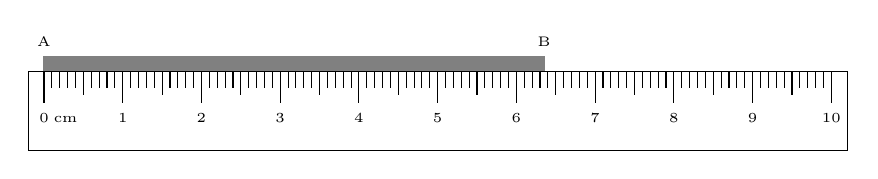
\begin{tikzpicture}
    \foreach \x in {
      0.1,0.2,0.3,0.4,0.6,0.7,0.8,0.9,
      1.1,1.2,1.3,1.4,1.6,1.7,1.8,1.9,
      2.1,2.2,2.3,2.4,2.6,2.7,2.8,2.9,
      3.1,3.2,3.3,3.4,3.6,3.7,3.8,3.9,
      4.1,4.2,4.3,4.4,4.6,4.7,4.8,4.9,
      5.1,5.2,5.3,5.4,5.6,5.7,5.8,5.9,
      6.1,6.2,6.3,6.4,6.6,6.7,6.8,6.9,
      7.1,7.2,7.3,7.4,7.6,7.7,7.8,7.9,
      8.1,8.2,8.3,8.4,8.6,8.7,8.8,8.9,
      9.1,9.2,9.3,9.4,9.6,9.7,9.8,9.9,
    }
    \draw (\x,0)--(\x,-0.2);
    \foreach \y in {0,1,2,3,4,5,6,7,8,9,10}
    \draw (\y,0)--(\y,-0.4) node [anchor=north]{\tiny \y};
    \foreach \z in {0.5,1.5,2.5,3.5,4.5,5.5,6.5,7.5,8.5,9.5}
    \draw (\z,0)--(\z,-0.3);
    \draw (-0.2,0) rectangle (10.2,-1);
    \draw (0,-0.6) node [anchor=west]{\tiny cm};
    \filldraw [color=gray] (0,0.02) rectangle (6.35,0.2);
    \draw (0,0.2) node [anchor=south]{\tiny A};
    \draw (6.35,0.2) node [anchor=south]{\tiny B};
  \end{tikzpicture}
  \caption{毫米刻度尺绝对误差}
  \label{fig:rulemm}
\end{figure}

在图\ref{fig:rulemm}中,测量一个杆的长度,使$A$ 端与零刻度线对齐,然后读$B$ 端的读数就是杆的长度.但是$B$不是完全与某一个刻度线对齐的,仔细观察不难发现它是一个介于$6.3mm$ 和$6.4mm$的数,所以坐标$x_B$ 的读数误差最大也就是$6.4mm-6.3mm=1mm$.对于一条纸带,我们在测量距离时,如图\ref{fig:zhidai}所示

\begin{figure}[H]
  \centering
  \begin{tikzpicture}
    \foreach \x in {
      0.1,0.2,0.3,0.4,0.6,0.7,0.8,0.9,
      1.1,1.2,1.3,1.4,1.6,1.7,1.8,1.9,
      2.1,2.2,2.3,2.4,2.6,2.7,2.8,2.9,
      3.1,3.2,3.3,3.4,3.6,3.7,3.8,3.9,
      4.1,4.2,4.3,4.4,4.6,4.7,4.8,4.9,
      5.1,5.2,5.3,5.4,5.6,5.7,5.8,5.9,
      6.1,6.2,6.3,6.4,6.6,6.7,6.8,6.9,
      7.1,7.2,7.3,7.4,7.6,7.7,7.8,7.9,
      8.1,8.2,8.3,8.4,8.6,8.7,8.8,8.9,
      9.1,9.2,9.3,9.4,9.6,9.7,9.8,9.9,
    }
    \draw (\x,0)--(\x,-0.2);
    \foreach \y in {0,1,2,3,4,5,6,7,8,9,10}
    \draw (\y,0)--(\y,-0.4) node [anchor=north]{\tiny \y};
    \foreach \z in {0.5,1.5,2.5,3.5,4.5,5.5,6.5,7.5,8.5,9.5}
    \draw (\z,0)--(\z,-0.3);
    \draw (-0.2,0) rectangle (10.2,-1);
    \draw (0,-0.6) node [anchor=west]{\tiny cm};
    \draw (-0.2,-0.4)--(-0.4,-0.4)--(-0.4,0.5)--(10.4,0.5)--(10.4,-0.4)--(10.2,-0.4);
    \foreach \x in {0,0.2,0.8,1.8,3.2,5,7.2,9.8}
    \filldraw [color=black] (\x , 0.05) circle [radius=1pt];
    \foreach \x in {0,0.2,0.8,1.8,3.2,5,7.2,9.8}
    \draw (\x , 0.05) node [anchor=south] {\tiny \thepointnum\stepcounter{pointnum}};
  \end{tikzpicture}
  \caption{测量纸带上点的距离}
  \label{fig:zhidai}
\end{figure}

在图\ref{fig:zhidai}中,使纸带上的计数点$0$ 与刻度尺上的零刻度对齐,然后依次读取其它点的读数,这些读数记作$x_i' \quad (i=0,1,2 \cdots)$,在纸带上标出这些读数如\ref{fig:zhidaidushu}所示

\setcounter{pointnum}{0}
\begin{figure}[H]
  \centering
  \begin{tikzpicture}
    \draw (-0.4,-0.4) rectangle (10.4,0.5); 
    \foreach \x in {0,0.2,0.8,1.8,3.2,5,7.2,9.8}
    \filldraw [color=black] (\x , 0.05) circle [radius=1pt];
    \foreach \x in {0,0.2,0.8,1.8,3.2,5,7.2,9.8}
    \draw (\x , 0.05) node [anchor=south] {\tiny \thepointnum\stepcounter{pointnum}};
    \draw (0,0)--(0,-0.8);
    \draw (0.2,0)--(0.2,-0.15);
    \draw [->,>=stealth] (0,-0.1)--(0.2,-0.1) ;
    \draw (0.2,-0.15) node {\tiny $x_1'$};
    \draw (0.8,0)--(0.8,-0.25);
    \draw [->,>=stealth] (0,-0.2)--(0.8,-0.2); 
    \draw (0.8,-0.3) node [anchor=south east] {\tiny $x_2'$};
    \draw (1.8,0)--(1.8,-0.35);
    \draw [->,>=stealth] (0,-0.3)--(1.8,-0.3) node [anchor=south east] {\tiny $x_3'$};
    \draw (3.2,0)--(3.2,-0.45);
    \draw [->,>=stealth] (0,-0.4)--(3.2,-0.4)node [anchor=south east] {\tiny $x_4'$};
    \draw (5,0)--(5,-0.55);
    \draw [->,>=stealth] (0,-0.5)--(5,-0.5)node [anchor=south east] {\tiny $x_5'$};
    \draw (7.2,0)--(7.2,-0.65);
    \draw [->,>=stealth] (0,-0.6)--(7.2,-0.6)node [anchor=south east] {\tiny $x_6'$};
    \draw (9.8,0)--(9.8,-0.75);
    \draw [->,>=stealth] (0,-0.7)--(9.8,-0.7)node [anchor=south east] {\tiny $x_7'$};
  \end{tikzpicture}
  \caption{计数点的读数标记}
  \label{fig:zhidaidushu}
\end{figure}

我们以不带撇号的坐标表示两点间的距离,如图\ref{fig:zhidaijvli}所示

\setcounter{pointnum}{0}
\begin{figure}[H]
  \centering
  \begin{tikzpicture}
    \draw (-0.4,-0.4) rectangle (10.4,0.5); 
    \foreach \x in {0,0.2,0.8,1.8,3.2,5,7.2,9.8}
    \filldraw [color=black] (\x , 0.05) circle [radius=1pt];
    \foreach \x in {0,0.2,0.8,1.8,3.2,5,7.2,9.8}
    \draw (\x , 0.05) node [anchor=south] {\tiny \thepointnum\stepcounter{pointnum}};
    \draw [<-,>=stealth] (0.2,0.05)--(0.4,0.05);
    \draw (0.5,0.05) node {\tiny $x_2$};
    \draw [->,>=stealth] (0.6,0.05)--(0.8,0.05);
    \draw [<-,>=stealth] (0.8,0.05)--(1.15,0.05);
    \draw (1.3,0.05) node {\tiny $x_3$};
    \draw [->,>=stealth] (1.45,0.05)--(1.8,0.05);
    \draw [<-,>=stealth] (1.8,0.05)--(2.35,0.05);
    \draw (2.5,0.05) node {\tiny $x_4$};
    \draw [->,>=stealth] (2.65,0.05)--(3.2,0.05);
    \draw [<-,>=stealth] (3.2,0.05)--(3.95,0.05);
    \draw (4.1,0.05) node {\tiny $x_5$};
    \draw [->,>=stealth] (4.25,0.05)--(5,0.05);
    \draw [<-,>=stealth] (5,0.05)--(5.95,0.05);
    \draw (6.1,0.05) node {\tiny $x_6$};
    \draw [->,>=stealth] (6.25,0.05)--(7.2,0.05);
    \draw [<-,>=stealth] (7.2,0.05)--(8.35,0.05);
    \draw (8.5,0.05) node {\tiny $x_7$};
    \draw [->,>=stealth] (8.65,0.05)--(9.8,0.05);
  \end{tikzpicture}
  \caption{计数点的距离标记}
  \label{fig:zhidaijvli}
\end{figure}

由于我在这里作图是按照标准的$1:3:5:7:9:11$ 完成的,第一段的距离太小,为了防止第一段看不清楚,所以在第一段上没有标出$x_1$,同时由图 \ref{fig:zhidaidushu}和图\ref{fig:zhidaijvli}对比可知两种表示方法的关系为

\begin{equation}
  x_i=x_i'-x_{i-1}' \qquad (i=1,2,3 \cdots)
  \label{eq:dushujvli}
\end{equation}

下面我们讨论加速度的计算,由$x_2$ 和$x_1$ 我们可以计算加速度,如下
\begin{gather}
  x_2-x_1=a_1T^2
  \intertext{经过简单计算可得}
  a_1=\frac{x_2-x_1}{T^2}
  \intertext{同理也可以得到加速度}
  a_2=\frac{x_3-x_2}{T^2}\\
  a_3=\frac{x_4-x_3}{T^2}\\
  a_4=\frac{x_5-x_4}{T^2}
  \intertext{由于在$a_1$的分子部分需要三个坐标来确定这个差,所以它的误差为$3mm$,$a_2$和$a_3$需要四个坐标来确定分子部分的差,所以其误差为$4mm$,但$T$是相同的,下面我们将这四个加速度取几何平均,则得到}
  a_{1234}=\frac{1}{4}(a_1+a_2+a_3+a_4)=\frac{x_5-x_1}{4T^2}
  \intertext{上面这个平均加速度,其分子部分需要三个坐标确定,但是分子上需要除以$4$,所以它的误差为$3mm/4=0.75mm$,同理我们可以得到$a_{2345}$等类似的平均值,如下}
  a_{2345}=\frac{1}{4}(a_2+a_3+a_4+a_5)=\frac{x_6-x_2}{4T^2}\\
  a_{3456}=\frac{1}{4}(a_3+a_4+a_5+a_6)=\frac{x_7-x_3}{4T^2}
  \intertext{上面的$a_{2345}$和$a_{3456}$的分子部分需要4个坐标确定,所以它们的误差是$4mm/4=1mm$,但是如果再取一次平均,如下}
  a=\frac{1}{3}(a_{1234}+a_{2345}+a_{3456})=\frac{(x_5+x_6+x_7)-(x_1+x_2+x_3)}{3\times 4T^2}
  \intertext{上式分子部分等于$x_7'-x_4'-x_3'$,用到了三个读数,但是分母上需要除以$12$ 所以它的误差是$3mm/12=0.25mm$,所以最后这个结果误差是最小的,为我们所采纳,这就是逐差法公式.下面我们总结写出加速度的方法,分母上的这个数值可以这样来确定:分子中的括号中有$3$个数值,同时每个数值的下标差相同(比如$5-1=4$,$6-2=4$,$7-3=4$),分母上的这个数值就是$3\times4=12$,同理我们可以写出$6$段和$9$段的计算公式如下}
  a=\frac{(x_4+x_5+x_6)-(x_1+x_2+x_3)}{3\times3 T^2}\\
  a=\frac{(x_6+x_7+x_8+x_9)-(x_1+x_2+x_3+x_4)}{4\times5 T^2}
  \intertext{有许多人为了方便记住逐差法的公式,在偶数段时将纸带一分为二,比如$6$段时,可以写作}
  a=\frac{(x_4+x_5+x_6)-(x_1+x_2+x_3)}{(3T)^2}
  \intertext{这可以理解为时间间隔为$3T$ 的两大段,使用$\Delta x=aT^2$ 一步写出,但是在遇到奇数段(比如$7$段)的时候就会遇到麻烦,如果按这个逻辑,可以选用前$6$段或者后$6$段,这样写出的公式误差是$3mm/9=0.33mm$,而按逐差法写出的公式是\CJKunderwave{去掉中间一段}这样计算的结果误差为$3mm/12=0.25mm$,显然\CJKunderwave{去掉中间一段}才能得到更精确的答案.}
  \notag
\end{gather}
\subsection{习题精解二}
\begin{calculate}
11.一滴雨滴从离地面 $20m$ 高的楼房屋檐自由下落,下落过程中用 $0.2s$ 的时间通过一个窗口,窗口的高度为 $2m$ , $g$ 取 $10m/s^2$ ,问:
[1]雨滴落地时的速度大小;
[2]雨滴落地前最后 $1s$ 内的位移大小;
[3]屋檐离地面的上边框有多高?

a.见解析

e.(1)由匀变速直线运动速度与位移的关系可得
$$v^2=2gh \Longrightarrow v=\sqrt{2gh}=20m/s$$

ee.(2)法一:雨滴在最后$1s$内的平均速度等于中间时刻的瞬时速度,中间时刻到最后共经历 $t_1=0.5s$ 所以有
$$v=\overline{v}+gt_1 \Longrightarrow \overline{v}=v-gt_1=15m/s$$
由位移等于平均速度乘以时间得
$$\Delta h=\overline{v}\Delta t_1 =15m$$

ee.法二:仍然采用平均速度的方法,先求出总时间,然后再求出最后$1s$的中间时刻,即
$$h=\frac{1}{2}gt^2 \Longrightarrow t=\sqrt{\frac{2h}{g}}=2s$$
所以最后$1s$ 的中间时刻即 $t=1.5s$ 时瞬时速度等于平均速度
$$\overline{v}=gt=15m/s$$
由位移等于平均速度乘以时间得
$$\Delta h=\overline{v}\Delta t_1 =15m$$

ee.法三:先求出总时间,然后再算出前 $1s$ 的时刻,并求出位移和总位移作差也可以得到最后 $1s$ 内的位移.即
$$h=\frac{1}{2}gt^2 \Longrightarrow t=\sqrt{\frac{2h}{g}}=2s$$
从下落开始到落地前$1s$经历的时间为$t_1=1s$ ,所以
$$h_1=\frac{1}{2}gt_1^2=5m$$
最后$1s$ 内的位移为
$$\Delta h=h-h_1=20m-5m=15m$$


ee.(3)在雨滴通过窗口的过程中,用时$0.2s$,所以它的中间时刻的瞬时速度等于平均速度为
$$\overline{v'}=\frac{2m}{0.2s}=10m/s$$
所以雨滴由屋檐到通过窗口的中间时刻所用时间为
$$t_0=\frac{\overline{v'}}{g}=1s$$
由此可得,雨滴由屋檐到窗口的时间为$t'=1s-0.1s=0.9s$ 所以屋檐离窗口上边框的高度为
$$h'=\frac{1}{2}gt'^2=4.05m$$

12.一辆值勤的警车停在公路边,当警员发现从他旁边以$10m/s$ 的速度匀速行驶的货车严重超载时,决定前去追赶,经过$5.5s$ 后警车发动起来,并以$2.5m/s^2$的加速度做匀加速运动,但警车的行驶速度必须控制在$90km/h$以内,问:
[1]警车在追赶货车的过程中,两车的最大距离是多少?
[2]警车发动后要经过多长时间 才能追上货车?

a.(1) 75m \qquad (2) 12s

e.(1)以警车发动起来作为计时起点,首先将警车的最大速度切换成国际单位 $90km/h=25m/s$ ,则警车的加速过程的持续时间$t_m$ 为
$$v_m=at_m \Longrightarrow t_m=\frac{v_m}{a}=10s$$
写出$0\sim 10s$ 内两车的距离为
$$\Delta x=55+10t -\frac{5}{4}t^2$$
整理成标准一元二次方程
$$\Delta x =-\frac{5}{4}t^2+10t+55 \quad (m)$$
由二次函数的知识,易得在$0\sim 10s$内 $t=4s$ 时距离最大,为
$$\Delta x_{max}=75m$$

ee.注意,在警车追赶货车的过程中,要分两步考虑,在$0\sim 10s$ 内,两车的距离关系才是上述的一元二次函数,但是这个过程不一定就追上,所以不能直接使用$\Delta x=0$ 来计算出时间,这就导致错误了!! 最好的方法就是画出这段时间内的函数图象,然后得出能否在 $10s$ 内追上的明确结论.容易得到 $t=10s$ 时
$$\Delta x'=-\frac{5}{4}\times 10^2 +100 +55m =30m$$
于是加速过程结束时,警车没有追上货车,所以还要匀速追一段时间$t'$ 所以
$$t'=\cfrac{\Delta x'}{v_2-v_1}=2s$$
则警车追赶货车共用时间为
$$t=t_m+t'=12s$$

13.某人骑自行车以$v_1=4m/s$ 的速度前进,某时刻在他前面$x_0=7m$ 处有以$v_1=10m/s$ 的速度同向行驶的汽车开始关闭发动机减速前进,而以$a=-2m/s^2$ 的加速度匀减速前进,求:
[1]此人追上汽车之前落后于汽车的最大距离?
[2]此人需要多长时间才能追上汽车?

a.(1) 16m \qquad (2) 8s

e.(1)此问题出现了刹车,所以先求出刹车时间$t_s$
$$0=v_0+at_s \Longrightarrow t_s=-\frac{v_0}{a}=5s$$
容易写出$0\sim 5s$ 内两车的距离为
$$\Delta x = (7+10t-t^2)-4t $$
化成标准形式
$$\Delta x=-t^2+6t+7 \quad (m)$$
由一元二次方程得$t=3s$ 时,二者距离最大为
$$\Delta x_{max}=16m$$

ee.(2)注意,只有在$0\sim 5s$ 内二者的距离才按上述方程变化,但是不能保证$5s$ 内一定能追上,这需要单独判断.易得$t=5s$ 时,二者距离为
$$\Delta x'=-5^2+6\times 5 +7 m =12m$$
在$5s$时,人还没有追上汽车,而这时汽车已经停止运动,所以剩下的这$12m$ 人需要匀速追击,其所需时间$t'$ 为
$$t'=\frac{\Delta x'}{v_1}=3s$$
所以人追车的总时间为
$$t=t_s+t'=8s$$


14.甲、乙两车从\CJKunderwave{同一地点}出发,同向运动,其$v-t$ 图象如
<:
\begin{tikzpicture}
  \draw[->] (0,0)--(0,2.2) node [anchor=west]{\tiny $v/m\cdot s^{-1}$}; 
  \draw[->] (0,0)--(2.5,0) node [anchor= north]{\tiny $t/s$};
  \draw (0.5,0) node [anchor=north] {\tiny $2$};
  \draw (1,0) node [anchor=north] {\tiny $4$};
  \draw (1.5,0) node [anchor=north] {\tiny $6$};
  \draw (2,0) node [anchor=north] {\tiny $8$};
  \draw (0,0.3) node [anchor=east]{\tiny $1$};
  \draw (0,0.6) node [anchor=east]{\tiny $2$};
  \draw (0,0.9) node [anchor=east]{\tiny $3$};
  \draw (0,1.2) node [anchor=east]{\tiny $4$};
  \draw (0,1.5) node [anchor=east]{\tiny $5$};
  \draw (0,0)--(1,0.9)--(1.5,1.35);
  \draw (0.5,0)--(1,0.9)--(1.5,1.8);
  \draw[dotted] (1,0.9)--(0,0.9);
  \draw[dotted] (1,0.9)--(1,0);
  \draw[dotted] (1.5,0)--(1.5,1.85);
  \draw (1.5,1.35) node [anchor=north] {\tiny 甲};
  \draw (1.5,1.85) node [anchor=east] {\tiny 乙};
\end{tikzpicture}
:>所示.试计算:
[1]甲乙两车的加速度各为多大?
[2]两车相遇前的最大距离为多少?
[3]从乙车开始运动起经过多长时间后两车相遇?(计算结果保留$2$位小数)

a.(1) $a_{\mbox{\tiny 甲}}=\frac{3}{4}m/s^2$ \qquad $a_{\mbox{\tiny 乙}}=\frac{3}{2}m/s^2$ \qquad (2) $3m$ \qquad (3) $4.83s$

e.(1)由加速度的定义根据图象易得,计算从略.

ee.(2)如<:
\begin{tikzpicture}
  \draw[->] (0,0)--(0,2.2) node [anchor=west]{\tiny $v/m\cdot s^{-1}$}; 
  \draw[->] (0,0)--(2.5,0) node [anchor= north]{\tiny $t/s$};
  \draw (0.5,0) node [anchor=north] {\tiny $2$};
  \draw (1,0) node [anchor=north] {\tiny $4$};
  \draw (1.5,0) node [anchor=north] {\tiny $6$};
  \draw (2,0) node [anchor=north] {\tiny $8$};
  \draw (0,0.3) node [anchor=east]{\tiny $1$};
  \draw (0,0.6) node [anchor=east]{\tiny $2$};
  \draw (0,0.9) node [anchor=east]{\tiny $3$};
  \draw (0,1.2) node [anchor=east]{\tiny $4$};
  \draw (0,1.5) node [anchor=east]{\tiny $5$};
  \draw (0,0)--(1,0.9)--(1.5,1.35);
  \draw (0.5,0)--(1,0.9)--(1.5,1.8);
  \draw[dotted] (1,0.9)--(0,0.9);
  \draw[dotted] (1,0.9)--(1,0);
  \draw[dotted] (1.5,0)--(1.5,1.85);
  \draw (1.5,1.35) node [anchor=north] {\tiny 甲};
  \draw (1.5,1.85) node [anchor=east] {\tiny 乙};
  \draw [pattern=north west lines] (0,0)--(1,0.9)--(0.5,0);
\end{tikzpicture}
:>所示,由于$v-t$图象与$t$轴所围图形的面积表示位移,同时两车又是从\CJKunderwave{同一位置}开始运动,则开始时甲比乙快,所以甲比乙领先,于是两车位移差就是它们的距离,对应图中所示阴影面积就是两车的最大距离.即
$$\Delta x_{max}=\frac{1}{2}\times 2\times 3 m=3m$$

ee.(3)两车的距离随时间变化的规律容易得到,即
$$\Delta x=\frac{1}{2}a_{\mbox{\tiny 甲}}(t+2)^2-\frac{1}{2}a_{\mbox{\tiny 乙}}t^2$$
令$\Delta x =0$ 得
$$(\frac{t+2}{t})^2=\cfrac{a_{\mbox{\tiny 乙}}}{\mbox{\tiny 甲}}=2$$
解得$t=2(\sqrt{2}+1)s$ 由于题目中要求保留$2$位小数,所以取为
$$t=2(\sqrt{2}+1)s\approx 4.83s$$
{\bf 注意}使用速度时间图象法可以确定两车的最大距离,但是应该特别注意这点在{\bf 两车初始时刻位于同一位置}时才可行,如果\CJKunderwave{不是同一位置}则还是应该列出具体方程来讨论它们之间的距离随时间的变化才行,因此这属于一种特殊情况.

15.屋檐第隔相同的时间间隔滴下一滴水,当第$5$滴正欲下时,第$1$滴刚好到地面,而第$3$滴与第$2$滴分别位于高为 $1$米的窗子的上、下沿,如
<:
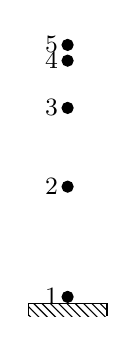
\begin{tikzpicture}
  \filldraw [color=black] (0,0) node [anchor=east] {\small 1} circle [radius=2pt]; 
  \filldraw [color=black] (0,1.4) node [anchor=east] {\small 2} circle [radius=2pt]; 
  \filldraw [color=black] (0,2.4) node [anchor=east] {\small 3} circle [radius=2pt]; 
  \filldraw [color=black] (0,3) node [anchor=east] {\small 4} circle [radius=2pt]; 
  \filldraw [color=black] (0,3.2) node [anchor=east] {\small 5} circle [radius=2pt]; 
  \draw [pattern=north west lines] (-0.5,-7pt)--(-0.5,-2.5pt)--(0.5,-2.5pt)--(0.5,-7pt);
\end{tikzpicture}
:>
所示不计空气阻力.求此屋檐离地面的高度及滴水的时间间隔.($g$取$10m/s^2$)

a.屋檐离地面高度为$3.2m$ ,滴水的时间间隔为$0.2s$

e.记第3滴和第2滴水滴的高度差为$\Delta h$ ,设滴水的时间间隔为$T$ ,则
法一:计算出第5滴水到第3滴水的距离和第5滴水到第2滴水的距离,二者的差就是窗户的高度了.即
$$\Delta h=\frac{1}{2}g(3T)^2-\frac{1}{2}g(2T)^2$$
解得
$$T=\sqrt{\frac{2\Delta h}{5g}}=0.2s$$
则屋檐离地面的高度$h$为
$$h=\frac{1}{2}g(4T)^2=3.2m$$

ee.法二:此题也可以借助于平均速度等于中间时刻的瞬时速度来解.由$\Delta h$ 可以计算出第2滴水滴和第3滴水滴之间的平均速度,此速度等于中间时刻$2.5T$ 的瞬时速度,即
$$\frac{\Delta h}{T}=g\cdot \frac{5}{2}T$$
解得
$$T=\sqrt{\frac{2\Delta h}{5g}}=0.2s$$
则屋檐离地面的高度$h$为
$$h=\frac{1}{2}g(4T)^2=3.2m$$

ee.法三:此题也可以借助初速度为零的比例式来求解.这四段距离之比为
$$1:3:5:7$$
所以第2滴水滴和第3滴水滴的距离占5份,而总共是$1+3+5+7=16$ 份,所以总的高度为
$$h=\frac{16}{5}\times 1m=3.2m$$
第5滴水滴到第4滴水滴的时间就是时间间隔$T$,即
$$\frac{1}{5}\Delta h=\frac{1}{2}gT^2$$
解得
$$T=\sqrt{\frac{2\Delta h}{5g}}=0.2s$$

\end{calculate}

  \chapter{相互作用}
  \section{力\quad 基本相互作用}
\subsection{定义}
物体与物体的\CJKunderwave{相互作用}叫做力.英文中力是Force ,所以力的符号用 F 表示.

基本相互作用(fundamental interaction),为物质间最基本的相互作用,常称为{\heiti 自然界四力}或{\heiti 宇宙基本力}.迄今为止观察到的所有关于物质的物理现象,在物理学中都可以借肋这四种基本相互作用的机制得到描述和解释.\footnote{引用自百度百科词条:基本相互作用}

\subsubsection{万有引力}

万有引力是四个基本相互作用中最弱的,但是同时又是作用范围最大的,当距离增大时,万有引力作用将会递减,假设两个质点相距$r$,其质量分别为$m_1,m_2$,则万有引力的计算公式为
\begin{equation}
  F=G\cfrac{m_1m_2}{r^2}
\end{equation}

\subsubsection{弱相互作用}

弱相互作用又叫做弱核力,次原子粒子的放射性衰变就是由它引起的,恒星中一种叫做氢聚变的过程也是由它启动的.弱相互作用会影响所有的费米子,即所有自旋为半奇数的粒子.主要是核子产生天然放射,四种基本相互作用中,弱相互作用只比万有引力强一点.

\subsubsection{电磁相互作用}

世界上大部分物质都具有电磁力,而磁与电是电磁力的不同表现模式,本质上是相同的一种物质.例如:电荷异性相吸,同性相斥的特性就是其中之一,电磁力和重力一样,其作用影响范围是无限大的.

\subsubsection{强相互作用}
强相互作用又称为强核力,所有存在宇宙中的物体都是由原子构成的,而原子又是由原子核与核外电子构成的,原子核由中子和质子组成.中子没有电荷,而质子带正电,但需要牵引力把它们结合在一起,强相互作用就是这种``牵引力''.

\subsection{力的性质}
\subsubsection{矢标性}
力是也有大小和方向,同时力的计算满足平行四边行定则,所以力是一个矢量.
\subsubsection{单位}
为了纪念伟大的物理学家牛顿在力学中的贡献,将力的单位定为:牛顿,简称:牛,符号:$N$
\subsubsection{力的作用效果}
力的作用效果有两种:一,使物体的\CJKunderwave{运动状态}发生变化;二,使物体\CJKunderwave{发生形变}.
\subsubsection{注意事项}
物体与物体有相互作用,不一定要直接相互接触.例如:电荷与电荷之间,磁体与磁体之间,磁体与电流之间,地球与太阳之间,都有相互作用,但是都没有直接接触.

\subsection{力的示意图}
力有三个基本要素:\CJKunderwave{大小}、\CJKunderwave{方向}、\CJKunderwave{作用点}.

严格来讲,力还有作用线,它会影响到物体的力矩和转动效应,但是这一部分主要研究平动,不涉及转动,所以暂时不研究作用线.

在处理问题时,有时不必把力的三个基本要素都画出来,这里只画出力的方向和作用点就可以了,这样\CJKunderwave{用一条带箭头的线段(有向线段)来表示力}的方向,叫做力的示意图.注意,此时不必标注力的大小.

如图\ref{fig:shiyitu} 给出了力的示意图的一个示例,其中作用点既可以画作前头处,也可以画在前尾处.
\begin{figure}[H]
  \centering
  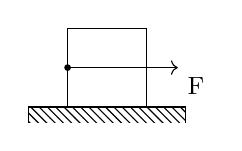
\begin{tikzpicture}
    \draw (0,0) rectangle (1,1);
    \draw [pattern=north west lines](-0.5,-0.2)--(-0.5,0)--(1.5,0)--(1.5,-0.2);
    \draw [->] (0,0.5) -- (1.4,0.5) node [anchor=north west]{\small F};
    \filldraw[black] (0,0.5) circle [radius=1pt];
  \end{tikzpicture}
  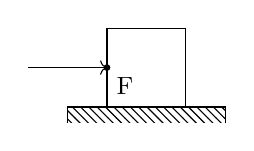
\begin{tikzpicture}
    \draw (0,0) rectangle (1,1);
    \draw [pattern=north west lines](-0.5,-0.2)--(-0.5,0)--(1.5,0)--(1.5,-0.2);
    \draw [->] (-1,0.5) -- (0,0.5) node [anchor=north west]{\small F};
    \filldraw[black] (0,0.5) circle [radius=1pt];
  \end{tikzpicture}
  \caption{力的示意图}
  \label{fig:shiyitu}
\end{figure}
\subsubsection{力的图示}
力的图示就是用作图的方式表示力,这就要求表示出力的大小、方向和作用点.所以作力的图示,首先要根据所画力的大小选择适当的单位长度.仍然是用一条带箭头的线段(有向线段)来表示力,线段的长度表示力的大小,作用点和方向同力的示意图.
 
如图\ref{fig:tushi} 所示画出了一个$15N$ 的拉力 和 一个 $8N$ 的推力.

\begin{figure}[H]
  \centering
  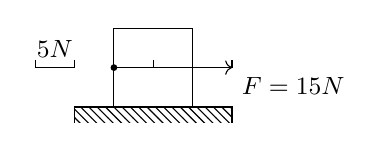
\begin{tikzpicture}
    \draw (-1,0.5)--(-0.5,0.5);
    \draw (-1,0.5)--(-1,0.6);
    \draw (-0.5,0.5)--(-0.5,0.6);
    \draw (-0.75,0.5) node [anchor=south] {\small $5N$};
    \draw (0,0) rectangle (1,1);
    \draw [pattern=north west lines](-0.5,-0.2)--(-0.5,0)--(1.5,0)--(1.5,-0.2);
    \draw [->] (0,0.5) -- (1.5,0.5) node [anchor=north west]{\small $F=15N$};
    \draw (0,0.5)--(0,0.6);
    \draw (0.5,0.5)--(0.5,0.6);
    \draw (1,0.5)--(1,0.6);
    \draw (1.5,0.5)--(1.5,0.6);
    \filldraw[black] (0,0.5) circle [radius=1pt];
  \end{tikzpicture}
  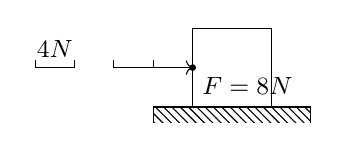
\begin{tikzpicture}
    \draw (-2,0.5)--(-1.5,0.5);
    \draw (-2,0.5)--(-2,0.6);
    \draw (-1.5,0.5)--(-1.5,0.6);
    \draw (-1.75,0.5) node [anchor=south] {\small $4N$};
    \draw (0,0) rectangle (1,1);
    \draw [pattern=north west lines](-0.5,-0.2)--(-0.5,0)--(1.5,0)--(1.5,-0.2);
    \draw (-1,0.5)--(-1,0.6);
    \draw (-0.5,0.5)--(-0.5,0.6);
    \draw [->] (-1,0.5) -- (0,0.5) node [anchor=north west]{\small $F=8N$};
    \filldraw[black] (0,0.5) circle [radius=1pt];
  \end{tikzpicture}
  \caption{力的图示}
  \label{fig:tushi}
\end{figure}

\subsection{例题分析}

\begin{selection}
  1.关于力的概念,下列说法中正确的是
  A.力是使物体发生形变和运动状态发生变化的原因
  B.一个力必定联系着两个物体,其中每个物体既是施力物体也是受力物体
  C.只要两个力的大小相等,它们产生的效果一定相同
  D.两个物体相互作用,其相互作用力是有先后的

  a.AB

  e.从力的基本概念出发作出判断.根据力的两个作用效果,可知A正确.根据力的相互性,可知B正确.根据斩的三要素,可知力的作用效果不仅与力的大小有关,还与力的方向和作用点的位置有关,所以C错误.物体间的相互作用力是同时的,没有时间上的先后关系,所以D错误.关于相互作用的性质,在牛顿运动定律一节再进行深入讨论.

  2.下列说法正确的是
  A.``风吹草动'' ,草受到了力,但是没有施力物体,说明没有施力物体的力也是存在的
  B.运动员将球踢出,球在空中飞行是因为受到一个向前的推力
  C.甲用力把乙推倒,只是甲对乙有力,而乙对甲没有力
  D.两个物体发生相互作用不一定相互接触

  a.D

  e.力是物体对物体的作用,任何力都有施力物体和受力物体,它是一种客观实在,``风吹草动'',施力物体是空气,故A错.踢出去的球向前运动,是因为惯性,也可以认为没有找到施力物体,故而没有受到向前的推力,故B错.由力的相互性可知,甲推乙的同时,乙也推甲,故C错.物体发生相互作用并不一定相互接触,如电荷之间,磁铁之间的相互作用就不需要直接接触,D对.

\end{selection}

\begin{calculate}
  3.在图甲中木箱p点,用与水平方向成$30^\circ$角斜向上方的$150N$ 的力拉木箱;在图乙中木块的Q 点,用与竖直方向成$60^\circ$  角斜向左上方的$20N$ 的力把木块抵在墙壁上,试作出甲、乙两图中所给力的图示,并作出图丙中电灯所受重力和拉力的示意图.
  
\end{calculate}

\begin{figure}[H]
  \centering
  \begin{tikzpicture}
    \draw  (0,0) rectangle (1,1) node [anchor=north west]{\small $P$}; 
    \draw [pattern=north west lines](-0.5,-0.2)-- (-0.5 , 0)--(1.5,0)--(1.5,-0.2);
    \draw (0.5,-0.3) node [anchor=north]{\small 甲};
    \filldraw[black] (1,1) circle [radius=1pt];
    \draw (-1,0.5)--(-0.5,0.5);
    \draw (-1,0.5)--(-1,0.6);
    \draw (-0.5,0.5)--(-0.5,0.6);
    \draw (-0.75,0.6) node [anchor=south]{\tiny $50N$ };
    \draw [dotted] (1,1)--(2,1);
    \draw [->,rotate around={30:(1,1)}] (1,1)--(2.5,1) node [anchor=west]{\tiny $F=150N$};
    \draw [rotate around={30:(1,1)}](1.5,1)--(1.5,1.1);
    \draw [rotate around={30:(1,1)}](2,1)--(2,1.1);
    \draw [rotate around={30:(1,1)}](2.5,1)--(2.5,1.1);
    \draw [rotate around={25:(1,1)}](1.5,1) node [anchor=west]{\tiny $30^\circ$};
    \draw (1.4,1) arc (0:30:0.4);
  \end{tikzpicture}
  \begin{tikzpicture}
    \draw (0,0) rectangle (1,1) ;
    \draw (1,0) node [anchor=west] {\small $Q$};
    \filldraw[black] (1,0) circle [radius=1pt];
    \draw [pattern=north west lines](-0.2,1.3)--(0,1.3)--(0,-0.3)--(-0.2,-0.3);
    \draw (0.4,-0.3) node [anchor=north] {\small 乙};
    \draw [->,rotate around={60:(1,0)}] (1,0)--(1,1) node [anchor=south west]{\tiny $F=20N$};
    \draw [rotate around={60:(1,0)}] (1,0.5)--(1.1,0.5); 
    \draw (-1,0.5) -- (-0.5,0.5);
    \draw (-1,0.5) -- (-1,0.6);
    \draw (-0.5,0.5) -- (-0.5,0.6);
    \draw (-0.75,0.5) node [anchor=south] {\tiny $10N$};
    \draw (1,0.3) arc (90:150:0.3);
    \draw [rotate around={30:(1,0)}] (1,0.3) node [anchor=south]{\tiny $60^\circ$};
  \end{tikzpicture}
  \hspace{70pt}
  \begin{tikzpicture}
    \draw [pattern=north west lines] (-0.5,1)--(-0.5,0.8)--(0.5,0.8)--(0.5,1); 
    \draw (0,0.8)--(0,0);
    \draw (0,0)--(-0.4,-0.2)--(0.4,-0.2)--cycle;
    \draw (-0.2,-0.2) arc (180:360:0.2);
    \draw (0,-0.5) node [anchor=north] {\small 丙};
    \draw [->](0,-0.2)--(0,-1) node [anchor=west]{\tiny $G$};
    \draw [->](0,-0.2)--(0,0.6) node [anchor=west]{\tiny $T$};
    \filldraw [black] (0,-0.2) circle [radius=1pt];
  \end{tikzpicture}
\end{figure}

  \newpage
  \section{重力}
\subsubsection{定义}
由于\CJKunderwave{地球的吸引} 而使物体受到的力叫做重力.但是应当注意,地球对物体的吸引力不等价于重力,因为地球在自转,所以地球对物体的吸引力有两个作用,其一保持地球上的物体随地球一同绕地轴做匀速圆周运动(后面会讲到),其二,使物体下落.这个使物体下落的力叫做重力.地球对物体的吸引力叫做万有引力(后面会讲到),重力是万有引力的一个分力.

\subsubsection{计算式}
物体由于只受重力作用而产生的加速度叫做重力加速度,记作:$g=9.8m/s^2$.
则重力的大小为
$$G=mg$$

注意:由于后面会讲到万有引力,其表达式为$F=G\cfrac{m_1m_2}{r^2}$,它里面有一个$G$,所以在不引起误解的情况下表示重力一般用表达式$mg$. 同时,在初中时大家学过这个公式,其中$g$ 当时只说明是一个比例系数,同时单位是$N/kg$ ,容易说明 $N/kg=m/s^2$,这需要从牛顿第二定律(后面会讲到)来看.

\subsubsection{方向}
重力也是一个矢量,它的方向总是\CJKunderwave{竖直向下}.但是注意,竖直向下不是指向地心,万有引力的方向才指向地心,重力只是万有引力的一部分,所以不能说重力的方向是指向地心的.

\subsubsection{作用点}

物体的每一部分都受重力,但是在计算的时候可以找到一个等效作用点,即:认为物体所受重力作用点集中在一个点上,这个等效作用点就叫做重心.所以也可以说重力的作用点在重心上.计算重心要用到微积分,在高中阶段大家的数学水平尚不够充分,所以只要大家暂时记住会用便好.

根据计算,物体的重心取决于物体的质量分布、形状等因素,一个质量分布均匀、形状规则的物体,重心就是物体的几何中心,但是几何中心却不一定在物体上,比如一个圆环,它的重心在圆心上,但是圆心却不在圆环上.

\subsection{例题分析}
\begin{selection}
  1.下列说法正确的是
  A.自由下落的石块速度越来越大,说明石块所受重力越来越大
  B.在空中飞行的物体不受重力
  C.一抛出的石块轨迹是曲线,说明石块所受的重力方向始终在改变
  D.将一石块竖直向上抛出,在先上升后下降的整个过程中,石块所受重力的大小与方向都不变

  a.D

  e.在地球上的同一位置,同一物体的重力为一定值,故A错;只要在地球上,物体所受重力就不零,故B错;重力的方向始终竖直向下,与物体的运动状态无关,故C错误.

  2.关于重心及重力,下列说法正确的是
  A.一个物体放于水中称量时弹簧测力计的求数小于物体在空气中称量时弹簧测力计的示数,因此物体在水中受到的重力小于在空气中受到的重力
  B.据$G=mg$ 可知,两个物体相比较,质量较大的物体的重力一定较大
  C.物体放于水平面上时,重重力方向垂直于水平面向下,当物体静止于斜面上时,其重力方向垂直于斜面向下
  D.物体的形状改变后,其重心位置往往改变

  a.D

  e.由于物体浸没于水中时,受到向上的浮力从而减小了弹簧的拉伸形变,弹簧测力计的拉力减小了,但物体的重力并不改变,选项A错误.当两物体所处的地理位置相同时,$g$ 值相同,质量大的物体的重力必定大,但当两物体所处的地理位置不同时,如质量较小的物体放在两极,但是质量较大的物体放在赤道上,由于$g$ 值不同,质量较大的物体的重力不一定较大,选项B错误.重力的方向是竖直向下的,而不是垂直向下的,选项C错误.物体的重心位置由物体的形状和质量分布情况共同决定 ,当物体的形状改变时,其重心往往发生改变,故选项D正确.

  3.关于重力、重心,下列说法正确的是
  A.风筝升空后,越升越高,说明风筝的重心相对于风筝的位置也越来越高
  B.质量分布均匀、形状规则的物体的重心一定在物体上
  C.舞蹈演员在做各种优美动作时,其重心相对身体的位置不断变化
  D.重力的方向总是坚直向下

  a.CD

  e.物体形状不变时,重心相对物体的位置不变,如果物体形状变化了,重心相对物体的位置改变,所以A错误,C正确.质量分布均匀、形状规则的物体的重心在其几何中心上,但不一定在物体上.如足球,B错误.重力的方向竖直向下,D正确.

  4.一个物体所受的重力在下列情形下要发生变化的有
  A.把它从赤道拿到南极
  B.把它送到月球上去
  C.把它从地面上浸入水中
  D.把它置于向上加速的电梯内

  a.AB

  e.由$G=mg$ 可知,物体质量不变,当重力加速度$g$ 发生变化时,重力$G$ 随之改变.由于地球两极的$g$ 值大于赤道上的$g$ 值,地球上的$g$ 值大于月球上的$g$ 值,所以选项A、B正确.由于重力大小与物体所处的环境和运动状态无关,所以选项C、D两种情况下物体的重力没有发生变化.

 4.如<:
 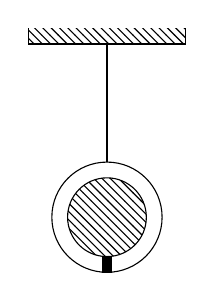
\begin{tikzpicture}
   \draw [pattern=north west lines] (-1,0.2)--(-1,0)--(1,0)--(1,0.2); 
   \draw (0,0)--(0,-1.5);
   \draw (0,-2.2) circle [radius=0.7];
   \draw [pattern=north west lines] (0,-2.2) circle [radius=0.5];
   \filldraw [color=black] (-0.06,-2.9) rectangle (0.06,-2.7);
 \end{tikzpicture}
 :>所示,一个空心均匀球壳里面注满水,球的正下方有一个小孔,在水由小孔慢慢流出的过程中,空心球壳和水的共同重心将会
 A.一直下降
 B.一直上升
 C.先升高后降低
 D.先降低后升高

 a.D

 e.当球壳中水满的情况时,重心在球心处,但是当水慢慢流出时,重心由对称性可知将会下降,但是当水流完之后,球壳的质量分布将再次均匀,所以重心还是在球心处,所以重心的变化必定是先降低再升高.

\end{selection}


  \newpage
  \section{弹力}
\subsection{弹性形变}
物体在力的作用下发生的形状或体积改变叫做形变.物体在受力后会发生形变,若撤去外力作用后,该物体能够恢复原状,则这种形变叫弹性形变.

\subsection{塑性形变}
物体受外力作用而使物体各部分相对位置的改变,当外力撤消后,物体不能恢复原状则这种形变称为塑性形变.

物体在受到足够大的外力作用时,会发生永久性的形状改变,这种在外力撤去后物体形状的改变可保存下来的性能叫做范性.现在更多的时候称作塑性.

\subsection{弹力的定义}
发生弹性形变的物体,由于要恢复原状,要对跟它接触的物体产生力的作用,这种作用叫做弹力.换种说法,也就是在弹性限度内,物体对使物体发生形变的施力物体产生的力叫做弹力.

\subsection{产生条件}

弹力是接触力,只能存在于物体相互接触处,但是相互接触的物体之间,并不一定有弹力的作用,因为接触不代表有形变.

产生弹力的条件:一,接触;二,有弹性形变.

注意:物体发生的弹性形变,不一定都能看出来,这称之为微小形变.任何物体中只要发生形变,就一定会对与它接触的物体产生弹力.一旦超出了弹性形变的限度就会完全失去弹力,这种超过了其弹性承受范围的形变称为``范性形变''.(即超过了弹性限度,塑性物体除外)

\subsection{弹力的方向}
受力物体所受弹力的方向与施力物体弹性形变的方向相反.具体可以有下列情况
\subsubsection{轻绳}
轻绳上的弹力方向沿绳指向绳收缩的方向.
\subsubsection{压力和支持力}
压力、支持力的方向总跟接触面垂直,面与面接触,点与面接触的情况,弹力都垂直于面;点与点的接触要找到公切面,弹力垂直于这个公切面指向被支持物.
\subsubsection{杆}
杆上的弹力可以指向任意方向, 在一个具体问题中,可以由它所受外力和运动状态决定.
\subsubsection{铰链}
一个杆如果一端使用一个轴固定住,但是可以自由转动,这个结构叫做铰链.这种情况杆上的力一定是沿着杆向里或者沿着杆向外.因为如果不沿杆,则这个杆会发生转动,所以可以判断一定是沿杆方向的.

\subsection{弹力的大小}
弹力的大小跟形变的大小的关系.在弹性限度内,形变越大,弹力也越大;形变消失,弹力就随着消失.对于拉伸形变(或压缩形变)来说,伸长(或缩短)的长度越大,产生的弹力就越大.对于弯曲形变来说,弯曲的越厉害,产生的弹力就越大.对于扭转形变来说扭转的越厉害,产生的弹力就越大.

\subsection{弹力的本质}
 弹力的本质是分子间的作用力.当物体被拉伸或者压缩时,分子间的距离便会发生变化,使分子间的相对位置拉开或者靠拢,这样,分子间的引力与斥力就不会平衡,出现相吸或者相斥的倾向,而这些分子间的吸引或者排斥的总效果,就是宏观上观察到的弹力.如果外力太大,分子间的距离被拉开得太多,分子就会滑进另一个稳定的位置,即使外力除去后,也不能回复到原位,就会保留永久的变形.这就是弹力的本质.

 \subsection{弹力的区别}
 弹力是按照力的性质命名的.而压力,支持力,拉力则是由力的效果命名的.这是两个完全不同的概念.因此,弹力和压力,支持力,拉力之间没有明确的关系.弹力不一定是压力,支持力,拉力.

 例如,套在同一光滑竖直杆的两个环形磁铁,其相同的磁极相对,两个磁铁均处于静止状态.对其中一个磁铁进行受力分析,磁铁受本身的竖直向下的重力作用和竖直向上的排斥力作用,二力为一对平衡力.此时,向上的排斥力便作为支持力.此支持力就不是弹力 .另外,由牛顿第三定律可以得到,大小等于向上的排斥力,方向向下的磁力也作用于下面的磁铁上.此时,这个向下的磁力就是上面的磁铁给它的向下的压力.这个压力也不是弹力.

 又如,在两根光滑平行直导轨间,分布有竖直方向且等间距分布的方向不同的匀强磁场,导轨上有一个宽度与磁场相同的金属框.当磁场匀速运动时,线框就会受到安培力作用而运动起来.此时,安培力就是线框运动的合外力,也就是拉力,但此拉力也不是弹力.

 注意:在这里出现的牛顿第三定律和安培力,在以后会讲到,此处主要为了说明弹力和压力,支持力,拉力之间的区别.基于以上讨论,不能笼统的说,弹力就是压力,支持力,拉力,要具体问题具体分析.
 
 \subsection{胡克定律}
 在\CJKunderwave{弹性限度内},弹簧弹力的大小$F$ 跟弹簧伸长(或缩短)的长度$x$成\CJKunderwave{正比}.即
 \begin{equation}
   F=kx
   \label{eq:hook law a}
 \end{equation}

k:弹簧的劲度系数,反映弹簧本身的属性,由弹簧自身的长度,粗细,材料等因素决定,与弹力$F$ 的大小和形变量$x$ 无关.

x:弹簧的形变量.记弹簧原长为$l_0$ ,发生形变后的长度为$l$,则弹簧的形变量为$x=|l-l_0|$

注意:此处的定义按人教版教材给出,只用式\eqref{eq:hook law a} 来计算弹力的大小,而方向则根据具体情况单独判断.

含方向的胡克定律:设弹簧伸长的方向为正,则$x=l-l_0$ ,于是可得
\begin{equation}
  F=-kx
  \label{eq:hook law b}
\end{equation}

在式\eqref{eq:hook law b} 中,如果弹簧伸长,则$l>l_0$ ,弹力与形变的方向相反,于是$F<0$ ,如果弹簧压缩$l<l_0$ ,则 $F>0$.

\subsection{例题分析}
 \begin{selection}
  1.下列关于弹力的几种说法,正确的是
  A.只要两物体接触就一定产生弹力
  B.静止在水平地面上的物体所受重力就是它对水平面的压力
  C.静止在水平面上的物体受到向上的弹力是因为地面发生了形变
  D.只要物体发生形变就一定有弹力产生

  a.C

  e.两物体接触并发生弹性形变才会产生弹力,A,D错误.静止在水平面上的物体所受重力的施力物体是地球,而压力的施力物体是该物体,受力物体是水平面,两力不同,B错误,C正确.

  2.两个光滑的木板固定为如<:
  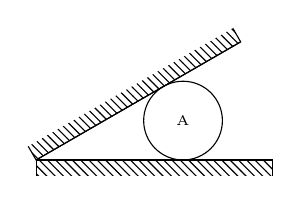
\begin{tikzpicture}
    \draw (0,0)--(3,0);
    \draw (1.866,0.5) node {\tiny A} circle [radius=0.5cm];
    \draw [rotate=30] (0,0)--(3,0);
    \draw [pattern=north west lines] (0,-0.2)--(0,0)--(3,0)--(3,-0.2);
    \draw [rotate=30,pattern=north west lines] (0,0.2)--(0,0)--(3,0)--(3,0.2);
  \end{tikzpicture}
  :>的结构,其中下面的木板水平,小球$A$ 放于其中且与两木板都接触,则
  A.两个木板对$A$ 都有弹力作用
  B.只有下面的木板对$A$ 有弹力作用
  C.将图中结构整体逆时针旋转一小角度后,$A$ 球受两木板的弹力作用
  D.将图中结构整体逆时针旋转一小角度后,球$A$ 仅受左边木板的弹力作用

  a.BC

  e.接触但是如果没有形变则不会有弹力.一般的微小形变没法直接看出来,则采用假设法.假设撤去上面的木板,则$A$ 仍会静止不动,但撤去下面的木板,$A$ 会掉下来,故$B$ 正确,同理可得C正确.

  3.在半球形光滑碗内,斜搁一根筷子,如<:
  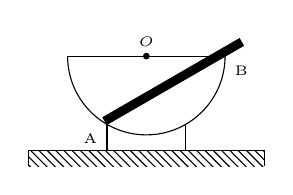
\begin{tikzpicture}
    \draw (-1,0) arc (180:360:1); 
    \draw (-1,0)--(1,0)node [anchor=north west]{\tiny B};
    \filldraw (0,0) node [anchor=south]{\tiny $O$} circle [radius=1pt];
    \filldraw [black,rotate around={30:(-0.5,-0.866)}] (-0.5,-0.866) rectangle (1.5,-0.766) ;
    \draw (-0.5,-0.866) node [anchor=north east]{\tiny A}--(-0.5,-1.2);
    \draw (0.5,-0.866) --(0.5,-1.2);
    \draw [pattern=north west lines] (-1.5,-1.4)--(-1.5,-1.2)--(1.5,-1.2)--(1.5,-1.4);
  \end{tikzpicture}
  :>所示,筷子与碗的接触点分别为$A$ ,$B$,则碗对筷子$A$ , $B$ 两点处的作用力方向分别为
  A.均竖直向上
  B.均指向球心$O$
  C.$A$ 点处指向球心$O$ ,$B$ 点处竖直向上
  D.$A$点处指向球心$O$,$B$ 处垂直于筷子斜向上

  a.D

  e.碗对筷子$A$ ,$B$ 两点处的作用力属于弹力,而接触处的弹力总是垂直于接触面,因而寻找接触面便成为确定弹力方向的关键.在$A$ 点处,当筷子滑动时,筷子与碗的接触点在碗的内表面(半球面)上滑动,所以在$A$ 点处的接触面是球面在该点的切面,此处弹力与切面垂直,即指向球心$O$.在B点处,当筷子滑动时,筷子与碗的接触点在筷子的下表面上滑动,所以在$B$点处的接触面与筷子平行,此处的弹力垂直于筷子斜向上.

 \end{selection}
 \begin{calculate}
   4.一根轻质弹簧,当它受到$10N$ 的拉力时长度为$12cm$, 当它受到$25N$ 的拉力时长度为$15cm$.问:(注意:弹簧始终在弹性限度内)
   [1]弹簧不受力时的自然长度为多长?
   [2]该弹簧的劲度系数为多大?

   a. $0.1m $ \qquad $500N/m$

   e.设弹簧的劲度系数为$k$,原长$l_0$ ,由\eqref{eq:hook law a}式得
   $$F_1=k(l_1-l_0)$$
   $$F_2=k(l_2-l_0)$$
   (1)以第一式除以第二式,消去$k$得
   $$\cfrac{F_1}{F_2}=\cfrac{l_1-l_0}{l_2-l_0}$$
   解得
   $$l_0=\cfrac{F_1l_2-F_2l_1}{F_1-F_2}=0.1m$$
   (2)以上述第一式减去第二式,消去$l_0$得
   $$k=\cfrac{F_1-F_2}{l_1-l_2}=500N/m$$



 \end{calculate}

  \newpage
  \section{摩擦力}
\subsection{定义}
阻碍物体\CJKunderwave{相对运动}(或者\CJKunderwave{相对运动趋势})的力叫做摩擦力.
\subsection{方向}
摩擦力存在于相互接触的两个物体间,则\CJKunderwave{受力物体所受摩擦力}的方向与\CJKunderwave{受力物体相对于施力物体的运动(或相对运动趋势)}的方向相反.

同学们注意,相对运动这点比较容易看出来,但是相对运动的趋势则用肉眼不能看出来,解决的方法是\CJKunderwave{假设法},即:假设没有摩擦则看物体将向哪个方向运动,则此运动方向就是相对运动趋势的方向.相对运动的趋势本质上是微观上原子之间相对位置发生了变化,但是没有宏观上的运动.

\subsection{摩擦力的分类}
\subsubsection{静摩擦力}
两个相互接触的物体,当其接触表面之间有相对运动的趋势,但尚保持相对静止时,彼此作用着阻碍相对滑动的阻力,这种阻力称为静滑动摩擦力,简称为静摩擦力.静摩擦力产生的条件为:
\begin{enumerate}
  \item 相互接触,且接触面粗糙
  \item 有弹力(或者形变)
  \item 有相对运动的趋势
\end{enumerate}

静摩擦力的大小是一个范围,它会根据外界的受力情况而自动作出调整.当外力超过一定的限度时,物体和物体之间将会发生相对滑动,能够保持物体之间相对静止的最大的静摩擦力叫做最大静摩擦力,用符号$f_{max}$  表示.用公式表达就是
\begin{equation}
  0\leqslant f\leqslant f_{max}
  \label{eq:jingmoca}
\end{equation}

\subsubsection{滑动摩擦力}
当一物体在另一物体表面上滑动时,在两物体接触面上产生的阻碍它们之间相对滑动的力叫做滑动摩擦力.滑动摩擦力产生的条件为:
\begin{enumerate}
  \item 相互接触,且接触面粗糙
  \item 有弹力(或者形变)
  \item 有相对运动
\end{enumerate}

滑动摩擦力的大小,由库仑摩擦定律来确定,即下式
\begin{equation}
  f=\mu F_N
  \label{eq:dongmoca}
\end{equation}

在\eqref{eq:dongmoca} 式中,$\mu$叫做动摩擦因数,取决于相互接触的两个物体在粗糙程度和材料等因素.$F_N$ 是二物体接触面的正压力,$f$ 是滑动摩擦力.由\eqref{eq:dongmoca}式容易得到\CJKunderwave{滑动摩擦力与接触面积无关}.

\subsubsection{滚动摩擦力}
一物体在另一物体表面做无滑动的滚动或有滚动的趋势时,由于物体在接触部分受压发生形变而产生的对滚动的阻碍作用,叫滚动摩擦.它的实质是静摩擦力.由于在高中阶段暂未涉及滚动摩擦力,这里提出来仅作为知识上的完备,不作深入讨论.

\subsection{例题分析}

\begin{selection}
1.如<:
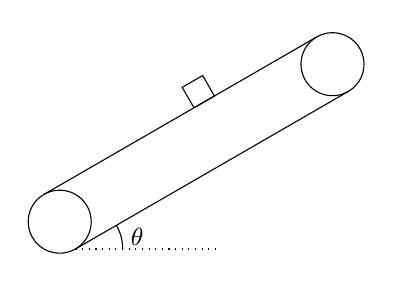
\begin{tikzpicture}
  \draw [dotted] (0.2,0.053589838)--(2,0.053589838); 
  \draw (0,0.4) circle [radius=0.4cm] ;
  \draw[rotate around={30:(0,0.4)}] (4,0.4) circle [radius=0.4cm] ;
  \draw[rotate around={30:(0.2,0.053589838)}] (0.2,0.053589838)--(4.2,0.053589838); 
  \draw[rotate around={30:(-0.2,0.7464)}] (-0.2,0.7464)--(3.8,0.7464); 
  \draw[rotate around={30:(-0.2,0.7464)}] (2,0.7464) rectangle (2.3,1.0464); 
  \draw (0.8,0.053589838) arc (0:30:0.6);
  \draw [rotate around={15:(0.2,0.053589838)}] (0.8,0.053589838) node [anchor=west]{\small $\theta$};
\end{tikzpicture}
:>所示,为倾斜的皮带传送装置.关于传送带上的物体所受的摩擦力,下列说法正确的是
A.若传送带静止,物体也静止,则物体受到沿传送带向上的摩擦力
B.若传送带静止,物体也静止,则物体受到沿传送带向下的摩擦力
C.若传送带顺时针匀速转动,物体随传送带一起向做匀速运动,则物体受到沿传送带向上的静摩擦力
D.若传送带顺时针匀速转动,物体随传送带一起向做匀速运动,则物体受到沿传送带向上的滑动摩擦力
  
a.AC

e.物体静止在静止的传送带上时,或物体随传送带一起向上匀速运动的过程中,都具沿传送带下滑的趋势,这个趋可以假设传送带光滑然后物体一定在重力作用下向下滑动判断出来,所以物体均受到沿传送带向上的静摩擦力作用.

\end{selection}

\begin{calculate}
  2.如<:
  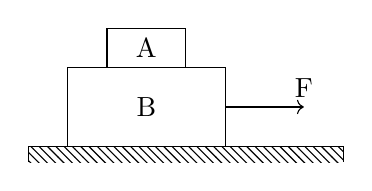
\begin{tikzpicture}
   \draw (-1,0) rectangle (1,1); 
   \draw (0,0.5) node {B};
   \draw (-0.5,1) rectangle (0.5,1.5);
   \draw (0,1.25) node {A};
   \draw [->](1,0.5) -- (2,0.5) node [anchor = south] {F};
   \draw [pattern=north west lines] (-1.5,-0.2)--(-1.5,0)--(2.5,0)--(2.5,-0.2);
  \end{tikzpicture}
  :>所示,物体$A$ ,$B$ 在外力作用下共同做匀速运动,$A$ 是否受到摩擦力?

  a.不受摩擦力

  e.$A$ 物体保持静止,所以受力是平衡的,假设$A$ 受到摩擦力,但是在水平方向找不到一个力与此力平衡的力,所以假设错误,因此$A$ 不受摩擦力.

  3.质量为$2kg$ 的物体静止在水平地面上,如<:
  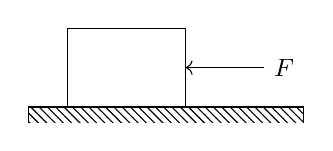
\begin{tikzpicture}
    \draw (0,0) rectangle (1.5,1);
    \draw [->] (2.5,0.5) node [anchor=west]{\small $F$} -- (1.5,0.5);
   \draw [pattern=north west lines] (-0.5,-0.2)--(-0.5,0)--(3,0)--(3,-0.2);
  \end{tikzpicture}
  :>所示,物体与地面间的动摩擦因数为$0.5$ ,最大静摩擦力与滑动摩擦力视为相等,给物体一水平推力$F$.(取$g=10m/s^2$)

  a.(1) $5N$ \qquad (2) $10N$ \qquad (3) $10N$

  e.在地面上,由竖直方向受力平衡得$F_N=mg$ ,则滑动摩擦力由\eqref{eq:dongmoca} 式得
  $$f=\mu F_N=0.5\times 2\times 10N=10N$$
  题中认为最大静摩擦力等于滑动摩擦力,所以$f_{max}=10N$
  \newline
  (1)当推力$F=5N$ 时,$F<f_{max}$ ,则物体保持静止,由二力平衡知,地面对物体的静摩擦力大小为
  $$F_{\mbox{\tiny 静}}=F=5N$$
  (2)当推力$F=12N$时,$F>f_{max}$,物体滑动.则地面对物体的滑动摩擦力大小为
  $$F_{\mbox{\tiny 滑}}=\mu F_N=\mu mg=10N$$
  (3)物体运动过程中突然把推力去掉,地面对物体的摩擦力为滑动摩擦力,其大小同(2)中计算得
  $$F_{\mbox{\tiny 滑}}=\mu F_N=\mu mg=10N$$

\end{calculate}

  \newpage
  \section{力的合成}
\subsection{基本规则}

力是矢量,所有的矢量都必须遵守平行四边行定则(或三角形定则).为清析起见,重绘图\ref{fig:parallelogram law}在此处,但是将符号改为对应的力的符号:合力$F$,分力$F_1$和$F_2$,两个分力之间的夹角为$\theta$.

\begin{figure}[H]
  \centering
  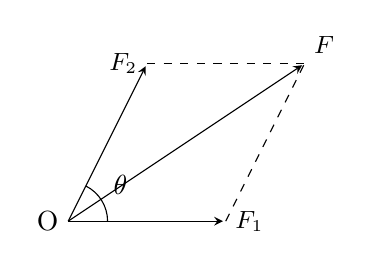
\begin{tikzpicture}
    \draw [->,>=stealth,shorten >=1pt] (0,0)--(2,0) node [anchor=west]{\small $F_1$};
    \draw [->,>=stealth,shorten >=1pt] (0,0)--(1,2) node [anchor=east]{\small $F_2$};
    \draw [dashed] (1,2) --(3,2);
    \draw [dashed] (2,0)--(3,2);
    \draw [->,>=stealth,shorten >=1pt] (0,0)--(3,2) node [anchor=south west]{\small $F$};
    \draw (0,0) node [anchor=east]{O};
    \draw (0.5,0) arc (0:63.43495:0.5);
    \draw (25:0.5) node [anchor=south west]{$\theta$};
  \end{tikzpicture}
  \caption{力的合成}
\end{figure}

由余弦定理容易得到合力与分力的数量关系如下:
\begin{equation}
  F=\sqrt{F_1^2+F_2^2+2F_1F_2\cos\theta}
  \label{eq:cosine law}
\end{equation}

由于夹角范围 $0\leqslant \theta \leqslant \pi$ ,所以$\cos\theta$ 是单调递减的,因此随两个分力的夹角的增大,合力的大小逐渐减小.当$\theta=0$ 时,合力最小,当$\theta=\pi$ 时,合力最大,即
\begin{equation}
  |F_1-F_2|\leqslant F \leqslant F_1+F_2
  \label{eq:resultant force}
\end{equation}

如果知道了两个分力作为矢量的坐标,也可以使用矢量的坐标运算解决.记$F_1=(x_1,y_1)$,$F_2=(x_2,y_2)$,则合力可以表达为
\begin{equation}
  F=\sqrt{(x_1+x_2)^2+(y_1+y_2)^2}
  \label{eq:coordinate force}
\end{equation}
\subsection{余弦定理的证明}
如果同学们是初学者,则按现行的高中数学教材,还没有学到余弦定理,但是此定理无论在数学还是物理上都是十分重要的,所以这里为同学们加以证明.

首先由勾股定理证明一个结论:$\cos^2\theta+\sin^2\theta=1$.如下图
\begin{figure}[H]
  \centering
  \begin{tikzpicture}
    \draw (0,0) node [anchor=east]{A}--(4,0) node [anchor=west]{B}--(4,3) node [anchor=west]{C}--(0,0)--cycle; 
    \draw (0.8,0) arc (0:37:0.8);
    \draw (18.5:0.8) node [anchor=west] {$\theta$};
  \end{tikzpicture}
  \caption{勾股定理}
  \label{fig:gougu law}
\end{figure}

记边长$BC=a$,$AC=b$,$AB=c$,则由勾股定理得
$$a^2+b^2=c^2$$
对上式,左右同时除以$c^2$,得
$$\Big (\cfrac{a}{c} \Big )^2+\Big (\cfrac{b}{c} \Big )^2=1$$
根据三角函数定义$\sin \theta=\frac{a}{c}$ 和 $\cos\theta=\frac{b}{c}$ 上式可以用三角函数表达为
\begin{equation}
\cos^2\theta+\sin^2\theta=1
  \label{eq:gougu}
\end{equation}

如图\ref{fig:cosine law}所示,记边长$BC=a$,$AC=b$,$AB=c$
\begin{figure}[H]
  \centering
  \begin{tikzpicture}
    \draw (0,0) node [anchor=east]{A}--(1.5,0) node [anchor=north]{D}--(3.5,0) node [anchor=west]{B} -- (1.5,2) node [anchor=south] {C} -- (0,0)--cycle; 
    \draw (1.5,0)--(1.5,2);
    \draw (0.3,0) arc (0:53:0.3);
    \draw (15:0.3) node [anchor= south west] {$\theta$};
    \draw (1.75,-0.3) node [anchor=north] {\small 甲};
  \end{tikzpicture}
  \qquad
  \begin{tikzpicture}
    \draw (0,0) node [anchor=east] {D}--(1.5,0) node [anchor=north]{A}--(4,0) node [anchor=west]{B} -- (0,2) node [anchor=south] {C}--(0,0) -- cycle; 
    \draw (0,2)--(1.5,0);
    \draw (1.8,0) arc (0:127:0.3);
    \draw (1.634,0.268) node [anchor=south west] {$\theta$};
    \draw (2,-0.3) node [anchor=north] {\small 乙};
  \end{tikzpicture}
  \caption{余弦定理}
  \label{fig:cosine law}
\end{figure}

在图\ref{fig:cosine law} 甲所示,由三角函数定义易得$CD=b\sin\theta$,$AD=b\cos\theta$,所以$BD=c-b\cos\theta$,由勾股定理得
$$(b\sin\theta)^2+(c-b\cos\theta)^2=a^2$$
将上式展开得
$$b^2(\cos^2\theta+\sin^2\theta)+c^2-2bc\cos\theta=a^2$$
代入\eqref{eq:gougu}式得
$$b^2+c^2-2bc\cos\theta=a^2$$
对于图\ref{fig:cosine law} 乙所示,当$\theta >90^\circ$ 时,定义正弦函数 $\sin\theta=\sin(\pi-\theta)$,余弦函数$\cos\theta=-\cos(\pi -\theta)$.显然式\eqref{eq:gougu} 仍然满足.由三角函数定义可得$AD=b\cos(\pi -\theta)=-b\cos\theta$,$CD=b\sin(\pi-\theta)=b\sin\theta$,由勾股定理得
$$(c-b\cos\theta)^2+(b\sin\theta)^2=a^2$$
经过简单运算同样得
$$b^2+c^2-2bc\cos\theta=a^2$$
上式就是余弦定理.

\eqref{eq:cosine law}式,可以由余弦定理得到,如下
$$F_1^2+F_2^2-2F_1F_2\cos(\pi-\theta)=F^2$$
代入$\cos(\pi-\theta)=-\cos\theta$,同时再开方,移项得
$$F=\sqrt{F_1^2+F_2^2+2F_1F_2\cos\theta}$$


\subsection{正弦定理的证明}

在物体的受力平衡问题中,特别是三力平衡问题中,三个力构成封闭矢量三角形.这类问题的求解和讨论更多的是归结为解三角形,讨论三角形三个边和角的关系.所以正弦定理就相当必要在这里阐述.

\subsubsection{正弦定理}
如图\ref{fig:zhengxian}所示,记三角形的三个角分别为:A,B和C;对应的三条边分别记为:a,b和c.则有关系
\begin{equation}
  \frac{a}{\sin A}=\frac{b}{\sin B}=\frac{c}{\sin C}
  \label{eq:zhengxian}
\end{equation}

\begin{figure}[H]
  \centering
  \begin{tikzpicture}
    \draw (0,0) node [anchor=east]{\small A}--++(30:4) node [anchor=west]{\small B}--++(-45:3) node [anchor=south]{\small C}--(0,0)--cycle;
    \draw (30:0.4) arc (30:0:0.4);
    \draw (0,0)++(30:3.6) arc (210:315:0.4);
    \draw (0,0)++(30:4)++(-45:2.6) arc (135:180:0.4);
    \draw (32:2) node [anchor=east]{\small c};
    \draw (30:4)++(-42:1.5) node [anchor=west]{\small a};
    \draw (3,0) node [anchor=north]{\small b};
  \end{tikzpicture}
  \caption{正弦定理}
  \label{fig:zhengxian}
\end{figure}

\subsubsection{正弦定理的证明}

如图\ref{fig:zhengxian1}所示,任何一个三解开必有一个外接圆,由平面几何易知,圆周角是圆心角的一半,在图\ref{fig:zhengxian1}中$OD$垂直于$BC$,由于$OB=OC$所以$OD$又是$\angle BOC$的平分线,则$\angle BOD=A$,由几何关系可得三解形外接圆的半径为

\[
  R=\frac{a}{2\sin A}
\]

同理由其它二个角也可以写出半径
\[
  R=\frac{b}{2\sin B}=\frac{c}{2\sin C}
\]

将三个求半径的式子写到一块,同时乘以$2$化成直径,则得到正弦定理

\[
  2R=\frac{a}{\sin A}=\frac{b}{\sin B}=\frac{c}{\sin C}
\]


\begin{figure}[H]
  \centering
  \begin{tikzpicture}
    \draw (0,0) circle [radius=2];
    \draw [dashed] (0,0)--(53:2) node [anchor=west]{\small A};
    \draw [dashed] (0,0)--(-60:2) node [anchor=west]{\small C};
    \draw [dashed] (0,0)--(180:2) node [anchor=east]{\small B};
    \draw (53:2)--(180:2)--(-60:2)--(53:2)--cycle;
    \draw[dashed] (0,0)--(-120:1) node [anchor=east]{\small D};
    \filldraw (0,0) circle [radius=1pt] node [anchor=south east]{\small O};
    \draw (180:0.4) arc (180:240:0.4);
    \draw (210:0.5) node {\small A};
  \end{tikzpicture}
  \caption{正弦定理证明}
  \label{fig:zhengxian1}
\end{figure}
\subsection{注意事项}
力是矢量,遵守平行四边行定则 ,但是在考虑实际问题时并不是所有的情况都可以使用力的合成.能够进行力的合成的情况,只能是所谓的共点力.

共点力:如果几个力共同作用在\CJKunderwave{同一点} 上,或者虽不作用在同一点上,但是它们的\CJKunderwave{作用线}交于一点,这样的一组力叫做共点力.

  \newpage
  \section{力的分解}
\subsection{基本原理}
力是矢量,力的加减满足平行四边形定则.力的合成的逆运算叫做力的分解.也就是\CJKunderwave{已知一个力求它的分力}的过程.

在这里有必要解释一下,研究力的分解的深刻含义:举一个例子,在小学大家刚开始学习算术的时候,老师教大家计算$13+27=?$,这可以先拆开再相加,则运算简洁快速不少,如下
$$13+27=10+3+20+7=10+20+(3+7)=40$$

力是一个矢量,则多个矢量相加,按平行四边形定则可行,但是具体运算要复杂的多,因为要画多个平行四边形,同时每个平行四边形都要使用余弦定理计算,涉及开方和三角函数运算.为了方便运算,往往需要采用先分解为两个相互垂直的方向的分力,然后再把每个坐标轴上的分力叠加起来,最后再使用勾股定理计算则可以简化许多---这个方法叫做正交分解法.

力的分解与力的合成不同,力的合成结果是唯一的,但是力的分解,是将一个力分解为二个力或多个力,这在数学上有无数种分解方式,就象$9=1+8=2+7=\cdots $一样.正是力的分解的这种任意性,结合实际情况可以将计算变的大为简化.根据实际情况,可以定出如下力的分解法:
\begin{enumerate}
  \item 根据\CJKunderwave{力的实际作用}效果定出两个分力的方向
  \item 根据\CJKunderwave{两个分力}的方向作出平行四边形
  \item 利用数学知识\CJKunderwave{解三角形},分析,计算分力的大小.
\end{enumerate}
\subsection{例题分析}
\begin{calculate}
 1.如<:
 \begin{tikzpicture}
   \draw (-0.2,1.5) rectangle (-1pt,-1.5);
   \draw (0,0) circle [radius=1pt];
   \draw (-1pt,-1pt) rectangle (2.598,1pt) node [anchor=west]{\small $O$};
   \draw (-1pt,1.5) -- (2.598,1pt);
   \draw (2.598,1pt)--(2.598,-1);
   \draw (2.398,-1) rectangle (2.798,-1.4);
   \draw (2.165,0.254) arc (150:177:0.5);
   \draw (2.098,0) node [anchor=south east]{\small $30^\circ$};
 \end{tikzpicture}
 :>所示,轻杆与柱子之间用铰链连接,杆的末端吊着一个重为$30N$ 的物体,轻绳与水平轻杆之间的夹角为$\theta=30^\circ$ ,求轻绳和杆各受到多大的力?(结果保留两位有效数字)

 a.$60N$ \qquad $52N$

 e.物体静止则受力平衡,所以重力与竖直绳的拉力平衡,则竖直绳的拉力大小$F=G$.由于绳的拉力一定沿绳指向绳收缩的方向,铰链所受力的方向一定沿杆的方向.所以得出力分解的两个效果的方向就是绳收缩的方向和杆压缩的方向.由此作平行四边形如
 <:
 \begin{tikzpicture}
   \draw (-0.2,1.5) rectangle (-1pt,-1.5);
   \draw (0,0) circle [radius=1pt];
   \draw (-1pt,-1pt) rectangle (2.598,1pt) node [anchor=west]{\small $O$};
   \draw (-1pt,1.5) -- (2.598,1pt);
   \draw (2.598,1pt)--(2.598,-1);
   \draw (2.398,-1) rectangle (2.798,-1.4);
   \draw (2.165,0.254) arc (150:177:0.5);
   \draw (2.098,0) node [anchor=south east]{\small $30^\circ$};
   \draw [->](2.589,0)--(0,0) node [anchor=south]{\small $F_2$};
   \draw [->](2.589,0)--(2.589,-1.4948) node [anchor=east] {\small $F=G$};
   \draw [->](2.589,0)--(5.178,-1.4948) node [anchor=west] {\small $F_1$};
   \draw [dashed] (0,0)--(2.589,-1.4948);
   \draw [dashed] (5.178,-1.4948)--(2.589,-1.4989);
 \end{tikzpicture}
 :>所示,由几何关系得
 $$F_1=\cfrac{G}{\sin\theta}=60N,F_2=\cfrac{G}{\tan\theta}\approx 52N$$

 \end{calculate}

 \newpage

 \begin{selection}
 2.如<:
 \begin{tikzpicture}
   \draw (0,0) node [anchor=east] {\small O}--(3,0) node [anchor=north east] {\small $F_2$ 的方向};
   \draw [->,>=stealth] (0,0)--(2,1.5) node [anchor=east] {$F$};
   \draw (0.3,0) arc (0:37:0.3);
   \draw (30:0.3) node [anchor=west]{\small $\theta$};
 \end{tikzpicture}
 :>所示,将力$F$ (大小已知)分解为两个分力$F_1$ 和$F_2$ ,$F_2$ 和$F$ 的夹角$\theta$ 小于 $90^\circ$ ,则下列说法正确的是
 A.当$F_1>\sin\theta$ 时,肯定有两组解
 B.当 $F>F_1>F\sin\theta$ 时,肯定有两组解
 C.当$F_1<F\sin\theta$ 时,有唯一一组解
 D.当$F_1<F\sin\theta $ 时,无解.

 a.BD

 e.已知合力的大小、一个分力的方向,根据平行四边形定则(三角形定则更方便)作图,如
 <:
 \begin{tikzpicture}
   \draw (0,0) node [anchor=east] {\small O}--(5,0) node [anchor=north east] {\small $F_2$ 的方向};
   \draw [->,>=stealth] (0,0)--(2,1.5) node [anchor=east] {\small $F$};
   \draw (0.3,0) arc (0:37:0.3);
   \draw (30:0.3) node [anchor=west]{\small $\theta$};
   \draw  (2,0)--(2,1.5) node [anchor=west] {\small $F_1$};
   \draw  (1,0)--(2,1.5) node [anchor=west] {\small $F_1$};
   \draw  (2.5,0)--(2,1.5) node [anchor=west] {\small $F_1$};
   \draw  (4.5,0)--(2,1.5) node [anchor=west] {\small $F_1$};
   \draw (2,0) rectangle (2.2,0.2);
 \end{tikzpicture}
 :>所示
 \newline
 当$F>F_1>F\sin\theta$ , 一定有两组解
 \newline
 当 $F_1>F$ 时,有唯一一组解
 \newline
 当$F_1<F\sin\theta $ ,无解.
 
 \end{selection}

 \begin{calculate}
3.如<:
\begin{tikzpicture}
  \draw (0,0) rectangle (1,0.8);
  \draw [dashed] (0.5,0.4)--(1.5,0.4);
  \draw[->,>=stealth] (0.5,0.4) -- (1.5,0.97735) node [anchor=west] {\small $F$};
  \draw[pattern=north west lines] (-0.5,-0.2)--(-0.5,0)--(1.5,0)--(1.5,-0.2);
  \draw (0.8,0.4) arc (0:30:0.3);
  \draw (0.7,0.3) node [anchor=south west] {\tiny $\theta$};
\end{tikzpicture}
:>所示,水平面上有一重$60N$的物体,在与水平方向成$30^\circ$ 角斜向上,大小为$20N$的拉力作用下匀速运动,求地面对物体的支持力和摩擦力的大小.

a.$50N$ \quad $10\sqrt{3}N$

e.对物体进行受力分析,如<:
\begin{tikzpicture}
  \draw (0,0) rectangle (1,0.8);
  \draw [dashed] (0.5,0.4)--(1.5,0.4);
  \draw[->,>=stealth] (0.5,0.4) -- (1.5,0.97735) node [anchor=west] {\small $F$};
  \draw[pattern=north west lines] (-0.5,-0.2)--(-0.5,0)--(1.5,0)--(1.5,-0.2);
  \draw (0.8,0.4) arc (0:30:0.3);
  \draw (0.7,0.3) node [anchor=south west] {\tiny $\theta$};
  \draw [->,>=stealth] (-1,0.4)--(2,0.4) node [anchor=north]{\small $x$};
  \draw [->,>=stealth] (0.5,-1)--(0.5,2) node [anchor=west] {\small $y$};
  \draw [dashed](1.5,0.4)--(1.5,0.97735);
  \draw [->,>=stealth] (0.5,0.4)--(1.5,0.4) node [anchor=north] {\tiny $F_x$};
  \draw [dashed](0.5,0.97735) --(1.5,0.97735);
  \draw [->,>=stealth] (0.5,0.4)--(0.5,0.97735) node [anchor=east]{\tiny $F_y$};
  \draw [->,>=stealth] (0.5,0.4)--(0.5,1.5) node [anchor=east] {\tiny $F_N$};
  \draw [->,>=stealth] (0.5,0.4)--(-0.5,0.4) node [anchor=north] {\tiny $F_f$};
\end{tikzpicture}
:>所示,物体受重力$G$,支持力$F_N$,拉力$F$,摩擦力$F_f$.建立正交直角坐标系,对力$F$ 进行正交分解得两个分力的大小分别为
$$F_x=F\cos\theta,F_y=F\sin\theta$$
$y$方向受力平衡:
$$F_N+F\sin30^\circ -G=0$$
$x$方向受力平衡:
$$F_f-F\cos30^\circ =0$$
以上两式联立解得:
$$F_N=50N,F_f=10\sqrt{3}N$$

ee.注意:在使用正交分解法时,坐标系的建立原则上是任意的,它都能解决问题.但是实际使用时,要兼顾计算的简洁,如果将坐标轴建立在相互垂直的力上,且使尽量多的力落在坐标轴上,那么需要分解的力就少了,这样就能减少计算量.比如这里,支持力$F_N$和摩擦力$F_f$相互垂直,则按这个规则建立坐标轴后,只有拉力$F$ 需要分解,这样计算量就减少了.同学们在使用时要仔细研究分析之后选择最简单的建立坐标系的才能不断提高解题能力.

\end{calculate}
\begin{selection}
4.如<:
\begin{tikzpicture}
  \draw (1,0) node [anchor= south west] {\tiny $D$} arc (0:180:1);
  \draw [pattern=north west lines] (-1.5,-0.2)--(-1.5,0)--(-0.5,0)--(-0.5,-0.2);
  \draw [pattern=north west lines] (1.5,-0.2)--(1.5,0)--(0.5,0)--(0.5,-0.2);
  \draw [dashed] (-1,0)--(1,0);
  \draw (0,0) node [anchor=north] {\tiny $O$}-- (135:1) node [anchor=south east] {\tiny $B$};
  \draw (0,0) --(45:1) node [anchor=south west] {\tiny $A$};
  \draw (0,0) -- (0,-1);
  \draw (-0.2,-1) rectangle (0.2,-1.4);
  \draw (0,-1.2) node {\tiny $M$};
  \draw [dashed] (0,0)--(0,1) node [anchor=south] {\tiny $C$};
\end{tikzpicture}
:>所示,质量为$M$ 的物体用$OA$ 和$OB$ 两根等长的绳子悬挂在半弧形的支架上,$B$ 点固定不动,$A$ 点则由顶点$C$ 沿圆弧向$D$ 移动.在此过程中,绳子$OA$ 的张力将
A.由大变小
B.由小变大
C.先减小再增大
D.先增大再减小

a.C

e.此题目画三角形更方便一些.如<:
\begin{tikzpicture}
  \draw (1,0) node [anchor= south west] {\tiny $D$} arc (0:180:1);
  \draw [pattern=north west lines] (-1.5,-0.2)--(-1.5,0)--(-0.5,0)--(-0.5,-0.2);
  \draw [pattern=north west lines] (1.5,-0.2)--(1.5,0)--(0.5,0)--(0.5,-0.2);
  \draw [dashed] (-1,0)--(1,0);
  \draw (0,0) node [anchor=north] {\tiny $O$}-- (135:1) node [anchor=south east] {\tiny $B$};
  \draw (0,0) --(45:1) node [anchor=south west] {\tiny $A$};
  \draw (0,0) -- (0,-1);
  \draw (-0.2,-1) rectangle (0.2,-1.4);
  \draw (0,-1.2) node {\tiny $M$};
  \draw [dashed] (0,0)--(0,1) node [anchor=south] {\tiny $C$};
  \draw [->,>=stealth] (0,0)--(0,-2) node [anchor=north east] {\tiny $Mg$};
  \draw [<-,>=stealth] (0,0) -- (315:2);
  \draw [->,>=stealth] (0,-2) -- +(45:1.414) node [anchor=south west]{\tiny 1};
  \draw [->,>=stealth] (0,-2)-- (0.7071,-0.7071) node [anchor=south west]{\tiny 2};
  \draw [->,>=stealth] (0,-2)-- (1.414,-1.414) node [anchor=south west]{\tiny 3};
  \draw (0,-0.3) arc (270:315:0.3);
  \draw (270:0.2) node [anchor=north west]{\tiny $\theta$};
\end{tikzpicture}
:>所示,画出了三种情况力的三角形,当$OA$ 的力在 1位置时,$F_A$ 与 $F_B$ 垂直,此时$F_A=Mg\sin\theta$ 是最小的.当 $OA$ 的力 在2或者 3位置时,$F_A>Mg\sin\theta$,所以绳子 $OA$ 的张力先减小再增大.
\newline
同学们注意:在力的动态变化分析时,一般会是三个力,已知一个力的大小和方向,第二个力的方向,问第三个力的情况.这时候画力的三角形要比平行四边形简单的多.如果物体的受力个数超过三个,则应当据正交分解法求出所讨论的力的大小与角度的关系,然后据函数的增减性来判断,会更加清析一些.

\end{selection}
\newpage
\begin{selection}
  
1.(多选)如<:
\begin{tikzpicture}
  \draw [pattern=north west lines] (-1.5,-0.2)--(-1.5,0)--(1.5,0)--(1.5,-0.2);
  \draw (-1,0) -- (1,0) -- (1,1.5) -- (-1,0)--cycle;
  \draw [rotate around={37:(-1,0)}] (0.4,0) rectangle (0.8,0.4);
  \draw [->,>=stealth,rotate around={37:(-1,0)}] (0.6,0.2) -- + (-127:1) node [anchor=west] {\small $mg$};
  \draw [->,>=stealth,rotate around={37:(-1,0)}] (0.6,0.2) -- + (-0.60182,0) node [anchor=east] {\small $F_1$};
  \draw [->,>=stealth,rotate around={37:(-1,0)}] (0.6,0.2) -- + (0,-0.79864) node [anchor=west] {\small $F_2$};
  \draw [dashed,rotate around={37:(-1,0)}] (-0.00182,-0.59864) -- (0.6,-0.59864);
  \draw [dashed,rotate around={37:(-1,0)}] (-0.00182,-0.59864) -- (-0.00182,0.2);
  \draw [->,>=stealth,rotate around={37:(-1,0)}] (0.6,0.2) -- (0.6,1) node [anchor=east] {\small $F_N$}; 
\end{tikzpicture}
:>所示,光滑斜面上物体重力$mg$ 分解为$F_1$ 和$F_2$ 两个力,下列说法正确的是
A.物体受到重力$mg$ , $F_N$ , $F_1$ ,$F_2$ 四个力作用
B.物体只受到重力$mg$ 和斜面的支持力$F_N$ 的作用
C.$F_1$ 是斜面作用在物体上使物体下滑的力,$F_2$ 是物体对斜面的压力
D.力$F_N$ ,$F_1$,$F_2$ 三力的作用效果与力$mg$ ,$F_N$ 两个力的作用效果相同

a.BD

e.由重力的作用效果分析,再由力产生的原因进行判断$F_1$ 和$F_2$ 两个力是重力$mg$ 的两个分力,其作用效果与重力$mg$ 等效,所以$F_2$ 不是物体对斜面的压力,物体只受重力$mg$ 和斜面的支持力$F_N$ 的作用,故 B,D正确.

\end{selection}
\begin{calculate}
  1. 如 
  <:
\begin{tikzpicture}
  \draw[pattern=north west lines] (-0.5,1.7)--(-0.5,1.5)--(0.5,1.5)--(0.5,1.7);
  \draw (0,0.2)--(0,1.5);
  \draw (0,0) circle [radius=2mm];
  \draw (0,-0.5) node [anchor=north] {\small 甲};
\end{tikzpicture}
  \qquad
\begin{tikzpicture}
  \draw (-1,0)--(-0.5,0);
  \draw (-0.5,0) arc (180:360:0.5);
  \filldraw[black] (0,0) node [anchor=south] {\small $O$} circle [radius=1pt];
  \draw (0.5,0)--(1,0);
  \draw[black,rotate around={26.5:(-0.3,-0.4)}] (-0.3,-0.4) rectangle (1,-0.3) node [anchor=west] {\small $P$};
  \draw (-0.3,-0.4) node [anchor=north east] {\small $A$};
  \draw (0.5,0) node [anchor=north west] {\small $B$};
  \draw (0,-1.5) node [anchor=north] {\small 乙};
\end{tikzpicture}
  \qquad
\begin{tikzpicture}
 \draw (30:2)--(210:0.5)--+(2.2,0); 
 \draw (60:1.2) circle [radius=0.6];
 \filldraw [black] (60:1.2) circle [radius=1pt];
 \filldraw [black,rotate around={-90:(0,0)}](0,0) rectangle (-1.5,-0.1);
  \draw (0.7,-0.5) node [anchor=north] {\small 丙};
\end{tikzpicture}
  \qquad
\begin{tikzpicture}
  \draw [pattern=north west lines] (-1,-0.2)--(-1,0)--(1,0)--(1,-0.2); 
  \draw (0,0.5) circle [radius=0.5];
  \filldraw[black] (0,0.5) circle [radius=1pt];
  \draw (-0.7,0.5) node {\small $P$};
  \draw [->,>=stealth] (-0.8,1.5) -- (0.8,1.5) node [anchor=west] {\small v};
  \draw (0,-0.5) node [anchor=north] {\small 丁};
\end{tikzpicture}
  :>
所示,对物体$P$ 作受力分析,其中甲、乙、丙中物体$P$ 处于静止状态,丁中物体$P$ 在水平面上匀速滚动.

e.对各物体受力分析如
<:
\begin{tikzpicture}
  \draw[pattern=north west lines] (-0.5,1.7)--(-0.5,1.5)--(0.5,1.5)--(0.5,1.7);
  \draw (0,0.2)--(0,1.5);
  \draw (0,0) circle [radius=2mm];
  \filldraw[black] (0,0) circle [radius=1pt];
  \draw (0,-0.5) node [anchor=north] {\small 甲};
  \draw [->,>=stealth](0,0) --(0,-1) node [anchor=west] {\small $mg$};
  \draw [->,>=stealth](0,0) --(0,1) node [anchor=west] {\small $T$};
\end{tikzpicture}
  \qquad
\begin{tikzpicture}
  \draw (-1,0)--(-0.5,0);
  \draw (-0.5,0) arc (180:360:0.5);
  \filldraw[black] (0,0) node [anchor=south] {\small $O$} circle [radius=1pt];
  \draw (0.5,0)--(1,0);
  \draw[black,rotate around={26.5:(-0.3,-0.4)}] (-0.3,-0.4) rectangle (1,-0.3) node [anchor=west] {\small $P$};
  \draw (-0.3,-0.4) node [anchor=north east] {\small $A$};
  \draw (0.5,0) node [anchor=north west] {\small $B$};
  \draw (0,-1.5) node [anchor=north] {\small 乙};
  \draw[->,>=stealth] (-0.3,-0.4) --(0,0) node [anchor=east] {\small $F_A$};
  \draw[->,>=stealth] (0.5,0) --+(116.5:0.5) node [anchor=west] {\small $F_B$};
  \draw[->,>=stealth] (0.2817,-0.06)--+(0,-1) node [anchor=west] {\small $mg$};
\end{tikzpicture}
  \qquad
\begin{tikzpicture}
 \draw (30:2)--(210:0.5)--+(2.2,0); 
 \draw (60:1.2) circle [radius=0.6];
 \filldraw[black] (60:1.2) circle [radius=1pt];
 \filldraw [black,rotate around={-90:(0,0)}](0,0) rectangle (-1.5,-0.1);
  \draw (0.7,-0.5) node [anchor=north] {\small 丙};
  \draw[->,>=stealth] (60:1.2) -- +(0,-1) node [anchor=west] {\small $mg$};
  \draw[->,>=stealth] (60:1.2) -- +(1,0) node [anchor=west] {\small $F_{N1}$};
  \draw[->,>=stealth] (60:1.2) -- +(-0.5,0.816) node [anchor=west] {\small $F_{N2}$};
\end{tikzpicture}
  \qquad
\begin{tikzpicture}
  \draw [pattern=north west lines] (-1,-0.2)--(-1,0)--(1,0)--(1,-0.2); 
  \draw (0,0.5) circle [radius=0.5];
  \filldraw[black] (0,0.5) circle [radius=1pt];
  \draw (-0.7,0.5) node {\small $P$};
  \draw [->,>=stealth] (-0.8,1.5) -- (0.8,1.5) node [anchor=west] {\small v};
  \draw (0,-0.5) node [anchor=north] {\small 丁};
  \draw[->,>=stealth] (0,0.5) -- (0,-0.5) node [anchor=west] {\small $mg$};
  \draw[->,>=stealth] (0,0.5) -- (0,1.5) node [anchor=west] {\small $F_N$};
\end{tikzpicture}
:>所示.

2.如<:
\begin{tikzpicture}
  \draw (-0.5,0.5) circle [radius=0.5]; 
  \draw (0.4,0.4) node {\small A} circle [radius=0.4];
  \draw [color=white,pattern=north west lines] (-1.1,-0.2)--(-1.1,0)--(1,0)--(1,-0.2);
  \draw (-1.1,0)--(1,0);
\end{tikzpicture}
\qquad
\begin{tikzpicture}
  \draw (0,0.7) node {\small A} circle [radius=0.6]; 
  \draw [color=white,pattern=north west lines] (-1,-0.2)--(-1,0)--(1,0)--(1,-0.2);
  \draw (-1,0)--(1,0);
  \draw (0,0.7)++(240:0.6)--+(150:0.6);
  \draw (0,0.7)++(240:0.6)--+(330:0.4);
  \draw (0,0.7)++(330:0.6)--+(60:0.5);
  \draw (0,0.7)++(330:0.6)--+(240:0.45);
\end{tikzpicture}
\qquad
\begin{tikzpicture}
  \draw [color=white,pattern=north west lines] (-1,-0.2)--(-1,0)--(1,0)--(1,-0.2);
  \draw (-1,0)--(1,0);
  \draw (-0.5,0)--(0.9,0.7)--(0.9,0);
  \draw (-0.1,0.2)++(120:0.1) node [anchor=east] {\small A} circle [radius=0.1];
  \draw (-0.1,0.2)++(120:0.1)++(45:0.1)--+(45:1);
  \draw (-0.1,0.2)++(120:0.1)++(45:0.1)++(45:1)--+(0.4,0);
  \draw (-0.1,0.2)++(120:0.1)++(45:0.1)++(45:1)--+(-1.4,0);
\end{tikzpicture}
\qquad
\begin{tikzpicture}
  \draw [color=white,pattern=north west lines] (-1,-0.2)--(-1,0)--(1,0)--(1,-0.2);
  \draw (-1,0)--(1,0);
  \draw (-0.5,0)--(0.9,0.7)--(0.9,0);
  \draw (-0.1,0.2)++(120:0.1) node [anchor=east] {\small A} circle [radius=0.1];
  \draw (-0.1,0.2)++(120:0.1)++(0,0.1)--+(0,0.65);
  \draw (-0.1,0.2)++(120:0.1)++(0,0.1)++(0,0.65)--+(1.1,0);
  \draw (-0.1,0.2)++(120:0.1)++(0,0.1)++(0,0.65)--+(-0.9,0);
\end{tikzpicture}
:>所示,物体A均处于静止状态,且接触面光滑,请画出物体A的受力分析图.


e.各物体受力分析如下
<:
\begin{tikzpicture}
  \draw (-0.5,0.5) circle [radius=0.5]; 
  \draw (0.4,0.4) node [anchor=west] {\small A} circle [radius=0.4];
  \draw [color=white,pattern=north west lines] (-1.1,-0.2)--(-1.1,0)--(1,0)--(1,-0.2);
  \draw (-1.1,0)--(1,0);
  \draw [->,>=stealth] (0.4,0.4) --+(0,-1) node [anchor=east] {\small $mg$};
  \draw [->,>=stealth] (0.4,0.4) --+(0,1) node [anchor=east] {\small $F_N$};
  \filldraw (0.4,0.4) circle [radius=1pt];
\end{tikzpicture}
\qquad
\begin{tikzpicture}
  \draw (0,0.7) node [anchor=east] {\small A} circle [radius=0.6]; 
  \draw [color=white,pattern=north west lines] (-1,-0.2)--(-1,0)--(1,0)--(1,-0.2);
  \draw (-1,0)--(1,0);
  \draw (0,0.7)++(240:0.6)--+(150:0.6);
  \draw (0,0.7)++(240:0.6)--+(330:0.4);
  \draw (0,0.7)++(330:0.6)--+(60:0.5);
  \draw (0,0.7)++(330:0.6)--+(240:0.45);
  \filldraw (0,0.7) circle [radius=1pt];
  \draw [->,>=stealth] (0,0.7)--+(0,-1.4) node [anchor=west] {\small $mg$};
  \draw [->,>=stealth] (0,0.7)--+(150:1) node [anchor=west] {\small $F_{N1}$};
  \draw [->,>=stealth] (0,0.7)--+(60:1) node [anchor=west] {\small $F_{N1}$};
  \draw [dashed](0,0.7)--++(240:0.6);
  \draw [dashed](0,0.7)--++(330:0.6);
\end{tikzpicture}
\qquad
\begin{tikzpicture}
  \draw [color=white,pattern=north west lines] (-1,-0.2)--(-1,0)--(1,0)--(1,-0.2);
  \draw (-1,0)--(1,0);
  \draw (-0.5,0)--(0.9,0.7)--(0.9,0);
  \draw (-0.1,0.2)++(120:0.1) node [anchor=east] {\small A} circle [radius=0.1];
  \draw (-0.1,0.2)++(120:0.1)++(45:0.1)--+(45:1);
  \draw (-0.1,0.2)++(120:0.1)++(45:0.1)++(45:1)--+(0.4,0);
  \draw (-0.1,0.2)++(120:0.1)++(45:0.1)++(45:1)--+(-1.4,0);
  \filldraw (-0.1,0.2)++(120:0.1) circle [radius=1pt];
  \draw [->,>=stealth] (-0.1,0.2)++(120:0.1)--+(0,-1) node [anchor=east] {\small $mg$}; 
  \draw [->,>=stealth] (-0.1,0.2)++(120:0.1)--+(135:0.8) node [anchor=west] {\small $F_N$};
  \draw [->,>=stealth] (-0.1,0.2)++(120:0.1)--+(45:0.7) node [anchor=west] {\small $F_T$};
\end{tikzpicture}
\qquad
\begin{tikzpicture}
  \draw [color=white,pattern=north west lines] (-1,-0.2)--(-1,0)--(1,0)--(1,-0.2);
  \draw (-1,0)--(1,0);
  \draw (-0.5,0)--(0.9,0.7)--(0.9,0);
  \draw (-0.1,0.2)++(120:0.1) node [anchor=east] {\small A} circle [radius=0.1];
  \draw (-0.1,0.2)++(120:0.1)++(0,0.1)--+(0,0.65);
  \draw (-0.1,0.2)++(120:0.1)++(0,0.1)++(0,0.65)--+(1.1,0);
  \draw (-0.1,0.2)++(120:0.1)++(0,0.1)++(0,0.65)--+(-0.9,0);
  \filldraw (-0.1,0.2)++(120:0.1)  circle [radius=1pt];
  \draw [->,>=stealth] (-0.1,0.2)++(120:0.1) --+(0,-1) node [anchor=west] {\small $mg$};
  \draw [->,>=stealth] (-0.1,0.2)++(120:0.1) --+(0,1) node [anchor=west] {\small $F_T$};
\end{tikzpicture}
:>所示.

8.如<:
\begin{tikzpicture}
  \draw (0,1.5) node [anchor=east] {\small A} circle [radius=0.5];
  \draw (0,1.5)++(330:0.5)--+(0.3,0);
  \draw (0,1.5)++(330:0.5)--++(0,-1.25)--++(-0.933,0)--++(0,2);
\end{tikzpicture}
:>所示 ,画出物体A所受到的弹力示意图.

\end{calculate}

  \input{受力分析图}

\chapter{牛顿运动定律}
\section{牛顿第一定律}
\subsection{牛顿第一定律的内容}
一切物体总保持匀速直线运动状态或静止状态,除非作用在它上面的力\CJKunderwave{迫使}它改变这种状态.
\subsection{对牛顿第一定律的理解}
\begin{enumerate}
  \item 物体保持匀速直线运动状态或者静止状态是有条件的,即物体\CJKunderwave{不受外力}.
  \item 力的作用是\CJKunderwave{改变物体的运动状态}.
  \item 牛顿第一定律揭示了一切物体都具有一种\CJKunderwave{固有属性}---惯性.因此牛顿第一定律又叫做惯性定律.
\end{enumerate}
\subsection{惯性}
\subsubsection{定义}
物体具有保持原来\CJKunderwave{匀速直线运动状态}或\CJKunderwave{静止状态}的性质.
\subsubsection{决定因素}
\CJKunderwave{质量}是衡量惯性的\CJKunderwave{唯一标准},质量大则惯性大,反之则小.
\subsection{例题分析}
\begin{selection}
  1.如果正在做自由落体运动的物体的重力忽然消失,那么它的运动状态应该是
  A.悬浮在空中不动
  B.运动速度逐渐减小
  C.做竖直向下的匀速直线运动
  D.以上三种情况都有可能

  a.C

  e.由题意可知,正在做自由落体的物体一定具有一定的速度,如果重力忽然消失,则它将不受外力作用.由牛顿第一定律,物体将会保持静止或都匀速直线运动状态,所以当重力突然消失时,物体将继续保持这个向下运动的速度而做匀速直线运动,所以C正确.

  2.关于物体的惯性,以下说法正确的是
  A.物体的运动速度越大,物体越难停下来,说明运动速度大的物体惯性大
  B.汽车突然减速时,车上的人向前倾,拐弯时人会往外甩,而汽车匀速前进时,车上的人感觉平稳,说明突然减速和拐弯时人有惯性,匀速运动时没有惯性
  C.在同样大小的力的作用下,运动状态越难改变的物体,其惯性一定越大
  D.在长直水平轨道上匀速运动的火车上,门窗紧闭的车厢内有一人向上跳起后,发现落回到原处,这是因为人跳起后,车继续向前运动,人落下后必定向后偏些,但因时间太短,偏后距离太小,不明显而己

  a.C

  e.质量是衡量惯性的唯一标准,与物体的速度无关,所以A错误;一切物体都有惯性,不论物体处于加速,减速还是匀速,B错误;同样大小的力作用于物体上,运动状态越难改变,说明物体保持原来运动状态的本领越大,则惯性越大,所以C正确;人向上跳起后,人在水平方向不受外力作用,由于惯性,人在水平方向的速度不变,与车速相同,因此仍落在车上原处,D错误.故正确选项只有C.

3. 伽利略在对力和运动的研究中,构想了理想实验,其科学研究方法的核心是
A.把猜想和假说结合起来
B.把实验和逻辑推理结合起来
C.把提出问题与猜想结合起来
D.以上说法均不正确

a.B

e.伽利略的理想实验是建立在可靠的实验事实基础之上的,以抽象为推导,抓住主要因素,忽略次要因素,深刻地揭示了自然规律,则A,C,D错误,只有B正确.

\end{selection}

\newpage
\section{牛顿第二定律}
\subsection{牛顿第二定律的内容}
物体的加速度的大小跟它受到的作用力成\CJKunderwave{正比},跟它的质量成\CJKunderwave{反比},加速度的方向跟作用力的方向\CJKunderwave{相同}.即

\begin{equation}
  F=ma
  \label{eq:newton2}
\end{equation}

在上式中各物理量的单位分别是:$F$ 单位 $N$,质量$m$ 单位 $kg$,加速度$a$单位 $m/s^2$

\subsection{对牛顿第二定律的理解}
牛顿第二定律的表达式\eqref{eq:newton2} 中 $F$ 是物体受到的\CJKunderwave{合外力},合外力$F$ 与加速度$a$ 是瞬时对应关系.同时与第一定律不同,第一定律不是实验定律,但是牛顿第二定律\CJKunderwave{是实验定律}.

\subsection{例题分析}
\begin{selection}
  1.下列对牛顿第二定律的理解正确的是
  A.由$F=ma$ 可知,$F$ 与 $a$ 成正比,$m$ 与$a$ 成反比
  B.牛顿第二定律说明当物体有加速度时,物体才受到外力的作用
  C.加速度的方向总跟合外力的方向一致
  D.当外力停止作用时,加速度随之消失

  a.CD

  e.虽然$F=ma$ ,但$F$ 与 $a$ 无关,因$a$ 是由$m$ 和 $F$ 共同决定的,即$a\propto \frac{F}{m}$ 且$a$ 与 $F$ 同时产生,同时消失,同时存在,同时改变;$a$ 与 $F$ 的方向永远相同.综上所述,可知A,B错误,C,D正确.

  2.(多选)一物体随气球匀速上升,某时刻物体从气球上脱落,则物体离开气球的瞬间(不计阻力)
  A.物体的加速度为零
  B.物体的加速度为$g$
  C.物体立即向下运动
  D.物体仍有向上的速度

  a.BD

  e.物体离开气球,只受重力作用,所以加速度为$g$,A错误,B正确;脱离瞬间由于惯性物体仍有向上的事度,C错误,D正确.

\end{selection}
\begin{calculate}
  1.如<:
  \begin{tikzpicture}
    \draw (0,0) rectangle (1,1);
    \draw [pattern = north west lines] (-0.5,-0.2)--(-0.5,0)--(1.5,0)--(1.5,-0.2);
    \draw [<-,>=stealth,rotate around={143:(0,1)}] (0,1) node [anchor=south west]{\small $F$}--(1,1);
    \draw [dotted](-0.8,1)--(0,1);
    \draw (-0.4,1) arc (180:143:0.4);
    \draw (-0.4,1) node [anchor=south east] {\small $37^\circ$};
  \end{tikzpicture}
  :>所示,质量为$1kg$ 的物体静止在水平面上,物体与水平面间的动摩擦因数$\mu=0.5$ ,物体受到大小为$20N$,与水平方向成$37^\circ$ 角斜向下的推力$F$ 作用时,沿水平方向做匀加速直线运动,求物体加速度的大小.($g$ 取$10m/^2$ , $\sin37^\circ =0.6$, $\cos 37^\circ =0.8$ )

  a.$5m/s^2$

  e.取物体为研究对象,对它受力分析如<:
  \begin{tikzpicture}
    \draw (0,0) rectangle (1,1);
    \draw [pattern = north west lines] (-0.5,-0.2)--(-0.5,0)--(1.5,0)--(1.5,-0.2);
    \draw [->,>=stealth,rotate around={-37:(0.5,0.5)}] (0.5,0.5) --(1.5,0.5)node [anchor=west]{\small $F$};
    \draw[->,>=stealth] (-1,0.5)--(2,0.5) node [anchor=north] {\small $x$};
    \draw[->,>=stealth] (0.5,-1)--(0.5,2) node [anchor=west] {\small $y$};
    \draw [->,>=stealth] (0.5,0.5)--(0.5,1.5) node [anchor=west] {\small $F_N$};
    \draw [->,>=stealth] (0.5,0.5)--(-0.5,0.5) node [anchor=north] {\small $F_f$};
    \draw [->,>=stealth] (0.5,0.5)--+(0.8,0) node [anchor=south] {\small $F_x$};
    \draw [->,>=stealth] (0.5,0.5)--+(0,-0.6) node [anchor=south] {\small $F_y$};
    \draw [dotted] (1.3,0.5) -- (1.3,-0.1);
    \draw [dotted] (0.5,-0.1)--(1.3,-0.1);
    \draw (0.9,0.5) arc (0:-37:0.4);
    \draw (1,0.3) node {\tiny $\theta$};
    \draw [->,>=stealth] (0.5,0.5)--(0.5,-0.5) node [anchor=east] {\small $mg$};
  \end{tikzpicture}
  :>所示,易求得$F_x=F\cos37^\circ$ , $F_y=F\sin37^\circ$.在水平方向上由牛顿第二定律得
  $$F\cos37^\circ -F_f=ma$$
  在竖直方向上受力平衡得
  $$F_N-mg-F\sin37^\circ=0 $$
  由摩擦力计算公式得
  $$F_f=\mu F_N$$
  以上三式联立解得
  $$a=5m/s^2$$

  2.如<:
  \begin{tikzpicture}
    \draw[pattern=north west lines] (-2,-0.2)--(-2,0)--(2,0)--(2,-0.2);
    \draw (-1.5,0) rectangle (-1,0.5);
    \filldraw [black] (-1,0) circle [radius=1pt];
    \filldraw [black] (1,0) circle [radius=1pt];
    \draw (-1,-0.2) node [anchor=north] {\small $A$};
    \draw (1,-0.2) node [anchor=north] {\small $B$};
  \end{tikzpicture}
  :>所示,一质量为$8kg$ 的物体静止在粗糙的水平地面上,物体与地面间的动摩擦因数为$0.2$ ,用一水平力$F=20N$ 拉物体由$A$ 点开始运动,经过$8s$ 后撤去拉力$F$ ,再经过一段时间物体到达$B$ 点停止.求($g=10m/s^2$)
  [1]在拉力作用下物体运动的加速度大小;
  [2]撤去拉力时物体的速度大小;
  [3]撤去拉力$F$ 后物体运动的距离.

 a.(1)$0.5m/s^2$ \quad (2) $4m/s$ \quad (3) $4m$
  
 e.(1)对物体受力分析,如<:
 \begin{tikzpicture}
    \draw[pattern=north west lines] (-2,-0.2)--(-2,0)--(2,0)--(2,-0.2);
    \draw (-1.5,0) rectangle (-1,0.5);
    \filldraw [black] (-1,0) circle [radius=1pt];
    \filldraw [black] (1,0) circle [radius=1pt];
    \draw (-1,-0.2) node [anchor=north] {\small $A$};
    \draw (1,-0.2) node [anchor=north] {\small $B$};
    \draw [->,>=stealth] (-1.25,0.25)--(0.25,0.25) node [anchor=west] {\small $F$};
    \draw [->,>=stealth] (-1.25,0.25)--(-2.25,0.25) node [anchor=east] {\small $F_f$};
    \draw [->,>=stealth] (-1.25,0.25)--(-1.25,1) node [anchor=west] {\small $F_N$};
    \draw [->,>=stealth] (-1.25,0.25)--(-1.25,-1.25) node [anchor=west] {\small $F_N$};
 \end{tikzpicture}
 :>所示,得竖直方向由受力平衡得
 $$F_N-mg=0$$
 水平方向,由牛顿第二定律得
 $$F-\mu F_N=ma_1$$
 解得
 $$a_1=\cfrac{F-\mu F_N}{m}=0.5m/s^2$$

 ee.(2)撤去拉力时物体的速度由运动学公式得
 $$v=a_1t=4m/s$$

 ee.(3)撤去拉力$F$ 后由牛顿第二定律得
 $$-\mu mg =ma_2$$
 解得
 $$a_2=-\mu g =-2m/s^2$$
 由运动学公式$0-v^2=2a_2x$解得
 $$x=\cfrac{0-v^2}{2a_2}=4m$$

\end{calculate}

\newpage
\section{牛顿第三定律}
\subsection{作用力与反作用力}

根据力的定义,力是物体与物体间的相互作用,所以每一个力都会涉及两个物体.施力物体对受力物体的力叫做作用力,施力物体同时也受到受力物体对它的作用力,叫做反作用力.由于相互作用的两个物体谁当施力物体,谁当受力物体要看所研究的问题,研究对象是谁,谁就是受力物体.所以作用力与反作用力我们又称为相互作用力.

作用力与反作用力总是相互依存,同时存在,如果其中一个叫做作用力,则另一个则叫做反作用力.

\subsection{牛顿第三定律的内容}
\CJKunderwave{两个物体}之间的\CJKunderwave{作用力}和\CJKunderwave{反作用力}总是\CJKunderwave{大小相等,方向相反,作用在同一条直线上}

\subsection{作用力与反作用力间的关系}
牛顿第三定律是研究了作用力与反作用力的关系,这一小节作一个细致的描述
\begin{enumerate}
  \item 同大小:即作用力与反作用力大小相同.
  \item 同直线:即作用力与反作用力作用在同一直线上.
  \item 同存亡:即作用力与反作用力同时产生,同时变化,同时消失.
  \item 同性质:即作用力与反作用力的性质必然相同.例如:作用力是引力,则反作用力也一定是引力;作用力是弹力,则反作用力也是弹力.
  \item 异向:作用力与反作用力方向相反.
  \item 异体:作用力作用在受力物体上,反作用力作用在施力物体上.
  \item 异效:由于作用力与反作用力作用在不同的物体上,但是不同的物体有不同的属性,也可能各自还受到其它不同的外力,因此作用力与反作用力在不同的物体上分别产生不同的作用效果,并且不能相互抵消.
\end{enumerate}

\subsection{例题分析}
\begin{selection}
  1.一匹马拉着车前行,关于马拉车的力和车拉马的力的大小关系,下列说法中正确的是
  A.马拉车的力总是大小车拉马的力
  B.马拉车的力总是等于车拉马的力
  C.加速运动时,马拉力的力大于车拉马的力
  D.减速运动时,马拉力的力小于车拉马的力

  a.B

  e.马向前拉车的力和车向后拉马的力是一对作用力与反作用力,按牛顿第三定律,它们总是大小相等,方向相反,作用的同一条直线上,与运动状态无关.所以 A,C,D错误,B正确.


  2.质量为$M$ 的人站在地面上,用绳子通过定滑轮将质量为$m$ 的重物从高处放下,如
  <:
  \begin{tikzpicture}
    \draw [pattern=north west lines](-1,1.2)--(-1,1)--(1,1)--(1,1.2);
    \draw (0,0) circle [radius=0.5];
    \draw (0,0) --(0,1);
    \draw (-0.5,0) -- (-0.5,-1.8);
    \draw (0.5,0)--(0.5,-1.5);
    \draw (-0.7,-1.8) rectangle (-0.3,-2.2);
    \draw (-0.5,-2) node {\small $m$};
    \draw [->,>=stealth] (-1,-0.5)--(-1,-1.5) node [anchor=east] {\small $a$};
    \draw (1,-1) circle [radius=2mm];
    \draw (0.5,-1.5)--(1,-1.2);
    \draw (1,-1.2) -- (0.5,-2.5);
    \draw (0.5,-1.5) -- (0.9,-1.5)--(1.2,-2.5);
    \draw[pattern=north west lines] (-1.5,-2.7)--(-1.5,-2.5)--(1.5,-2.5)--(1.5,-2.7);
  \end{tikzpicture}
  :>所示,若重物以大小为$a$的加速度加速下降($a<g$),则人对地面的压力大小为
  A.$(M+m)g-ma$
  B.$M(g-a)-ma$
  C.$(M-m)g+ma$
  D.$Mg-ma$

  a.C

  e.如<:
  \begin{tikzpicture}
    \draw [pattern=north west lines](-1,1.2)--(-1,1)--(1,1)--(1,1.2);
    \draw (0,0) circle [radius=0.5];
    \draw (0,0) --(0,1);
    \draw (-0.5,0) -- (-0.5,-1.8);
    \draw (0.5,0)--(0.5,-1.5);
    \draw (-0.7,-1.8) rectangle (-0.3,-2.2);
    \draw (-0.5,-2) node {\small $m$};
    \draw [->,>=stealth] (-1,-0.5)--(-1,-1.5) node [anchor=east] {\small $a$};
    \draw (1,-1) circle [radius=2mm];
    \draw (0.5,-1.5)--(1,-1.2);
    \draw (1,-1.2) -- (0.5,-2.5);
    \draw (0.5,-1.5) -- (0.9,-1.5)--(1.2,-2.5);
    \draw[pattern=north west lines] (-1.5,-2.7)--(-1.5,-2.5)--(1.5,-2.5)--(1.5,-2.7);
    \draw[->,>=stealth] (-0.5,-2)--(-0.5,-2.5) node [anchor= south east]{\small $mg$};
    \draw[->,>=stealth] (-0.5,-2)--(-0.5,-1.3) node [anchor=east]{\small $T$};
    \draw[->,>=stealth] (0.9,-1.5)--(0.9,-2.2) node [anchor=south west] {\small $Mg$};
    \draw[->,>=stealth] (0.9,-1.5)--(0.9,-1) node [anchor=west] {\small $F_N$};
    \draw[->,>=stealth] (0.9,-1.5)--(0.9,-0.7) node [anchor=east] {\small $T$};
    \filldraw[black] (-0.5,-2) circle [radius=1pt];
    \filldraw[black] (0.9,-1.5) circle [radius=1pt];
  \end{tikzpicture}
  :>所示.设绳子的拉力为$T$,对重物,由牛顿第二定律知
  $$mg-T=ma$$
  所以解得
  $$T=m(g-a)$$
  对人受力分析,受重力,绳的拉力及地面对人的支持力而平衡,则
  $$F_N+T-Mg=0$$
  解得
  $$F_N=Mg-T=(M-m)g+ma$$
  据牛顿第三定律得,人对地面的压力大小也为
  $$F_N^\prime =(M-m)g+ma$$

 2.下列判断正确的是
 A.人行走时向后蹬地,给地面向后的摩擦力,地面给人的摩擦力是人向前的动力
 B.人匀速游泳时,人对水向前用力,水给人的力是阻力,方向向后
 C.放在桌面上的物体,因有重力,才有对桌面的压力,才有桌面的支持力出现,即压力先产生,支持力后产出现
 D.作用力与反作用力,应是先有作用力,再有反作用力,作用力先变化,反作用力随后跟着做相应的变化

 a.A

 e.人走路或游泳时,对地或对水都施加向后的力,另一方给人施加动力,故A对,B错误;作用力与反作用力总是同时产生,同时变化的,不存在谁先谁后,故C,D均错.

\end{selection}

\newpage
\section{力学的单位制}
\subsection{基本量和基本单位}
在物理学中,选定几个物理量的单位,就能够利用\CJKunderwave{物理量之间的关系}推导出其它物理量的单位,这些被选定的物理量叫做\CJKunderwave{基本量},它们的单位叫做基本单位.

\subsection{导出单位}
由基本量根据\CJKunderwave{物理关系}推导出来的其他物理量的单位,叫做\CJKunderwave{导出单位}.

\subsection{单位制}
由\CJKunderwave{基本单位}和\CJKunderwave{导出单位}组成单位制.

  
\subsection{国际单位}
{\parindent=0pt\hfill
\begin{tabular}{|*{8}{c|}}
  \hline
  基本量 & 长度(l)& 质量 (m) & 时间 (t) & 电流(I) & { \small 热力学温度}(
  T) & {\small 发光强度}(I)& {\small 物质的量}(n)\\
  \hline
  {\small 基本单位} & 米($m$) & 千克 ($kg$) & 秒 ($s$) & 安培 ($A$) & 开尔文 ($K$) & 坎德拉($cd$)&摩尔 ($mol$)\\
  \hline
\end{tabular}
\hfil}

\subsection{例题分析}

\begin{selection}
  1.关于国际单位制,下列说法正确的是
  A.在力学单位制中,若采用$cm$ ,$g$, $s$ 作为基本单位,力的单位是牛($N$)
  B.牛是国际单位制中的一个基本单位
  C.牛是国际单位制中的一个导出单位
  D.$\mbox{千克}\cdot \mbox{米}/\mbox{秒}^2$, $\mbox{焦}/\mbox{米}$ 都属于力的国际单位

  a.CD

  e.力的单位是由牛顿第二定律导出的,当各量均取国际单位时,由$F=ma$ 可知力的单位是质量的单位和加速度的单位的乘积,即 $N=kg\cdot m/s^2$ .若取厘米,克秒作为基本单位,那么根据牛顿第二定律可得: $\mbox{克}\cdot \mbox{厘米}/\mbox{秒}^2 \neq N$.A,B错误,C正确.由功的计算公式 $W=Fl$ ,得 $F=\frac{W}{l}$ . 由于功的国际单位是 $\mbox{焦} $ ,长度的国际单位是 $\mbox{米}$ ,所以力的国际单位也可以表示为 $\mbox{焦} / \mbox{米} $ ,D正确.
  
  2.在解一道计算题时(由字母表达结果的计算题) 一个同学解得位移 $x=\frac{F}{2m}(t_1+t_2)$ , 用单位制的方法检查,这个结果
 A.可能是正确的
 B.一定是错误的
 C.如果用国际单位制,结果可能是正确的
 D.用国际单位制,结果错误,如果用其它单位制,结果可能正确

 a.B

 e.可以将右边的力$F$ ,时间 $t$ 和 质量 $m$ 的单位代入公式看得到的单位是否和位移 $x$ 的单位一致;还可以根据 $F=ma$ , $a=\frac{v}{t} $ , $ v= \frac{x}{t} $ ,将公式的物理量全部换算成基本单位,就容易判断了.在 $x=\frac{F}{2m} (t_1+t_2)$ 式中,左边单位是长度单位,而右边的单位推知是速度单位,所以结果一定是错误的,单位制选的不同,不会影响结果的准确性,故 A,C,D 错,B对.


\end{selection}


\chapter{力学经典题目}
\section{相对运动}
这一节是运动学的进一步深化,有助于同学们对运动学和力学的理解.其最典型的应用就是板块模型,这一节先来介绍相对运动.

\subsection{伽利略变换}

当一个物体被选为参考系时,此物体就应当认为是不动的,而研究其它的物体\CJKunderwave{相对于它}的运动.例如,物体$A$ 和 $B$ 分别\CJKunderwave{相对于地}运动,则如果将参考系选择为$A$ 则研究$B$ 相对于$A$ 的运动.

设物体$O$为参考系,$O'$在$O$系中运动,$O'$沿$O$的$x$轴运动,其位移为$x^*$,速度$v^*$,加速度$a^*$,其分别称为牵连位移,牵连速度,牵连加速度.同时有一个质点$A$也相对于$O$运动,在$O$系看来,质点$A$运动所需时间为$t$,位移为$x$,速度为$v$,加速度为$a$,则伽利略变换研究在$O'$中,质点$A$的时间$t'$,位移$x'$,速度$v'$和加速度$a'$的关系.

在经典力学中,认光传播的速度是无限大的,所以从$O$系到$O'$系经历的时间是相同的,即:$t'=t$.同时据图\ref{fig:xiangduiyundongx}所示,由几何关系可得$x'=x-x^*$
\begin{figure}[H]
  \centering
\begin{tikzpicture}
  \draw[->,>=stealth] (-1,0)--(3,0) node [anchor=north west]{\small $x$}; 
  \draw[->,>=stealth] (0,-1)--(0,1) node [anchor=west] {\small $y$}; 
  \draw (0,0) node [anchor=north east ] {\small $O$};
  \draw[->,>=stealth] (0,0)--(4,0) node [anchor=north west]{\small $x'$}; 
  \draw[->,>=stealth] (1,-1)--(1,1) node [anchor=west] {\small $y'$}; 
  \draw (1,0) node [anchor=north east ] {\small $O'$};
  \filldraw[color=black] (2,0) node [anchor=north] {\small $A$} circle [radius=1pt];
  \draw (2,0)--(2,0.4);
  \draw [dashed] (1,0.3)--(2,0.3);
  \draw (1.5,0.3) node [anchor=south] {\small $x'$};
  \draw [dashed] (0,0.15)--(2,0.15);
  \draw (0.5,0.15) node [anchor=south] {\small $x$};
  \draw [dashed] (0,-0.5)--(1,-0.5);
  \draw (0.5,-0.5) node [anchor=north] {\small $x^*$};
\end{tikzpicture}
  \caption{相对运动位移关系}
  \label{fig:xiangduiyundongx}
\end{figure}


  由此可得,经典绝对时空观下的伽利略变换\footnote{按照目前物理学的理解,正确的时空观应该是相对论时空观,其对应洛仑兹变换.经典时空观的伽利略变换可以认为是物体在低速运动时$\frac{v}{c}\to 0$ (c为光速,$c=3.0\times 10^8m/s$)的极限情况.}为
\begin{gather}
  t'=t\\
  x'=x-x^*
  \intertext{由速度的定义$v=\frac{\Delta x}{\Delta t}$可得}
  \frac{\Delta x'}{\Delta t}=\frac{\Delta x}{\Delta t}-\frac{\Delta x^*}{\Delta t}
  \intertext{即}
     v'=v-v^*
  \intertext{由加速度的定义$a=\frac{\Delta v}{\Delta t}$可得}
  \frac{\Delta v'}{\Delta t}=\frac{\Delta v}{\Delta t}-\frac{\Delta v^*}{\Delta t}
  \intertext{即}
     a'=a-a^*
\end{gather}

\section{板块模型}
这一节分别从绝对坐标系和相对坐标系下解决板块问题,请同学位认真体会,灵活运用.板块问题的核心是判断木块相对于木板运动的条件,如果板块间的静摩擦力达到最大值,则木块的加速度也就达到了最大,同时这也是板块一块运动最大加速度,一旦超过这个值则板块间将发现相对运动,下面具体分析.

\begin{calculate}
 1.如<:
 \begin{tikzpicture}
   \draw[color=white,pattern=north west lines](-2,0) rectangle (2,-0.2); 
   \draw (-2,0)--(2,0);
   \draw (-1.5,0) rectangle (1.5,0.2);
   \draw (-0.3,0.2) rectangle (0,0.5);
   \draw (-0.15,0.5) node [anchor=south]{\small B};
   \draw (-1.3,0.2) node [anchor=south]{\small A};
   \draw[->,>=stealth] (1.5,0.1)--(2.5,0.1) node [anchor=south east]{\small F};
 \end{tikzpicture}
 :>所示,厚度不计的薄板$A$长$l=5m$,质量$M=5kg$,放在水平地面上.在$A$ 上距右端$x=3m$ 处放一物体$B$ (大小不计),其质量$m=2kg$,已知$A$ 、$B$ 间的动摩擦因数$\mu_1=0.1$,$A$ 与地面间的动摩擦因数$\mu_2=0.2$,原来系统静止.现在板的右端施加一大小恒定的水平力$F=26N$,持续作用在$A$ 上,将$A$从$B$下抽出.$g=10m/s^2$,求:
 [1]$A$从$B$下抽出前$A$、$B$的加速度各是多大;
 [2]$B$运动多长时间离开$A$.

a.(1) $A$ 的加速度是$2m/s^2$ .$B$的加速度是$1m/s^2$\\
(2) $B$运动$\sqrt{10}s$离开$A$.

e.(1)对B受力分析如<:
 \begin{tikzpicture}
   \draw[color=white,pattern=north west lines](-2,0) rectangle (2,-0.2); 
   \draw (-2,0)--(2,0);
   \draw (-1.5,0) rectangle (1.5,0.2);
   \draw (-0.3,0.2) rectangle (0,0.5);
   \draw (-0.15,0.5) node [anchor=south]{\small B};
   \draw (-1.3,0.2) node [anchor=south]{\small A};
   \draw[->,>=stealth] (-0.15,0.35)--+(0,-1) node [anchor=west] {\small $mg$};
   \draw[->,>=stealth] (-0.15,0.35)--+(0,1) node [anchor=west] {\small $F_N$};
   \draw[->,>=stealth] (-0.15,0.35)--+(1,0) node [anchor=west] {\small $f$};
   \filldraw[color=black] (-0.15,0.35) circle [radius=1pt];
 \end{tikzpicture}
:>所示,由竖直方向平衡可得
$$F_N-mg=0$$
同时$f=\mu_1 F_N$,由牛顿第二定律得
$$\mu_1 mg = ma_B$$
解得
$$a_B=\mu_1g=1m/s^2$$

ee.对A受力分析如<:
 \begin{tikzpicture}
   \draw[color=white,pattern=north west lines](-2,0) rectangle (2,-0.2); 
   \draw (-2,0)--(2,0);
   \draw (-1.5,0) rectangle (1.5,0.2);
   \draw (-0.3,0.2) rectangle (0,0.5);
   \draw (-0.15,0.5) node [anchor=south]{\small B};
   \draw (-1.3,0.2) node [anchor=south]{\small A};
   \draw[->,>=stealth] (0,0.1)--+(0,-1.5) node [anchor=west] {\small $Mg$};
   \draw[->,>=stealth] (0,0.1)--+(0,-1) node [anchor=west] {\small $F_N'$};
   \draw[->,>=stealth] (0,0.1)--+(0,1) node [anchor=west] {\small $N$};
   \draw[->,>=stealth] (0,0.1)--+(-1,0) node [anchor=south] {\small $f'$};
   \draw[->,>=stealth] (0,0.1)--+(-1.5,0) node [anchor=east] {\small $F_f$};
   \draw[->,>=stealth] (0,0.1)--+(1.5,0) node [anchor=south] {\small $F$};
   \filldraw[color=black] (0,0.1) circle [radius=1pt];
 \end{tikzpicture}
:>所示,由牛顿第三定律得
$$F_N'=F_N=mg$$
$$f'=f=\mu_1mg$$
竖直方向受力平衡可得
$$N-F_N'-Mg=0$$
解得
$$N=(m+M)g$$
水平方向由牛顿第二定律得
$$F-\mu_2 N -f'=Ma_A$$
解得
$$a_A=\frac{F-\mu_2 (m+M)g-\mu_1mg}{M}=2m/s^2$$

ee.(2)首先讨论在\CJKunderwave{绝对坐标系}中解决问题.选择$A$点左端为原点,则木板$t$时刻的坐标为
$$x_A=\frac{1}{2}a_At^2$$
则物块$B$,在$t$时刻的坐标是
$$x_B=l+\frac{1}{2}a_Bt^2$$
$A$和$B$在$t$时刻的相对的距离为
$$\Delta x=x_B-x_A$$
代入$x_A$ 和 $x_B$ 的表达式得
$$\Delta x=l+\frac{1}{2}(a_B-a_A)t^2$$
当$B$从$A$上恰好掉下来时$\Delta x=0$,解得
$$t=\sqrt{\frac{2l}{a_A-a_B}}=\sqrt{10}s$$

ee.其次从\CJKunderwave{相对运动}的角度来考虑问题.选择$A$为研究对象,则$B$相对$A$的初速度为$0$,相对加速度为
$$a=a_B-a_A=-1m/s^2$$
当$B$从$A$上下刚刚下落时,$B$相对于$A$的位移为
$$x=-l=-5m$$
在以$B$为参考系的坐标系上来看,$B$向左做加速度大小为$1m/s^2$的匀加速直线运动,于是
$$x=\frac{1}{2}at^2$$
解得
$$t=\sqrt{\frac{2x}{a}}=\sqrt{\frac{2\times (-5)}{-1}}s=\sqrt{10}s$$

2.如<:
\begin{tikzpicture}
  \draw [color=white,pattern=north west lines] (-2,0) rectangle (2,-0.2);
  \draw (-2,0)--(2,0);
  \draw (-1.5,0) rectangle (1.5,0.2);
  \draw (0,0.1) node {\tiny M};
  \draw (-1.5,0.2) rectangle (-1.1,0.6);
  \draw (-1.3,0.4) node {\tiny m};
  \draw[->,>=stealth] (-1.1,0.4)--+(1,0) node [anchor=west]{\tiny F};
\end{tikzpicture}
:>所示,长度$l=2m$,质量$M=\frac{2}{3}kg$ 的木板置于光滑的水平地面上,质量$m=2kg$的小物块(可视为质点)位于木板的左端,木板和小物块间的动摩擦因数$\mu=0.1$,现对小物块施加一水平向右的恒力$F=10N$,取$g=10m/s^2$.求:
[1]将木板$M$固定,小物块离开木板时的速度大小;
[2]若木板$M$不固定:求$m$和$M$的加速度$a_1$和$a_2$的大小及小物块从开始运动到离开木板所用的时间.

a.见解析

e.(1)如将木板固定,则对$m$受力分析如
<:
\begin{tikzpicture}
  \draw [color=white,pattern=north west lines] (-2,0) rectangle (2,-0.2);
  \draw (-2,0)--(2,0);
  \draw (-1.5,0) rectangle (1.5,0.2);
  \draw (0,0.1) node {\tiny M};
  \draw (-1.5,0.2) rectangle (-1.1,0.6);
  \draw (-1.3,0.4) node {\tiny m};
  \filldraw[color=black] (-1.3,0.4) circle [radius=1pt];
  \draw[->,>=stealth] (-1.3,0.4)--+(1,0) node [anchor=west]{\tiny F};
  \draw[->,>=stealth](-1.3,0.4)--+(0,-1) node [anchor=west]{\tiny $mg$}; 
  \draw[->,>=stealth](-1.3,0.4)--+(0,1) node [anchor=west]{\tiny $F_N$}; 
  \draw[->,>=stealth](-1.3,0.4)--+(-0.5,0) node [anchor=south]{\tiny $f$}; 
\end{tikzpicture}
:>所示,由竖直方向受力平衡可得
\[
  F_N-mg=0
\]
解得
\[
F_N=mg
\]
在水平方向由牛顿第二定律可得
\[
  F-\mu mg =ma_1
\]
解得
\[
  a_1=\frac{F}{m}-\mu g=4m/s^2
\]
由匀变速直线运动速度与位移的关系得
\[
  v^2=2a_1l
\]
解得
\[
  v=\sqrt{2a_1l}=4m/s
\]

ee.(2)如果$M$不固定,则我们先来讨论一下可能的运动情况.当$F$较小时,$m$和$M$一块以相同的速度,加速度,位移做匀加速直线运动,当$m$和$M$间的静摩擦力达到最大时它们达到最大的共同加速度.此时对应的$F$也是$m$和$M$共同运动的最大的拉力.下面先求最大的加速度,对$M$受力分析
<:
\begin{tikzpicture}
  \draw [color=white,pattern=north west lines] (-2,0) rectangle (2,-0.2);
  \draw (-2,0)--(2,0);
  \draw (-1.5,0) rectangle (1.5,0.2);
  \draw (0,0.1) node {\tiny M};
  \draw (-1.5,0.2) rectangle (-1.1,0.6);
  \draw (-1.3,0.4) node {\tiny m};
  \filldraw[color=black] (0,0.1) circle [radius=1pt];
  \draw[->,>=stealth] (0,0.1)--+(0,-1) node [anchor=west]{\tiny Mg};
  \draw[->,>=stealth] (0,0.1)--+(0,-0.5) node [anchor=west]{\tiny $F_N'$};
  \draw[->,>=stealth] (0,0.1)--+(0,1) node [anchor=west]{\tiny N};
  \draw[->,>=stealth] (0,0.1)--+(1,0) node [anchor=west]{\tiny f'};
\end{tikzpicture}
:>由牛顿第三定律得
\[
  f'=f=\mu mg
\]
对$M$由牛顿第二定律得
\[
  \mu mg = Ma_{2m}
\]
解得
\[
  a_{2m}=\cfrac{\mu mg}{M}=3m/s^2
\]
当$m$和$M$共同运动时,可以视为一个整体,此时$F$的最大值,对整体由牛顿第二定律得
\[
  F_m=(m+M)a_{2m}=8N
\]
在题目中有$F=10N>F_m=8N$所以$m$和$M$将发生相对滑动,经过一段时间$m$将从$M$上滑下.此时容易得到$m$的加速度为$a_1=4m/s^2$,$M$的加速度为$a_2=3m/s^2$,则以木板最左端为原点,水平向右为正,建立坐标系,则$t$时刻木块左边缘和木板左边缘的距离为
\[
  \Delta x=\frac{1}{2}a_1t^2-\frac{1}{2}a_2t^2
\]
当$\Delta x=l$时,木块恰好从木板上离开.代入上式解得
\[
  t=\sqrt{\frac{2l}{a_1-a_2}}=2s
\]

ee.从\CJKunderwave{相对运动}的角度来处理此题.如果选择$M$为参考系,则$m$相对于它的初速度为$0$,相对位移为$x=l=2m$,相对加速度为
\[
  a=a_1-a_2=1m/s^2
\]
在$M$系看来,$m$应该向右做匀加速直线运动,由运动学位移与时间的关系可得
\[
  x=\frac{1}{2}at^2
\]
解得
\[
  t=\sqrt{\frac{2x}{a}}=2s
\]

3.一长木板在水平地面上运动,在$t=0s$时刻将一相对于地面静止的物块轻放在木板上,以后木板运动的速度---时间图像如<:
\begin{tikzpicture}
  \draw[->,>=stealth] (0,0) node [anchor=north] {\small 0}--(3,0) node [anchor=north] {\small $t/s$};
  \draw[->,>=stealth] (0,0) --(0,3) node [anchor=west] {\small $v/(m\cdot s^{-1})$};
  \draw (1,0.5)--(1.5,0);
  \draw (1,0.5)--(0,2.5) node [anchor=east]{\small $5$};
  \draw[dashed] (1,0.5)--(0,0.5) node [anchor=east]{\small $1$};
  \draw[dashed](1,0.5)--(1,0) node [anchor=north]{\small $0.5$};
\end{tikzpicture}
:>所示.已知物块与木板的质量相等,物块与木板间及木板与地面间均有摩擦.物块与木板间的最大静摩擦力等于滑动摩擦力,且物块始终在木板上.取重力加速度的大小$g=10m/s^2$,求:
[1]物块与木板间、木板与地面间的动摩擦因数;
[2]从$t=0s$时刻到物块与木板均停止运动时,物块相对于木板的位移的大小.

a.见解析

e.(1)由于物块与木板之间的动摩擦因数和木板与地面之间的动摩擦因数相同,所以如果假设二者共同运动,对物块分析可得最大的加速度为$a_1=\mu g$,对整体分析得到共同加速度为$a=\mu g$,因此二者可以共同运动.由木板运动的$v-t$图像可知,木板确实先以较大的加速度减速(此时二者相对滑动),在$t=0.5$时二者达到共同速度$v=1m/s$,之后开始以共同的加速度匀减速.如果我们画出木块的运动图像,则如<:
\begin{tikzpicture}
  \draw[->,>=stealth] (0,0) node [anchor=north] {\small 0}--(3,0) node [anchor=north] {\small $t/s$};
  \draw[->,>=stealth] (0,0) --(0,3) node [anchor=west] {\small $v/(m\cdot s^{-1})$};
  \draw (1,0.5)--(1.5,0);
  \draw (1,0.5)--(0,2.5) node [anchor=east]{\small $5$};
  \draw[dashed] (1,0.5)--(0,0.5) node [anchor=east]{\small $1$};
  \draw[dashed](1,0.5)--(1,0) node [anchor=north]{\small $0.5$};
  \draw(1,0.5)--(0,0);
\end{tikzpicture}
:>所示.由加速度的定义,可得
\[
  a=\frac{\Delta v}{\Delta t}=2m/s^2
\]
对物块受力分析,由牛顿第二定律可得
\[
  \mu mg =ma
\]
解得
\[
  \mu =\frac{a}{g}=0.2
\]

ee.(2)物块相对于木板的位移,可以按照匀变速直线运动直接求解,然而在此题中给出了$v-t$图像,直接根据图像分析则更加简洁.在$0.5s$前二者存在相对位移,$0.5s$之后不再发生相对滑动,所以相对位移大小对应<:
\begin{tikzpicture}
  \draw[->,>=stealth] (0,0) node [anchor=north] {\small 0}--(3,0) node [anchor=north] {\small $t/s$};
  \draw[->,>=stealth] (0,0) --(0,3) node [anchor=west] {\small $v/(m\cdot s^{-1})$};
  \draw (1,0.5)--(1.5,0);
  \draw (1,0.5)--(0,2.5) node [anchor=east]{\small $5$};
  \draw[dashed] (1,0.5)--(0,0.5) node [anchor=east]{\small $1$};
  \draw[dashed](1,0.5)--(1,0) node [anchor=north]{\small $0.5$};
  \draw(1,0.5)--(0,0);
  \draw[pattern=north west lines](0,0)--(1,0.5)--(0,2.5);
\end{tikzpicture}
:>中阴影的面积.由几何关系可得
\[
  \Delta x=\frac{1}{2}\times 5 \times 0.5 m=1.25m
\]

4.一长木板置于粗糙水平地面上,木板左端放置一小物块;在木板右方有一墙壁,木板右端与墙壁的距离为$4.5m$,如<:
\begin{tikzpicture}
  \draw[color=white,pattern=north west lines] (-2,0) rectangle (2.2,-0.2); 
  \draw[color=white,pattern=north west lines] (2,0) rectangle (2.2,1); 
  \draw (-2,0)--(2,0);
  \draw (2,0)--(2,1);
  \draw (-1.5,0) rectangle (1,0.2);
  \filldraw (-1.5,0.2) rectangle (-1.3,0.4);
  \draw (0,-0.2) node [anchor=north] {\small (a)};
  \draw[->,>=stealth] (3,0) node [anchor=east]{\small 0}--(6,0) node [anchor=north]{\small $t/s$};
  \draw[->,>=stealth] (3,0) --(3,3) node [anchor=west]{\small $v/(m\cdot s^{-1})$};
  \draw[dashed] (3,2) node [anchor=east]{\small $4$}--(4,2);
  \draw[dashed] (4,2)--(4,0) node [anchor=north] {\small $1$};
  \draw (4,2)--(5,0) node [anchor=north]{\small $2$};
  \draw (3,1) node [anchor=east]{\small $2$}--(3.1,1);
  \draw (4.5,-0.2) node [anchor=north]{\small (b)};
\end{tikzpicture}
:>中(a)所示,$t=0s$时刻开始,小物块与木板一起以共同的速度向右运动,直到$t=1s$时木板与墙壁碰撞(碰撞时间极短).碰撞前后木板速度大小不变,方向相反;运动过程中小物块始终未离开木板.已知碰撞后$1s$时间内小物块的$v-t$图线如(b)所示.木板的质量是小物块质量的$15$倍,重力加速度大小$g$取$10m/s^2$.求:
[1]木板与地面间的动摩擦因数$\mu_1$及小物块与木板间的动摩擦因数$\mu_2$;
[2]木板的最小长度;
[3]木板右端离墙壁的最终距离.

a.见解析

e.(1)选择初速度方向为正,在$0\sim 1s$内,板块一块以相同的加速度匀减速直线运动,由$v-t$图像可得,木板与墙相碰撞前的速度为$v=4m/s$.由运动学平均速度与位移关系得
\[
  x_1=\frac{v_0+v_1}{2}t_1
\]
解得
\[
  v_0=\frac{2x_1}{t_1}-v_1=5m/s
\]
由加速度的定义可得
\[
  a=\frac{v_1-v_0}{t_1}=-1m/s^2
\]
由受力分析及牛顿第二定律可得
\[
  a=-\mu_1 g
\]
解得
\[
  \mu_1 =-\frac{a}{g}=0.1
\]
在$1\sim 2s$内,物块做匀减速直线运动,据加速度定义,由$v-t$图像可得
\[
  a_2=\frac{\Delta v}{\Delta t}=-4m/s^2
\]
对物块受力分析,由牛顿第二定律可得
\[
  a_2=-\mu_2 g
\]
解得
\[
  \mu_2=-\frac{a_2}{g}=0.4
\]

ee.(2)当木板与墙碰撞的瞬间木板的速度为$-4m/s$,木块的瞬时速度为$4m/s$,所以选择木板为参考系时,木块相对于木板的初速度为
\[
u_0=4-(-4)m/s=8m/s
\]
由牛顿第二定律和受力分析易得二者发生相对运动时的加速度分别为木块$a_2=-4m/s^2$ 和木板 $a_1=\frac{4}{3}m/s^2$,所以木块相对于木板的加速度为
\[
  a=-4-\frac{4}{3}m/s^2=-\frac{16}{3}m/s^2
\]
现在来计算达到共同速度,即相对速度为$0$时,所经历的时间.
\[
0=u_0+at
\]
解得
\[
  t=-\frac{u_0}{a}=1.5s
\]
但是这里需要注意,虽然计算出了这个时间,但是不一定能保证木板一直相对于地面运动,所以这时间内要确定木板的运动状态.如果在$1.5s$时计算得出的木板的速度为正,说明板块下一步将继续向右运动,碰撞墙壁后再重复运动过程,最后停在墙壁处,如果计算得出的木板速度为负,说明板块将以相同的速度向左运动,最后停止在远离墙壁的某处.在相对于地的绝对参考系中
\[
  v_2=-4+\frac{4}{3}\times \frac{3}{2}m/s=-2m/s
\]
上式表明木板在$1.5s$时仍然向左运动,也就是说板块的运动是先达到共速再以相同的速度匀减速运动,直到停止.则,当相对速度为$0$时,二者不再发生相对滑动,因此木板的最小长度也就是相对运动的相对位移大小
\[
  L_{min}=\frac{0-u_0^2}{2a}=6m
\]

ee.(3)下面计算木板从碰撞墙壁到最后停止这段时间内的位移,它的大小就是最后木板离墙壁的距离.
\[
  x=\frac{-2+(-4)}{2}\cdot \frac{3}{2}-\frac{(-2)^2}{2}=-6.5m
\]
即:木板右端离墙壁的最终距离为$6.5m$.

\end{calculate}

\section{传送带模型}

\begin{calculate}
 1.如<:
 \begin{tikzpicture}
   \draw (-2,0) circle [radius=0.4]; 
   \filldraw[color=black] (-2,0) circle [radius=1pt];
   \draw (-2,0) node [anchor=south]{\small A};
   \draw (2,0) circle [radius=0.4]; 
   \filldraw[color=black] (2,0) circle [radius=1pt];
   \draw (2,0) node [anchor=south]{\small B};
   \draw (-2,0.4)--(2,0.4);
   \draw (-2,-0.4)--(2,-0.4);
   \draw (-2,0.4) rectangle (-1.6,0.8);
 \end{tikzpicture}
 :>所示为一水平传送带装置示意图,绷紧的传送带$AB$始终保持$v=1m/s$的恒定速率运动,一质量为$m=4kg$的行李(可视为质点)无初速度地放在$A$处,传送带对行李的滑动摩擦力使行李开始做匀加速直线运动,随后行李又以与传送带相等的速率做匀速直线运动.设行李与传送带之间的动摩擦因数$\mu=0.1$,$A$、$B$间的距离$l=2m$,$g$取$10m/s^2$.求:
 [1]行李刚开始运动时所受的滑动摩擦力大小与加速度大小;
 [2]行李做匀加速直线运动的时间;
 [3]如果提高传送带的运行速率,行李就能被快速地传送到$B$处.求行李从$A$到$B$处的最知时间和传送带的最小运行速率.

 a.见解析

 e.(1)行李刚开始运动时,对行李受力分析如
<:
 \begin{tikzpicture}
   \draw (-2,0) circle [radius=0.4]; 
   \filldraw[color=black] (-2,0) circle [radius=1pt];
   \draw (-2,0) node [anchor=south]{\small A};
   \draw (2,0) circle [radius=0.4]; 
   \filldraw[color=black] (2,0) circle [radius=1pt];
   \draw (2,0) node [anchor=south]{\small B};
   \draw (-2,0.4)--(2,0.4);
   \draw (-2,-0.4)--(2,-0.4);
   \draw (-2,0.4) rectangle (-1.6,0.8);
   \draw[->,>=stealth] (-1.8,0.6)--+(0,-1) node [anchor=west]{\small $mg$};
   \draw[->,>=stealth] (-1.8,0.6)--+(0,1) node [anchor=west]{\small $F_N$};
   \draw[->,>=stealth] (-1.8,0.6)--+(0.6,0) node [anchor=west]{\small $f$};
 \end{tikzpicture}
:>所示.竖直方向受力平衡得
\[
  F_N-mg=0
\]
解得
\[
  F_N=mg
\]
由$f=\mu F_N$得
\[
  f=\mu mg=4N
\]
由牛顿第二定律得
\[
  f=ma
\]
解得
\[
  a=\frac{f}{m}=1m/s^2
\]

ee.(2)由运动学公式得
\[
  t=\frac{v}{a}=1s
\]

ee.(3)当提高皮带的运行速率,行李能够被较快的传送到$B$处.当皮带速度使行李从$A$到$B$一直做匀加速直线运动时,这个时间最短,即
\[
  l=\frac{1}{2}at_{min}^2
\]
解得
\[
  t_{min}=\sqrt{\frac{2l}{a}}=2s
\]
当行李到$B$时,恰好等于皮带的速度时,这时皮带的速度是保证行李一直做匀加速直线运动的最低运行速率.由运动学公式得
\[
  v_{min}^2=2al
\]
解得
\[
  v_{min}=\sqrt{2al}=2m/s
\]

ee.本题也可以从纯数学的角度来考虑问题.写出行李从$A$到$B$所用的时间$t$和皮带速度$v$的关系
\[
  t=\frac{v}{a}+\frac{l-\frac{v^2}{2a}}{v}
\]
整理后得
\[
  t=\frac{v}{2a}+\frac{l}{v}
\]
由均值不等式$a+b\geq 2\sqrt{ab}$得
\[
  t\geq 2\sqrt{\frac{v}{2a}\cdot \frac{l}{v}}=2\sqrt{\frac{l}{2a}}=2s
\]
上式当且仅当
\[
  \frac{v}{2a}=\frac{l}{v}
\]
时取等,由此解得最小运行速率为
\[
  v_{min}=\sqrt{2al}=2m/s
\]

2.如<:
\begin{tikzpicture}
  \draw (0,0.3) circle [radius=0.3]; 
  \filldraw (0,0.3) circle [radius=1pt]; 
  \draw[color=white,pattern=north west lines] (-1,0) rectangle (1,-0.2);
  \draw (-1,0)--(1,0);
  \draw (0,0.3)++(307:0.3)--+(37:4);
  \draw (0,0.3)++(127:0.3) node [anchor=east]{\small B}--+(37:4) node [anchor=south west]{\small A};
  \draw (0,0.3)++(37:4) circle [radius=0.3];
  \filldraw (0,0.3)++(37:4) circle [radius=1pt];
  \draw [rotate around={37:(0,0.3)}] (3.7,0.6) rectangle (4,0.9);
  \draw (0.4,0) arc (0:37:0.3);
  \draw (18:0.6) node {\small $\theta$};
\end{tikzpicture}
:>所示,传送带与水平地面的夹角为$\theta=37^\circ$,$AB$的长度为$64m$,传送带以$20m/s$的速度沿逆时针方向转动,在传送带上端$A$点无初速度地放上一个质量为$8kg$的物体(可视为质点),它与传送带之间的动摩擦因数为$\mu=0.5$,求物体从$A$点运动到$B$点所用的时间.($\sin 37^\circ =0.6,\cos37^\circ=0.8,g=10m/s^2$)

a.见解析

e.由于$\tan 37^\circ >\mu$,所以在皮带运动过程中不会相对于皮带静止.假设皮带足够长,则物体开始的速度比皮带的速度小,所以物体所受摩擦力方向沿皮带向下;当物体加速到与皮带的速度相同之后,继续加速,所心之后速度就大于皮带的速度,则物体所受摩擦力方向沿皮带向上.这两种情况,受力分析如<:
\begin{tikzpicture}
  \draw (0,0.3) circle [radius=0.3]; 
  \filldraw (0,0.3) circle [radius=1pt]; 
  \draw[color=white,pattern=north west lines] (-1,0) rectangle (1,-0.2);
  \draw (-1,0)--(1,0);
  \draw (0,0.3)++(307:0.3)--+(37:4);
  \draw (0,0.3)++(127:0.3) node [anchor=east]{\small B}--+(37:4) node [anchor=south west]{\small A};
  \draw (0,0.3)++(37:4) circle [radius=0.3];
  \filldraw (0,0.3)++(37:4) circle [radius=1pt];
  \draw [rotate around={37:(0,0.3)}] (3.7,0.6) rectangle (4,0.9);
  \draw [rotate around={37:(0,0.3)}] (2.7,0.6) rectangle (3,0.9);
  \draw [rotate around={37:(0,0.3)}] (1.7,0.6) rectangle (2,0.9);
  \draw [rotate around={37:(0,0.3)}] (1.7,0.9) node [anchor=south]{\small C}; 
  \draw [rotate around={37:(0,0.3)}] (0.7,0.6) rectangle (1,0.9);
  \draw (0.4,0) arc (0:37:0.3);
  \draw (18:0.6) node {\small $\theta$};
  \filldraw (0,0.3)++(127:0.45)++(37:2.85) circle [radius=1pt];
  \draw[->,>=stealth](0,0.3)++(127:0.45)++(37:2.85)--+(0,-0.8) node [anchor=west]{\small $mg$}; 
  \draw[->,>=stealth](0,0.3)++(127:0.45)++(37:2.85)--+(127:0.8) node [anchor=west]{\small $F_N$}; 
  \draw[->,>=stealth](0,0.3)++(127:0.45)++(37:2.85)--+(217:0.4) node [anchor=west]{\tiny $f$}; 
  \draw[->,>=stealth](0,0.3)++(127:0.45)++(37:2.85)--+(217:1) node [anchor=east]{\small $x$}; 
  \draw (0,0.3)++(127:0.45)++(37:2.85)--+(37:1.5); 
  \draw[->,>=stealth](0,0.3)++(127:0.45)++(37:2.85)--+(127:1.2) node [anchor=west]{\small $y$}; 
  \draw(0,0.3)++(127:0.45)++(37:2.85)--+(307:1.5);
  \draw(0,0.3)++(127:0.45)++(37:2.85)++(270:0.3) arc (270:307:0.3);
  \draw(0,0.3)++(127:0.45)++(37:2.85)++(300:0.25)node [anchor=north]{\tiny $\theta$}; 
  \filldraw (0,0.3)++(127:0.45)++(37:0.85) circle [radius=1pt];
  \draw[->,>=stealth](0,0.3)++(127:0.45)++(37:0.85)--+(0,-1) node [anchor=west]{\small $mg$}; 
  \draw[->,>=stealth](0,0.3)++(127:0.45)++(37:0.85)--+(127:0.8) node [anchor=west]{\small $F_N$}; 
  \draw[->,>=stealth](0,0.3)++(127:0.45)++(37:0.85)--+(37:0.5) node [anchor=west]{\small $f$}; 
  \draw[dashed](0,0.3)++(127:0.45)++(37:2.85)++(0,-0.8)--+(37:0.48) node [anchor=south west] {\tiny $mg\sin\theta$}; 
  \draw[dashed](0,0.3)++(127:0.45)++(37:2.85)++(0,-0.8)--+(127:0.64) node [anchor=south east] {\tiny $mg\cos\theta$}; 
  \draw[->,>=stealth](0,0.3)++(127:0.45)++(37:2.85)--+(307:0.64);
  \draw[->,>=stealth](0,0.3)++(127:0.45)++(37:2.85)--+(217:0.48);
\end{tikzpicture}
:>所示,当物块到达$C$处时与皮带达到共同速度,则在$AC$之间受力分析,并正交分解,由$y$轴受力平衡得
\[
  F_N-mg\cos\theta=0
\]
解得
\[
  F_N=mg\cos\theta
\]
对$x$轴由牛顿第二定律得
\[
  mg\sin\theta + \mu mg\cos\theta = ma_1
\]
解得
\[
  a_1=g(\sin\theta +\mu \cos\theta)=10m/s^2
\]
同理可得\footnote{由于当达到共速后摩擦力方向变成沿皮带向上,所以只需要将摩擦力沿皮带向下的情况的结果里的$\mu$改成$-\mu$就可以了.},共速之后$CB$段的加速度为
\[
  a_1=g(\sin\theta -\mu \cos\theta)=2m/s^2
\]
$AC$段以$a_1$匀加速运动的时间为
\[
  t_1=\frac{v}{a_1}=2s
\]
$AC$的位移为
\[
  x_1=\frac{v^2}{2a_1}=20m
\]
$CB$段的匀加速直线运动的位移为
\[
  x_2=l-x_1=44m
\]
$CB$段以$a_2$匀加速运动的时间可以由匀变速直线运动位移与时间的关系得
\[
  x_2=vt_2+\frac{1}{2}a_2t_2^2
\]
代入数据得
\[
  44=20t_2+t_2^2
\]
简单计算可得
\[
  (t_2+22)(t_2-2)=0
\]
由于$t_2>0$所以取
\[
  t_2=2s
\]
所以得,物块从$A$运动到$B$的总时间为
\[
  t=t_1+t_2=4s
\]

ee.{\bf 讨论:}此题是一道2015年全国卷一的高考题,选择了其中的第二问,原本此题还有第一问,即顺时针转动时求物块由$A$运动到$B$的时间.这种情况下由于物块满足下滑条件$\tan\theta >\mu$,所以物块将以加速度$a_2=2m/s^2$从$A$到$B$一直做匀加速度直线运动,而皮带的转速此时对物块的运动没有影响,所以它就是简单的初速度为零的匀变速直线运动求时间的问题.由位移与时间的关系可得
\[
  l=\frac{1}{2}a_2t^2
\]
解得
\[
  t=\sqrt{\frac{2l}{a_2}}=8s
\]
同时,如果此题目中不满足下滑条件,再来求物块从$A$到$B$的时间,则就转化成了与水平传送带相同的计算.即物块先以$a_1$匀加速,再匀速运动,于是其计算时间的表达式为
\[
  t=\frac{v}{a_1}+\frac{l-x_1}{v}
\]
当然在此题目给出的数据不能这样计算,因为本题是满足下滑条件的,上式是不满足下滑条件时的表达式.

ee.{\bf 特别提醒}同学们的是,老师出此类题目,其目的在于增加计算的难度以考查同学的计算和物理分析能力.如果这道题皮带不够长,即$l<x_1$,则物块将以加速度$a_1$一直做匀加速直线运动,所以这和第二章的运动学公式考查无异,也就达不到考查的目的.因此,一旦出现此类题目,同学们应该马上想到这个最复杂的运动情况,并且通过计算第一段的位移$x_1$作出判断物体先以$a_1$匀加速直线运动,达到共速后再以加速度$a_2$匀加速直线运动,并且据$a_1$的表达式可以快速的同理写出$a_2$的表达式,而节省一半的计算量,这个计算技巧也是需要同学位认真体会的,也是大家在相同的时间内竞赛拉开差距的地方.


\end{calculate}

\chapter{曲线运动}
\section{曲线运动}
\subsection{定义}
 物体运动时轨迹为曲线的运动叫做曲线运动.
\subsection{曲线运动的位移和速度}
\subsubsection{位移}
物体的位移是由初位置指向末位置的\CJKunderwave{有向}线段.当物体做曲线运动时,可建立平面直角坐标系,物体的位移可以用它在坐标轴方向的\CJKunderwave{投影}来表示.

\subsubsection{速度}

质点做曲线运动时,速度的方向是时刻\CJKunderwave{改变}的,质点在某一时刻(或者某一位置)速度的方向与这一时刻质点所在位置处曲线的\CJKunderwave{切线}的方向一致.

对于曲线运动的速度的描述,可以将速度分解为相互垂直的两个分速度,在分解时遵循\CJKunderwave{平行四边形定则}.如图 \ref{fig:parabola} 所示,借用平抛运动的运动轨迹图象来说明各物理量的意义.

\begin{figure}[H]
  \centering
  \begin{tikzpicture}
    \draw [->,>=stealth] (0,0) node [anchor= east] {$O$}--(3.5,0) node [anchor=north]{$x$};
    \draw [->,>=stealth] (0,0)--(0,-2.5) node [anchor=west]{$y$};
    \draw (0,0) parabola (2,-1);
    \draw [dashed] (1,0) node [anchor=south] {\small $\frac{x}{2}$} -- (2,-1);
    \draw [dashed] (2,-1) --(2,0) node [anchor=south] {$x$};
    \draw [dashed] (2,-1) -- (0,-1) node [anchor=east] {$y$};
    \draw [->,>=stealth] (2,-1) -- (3,-2) node [anchor=west] {$v$};
    \draw [->,>=stealth] (2,-1) -- (3,-1) node [anchor=west] {$v_x$};
    \draw [->,>=stealth] (2,-1) -- (2,-2) node [anchor=east] {$v_y$};
    \draw [dashed] (3,-1) -- (3,-2);
    \draw [dashed] (2,-2) -- (3,-2);
    \draw (2.2122,-1.2122) arc (315:360:0.3);
    \draw (2.4,-1.15) node {\small $\theta$};
  \end{tikzpicture}
  \caption{平抛运动}
  \label{fig:parabola}
\end{figure}


对两个分速度的定义分别是:
\begin{equation}
v_x =\frac{\Delta x}{\Delta t} ,v_y =\frac{\Delta y}{\Delta t}
\end{equation}
如果速度与$x$ 轴的夹角为$\theta$ , 则由平行四边形定则得:
\begin{equation}
v_x=v\cos\theta , v_y=v\sin\theta
\end{equation}

由分速度求合速度,则根据勾股定理得
\begin{gather}
  v=\sqrt{v_x^2+v_y^2}\\
  \tan\theta=\frac{v_y}{v_x}
\end{gather}

\subsection{曲线运动的性质及分类}

由于速度是矢量,物体做曲线运动时速度方向一定是发生变化的,所以曲线运动一定是\CJKunderwave{变速运动}.

如果物体做曲线运动时\CJKunderwave{加速度恒定},则叫做匀变速曲线运动.如果物体做曲线运动时\CJKunderwave{加速度是变化的},则叫做非匀变速曲线运动.

\subsection{物体做曲线运动的条件}

当合力的方向(或者加速度的方向)与速度方向\CJKunderwave{不在一条直线上时}物体将做曲线运动.这含有三个层次的内容:1.初速度不为零,2.合力不为零,3.合力的方向与速度方向不在同一直线上.

\subsection{曲线运动的轨迹特点}

做曲线运动的物体的轨迹与速度方向相切,并且向力的方向弯曲.也就是合力指向轨迹凹侧.

\subsection{例题分析}
\begin{selection}
  1.如<:
  \begin{tikzpicture}
    \draw (0,0) circle [radius=1];
    \filldraw [black] (0,0) node [anchor=north west] {\small $O$} circle [radius=1pt];
    \filldraw [black] (1,0) node [anchor=west] {\small $A$} circle [radius=1pt];
    \filldraw [black] (-1,0) node [anchor=east] {\small $C$} circle [radius=1pt];
    \filldraw [black] (0,1) node [anchor=south] {\small $B$} circle [radius=1pt];
    \draw [dashed] (-1,0) -- (1,0);
    \draw [dashed] (0,-1) -- (0,1);
  \end{tikzpicture}
  :>所示,一个质点做圆周运动,A、B、C是其轨迹上的三点.下列说法正确的是
  A.质点可能做匀速运动
  B.质点一定做变速运动
  C.质点受到的合力可能等于零
  D.质点经过A、C两点时的速度相同

  a.B

  e.质点的轨迹是曲线,则速度一定发生变化,所以不可能匀速,一定是变速运动.物体做曲线运动的条件是合力与速度的方向不共线,则合力一定不为零,同时根据牛顿第一定律也可以得到合力为零则物体做匀速直线运动,所以A,C错误.同时,质点到达A点和C点时速度的方向一定相反,所以速度不相同.

2.如<:
\begin{tikzpicture}
  \draw (0,0) node [anchor=north] {\small $A$}  .. controls (0.3,0.6) .. (1,1) node [anchor=south east] {\small $B$};
  \draw [dashed] (1,1) -- (1.6,1.6) node [anchor=south west] {\small $b$};
  \draw [dashed] (1,1) .. controls (1.1,1.4) .. (0.8,1.8) node [anchor=west] {\small $c$};
  \draw [dashed] (1,1) .. controls (1.9,1.3) .. (2,0.5) node [anchor=west] {\small $a$};
\end{tikzpicture}
:>所示,物体在恒力F作用下沿曲线从点 $A$ 运动到点 $B$,这时突然使它所受的力反向,但大小不变,即由$F$ 变为 $-F$. 在此力的作用下,物体以后的运动情况,下列说法正确的是
A.物体可能沿曲线 $Ba$ 运动 
B.物体可能沿曲线 $Bb$ 运动
C.物体可能沿曲线 $Bc$ 运动
D. 物体可能沿原曲线 $BA$ 返回

a.C

e.物体从A到B运动,因为运动轨迹是在速度与力的夹角之中,所以物体所受的恒力方向是向下的.到达B点后,力的大小不变方向相反,变成向上.所以轨迹Bc就落在了力与速度的夹角内,则物体有可能沿Bc运动 ,则C正确.

\end{selection}
\newpage
\begin{calculate}
  1.质量为$m=2kg$ 的物体在光滑水平面上运动,其分速度 $v_x$ 和 $v_y$随时间变化的图线如<:
  \begin{tikzpicture}
    \draw[->,>=stealth] (0,0) node [anchor=north east] {\small $O$} -- (2.5,0) node [anchor=north] {\small $t/s$};
    \draw (0.5,0) node [anchor=north] {\small 2}-- (0.5,2pt);
    \draw (1,0) node [anchor=north]{\small 4} -- (1,2pt);
    \draw (1.5,0) node [anchor=north]{\small 6} -- (1.5,2pt);
    \draw (2,0) node [anchor=north]{\small 8} --(2,2pt);
    \draw [->,>=stealth] (0,0) -- (0,2.5) node [anchor=west] {\small $v_x/m\cdot s^{-1}$};
    \draw (0,0.5) node  [anchor=east] {\small 1} -- (2pt,0.5);
    \draw (0,1) node  [anchor=east] {\small 2} -- (2pt,1);
    \draw (0,1.5) node  [anchor=east] {\small 3} -- (2pt,1.5);
    \draw (0,2) node  [anchor=east] {\small 4} -- (2pt,2);
    \draw (0,1.5) --(2,1.5);
    \draw (1.25,-0.5) node {\small (a)};
  \end{tikzpicture}
  \begin{tikzpicture}
    \draw[->,>=stealth] (0,0) node [anchor=north east] {\small $O$} -- (2.5,0) node [anchor=north] {\small $t/s$};
    \draw (0.5,0) node [anchor=north] {\small 2}-- (0.5,2pt);
    \draw (1,0) node [anchor=north]{\small 4} -- (1,2pt);
    \draw (1.5,0) node [anchor=north]{\small 6} -- (1.5,2pt);
    \draw (2,0) node [anchor=north]{\small 8} --(2,2pt);
    \draw [->,>=stealth] (0,0) -- (0,2.5) node [anchor=west] {\small $v_y/m\cdot s^{-1}$};
    \draw (0,0.5) node  [anchor=east] {\small 1} -- (2pt,0.5);
    \draw (0,1) node  [anchor=east] {\small 2} -- (2pt,1);
    \draw (0,1.5) node  [anchor=east] {\small 3} -- (2pt,1.5);
    \draw (0,2) node  [anchor=east] {\small 4} -- (2pt,2);
    \draw (0,0) --(2.2,2.2);
    \draw [dashed] (2,0) -- (2,2);
    \draw [dashed] (0,2) -- (2,2);
    \draw (1.25,-0.5) node {\small (b)};
  \end{tikzpicture}
  :>所示,求:
  [1]物体所受的合力
  [2]物体的初速度
  [3] $t=8s$ 时物体的速度
  [4] $t=4s$ 内物体的位移

a.见解析

e.(1)由图(a)可得
$$a_x=\cfrac{\Delta v_x}{\Delta t}=0m/s^2$$
由图(b)可得
$$a_y=\cfrac{\Delta v_y}{\Delta t}=\cfrac{4-0}{8-0}m/s^2=0.5m/s^2$$
所以加速度大小为 $0.5m/s^2$ 方向沿$y$轴正方向.

ee.(2)$t=0s$时,$v_{x0}=3m/s$,$v_{y0}=0m/s$ ,所以物体的初速度为
$$v_0=3m/s$$
方向沿$x$轴正方向.

ee.(3)当$t=8s$时,$v_x=3m/s$,$v_y=4m/s$ ,所以物体的速度为
$$v=\sqrt{v_x^2+v_y^2}=5m/s$$
$$\tan \theta =\cfrac{v_y}{v_x}=\cfrac{4}{3}$$
所以得 $\theta = 53^\circ$ ,即速度大小为$5m/s$ 方向与$x$轴正方向所成角度为$53^\circ$

ee.由图象面积表示位移可得
$$x=v_x t = 12m$$
$$y=\cfrac{1}{2}a_yt^2=\cfrac{1}{2}\times 0.5 \times 4^2 m=4m$$
由位移的合成可得
$$l=\sqrt{x^2+y^2}=2\sqrt{10}m$$
位移与水平方向的夹角$\alpha$ 为
$$\tan \alpha =\cfrac{y}{x}=\cfrac{1}{3}$$


\end{calculate}

\section{平抛运动}

\subsection{定义}
平抛运动是一类最简单的曲线运动,当物体的初速度沿水平方向,且只受重力时,物体运动的轨迹为抛物线,所以这类运动叫做平抛运动.如果物体的初速度方向与水平方向有一定的夹角,则叫做抛体运动.所以总结物体做平抛运动的条件为:
\begin{enumerate}
  \item 初速度方向沿水平方向
  \item 只受重力作用
\end{enumerate}

平抛运动可以如图 \ref{fig:parabolatwo}分解为水平方向的匀速直线运动和竖直方向的自由落体运动.

\begin{figure}[H]
  \centering
  \begin{tikzpicture}
    \draw [->,>=stealth] (0,0) node [anchor= east] {$O$}--(3.5,0) node [anchor=north]{$x$};
    \draw [->,>=stealth] (0,0)--(0,-2.5) node [anchor=west]{$y$};
    \draw (0,0) parabola (2,-1);
    \draw [dashed] (1,0) node [anchor=south] {\small $p$} -- (2,-1);
    \draw (1.2121,-0.2121) arc (315:360:0.3);
    \draw (1.4,-0.15) node {\small $\theta$};
    \draw [dashed] (2,-1) --(2,0) node [anchor=south] {$x$};
    \draw [dashed] (2,-1) -- (0,-1) node [anchor=east] {$y$};
    \draw [->,>=stealth] (2,-1) -- (3,-2) node [anchor=west] {$v$};
    \draw [->,>=stealth] (2,-1) -- (3,-1) node [anchor=west] {$v_x$};
    \draw [->,>=stealth] (2,-1) -- (2,-2) node [anchor=east] {$v_y$};
    \draw [->,>=stealth] (0,0) -- (2,-1);
    \draw (0.2598,-0.15) arc (330:360:0.3);
    \draw (0.4,-0.1) node {\small $\alpha$};
    \draw [dashed] (3,-1) -- (3,-2);
    \draw [dashed] (2,-2) -- (3,-2);
    \draw (2.2122,-1.2122) arc (315:360:0.3);
    \draw (2.4,-1.15) node {\small $\theta$};
  \end{tikzpicture}
  \caption{平抛运动}
  \label{fig:parabolatwo}
\end{figure}

\subsection{平抛运动的速度}

水平方向做匀速直线运动,竖直方向做自由落体运动,则

\begin{gather}
  v_x=v_0 \\
  v_y=gt \\
  v=\sqrt{v_x^2+v_y^2}=\sqrt{v_0^2+g^2t^2} \\
  \tan\theta =\cfrac{v_y}{v_x}=\cfrac{gt}{v_0}
  \label{eq:ppv}
\end{gather}

\subsection{平抛运动的位移}

水平方向做匀速直线运动,竖直方向做自由落体运动,则

\begin{gather}
  x=v_0t\\
  y=\cfrac{1}{2}gt^2\\
  l=\sqrt{x^2+y^2}\\
  \tan \alpha =\cfrac{y}{x}=\cfrac{gt}{2v_0}
  \label{eq:ppl}
\end{gather}

\subsection{推论}

观察式 \eqref{eq:ppv}和式 \eqref{eq:ppl} 则可以得到,平抛运动速度与水平方向夹角的正切值是位移与水平方向正切值的二倍.即

\begin{equation}
  \tan\theta =2\tan \alpha
  \label{eq:ppthetaalpha}
\end{equation}

将速度方向径向延长,交$x$轴于点 p ,设p点与位移的横坐标相距为 $d$ ,则由式\eqref{eq:ppthetaalpha} 可得

\begin{gather}
  \tan\theta =2\tan \alpha \notag\\
  \cfrac{y}{d}=2\cfrac{y}{x} \notag\\
  d=\cfrac{x}{2}
  \label{eq:ppmiddle}
\end{gather}

由式\eqref{eq:ppmiddle}可知,速度反向延长线交 $x$轴于位移横坐标的中点.切线交于$x$坐标的中点,这是一个数学结论,所以不只是平抛运动适用,在所有的类平抛运动中都是成立的.

\section{圆周运动}
质点运动的轨迹是圆时称为圆周运动.当相同的时间质点经过的弧长相同时,质点的运动叫做匀速圆周运动.
\subsection{线速度}
线速度就是通常的速度,之所以这样称呼是为了区别与后文所定义的角速度.如下图

\begin{figure}[H]
  \centering
  \begin{tikzpicture}
    \draw (0,0) circle [radius=1]; 
    \filldraw [black] (0,0) circle [radius=1pt];
    \draw [dashed] (0,0)--(0,-1);
    \draw [dashed] (0,0)--(330:1);
    \draw [->,>=stealth] (0,-1)--(330:1);
    \draw (270:0.2) arc (270:330:0.2);
    \draw (300:0.3) node {\tiny $\Delta\theta$};
    \draw (310:0.7) node {\tiny $\Delta x$};
    \draw (300:1.2) node {\tiny $\Delta s$};
    \draw[->,>=stealth] (345:1.4) arc (-15:15:1.4);
    \draw (0,-1)+(30:0.2) arc (30:90:0.2);
    \draw (0,-1)+(60:0.3) node {\tiny $\beta$};
  \end{tikzpicture}
  \caption{圆周运动}
  \label{fig:circle}
\end{figure}

由瞬时速度的定义得

\begin{equation}
  v=\lim_{\Delta t \to 0} \cfrac{\Delta x}{\Delta t}
  \label{eq:circv}
\end{equation}

由于
$$\lim_{\Delta t \to 0} \Delta x=\Delta s$$
所以式 \eqref{eq:circv} 又可以写作

\begin{equation}
  v=\lim_{\Delta t \to 0} \cfrac{\Delta s}{\Delta t}
  \label{eq:circvs}
\end{equation}

下面考察线速度的方向,由图 \ref{fig:circle} 可得
\begin{gather}
  2\beta +\Delta \theta =\pi \notag\\
  \beta =\cfrac{\pi}{2}-\cfrac{\Delta \theta}{2}
  \label{eq:vangle}
\end{gather}

由于当 $\Delta t \to 0$ 时, $\Delta \theta \to 0$ ,所以\eqref{eq:vangle}在此时为

\begin{equation}
  \beta =\cfrac{\pi}{2}
  \label{eq:vangletwo}
\end{equation}

由式 \eqref{eq:vangletwo} 可得:匀速圆周运动的速度与半径垂直.

\subsection{角速度}

描述圆周运动也可以使用质点绕圆心转过的角度,于是定义角速度为单位时间内质点绕圆心转过的弧度.即

\begin{equation}
  \omega = \lim_{\Delta t \to 0} \cfrac{\Delta \theta}{\Delta t}
  \label{eq:circomega}
\end{equation}

角速度也是一个矢量,它的方向由右手定则确定,即:右手四指与质点绕行的方向相同,则拇指所指示的方向就是角速度 $\omega$ 的方向.例如,当在纸平面内质点绕逆时针转动时,则 $\omega$ 的方向是垂直于纸面指向外,反之则顺时针时 $\omega $ 垂直于纸面指向里.

角速度的单位,由定义式 \eqref{eq:circomega} 可得为 $ s^{-1}$ ,这是因为弧度是无量纲数,但是历史上为了称呼的方便,仍然配合数学上弧度的定义,叫角速度的单位为 $rad/s$.

\subsection{线速度与角速度的关系}

数学上关于弧度的定义为弧长比上半径,即

\begin{equation*}
  \Delta \theta =\cfrac{\Delta s}{r}
\end{equation*}

上式中的弧度 $\Delta \theta$ 和 弧长 $\Delta s$ 都上质点在 $\Delta t$ 内所发生的,所以在上式中左右同时除以 $\Delta t$ ,再由角速度和线速度的定义式\eqref{eq:circomega} 和 \eqref{eq:circvs}便得到

\begin{gather}
  \cfrac{\Delta \theta}{\Delta t}=\cfrac{\frac{\Delta s}{\Delta t}}{r} \notag \\
  \omega =\cfrac{v}{r}
  \label{eq:circleomegav}
\end{gather}

式 \eqref{eq:circleomegav} 又可以写为 $v=\omega r$.

\subsection{周期}

质点绕圆心转一周所用的时间称为周期,用大写字母 $T$ 表示.

\subsection{角速度与周期的关系}

据角速度的定义式 \eqref{eq:circomega} 可得,当质点绕圆周一周时所转过的弧度为 $2\pi$,其所需时间为一个周期 $T$ ,所以角速度与周期的关系为

\begin{equation}
  \omega =\cfrac{2\pi}{T}
  \label{eq:omegaT}
\end{equation}

\subsection{转速}

转速的定义为单位时间内质点绕圆心转过的圈数.用字母 $n$ 表示.由于转一圈用时 $T$ ,所以单位时间内转过的圈数为

\begin{equation}
  n=\cfrac{1}{T}
  \label{eq:circnT}
\end{equation}

由角速度与周期的关系 \eqref{eq:omegaT} 和式 \eqref{eq:circnT} 对比可得

\begin{equation}
  \omega =2\pi n
  \label{eq:onegan}
\end{equation}

\subsection{转速与频率的区别}

转速的定义为 $n=\frac{1}{T}$ 频率的定义也是 $f=\frac{1}{T}$ ,从定义上来看这二者是相同的.但是它们的单位通常又不相同,转速的单位是 $ r/min$ ,频率的单位是 $H_z$ ,然而这两个单位转换以后是相同的.所以它们的单位可以认为是相同的.

转速和频率的根本区别在于它们的描述能力!所有的周期性运动都可以用频率描述,比如一个在直线上做往复运动的小球,钟摆的周期性摆动等都可以用频率来描述,但是它们不是圆周运动,而转速只能用来描述圆周运动.

\section{向心加速度}

这一节我们来推导匀速圆周运动的加速度 $a$,在后面的论述中我们可以得到它的方向始终指向质点所做圆周运动的轨迹的圆心,所以称呼它为 向心加速度.
\begin{figure}[H]
  \centering
  \begin{tikzpicture}
    \draw (0,0) circle [radius=1]; 
    \draw [dashed] (0,0) --(270:1);
    \draw [->,>=stealth](0,-1)--(1,-1) node [anchor=west] {\tiny $v$};
    \draw [dashed] (0,0) --(330:1);
    \draw [->,>=stealth] (330:1) -- +(60:1) node [anchor=east] {\tiny $v$};
    \draw [->,>=stealth] (330:1) -- +(1,0) node [anchor=west] {\tiny $v$};
    \draw [->,>=stealth] (330:1)+(1,0)--+(60:1);
    \draw (270:0.2) arc (270:330:0.2);
    \draw (300:0.3) node {\tiny $\Delta\theta$};
    \draw (330:1)+(0.2,0) arc (0:60:0.2);
    \draw (330:1)+(20:0.4) node {\tiny $\Delta\theta$};
    \draw (330:1)+(1,0) arc (0:60:1); 
    \draw (1.866,-0.5)+(120:0.2) arc (120:180:0.2);
    \draw (1.866,-0.5)+(135:0.15) node [anchor=east] {\tiny $\beta$};
    \draw (330:1)+(40:0.7) node {\tiny $\Delta v$};
    \draw (330:1)+(30:1.2) node {\tiny $v\Delta \theta$};
    \draw (270:1) node [anchor=north]{\tiny $A$};
    \draw (330:1) node [anchor=north] {\tiny $B$};
    \draw [dashed] (330:1)--+(90:1);
    \draw (330:1)+(90:0.2) arc (90:150:0.2);
    \draw (330:1)+(120:0.35) node {\tiny $\Delta \theta$};
  \end{tikzpicture}
  \caption{向心加速度}
  \label{fig:circleaccelerate}
\end{figure}

图 \ref{fig:circleaccelerate} 所描述的是经过时间 $\Delta t$ 后质点由$A$ 点运动到 $B$点,将$A$的瞬时速度平移到点 $B$ ,并以$B$ 点为圆心,$v$ 的长度为半径作弧.则速度所发生的角度变化与半径所发生的角度变化相同,都是 $\Delta \theta$.当 $\Delta t \to 0$ 时有
 
\begin{equation*}
  \Delta v =v\Delta\theta
\end{equation*}

由加速度的定义式 \eqref{eq:instantaneous acceleration} 可以得到质点做匀速圆周运动时的加速度为
\begin{gather}
  a=\cfrac{\Delta v}{\Delta t} \notag \\
  a=\cfrac{v\Delta\theta}{\Delta t} \notag\\
  a=v\omega
  \label{eq:xiangxina}
\end{gather}

将式 \eqref{eq:circleomegav} 代入式 \eqref{eq:xiangxina}得

\begin{equation}
  a=\cfrac{v^2}{r}
  \label{eq:xiangxinav}
\end{equation}

由式\eqref{eq:circleomegav} 解得 $v=\omega r$ 代入式 \eqref{eq:xiangxina}得

\begin{equation}
  a=\omega^2r
  \label{eq:xiangxinaomega}
\end{equation}

将式 \eqref{eq:omegaT} 代入式 \eqref{eq:xiangxinaomega} 得

\begin{equation}
  a=\cfrac{4\pi^2}{T^2}r
  \label{eq:xiangxinaT}
\end{equation}

\section{Kepler 行星运动定律}

这一节介绍行星绍太阳运动的规律,使用这三大规律可以解决若干与行星运动有关的题目,最大的应用应该就是结合 Newton 的三大定律来推导出万有引力定律.

\subsection{Kepler 第一定律(椭圆轨道定律)}

行星绕太阳运行的轨道是一个椭圆,太阳处于椭圆轨道的一个焦点上.

\begin{figure}[H]
  \centering
  \begin{tikzpicture}
    \draw (0,0) ellipse (1 and 0.8);
    \draw (-0.6,0) circle [radius=5pt];
    \draw (-0.5,0) node [anchor=west] {\tiny \mbox{太阳}};
    \filldraw (0,0.8) node [anchor=south] {\tiny \mbox{行星}} circle [radius=2pt];
  \end{tikzpicture}
  \caption{Kepler 第一定律}
  \label{fig:kepler1}
\end{figure}

\subsection{Kepler 第二定律(等面积定律)}

同一颗行星在轨道的不同位置,在相同的时间内行星与太阳中心的连线扫过的面积相等,即图\ref{fig:kepler2}所示的相同的时间内,行星与太阳连线所扫过的任意二个阴影面积相等.

\begin{figure}[H]
  \centering
  \begin{tikzpicture}
    \draw (0,0) ellipse (1 and 0.8);
    \draw (-0.6,0) circle [radius=5pt];
    \draw (-0.5,0) node [anchor=west] {\tiny \mbox{太阳}};
    \filldraw (0,0.8) node [anchor=south] {\tiny \mbox{行星}} circle [radius=2pt];
    \draw[pattern=north west lines] (-0.6,0) -- (0,0.8) arc (90:60:1 and 0.8)--(-0.6,0); 
    \draw[pattern=north west lines] (-0.6,0) -- (-0.5,-0.692820323) arc (240:280:1 and 0.8)--(-0.6,0); 
    \draw (-1,0) node [anchor=east] {\tiny $A$}--(1,0) node [anchor=west]{\tiny $B$};
    \draw [->,>=stealth] (-1,0)--(-1,-0.7) node [anchor=east] {\tiny $v_A$};
    \draw [->,>=stealth] (1,0)--(1,0.5) node [anchor=west] {\tiny $v_B$};
    \draw (-0.8,0) node  {\tiny $r_A$};
    \draw (0.5,0) node {\tiny $r_B$};
  \end{tikzpicture}
  \caption{Kepler 第二定律}
  \label{fig:kepler2}
\end{figure}

行星在近日点和远日点与左焦点的距离分别为$r_A$ 和 $r_B$ ,由Kepler 第二定律可以得到行星在这二点的一个特例情况

\begin{equation}
  v_Ar_A=v_Br_B
  \label{eq:kepler22}
\end{equation}

\subsection{Kepler 第三定律(周期定律)}

不同行星绕太阳运行时,它们的半长轴的三次方与周期的平方的比值是一个常数.即

\begin{equation}
  \cfrac{a^3}{T^2}=k \qquad (\mbox{k为Kepler 常数})
  \label{eq:kepler3}
\end{equation}

\begin{figure}[H]
  \centering
  \begin{tikzpicture}
    \draw (0,0) ellipse (1 and 0.8);
    \draw (-0.6,0) circle [radius=5pt];
    \draw (-0.5,0) node [anchor=west] {\tiny \mbox{太阳}};
    \filldraw (0,0.8) node [anchor=south] {\tiny \mbox{行星1}} circle [radius=2pt];
    \draw (0,0) ellipse (1.4 and 1.2649);
    \filldraw (1.4,0) node [anchor=west] {\tiny \mbox{行星2}} circle [radius=4pt];
  \end{tikzpicture}
  \caption{Kepler 第三定律}
  \label{fig:kepler3}
\end{figure}

如图 \ref{fig:kepler3} 所示,则此时Kepler 第三定律可以表达为

\begin{equation}
  \cfrac{a_1^3}{T_1^2}=\cfrac{a_2^3}{T_2^2}
  \label{eq:kepler33}
\end{equation}

\section{万有引力定律}

这一节我们利用Kepler 三大定律推导万有引力定律,但是在高中阶段大家还不能处理极坐标系下椭圆的计算,所以我们必须对Kepler三大定律做一定的简化工作.

\subsection{Kepler 第一定律的简化}

地球绕太阳运行的轨道近似为圆,圆也是一种特殊的椭圆,它的离心率为零.

\subsection{kepler 第二定律的简化}

由Kepler 第三定律得,相同时间内行星与太阳中心的连线所扫过的面积相等,可以得出当轨道为圆时,半径不变,则任何相同的时间内半径所扫过的弧长相等,也就是行星绕太阳的运动可以近似为:匀速圆周运动.这样就可以使用匀速圆周运动的规律来推导万有引力定律.

\subsection{Kepler 第三定律的简化}

由于轨道为圆时,半径就是半长轴,所以Kepler 第三定律简化为

\begin{equation}
  \cfrac{r^3}{T^2}=k
  \label{eq:kepler3jianhua}
\end{equation}

\subsection{推导万有引力定律}
 
首先,我们选择太阳为参考系,则行星绕太阳做匀速圆周运动,太阳对行星的引力提供了行星绕太阳运动的向心力.记太阳的质量为 $M$ ,行星的质量为 $m$ ,行星绕太阳运动的周期为 $T$,行星与太阳的距离为$r$ ,则由 Newton 第二定律得太阳对行星的引力 $F$ 为

\begin{gather}
  F=m\cfrac{4\pi^2}{T^2}r \notag\\
  F=m4\pi^2 \cdot \cfrac{r^3}{T^2} \cdot \cfrac{1}{r^2} 
  \label{eq:kn2}
\end{gather}

将 Kepler 第二定律 \eqref{eq:kepler3jianhua} 代入式 \eqref{eq:kn2}得太阳对行星的引力为

\begin{equation}
  F=\cfrac{4\pi^2km}{r^2}
  \label{eq:kn21}
\end{equation}

同理,我们也可以选择行星为参考系,则太阳绕行星做匀速圆周运动,它们的距离仍然是 $r$ ,但是太阳绕行星的周期却与行星绕太阳的周期不同(比如地球绕太阳一周是一年,但是太阳绕地球一周却是一天),这就导致了 Kepler 常数的不同.此时可以计算行星对太阳的引力 $F'$  为

\begin{gather}
  F'=M\cfrac{4\pi^2}{T'^2}r \notag \\
  F'=M4\pi^2 \cdot \cfrac{r^3}{T'^2} \cdot \cfrac{1}{r^2}
  \label{eq:kn22}
\end{gather}

将Kepler 第三定律 \eqref{eq:kepler3jianhua} 代入式 \eqref{eq:kn22}得


\begin{equation}
  F'=\cfrac{4\pi^2k'M}{r^2}
  \label{eq:kn23}
\end{equation}

由 Newton 第三定律得 $F'=F$ 也就是

\begin{equation*}
  \cfrac{4\pi^2k'M}{r^2}=\cfrac{4\pi^2km}{r^2}
\end{equation*}

由上式得

\begin{equation}
  \cfrac{4\pi^2k}{4\pi^2k'}=\cfrac{M}{m}
  \label{eq:kn24}
\end{equation}

式 \eqref{eq:kn24} 只是一个比例相等,不能得出分子对应相等和分母对应相等.例如

\begin{equation*}
  \cfrac{9}{6}=\cfrac{3}{2}
\end{equation*}

在上式中,右式中如果分子分母同时乘以$3$则可以得出分子对应相等,即 $9=3\times 3$ ;分母也对应相等,即 $6=2\times 3$ .所以在式 \eqref{eq:kn24} 中,只要在右式中分子分母同时乘上一个常数 $G$ ,也可以得到左式和右式中分子分母对应相等,这里 $G$仅仅是一个数学上的常数,其数值应当由实验测定.即


\begin{equation}
  \cfrac{4\pi^2k}{4\pi^2k'}=\cfrac{GM}{Gm}
  \label{eq:kn25}
\end{equation}

由上式得

\begin{gather}
  4\pi^2k=GM \label{eq:kconst1}\\
  k=\cfrac{GM}{4\pi^2}
  \label{eq:kconst2}
\end{gather}

将式 \eqref{eq:kconst1} 代入太阳对行星的引力式 \eqref{eq:kn21} 中,得太阳对行星的引力

\begin{equation}
  F=G\cfrac{Mm}{r^2}
  \label{eq:wyyl1}
\end{equation}

Newton 认为不仅太阳对行星的引力具备上述表达形式,世界上任何可视为质点的两个物体间都应当具备上述形式的引力,设任意二个可视为质点的两个物体的质量分别为 $m_1$ 和 $m_2$ ,则有

\begin{equation}
  F=G\cfrac{m_1m_2}{r^2}
  \label{eq:wyyl2}
\end{equation}

式\eqref{eq:wyyl2} 就是万有引力公式.公式中的常数是作为一个数学要求引入的,所以它与任何物体都没有关系,称为万有引力常量.当采用国际单位时,它的数值是

\begin{equation}
  G=6.67\times 10^{-11} N\cdot m^2/kg^2
  \label{eq:wyylG}
\end{equation}

万有引力常量的数值由美国物理学家 Cavendish 使用扭称实验测定.

\section{万有引力的严格求解}

这一节的目的在于使用椭圆规律来严格求解万有引力定律,也是为了说明在圆轨道中的一些规律在也符合椭圆的一般情况.

\subsection{比耐公式}

\begin{gather*}
  \overset{.}{\overrightarrow{r}}= \overset{.}{r} \vec{i}+r\overset{.}{\theta}\vec{j} \\
  \overset{..}{\overrightarrow{r}}=(\overset{..}{r}-r\overset{.}{\theta}^2)\vec{i}+(2\overset{.}{r}\overset{.}{\theta}+r\overset{..}{\theta})\vec{j}\\
  \overset{..}{\overrightarrow{r}}=(\overset{..}{r}-r\overset{.}{\theta}^2)\vec{i}+\frac{1}{r}\frac{d}{dt}(r^2\overset{.}{\theta})\vec{j}
\end{gather*}

由 Kepler 第二定律可知,$r^2\overset{.}{\theta}=\mbox{常数}$,记此常数为 $h$于是位矢对时间的二次微分,即加速度只有径向分量

\begin{gather}
  \overset{..}{\overrightarrow{r}}=(\overset{..}{r}-r\overset{.}{\theta}^2)\vec{i}
  \label{eq:rdd}\\
  \dot r =\frac{dr}{d\theta}\dot \theta =\frac{h}{r^2}\frac{dr}{d\theta}=-h\frac{du}{d\theta} \qquad (u=\frac{1}{r})\\
  \ddot r =-h\dot \theta \frac{d^2u}{d\theta^2}=-h^2u^2\frac{d^2u}{d\theta^2} 
\end{gather}

同时 $r{\dot \theta}^2=h^2u^3$ 所以Newton 第二定律表达为

\begin{equation}
  -h^2u^2(\frac{d^2u}{d\theta^2}+u)=\frac{F}{m}
  \label{eq:binai}
\end{equation}

式 \eqref{eq:binai} 就是有心力场中的比耐公式.

\subsection{椭圆参数关系}

椭圆的标准方程为

\begin{equation}
  r=\frac{P}{1-e\cos\theta}
  \label{eq:tuoyuan}
\end{equation}

由式 \eqref{eq:tuoyuan} 可得

\[ \left.
\begin{gathered}
  a+c=\frac{P}{1-e}  \\
  a-c=\frac{p}{1+e} 
\end{gathered}
\right\}
\implies 
  a^2-c^2=\frac{p^2}{1-e^2} 
\implies 
  b^2=ap
\]

\subsection{万有引力的严格推导}

由Kepler 第一定律得:

\begin{equation}
  r=\frac{p}{1-e\cos\theta}
  \implies
  u=\frac{1}{r}=\frac{1-e\cos\theta}{p}
  \label{eq:kepleru}
\end{equation}

选择太阳为参考系,计算太阳对行星的引力,将式 \eqref{eq:kepleru} 代入式 \eqref{eq:binai} 可得此引力 $F$ 为

\begin{equation}
  F=-h^2mu^2\cdot\frac{1}{p}
  \label{eq:newkn}
\end{equation}

由 Kepler 第二定律可得 :
\begin{equation}
   h=r^2\dot \theta =\frac{2\pi ab}{T}
  \label{eq:newkn1}
\end{equation}

将式 \eqref{eq:newkn1} 代入式 \eqref{eq:newkn} 得

\begin{equation}
  F=-\frac{4\pi^2ma^2b^2}{pT^2}\cdot \frac{1}{r^2}
  \label{eq:newkn2}
\end{equation}

由椭圆关系 $b^2=ap$ 代入式 \eqref{eq:newkn2}得

\begin{equation}
  F=-4\pi^2m\frac{a^3}{T^2}\cdot \frac{1}{r^2}
  \label{eq:newkn3}
\end{equation}

将Kepler 第三定律 \eqref{eq:kepler3}代入式 \eqref{eq:newkn3} 得

\begin{equation}
  F=-\frac{4\pi^2km}{r^2}
  \label{eq:newwyyl}
\end{equation}

同理可以得出行星对太阳的引力

\begin{equation}
  F'=-\frac{4\pi^2k'M}{r^2}
  \label{eq:newwyyl1}
\end{equation}

由 Newton 第三定律得$F'=F$ 则

\begin{equation}
  \cfrac{4\pi^2k}{4\pi^2k'}=\cfrac{GM}{Gm}
  \label{eq:newwyyl2}
\end{equation}

由上式\eqref{eq:newwyyl2}得

\begin{gather}
  4\pi^2k=GM \label{eq:newkconst1}\\
  k=\cfrac{GM}{4\pi^2}
  \label{eq:newkconst}
\end{gather}

将式 \eqref{eq:newkconst1} 代入太阳对行星的引力式 \eqref{eq:newwyyl} 中,得太阳对行星的引力

\begin{equation}
  F=-G\cfrac{Mm}{r^2}
  \label{eq:newwyyl3}
\end{equation}

Newton 将上式推广到任意二个质点间都存在上述形式的引力,称为万有引力.即

\begin{equation}
  F=-G\cfrac{m_1m_2}{r^2}
  \label{eq:newwyyl4}
\end{equation}

\chapter{能量和动量}
\section{动能定理}

由Newton 第二定律可以推导出动能定理.对于任意的一个运动,我们可以使用微元法求出合外力对它做的总功.在每一个小部分,只要足够小,那这一小部分的运动就可以近似视为匀变速直线运动,而合力在运动方向的分力就是这一段``匀变速直线运动''的加速度来源.

\subsection{匀变速直线运动合外力做功}

由 Newton 第二定律 \eqref{eq:newton2}得

\begin{equation}
  F=ma
  \label{eq:newtonK}
\end{equation}

对上式左右同时乘以位移 $x$ ,再由匀变速直线运动位移与速度的关系 \eqref{eq:x-v} 得

\begin{gather}
  Fx=max \\
  Fx=\frac{1}{2}m\cdot 2ax\\
  Fx=\frac{1}{2}m(v^2-v_0^2)\\
  Fx=\frac{1}{2}mv^2-\frac{1}{2}mv_0^2\\
  W=\frac{1}{2}mv^2-\frac{1}{2}mv_0^2
\end{gather}

由上式定义动能$E_k=\frac{1}{2}mv^2$.

\subsection{任意情况下合外力做功}

\begin{figure}[H]
  \centering
  \begin{tikzpicture}
   \draw (0,0) arc (0:60:2); 
   \draw (0,0) arc (180:240:2);
   \draw (-2,0)+(60:2) node [anchor= north east]{\tiny $A,0$}--+(60:2.1);
   \draw (-2,0)+(45:2) node [anchor= north east]{\tiny $1$}--+(45:2.1);
   \draw (-2,0)+(30:2) node [anchor= north east]{\tiny $2$}--+(30:2.1);
   \draw (-2,0)+(15:2) node [anchor= north east]{\tiny $3$}--+(15:2.1);
   \draw[->,dotted] (-2,0)+(52:2)--+(4.5,1.8) node [anchor=west]{\tiny $W_1=\frac{1}{2}mv_1^2-\frac{1}{2}mv_0^2$};
   \draw[->,dotted] (-2,0)+(37:2)--+(4.5,1.3) node [anchor=west]{\tiny $W_2=\frac{1}{2}mv_2^2-\frac{1}{2}mv_1^2$};
   \draw[->,dotted] (-2,0)+(22:2)--+(4.5,0.8) node [anchor=west]{\tiny $W_3=\frac{1}{2}mv_3^2-\frac{1}{2}mv_2^2$};
   \filldraw (-2,0)+(10:2.1) circle [radius=0.5pt]; 
   \filldraw (-2,0)+(5:2.1) circle [radius=0.5pt]; 
   \filldraw (-2,0)+(0:2.1) circle [radius=0.5pt]; 
   \filldraw (2,0)+(185:1.9) circle [radius=0.5pt]; 
   \filldraw (2,0)+(190:1.9) circle [radius=0.5pt]; 
   \draw (2,0)+(195:2) node [anchor= north east]{\tiny $n-3$}--+(195:1.9);
   \draw (2,0)+(210:2) node [anchor= north east]{\tiny $n-2$}--+(210:1.9);
   \draw (2,0)+(225:2) node [anchor= north east]{\tiny $n-1$}--+(225:1.9);
   \draw (2,0)+(240:2) node [anchor= north east]{\tiny $B,n$}--+(240:1.9);
   \draw[->,dotted]  (2,0)+(202:2)--+(0.5,-0.5) node [anchor=west] {\tiny $W_{(n-2)}=\frac{1}{2}mv_{(n-2)}^2-\frac{1}{2}mv_{(n-3)}^2$};
   \draw[->,dotted]  (2,0)+(217:2)--+(0.5,-1) node [anchor=west]{\tiny $W_{(n-1)}=\frac{1}{2}mv_{(n-1)}^2-\frac{1}{2}mv_{(n-2)}^2$};
   \draw[->,dotted] (2,0)+(232:2)--+(0.5,-1.5) node [anchor=west]{\tiny $W_n=\frac{1}{2}mv_n^2-\frac{1}{2}mv_{(n-1)}^2$};
 \end{tikzpicture}
  \caption{动能定理}
  \label{fig:dongneng}
\end{figure}

在图 \ref{fig:dongneng} 中,质点从$A$ 点沿任意一条路线运动到 $B$ 点,为了求出这个过程中外力做的总功,我们将此路径划分为$n$ 份,则每一小段上可以视为匀变速直线运动.总功则是这 $n$ 段上的合外力的和.即

\begin{gather}
  W_1+W_2+\cdots +W_n =\frac{1}{2}mv_n^2-\frac{1}{2}mv_0^2
  \label{eq:dongneng1}
\end{gather}

当 $n\to \infty$ 时,则误差消失,将总功记为 $W$ , $v_n$ 记为 $v$ ,则动能定理表达为

\begin{equation}
  W=\frac{1}{2}mv^2-\frac{1}{2}mv_0^2
  \label{eq:dongneng2}
\end{equation}

经过上述论述,我们可以确定动能定理适用于一切情况,在推导过程中将每一小部分视为匀变速直线运动,然后再求和.但是,我们得出这个和为全过程中的总功,一般在使用时我们通常计算过程中每个力做的功然后再求和.即

\begin{equation}
  W=W_{f1}+W_{f2}+W_{f3}+\cdots 
  \label{eq:dongneng3}
\end{equation}

\section{功能原理}

在一个系统中,设除重力弹力之外的其它力做功为 $W_{\tiny\mbox{其}}$ 则,动能定理可以表达为

\begin{equation}
  W_{\tiny\mbox{其}}-\Delta E_p =\Delta E_k
  \label{eq:gnyl}
\end{equation}

将式 \eqref{eq:gnyl} 中的势能部分移项到等号右侧,同时考虑到机械能 $E=E_p+E_k$ 得功能原理为

\begin{equation}
  W_{\tiny\mbox{其}}=\Delta E
  \label{eq:gnyl1}
\end{equation}

式 \eqref{eq:gnyl1} 就是一般意义下的功能原理.它表明:一个系统中,除了重力弹力之外其它力做的功等于系统机械能的增加量.

\section{机械能守恒定律}

如果一个系统所受到的除重力弹力之外的力做功为零,则机械能守恒.也就是$W_{\tiny\mbox{其}}=0$ ,则式\eqref{eq:gnyl1} 为

\begin{gather}
  0=\Delta E \notag \\
  E_2=E_1
  \label{eq:jxnsh}
\end{gather}

式 \eqref{eq:jxnsh} 就是机械能守恒定律.一般而言在对一个系统列出动能定理时,要在表达式中列出具体的式子,如下

\begin{equation}
  mgh_1+\frac{1}{2}kx_1^2+\frac{1}{2}mv_1^2=mgh_2+\frac{1}{2}kx_2^2+\frac{1}{2}mv_2^2
  \label{eq:jxnshonly}
\end{equation}

如果一个系统有多个物体,则以具体数字表示各个物体,以``$^\prime$''号表示末态,不带撇号的量表示初态.则机械能守恒定律为

\begin{equation}
  E_1'+E_2'+\cdots +E_n'=E_1+E_2+\cdots +E_n
  \label{eq:jxnshmulti}
\end{equation}

\section{动量定理}

对于一个质点的做匀变速直线运动时我们可以由式 \eqref{eq:newton2}得到动量定理,重写 \eqref{eq:newton2}如下

\begin{gather}
  F=ma
  \label{eq:dongliang}
\end{gather}

将上式 \eqref{eq:dongliang} 左右同时乘以时间$t$ ,再代入匀变速直线运动速度与时间的关系 \eqref{eq:v-t} 计算如下

\begin{gather}
  Ft=m\cdot at \notag\\
  Ft=m(v-v_0) \notag \\
  Ft=mv-mv_0
  \label{eq:dldl}
\end{gather}

由式 \eqref{eq:dldl} 定义冲量为 

\begin{equation}
  I=Ft
  \label{eq:chongliang}
\end{equation}

注意:冲量是一个矢量,它的方向与所受力的方向相同,单位是 $N\cdot s$.

由式 \eqref{eq:dldl} 定义动量为 

\begin{equation}
  p=mv
  \label{eq:dongliang1}
\end{equation}

注意:动量也是一个矢量,它的方向与速度的方向相同,单位是 $kg\cdot m/s$.

所以式 \eqref{eq:dldl} 可以表达为

\begin{equation}
  I=p'-p
  \label{eq:dldl1}
\end{equation}

式 \eqref{eq:dldl1} 表达的是一个匀变速直线运动的情况,也可以像动能定理那样表达为一个全过程的量,且整个过程中的力可以是变力,受力的个数也可以发生变化.借用动能定理的图修改一下就可以描述这里所说的情况.如下

\begin{figure}[H]
  \centering
  \begin{tikzpicture}
   \draw (0,0) arc (0:60:2); 
   \draw (0,0) arc (180:240:2);
   \draw (-2,0)+(60:2) node [anchor= north east]{\tiny $A,0$}--+(60:2.1);
   \draw (-2,0)+(45:2) node [anchor= north east]{\tiny $1$}--+(45:2.1);
   \draw (-2,0)+(30:2) node [anchor= north east]{\tiny $2$}--+(30:2.1);
   \draw (-2,0)+(15:2) node [anchor= north east]{\tiny $3$}--+(15:2.1);
   \draw[->,dotted] (-2,0)+(52:2)--+(4.5,1.8) node [anchor=west]{\tiny $I_1=mv_1-mv_0$};
   \draw[->,dotted] (-2,0)+(37:2)--+(4.5,1.3) node [anchor=west]{\tiny $I_2=mv_2-mv_1$};
   \draw[->,dotted] (-2,0)+(22:2)--+(4.5,0.8) node [anchor=west]{\tiny $I_3=mv_3-mv_2$};
   \filldraw (-2,0)+(10:2.1) circle [radius=0.5pt]; 
   \filldraw (-2,0)+(5:2.1) circle [radius=0.5pt]; 
   \filldraw (-2,0)+(0:2.1) circle [radius=0.5pt]; 
   \filldraw (2,0)+(185:1.9) circle [radius=0.5pt]; 
   \filldraw (2,0)+(190:1.9) circle [radius=0.5pt]; 
   \draw (2,0)+(195:2) node [anchor= north east]{\tiny $n-3$}--+(195:1.9);
   \draw (2,0)+(210:2) node [anchor= north east]{\tiny $n-2$}--+(210:1.9);
   \draw (2,0)+(225:2) node [anchor= north east]{\tiny $n-1$}--+(225:1.9);
   \draw (2,0)+(240:2) node [anchor= north east]{\tiny $B,n$}--+(240:1.9);
   \draw[->,dotted]  (2,0)+(202:2)--+(0.5,-0.5) node [anchor=west] {\tiny $I_{(n-2)}=mv_{(n-2)}-mv_{(n-3)}$};
   \draw[->,dotted]  (2,0)+(217:2)--+(0.5,-1) node [anchor=west]   {\tiny $I_{(n-1)}=mv_{(n-1)}-mv_{(n-2)}$};
   \draw[->,dotted] (2,0)+(232:2)--+(0.5,-1.5) node [anchor=west]  {\tiny $I_n=mv_n-mv_{(n-1)}$};
 \end{tikzpicture}
  \caption{动量定理}
  \label{fig:dongliang}
\end{figure}

记总冲量为

\[
  I=I_1+I_2+I_3+\cdots +I_{(n-1)}+I_{(n)}
\]

注意:上式是各个部分冲量的矢量和,不是简单的代数相加.

则动量部分,错位相消,最后得到动量定理为

\begin{equation}
  I=mv_n-mv_0
  \label{eq:dldl2}
\end{equation}

令 $n\to \infty$ 则误差消失,通常我们用 $p'=mv_\infty$ 表示末动量,用 $p=mv$ 表示初动量,所以得到动量定理式 \eqref{eq:dldl} 即

\begin{equation}
  I=p'-p
\end{equation}


动量定理是一个矢量式,所以也可以在某一个方向上列出动量定理,例如

\begin{equation}
  I_x=P'_x-P_x
  \label{eq:dldlsub}
\end{equation}

\section{动量守恒定律}

动量守恒定律: 如果一个系统不受外力或所受合外力为零,则系统的动量守恒.

动量守恒定律的表达式为

\begin{equation}
  p'_1+p'_2+p'_3+\cdot p'_n = p_1+p_2+p_3+\cdots +p_n
  \label{eq:dlsh}
\end{equation}

上式中 $p'_i (i=1,2,3\cdots)$ 表示系统内各物体的末动量,$p_i (i=1,2,3\cdots)$ 表示系统内各物体的初动量.

下面以两个物体为例来介绍动量守恒定律.如果系统只包含两个物体 $m_1$ 和 $m_2$ ,如图\ref{fig:dlsh1}所示,图中 $F_{21}$ 表示 $m_2$ 对 $m_1$ 的力, $F_{12}$ 表示 $m_1$ 对 $m_2$ 的力,$F_1$ 表示 $m_1$ 受到的外力,$F_2$ 表示 $m_2$ 受到的外力.

\begin{figure}[H]
  \centering
  \begin{tikzpicture}
    \draw (-1,0) rectangle (-0.5,0.5);
    \draw (1,0) rectangle (0.5,0.5);
    \draw (-1.5,0)--(1.5,0);
    \draw [->,>=stealth] (0,0.4)--(-0.5,0.4) node [anchor=south west] {\tiny $F_{21}$};
    \draw [->,>=stealth] (0,0.1)--(0.5,0.1) node [anchor=south east] {\tiny $F_{12}$};
    \draw [->,>=stealth] (-1.5,0.25)--(-1,0.25) node [anchor=south east] {\tiny $F_1$};
    \draw [->,>=stealth] (1.5,0.25)--(1,0.25) node [anchor=south west] {\tiny $F_1$};
  \end{tikzpicture}
  \caption{动量守恒定律}
  \label{fig:dlsh1}
\end{figure}

分别对 $m_1$ 和 $m_2$ 写出动量定理

\begin{gather}
  (F_1+F_{21})t=p_1'-p_1 \label{eq:dlsh2a}\\
  (F_2+F_{12})t=p_2'-p_2 \label{eq:dlsh2b}
\end{gather}

将式 \eqref{eq:dlsh2a} 和式 \eqref{eq:dlsh2b} 相加,得

\begin{gather}
  (F_1+F_2+F_{12}+F_{21})t=(p_1'+p_2')-(p_1+p_2)
  \label{eq:xtdlsh}
\end{gather}

由 Newton 第三定律可得 $F_{12}+F_{21}=0$ ,所以上式化为

\begin{equation}
  (F_1+F_2)t=(p_1'+p_2')-(p_1+p_2)
  \label{eq:xtdlsh1}
\end{equation}

式 \eqref{eq:xtdlsh} 又称为 系统的动量定理.也就是,一个系统动量的变化等于所有外力的冲量的矢量和.

如果系统所受合外力为零或者不受外力,则$F_1+F_2=0$ 于是式 \eqref{eq:xtdlsh1} 为零,则移项后得

\begin{equation}
  p_1'+p_2'=p_1+p_2
  \label{eq:xtdlsh2}
\end{equation}

对于多个物体构成的系统,则用同样的方法可以得到式 \eqref{eq:dlsh},即系统的动量守恒定律.

在实际问题中,也常用到一种特殊的情况,就是内力远大于外力,此时动量近似守恒.对于解决碰撞和爆炸问题,相当方便.当 $F_{21}\gg F_1$ 和 $F_{12}\gg F_2$ 时,$m_1$ 和 $m_2$ 的动量定理可以用相当高的近似程度近似表达为

\begin{gather}
  F_{21}t=p_1'-p_1 \label{eq:dlsh2c}\\
  F_{12}t=p_2'-p_2 \label{eq:dlsh2d}
\end{gather}

同理,将\eqref{eq:dlsh2c} 和 \eqref{eq:dlsh2d} 相加,然后代入 Newton 第三定律可得动量守恒定律

\begin{equation*}
  p_1'+p_2'=p_1+p_2
\end{equation*}

\chapter{能量习题精讲}
\begin{calculate}
  1.一质量为$0.3kg$的弹性小球,在光滑的水平面上以$6m/s$的速度垂直撞在墙上,碰撞后小球沿相反方向运动,反弹后的速度大小与碰撞前速度的大小相同,则碰撞后小球速度变化量的大小$\Delta x$和碰撞过程中墙地小球做功的大小W.

  a. $\Delta x=12m/s$ \qquad $W=0$

  e.设末速度方向为正,则初速度为$v_0=-6m/s$,末速度为$6m/s$,则
  \[
    \Delta v=v-v_0=12m/s
  \]
  由动能定理得
  \[
    W=\frac{1}{2}mv^2-\frac{1}{2}mv_0^2=0
  \]


  2.一质量为$m$的小球,用长为$l$的轻绳悬挂于$O$点.小球在水平拉力$F$的作用下,从平衡位置$P$点很缓慢地移动到$Q$点,如
<:
\begin{tikzpicture}
  \draw [color=white,pattern=north west lines] (-0.5,0) rectangle (0.5,0.2);
  \draw (-0.5,0)--(0.5,0); 
  \draw[dashed] (0,0)--(0,-2);
  \draw (0,-2.2) circle [radius=0.2];
  \draw (0,0)--(300:2);
  \draw (300:2.2) circle [radius=0.2];
  \draw[->,>=stealth] (300:2.2)++(0.2,0)--++(1,0) node [anchor=south]{\small $F$};
  \draw (270:0.5) arc (270:300:0.5);
  \draw (285:0.7) node {\small $\theta$};
  \draw (-0.4,-2.2) node {\small $P$};
  \draw (290:2.2) node {\small $Q$};
  \draw (310:1.4) node {\small $l$};
\end{tikzpicture}
:>所示,则拉力F所做的功为多少?

a.$mgl(1-\cos\theta)$

e.此题将小球缓慢移动,所以可以认为每时每刻都处于静止状态.即P点和Q点的速度都是0.从P点到Q点由动能定理得
\[
  -mgl(1-\cos\theta)+W_F=0-0
\]
解得
\[
  W_F=mgl(1-\cos\theta)
\]

3.如<:
\begin{tikzpicture}
  \draw [color=white,pattern=north west lines] (0,0) rectangle (2,-0.2); 
  \draw (0,0)--(2,0);
  \draw (0,0)--(150:1.5);
  \draw[rotate=150] (1.2,0) rectangle (1.5,-0.3);
  \draw[dashed](-1.5,0)--(0,0);
  \draw[<->,>=stealth](150:1.45)--(-1.2557,0);
  \draw (-1.3,0.35) node [anchor=east]{\small $h$};
  \draw (150:1.5) node [anchor=east] {\small $A$};
  \draw (0,-0.2) node [anchor=north] {\small $B$};
  \draw (2,-0.2) node [anchor=north] {\small $C$};
\end{tikzpicture}
:>所示物体从高h的斜面顶端A由静止滑下,到斜面底端后又沿水平面运动到C点面停止.要使这个物体从C点沿原路返回到A.则在C点处物体应具有的速度大小$v_0$至少是多少?

a.$2\sqrt{gh}$

e.物体从A到C的过程中,A点速度为零,C点速度为零,则由动能定理得
\[
  mgh+W_f=0-0
\]
解得
\[
  W_f=-mgh
\]
物体从C到A的过程中,设C速度为$v_0$,则恰好回到A点时$v_0$最小,则此时$A$点速度为0,同时此过程摩擦力也做负功,大小与从A到C摩擦力做功大小相同.所以由动能定理得
\[
  -mgh+W_f=0-\frac{1}{2}mv_0^2
\]
将$W_f=-mg$代入解得
\[
  v_0=2\sqrt{gh}
\]

4.一架喷气式飞机,质量为$m=5\times10^3kg$,起飞过程中从静止开始滑跑的路程为$s=5.3\times10^2m$时,达到起飞的速度$v=60m/s$,在此过程中飞机受到的平均阻力是飞机重量的k倍($k=0.02$),求飞机受到的牵引力.

a.$1.8\times10^4N$

e.由动能定理得
\[
  F\cdot s-kmg\cdot s=\frac{1}{2}mv^2-0
\]
解得
\[
  F=kmg+\frac{mv^2}{2s}
\]
代入数值得
\[
  F\approx1.8\times10^4N
\]

5.如<:
\begin{tikzpicture}
  \draw(0,0)--(30:4); 
  \draw[dashed](0,0)--(3.464,0);
  \draw [<->,>=stealth](3.464,0)--(30:4);
  \draw [rotate=30] (0,0) rectangle (0.3,0.3);
  \draw [rotate=30] (0.15,0.5) node {\small $m$};
  \draw (0:0.5) arc (0:30:0.5);
  \draw (15:0.8) node {\small $30^\circ$};
  \draw [->,>=stealth] (0.2,0)++(30:1)--++(30:1.5) node [anchor=north west] {\small $v_0$};
  \draw (3.5,1) node [anchor=west]{\small $h$};
\end{tikzpicture}
:>所示,绷紧的传送带在电动机带动下,始终保持$v_0=2m/s$的速度匀速运行,传送带与水平地面的夹角$\theta=30^\circ$,现把一质量$m=10kg$的工件轻轻地放在传送带底端,由传送带传送至$h=2m$的高处.已知工件与传送带间的动摩擦因数$\mu=\frac{\sqrt{3}}{2}$,$g$取$10m/s^2$.
[1]试通过计算分析工件在传送带上做怎样的运动?
[2]工件从传送带底端运动至$h=2m$高处的过程中摩擦力对工件做了多少功?

a.(1)工件先匀加速直线运动再匀速直线运动. \qquad (2) $220J$

e.(1)由于$\tan30^\circ<\mu$所以如果传送带足够长,则工件可以相对传送带静止而匀速运动,但是这不足以表明传送带是足够长的.我们来计算一下假如足够长,则匀加速过程可以使工件上升的高度$h'$由动能定理得
\[
  -mgh'+\mu mgh'\tan30^\circ =\frac{1}{2}mv_0^2-0
\]
解得
\[
  h'=\frac{v_0^2}{2g(\mu\cot30^\circ -1)}=0.4m
\]
由于$h'<h$所以工件先匀加速再匀速运动.

ee.(2)整个过程中,摩擦力由滑动摩擦力转变为静摩擦力,是一个变力,所以求它的功用动能定理比较方便.
\[
  -mgh+W_f=\frac{1}{2}mv_0^2-0
\]
解得
\[
  W_f=mgh+\frac{1}{2}mv_0^2=220J
\]

6.如<:
\begin{tikzpicture}
  \draw (180:1.5) arc (180:270:1.5);
  \draw (0,-1.5)--(3,-1.5);
  \draw (180:1.5) rectangle (-1.2,0.3);
  \draw[dashed](0,0)--(180:1.5) node [anchor=east]{\small $A$};
  \draw[dashed](0,0)--(0,-1.5) node [anchor=north]{\small $B$};
  \draw (2.5,-1.5) rectangle (2.8,-1.2);
  \draw (0,-0.7) node [anchor=west]{\small $R$};
\end{tikzpicture}
:>所示,$AB$为$1/4$圆弧轨道,半径为$R=0.8m$,$BC$是水平轨道,长$s=3m$,$BC$处的动摩擦因数为$\mu=\frac{1}{15}$,今有质量$m=1kg$的物体,自$A$点从静止起下滑到$C$点刚好静止.求物体在轨道$AB$段所受阻力对物体做的功.

a.-6J

e.从A到C由动能定理得
\[
  W_f-\mu mgs+mgR=0-0
\]
解得
\[
  W_f=\mu mgs-mgR=-6J
\]

7.一个物体从斜面上高$h$处由静止滑下并紧接着在水平面上滑行一段距离后停止,测得停止处对开始运动处的水平距离为$S$,如<:
\begin{tikzpicture}
  \draw [color=white,pattern=north west lines] (0,0) rectangle (2,-0.2); 
  \draw (0,0)--(2,0);
  \draw (0,0)--(150:1.5);
  \draw[rotate=150] (1.2,0) rectangle (1.5,-0.3);
  \draw[dashed](-1.5,0)--(0,0);
  \draw[<->,>=stealth](150:1.45)--(-1.2557,0);
  \draw (-1.3,0.35) node [anchor=east]{\small $h$};
  \draw[dashed] (1.7,0) rectangle (2,0.3);
  \draw[<->,>=stealth] (-1.2557,-0.4)--(2,-0.4);
  \draw (-1.2557,-0.1)--(-1.2557,-0.6);
  \draw (2,-0.1)--(2,-0.6);
  \draw (0.4,-0.8) node {\small $S$};
\end{tikzpicture}
:>所示,不考虑物体滑至斜面底端的碰撞作用,并设斜面与水平面对物体的动摩擦因数相同.求动摩擦因数$\mu$.

a.$\mu=\frac{h}{S}$

e.由动能定理得
\[
  mgh-\mu mgS=0
\]
解得
\[
  \mu=\frac{h}{S}
\]

ee.注意,此处摩擦力做的功等于$\mu mg$与水平方向距离的乘积,与斜面的夹角无关,设斜面底角为$\theta$,斜面长为$l$,则由正交分解可得摩擦力为$f=\mu mg\cos\theta$,于是摩擦力做功为
\[
  W_f=-\mu mg\cos\theta \cdot l
\]
由于$x=l\cos\theta$,所以有
\[
  W_f=-\mu mgx
\]
在本题中可以分为斜面和水平面二部分,则摩擦力做功为
\[
  W_f=-\mu mg x_1-\mu mgx_2=-\mu mgS
\]

8.从离地面$H$高处落下一个小球,小球在运动过程中所受的空气阻力是它重力的k($k<1$)倍,而小球与地面相碰后,能以相同大小的速率反弹,求:
[1]小球第一次与地面碰撞后,能够反弹的最大高度是多少?
[2]小球从释放开始,直到停止弹跳为止,所通过的总路程是多少?

a.(1)$\frac{1-k}{1+k}\cdot H$ \qquad (2) $S=\frac{H}{k}$

e.(1)如<:
\begin{tikzpicture}
  \draw (-1,0)--(1,0); 
  \draw [color=white,pattern=north west lines](-1,0) rectangle (1,-0.2);
  \draw[dashed] (-0.4,0)--(-0.4,2);
  \draw (-0.4,2.2) circle [radius=0.2];
  \draw[dashed] (0.4,0)--(0.4,1);
  \draw (0.4,1.2) circle [radius=0.2];
  \draw (-0.4,1) node [anchor=east]{\small $H$};
  \draw (0.4,0.5) node [anchor=west]{\small $h$};
\end{tikzpicture}
:>所示,设反弹的最大高度为$h$,则由动能定理得
\[
  mg(H-h)-kmg(H+h)=0-0
\]
解得
\[
  h=\frac{1-k}{1+k}\cdot H
\]

ee.(2)全过程由动能定理得
\[
  mgH-kmgS=0
\]
解得
\[
  S=\frac{H}{k}
\]

ee.第(2)问也可以借助{\bf 等比数列}直接求解.设第n次上升的高度为$H_n$,则由动能定理得
\[
  mg(H_n-H_{n+1})-kmg(H_n+H_{n+1})=0
\]
解得
\[
  \frac{H_{n+1}}{H_n}=\frac{1-k}{1+k}=q
\]
则前n项和为
\[
  S_n=H_0+2(H_1+H_2+\cdots +H_n)
\]
上式即
\[
  S_n=2H_0(1+q+q^2+\cdots+q^n)-H_0
\]
解得
\[
  S_n=2H_0\frac{1-q^{n+1}}{1-q}-H_0
\]
令$n\to\infty$得
\[
  S=\frac{2H_0}{1-q}-H_0
\]
代入$q=\frac{1-k}{1+k}$得
\[
  S=\frac{H_0}{k}
\]
在本题中$H=H_0$则
\[
  S=\frac{H}{k}
\]

\end{calculate}

\chapter{静电场}
\section{电荷守恒定律}
\subsection{电荷量}
电荷的多少叫做电荷量(electric quantity).它是一个标量,单位是: 库仑(coulomb)符号为:$C$.
\subsection{电荷的量子化---元电荷}
实验证实所有的电荷量都是 $1.6\times 10^{-19}C$ 的整数倍,我们记此电荷量为 $e=1.6\times 10^{-19}C$ 称作\CJKunderwave{原电荷}\footnote{
原电核的数值最早由美国物理学家\CJKunderwave{密立根}(R.A.Millikan,1868-1953) 使用 \CJKunderwave{油滴实验} 测定.
}(elementary charge).

\subsection{比荷}
 在电学的计算中,分析电荷的加速偏转等问题时经常需要计算粒子的加速度等,所以这里就引入一个物理量---比荷,即带电粒子电荷量与其质量的比值.例如电子的比荷为:

 \begin{equation}
   \cfrac{e}{m_e}=1.76\times 10^{11}C/kg
 \end{equation}

 \subsection{三种起电方式}
 \subsubsection{摩擦起电}

 物体由原子构成,原子又由原子核与核外电子构成,在物体的表面充满了电子云.当两个\CJKunderwave{不同的物体}相互接触且发生挤压时,这此电子云就会相互排斥而分开,在挤压的这个点上就暴露出了一些正电荷,则当相互分开(摩擦)时,对电子吸引能力强的原子核将会获得更多的电子而带负电,对电子吸引能力弱一点的原子核就会带正电.一般同种物质相互摩擦时也可以因摩擦而带电,但是二者对电子的吸引能力相当,则因此而使物体所带的电荷量很少,所以一般使用不同的绝缘的物体相互摩擦起电.

 \subsubsection{感应起电}

当一个已经带电的物体靠近一个金属导体或者溶液时,会由于同种电荷相互排斥异种电荷相互吸引而使靠近此物体的金属或溶液的一端带异种电荷,远离此物体的一端带同种电荷.这时,如果不移开带电体,而使金属或溶液从中间一分为二,则这二部分将分别带正电和负电,且电荷量相等.这就是感应起电.

\subsubsection{接触起电}

当使用一个带电的导体接触另一个不带电的导体时电荷就会在这二者之间重新分配,如果两个导体同时都带电,则它们的电荷将会先中和然后再分配.如果两个物体是完全相同的物体,则电荷在它们之间先中和再平分.

在高中物理中经常遇到三个全同金属小球相互接触计算最后所带电量的题目,这里经过分析我提出一种非常有条理的书写方法.

\begin{calculate}
1.以三个小球A,B,C 分别带电$8C$ , $-6C$, $0$ ,并且先让C与A接触,再让C与B接触,问最后各小球的带电量是多少?

e.如下图所示书写步骤

\end{calculate}

\begin{figure}[H]
  \centering
  \begin{tikzpicture}
    \draw (-2,0) node {\tiny $A$} circle [radius=0.2]; 
    \draw (0,0) node {\tiny $B$}circle [radius=0.2]; 
    \draw (2,0) node {\tiny $C$}circle [radius=0.2]; 
    \draw (-2,-0.5) node {\small $8C$};
    \draw (0,-0.5) node {\small $-6C$};
    \draw (2,-0.5) node {\small $0C$};
    \draw [->,>=stealth] (-2,-0.8) -- (-2,-1.3);
    \draw [->,>=stealth] (2,-0.8)--(-2,-1.3) node [anchor=north] {\small $8C$};
    \draw [->,>=stealth] (-2,-1.8) -- (-2,-2.3) node [anchor=north] {\small $4C$};
    \draw [->,>=stealth] (-2,-1.8)--(2,-2.3) node [anchor=north] {\small $4C$};
    \draw [->,>=stealth] (0,-0.8) --(0,-2.3) node [anchor=north] {\small $-6C$};
    \draw [->,>=stealth] (0,-2.8) -- (1,-3.3) node [anchor=north] {\small $-2C$};
    \draw [->,>=stealth] (2,-2.8) -- (1,-3.3) node [anchor=north] {\small $-2C$};
    \draw [->,>=stealth]  (1,-3.8)-- (0,-4.3) node [anchor=north] {\small $-1C$};
    \draw [->,>=stealth]  (1,-3.8)-- (2,-4.3) node [anchor=north] {\small $-1C$};
    \draw [->,>=stealth] (-2,-2.8)--(-2,-4.3) node [anchor=north] {\small $4C$};
  \end{tikzpicture}
  \caption{接触起电的计算}
  \label{fig:jiechuqidian}
\end{figure}

注意:这个书写方式的具体实现是,先把三个待处理的带电小球并排一行,然后在其下面标上电荷数,第一次 $C$ 与$A$ 接触,则画箭头到 $A$ 的正文,并写上它们中和后的电量 $8C$ ,然后再画箭头到各自下面写出平分后的电荷.$B$没有参与电荷的分配,则用箭头直接往下画到与上一步同一高度的一行,再令$B$和 $C$ 分别画箭头到 $B$
和$C$ 之间的下方写出它们中和后的电荷量,然后再用箭头画回到各自下方,标出平分后的电荷量 $1C$.最后将此次没有参考电荷分配的 $A$ 直接用箭头画到同一高度处,则经过处理后三个带电小球的电荷量就依次排开了,分别为$4C$,$-1C$,$-1C$.


\subsection{电荷守恒定律}

\subsubsection{电荷守恒定律的经典表述}

电荷即不会创生,也不会消灭,它只能从一个物体转移到另一个物体,或者从一个物体转移到另一个物体:在转移过程中,电荷的总量保持不变.此结论叫做电荷守恒定律(law of conservation of electric charge).

\subsubsection{电荷守恒定律的现代表述}

\CJKunderwave{
一个与外界没有电荷交换的系统,电荷的代数和保持不变.
}

近代的物理实验表明,在一定的条件下,带电粒子可以产生和湮灭.例如:一个高能光子可以产生一个正电子\footnote{正电子与电子质量相同,与电子的电荷量相等但符号相反.于1932年发现}和一个负电子;一对正、负电子可以同时湮没,转化为光子.但是,带电粒子的产生和江油总是成对的,两个带电粒子电荷数量相等但是正负相反,而光子不带电,所以在此系统与外界没有电荷交换的前提下电荷的代数和仍然不变.电荷守恒定律是自然界最重要的基本规律之一.

\section{库仑定律(Coulomb law)}
\subsection{点电荷(electrostatic force)}

当带电体间的距离比它们自身的大小大得多,以至于带电体的形状、大小及电荷分布状况对它们之间的作用力的影响可以忽略时,这样的带电体就可以看做带电的点,叫做点电荷\footnote{点电荷类似于力学中的质点,也是一种理想化的物理模型}(point charge).

\subsection{库仑定律}

\subsubsection{内容}
\CJKunderwave{真空中}两个\CJKunderwave{静止点电荷}之间的相互作用力与它们的电荷量的乘积成正比,与它们的距离的二次方成反比,作用力的方向在它们的连线上.电荷间的这种相互作用力叫做静电力(electrostatic force) 或库仑力.

\subsubsection{表达式}

\begin{equation}
  F=k\cfrac{q_1q_2}{r^2}
  \label{eq:coulomblaw}
\end{equation}

\subsubsection{对公式的解释}

式\eqref{eq:coulomblaw} 中的 $k$ 是比例系数,叫做静电力常量(electrostatic force constant) .在国际单位制中,电荷量的单位是库仑($C$),力的单位是牛顿($N$),距离的单位是米($m$),则 $k$ 的数值由实验测定为

\begin{equation}
  k=9.0\times 10^9 N\cdot m^2/C^2
  \label{eq:coulombconst}
\end{equation}

在使用库仑定律\eqref{eq:coulomblaw} 时,对于电荷量有两种处理方案.其一:$q_1$ 和 $q_2$ 都不带正负号,在判断方向时,根据同号相斥异号相反来判断.其二:$q_1$ 和$q_2$ 都带上正负号,这和后面的能量部分是统一的.如图\ref{fig:coulombdirection}所示,如果计算 $q_2$ 所受到的库仑力,则选图中箭头所示的方向为正,显然如果两个点电荷同号则 $F>0$ 为斥力,如果两个点电荷异号则 $F<0$ 为引力.

\begin{figure}[H]
  \centering
  \begin{tikzpicture}
    \draw (-1,0) node {\small $q_1$} circle [radius=0.2]; 
    \draw (1,0) node {\small $q_2$} circle [radius=0.2]; 
    \draw (-0.8,0)--(0.8,0);
    \draw [->,>=stealth] (1.2,0)--(1.5,0);
  \end{tikzpicture}
  \caption{库仑定律的方向}
  \label{fig:coulombdirection}
\end{figure}

\section{电场强度}
\subsection{超距作用}

万有引力曾经被认为一种即不需要媒介,也不需要经历时间,而是超越空间和时间直接发生的作用力,被称为超距作用.

\subsection{电磁场(electromagnetic field)}

电场是一种客观存在的物质,这在不同的情况下表现为不同的形式,如果电荷运动起来则表现出磁性,也就是磁场和电场是同一种物质的不同表现形式,统称为电磁场(electromagnetic).变化的电磁场可以以光速传播,且与机械波不同,电磁场传播不需要介质.

举个例子来类比说明电磁场.例如,化学上大家学过 $H_2O$ ,这是水的化学式,也可以认为是一种物质,在零上它表现为液态,在零下表现为固态.显然水和冰在本质上是同一种物质,但是不同情况下表现出不同的物理特征.所以电磁场也是如此,有的情况下表现为电场有的时候表现为磁场.

\subsection{电场强度(electic field strength)}

\subsubsection{静电场}

对电磁场的介绍我们是按照由特别到一般的顺序进行,所以我们先介绍一种特殊情况,\CJKunderwave{静止电荷产生的电场},称为静电场(electrostatic field).

\subsubsection{电场的特征}

电场的特征之一是对放入电场中的电荷有力的作用.

\subsubsection{电荷的量子化}

在前方中已经提到电荷量总是元电荷的整数倍,这称为电荷的量子化.

\subsubsection{电场强度}

结合电场对电荷具有力的作用和电荷的量子化,我们能够推断,在电场中若放入一个试探电荷
\footnote{试探电荷是用来测试电场的电荷,它的电荷量不能太大因为它自身也有电场,它不能干扰要测定的电场,同时为了确保测量的精度它的体积也不能太大.试探电荷可以有正负}
则它要受到电场力的作用,由于电荷量总是元电荷的整数倍,所以这等效于放入了$\frac{q}{e}$ 个元电荷所受到的力,因此我们可以得到试探电荷$q$ 所受到的电场力正比于等效元电荷的数目,也就是

\[
  F\propto n=\cfrac{q}{e}
\]

上式也表明,这个力正比于试探电荷的电荷量,定义这个比值为电场强度.同时不同的地方试探电荷所受力的方向也不相同,因此这个比值所定义的物理量电场强度是一个矢量,规定\CJKunderwave{正的试探电荷}所受电场力的方向是电场强度的方向.定义式为

\begin{equation}
  E=\cfrac{F}{q}
  \label{eq:ElecticFieldStrength}
\end{equation}


按照式 \eqref{eq:ElecticFieldStrength} 可得,电场强度的单位是{\bf 牛[顿]每库[仑]},符号为 $N/C$. 由于在后面我们还要讨论到电场强度和电势差的关系
\footnote{电场强度与电势差的关系:$U=Ed$}
,所以它还有另一个单位{\bf 伏[特]每米}, 符号是$V/m$,这两个单位是等价的,即$1V/m=1N/C$.

\subsubsection{点电荷的电场强度}

点电荷是最简单的场源电荷,前面已经介绍了真空中两个点电荷间的相互作用力---库仑力.设一个点电荷的电荷量为 $Q$,与之相距$r$的试探电荷的电荷量为$q$,据库仑定律和电场强度的定义得

\begin{equation}
  \left.
  \begin{gathered}
    F=k\cfrac{Qq}{r^2}\\
    E=\cfrac{F}{q}
  \end{gathered}
\right \}
\Longrightarrow
E=k\frac{Q}{r^2}
  \label{eq:EFSpoint}
\end{equation}

可以证明
\footnote{由于同学位目前数学水平所限不能详细证明,在大家上了大学之后在\CJKunderwave{电动力学}课程中会有相关证明}
,上述公式不仅适用于真空中的点电荷,也适用于电荷均匀分布的球,但是式中$r$是指空间中的一点到球心的距离.

\begin{figure}[H]
  \centering
  \begin{tikzpicture}
    \draw (0,0) node {\small $+$} circle [radius=0.3];
    \draw [dotted] (0,0) circle [radius=1];
    \draw[->,>=stealth] (0:1)--(0:1.5);
    \draw[->,>=stealth] (45:1)--(45:1.5);
    \draw[->,>=stealth] (90:1)--(90:1.5);
    \draw[->,>=stealth] (135:1)--(135:1.5);
    \draw[->,>=stealth] (180:1)--(180:1.5);
    \draw[->,>=stealth] (225:1)--(225:1.5);
    \draw[->,>=stealth] (270:1)--(270:1.5);
    \draw[->,>=stealth] (315:1)--(315:1.5);
    \draw (0,-1.5) node [anchor=north] {\small 正电荷};
  \end{tikzpicture}
  \qquad
  \begin{tikzpicture}
    \draw (0,0) node {\small $+$} circle [radius=0.3];
    \draw [dotted] (0,0) circle [radius=1.5];
    \draw[->,>=stealth] (0:1.5)--(0:1);
    \draw[->,>=stealth] (45:1.5)--(45:1);
    \draw[->,>=stealth] (90:1.5)--(90:1);
    \draw[->,>=stealth] (135:1.5)--(135:1);
    \draw[->,>=stealth] (180:1.5)--(180:1);
    \draw[->,>=stealth] (225:1.5)--(225:1);
    \draw[->,>=stealth] (270:1.5)--(270:1);
    \draw[->,>=stealth] (315:1.5)--(315:1);
    \draw (0,-1.5) node [anchor=north] {\small 负电荷};
  \end{tikzpicture}
  \caption{点电荷的电场}
  \label{fig:EFSpoint}
\end{figure}

\subsubsection{电场线}

使用公式描述电场比较精确,但是不够形象,法拉第采用了一个简洁的方法描述电场,它不能给出具体值,但是能够方便的判断场强的相对大小和方向,这就是电场线.电场线具备一些特点,下面具体讨论.

\begin{enumerate}
  \item 电场线起于正电止于负电,是不闭合的曲线(有的书上说起于无穷远或止于无穷远,是因为在无穷远处有正电荷或负电荷).
  \item 电场线的疏密表示场强的大小.
  \item 电场线的切线方向表示场强的方向.
  \item 电场线不能相交(因为空间中一点场强只能有一个方向,如果相交则该点将不能确定场强的具体方向).
  \item 电场线不能相切(这一点大家注意,它并不违反场强方向唯一性,但是由于疏密程序表示大小,所以相切即无穷密,则场强无穷大,这在物理上也是不合理的).
\end{enumerate}
\begin{figure}[H]
  \centering
  \begin{tikzpicture}
    \draw[->,>=stealth] (0,0) arc (180:90:1.5);
    \draw[->,>=stealth] (1.5,0) arc (0:90:1.5);
    \draw (60:1.5) circle [radius=1pt] node [anchor=north]{\small P};
    \draw [->,>=stealth] (60:1.5)--++(30:0.6) node [anchor=west]{\tiny E};
    \draw [->,>=stealth] (60:1.5)--++(150:0.6) node [anchor=east]{\tiny E};
    \draw (60:1.5) node [anchor=south]{\small ?};
    \draw (0.75,-0.5) node {\small 电场线不相交};
  \end{tikzpicture}
  \qquad
  \begin{tikzpicture}
    \draw[->,>=stealth] (0,0) arc (180:90:1.5);
    \draw[->,>=stealth] (1.5,0)++(135:3)++(0,-1.5) arc (270:360:1.5);
    \draw[->,>=stealth] (1.5,0)++(135:1.5)--++(45:0.8) node [anchor=south west]{\tiny E};
    \filldraw (1.5,0)++(135:1.5) circle [radius=1pt] node [anchor=north]{\tiny P};
    \draw (0.75,-0.5) node {\small 电场线不相切};
  \end{tikzpicture}
  \caption{电场线的性质}
  \label{fig:dianchangxian}
\end{figure}

\subsubsection{六种常见的电场线}

%\begin{figure}[H]
%  \centering
%  \begin{tikzpicture}
%    \draw (-2,0) circle [radius=0.2] node {\small $+$};
%    \draw (2,0) circle [radius=0.2] node {\small $-$};
%   \draw (-1.8,0.2) parabola bend (0,0.5) (1.8,0.2); 
%   \draw (-1.9,0.3) parabola bend (0,1.3) (1.9,0.3); 
%   \draw (-2,0.3) parabola bend (0,2.3) (2,0.3); 
%   \draw (-1.8,0)--(1.8,0);
%   \draw (-1.8,-0.2) parabola bend (0,-0.5) (1.8,-0.2); 
%   \draw (-1.9,-0.3) parabola bend (0,-1.3) (1.9,-0.3); 
%   \draw (-2,-0.3) parabola bend (0,-2.3) (2,-0.3); 
%   \draw[->,>=stealth] (-0.1,2.3)--(0.1,2.3);
%   \draw[->,>=stealth] (-0.1,1.3)--(0.1,1.3);
%   \draw[->,>=stealth] (-0.1,0.5)--(0.1,0.5);
%   \draw[->,>=stealth] (-0.1,0)--(0.1,0);
%   \draw[->,>=stealth] (-0.1,-0.5)--(0.1,-0.5);
%   \draw[->,>=stealth] (-0.1,-1.3)--(0.1,-1.3);
%   \draw[->,>=stealth] (-0.1,-2.3)--(0.1,-2.3);
%   \draw(-2.3,0)--(-3.3,0);
%   \draw[->,>=stealth] (-2.5,0)--(-2.7,0);
%   \draw(2.3,0)--(3.3,0);
%   \draw[->,>=stealth] (2.7,0)--(2.5,0);
%   \draw [->,>=stealth](-2.3,0.2) arc (220:180:2);
%   \draw [->,>=stealth](-2.3,-0.2) arc (140:180:2);
%   \draw [<-,>=stealth](2.3,0.2) arc (320:360:2);
%   \draw [<-,>=stealth](2.3,-0.2) arc (40:0:2);
%  \end{tikzpicture}
%  \caption{等量异种电荷的电场线}
%  \label{fig:dlyizhongdianhe}
%\end{figure}
%\begin{figure}[H]
%  \centering
%  \begin{tikzpicture}
%    \draw (-2,0) circle [radius=0.2] node {\small $+$};
%    \draw (2,0) circle [radius=0.2] node {\small $+$};
%    \draw (-2,0)++(0:0.3).. controls (-1,0) and (-0.2,0.4) .. (-0.1,2);
%    \draw (-2,0)++(20:0.3).. controls (-0.8,0.2) and (-0.3,0.5) .. (-0.2,2);
%  \end{tikzpicture}
%  \caption{等量同种电荷的电场线}
%  \label{fig:dltongzhongdianhe}
%\end{figure}
\begin{figure}[H]
  \centering
  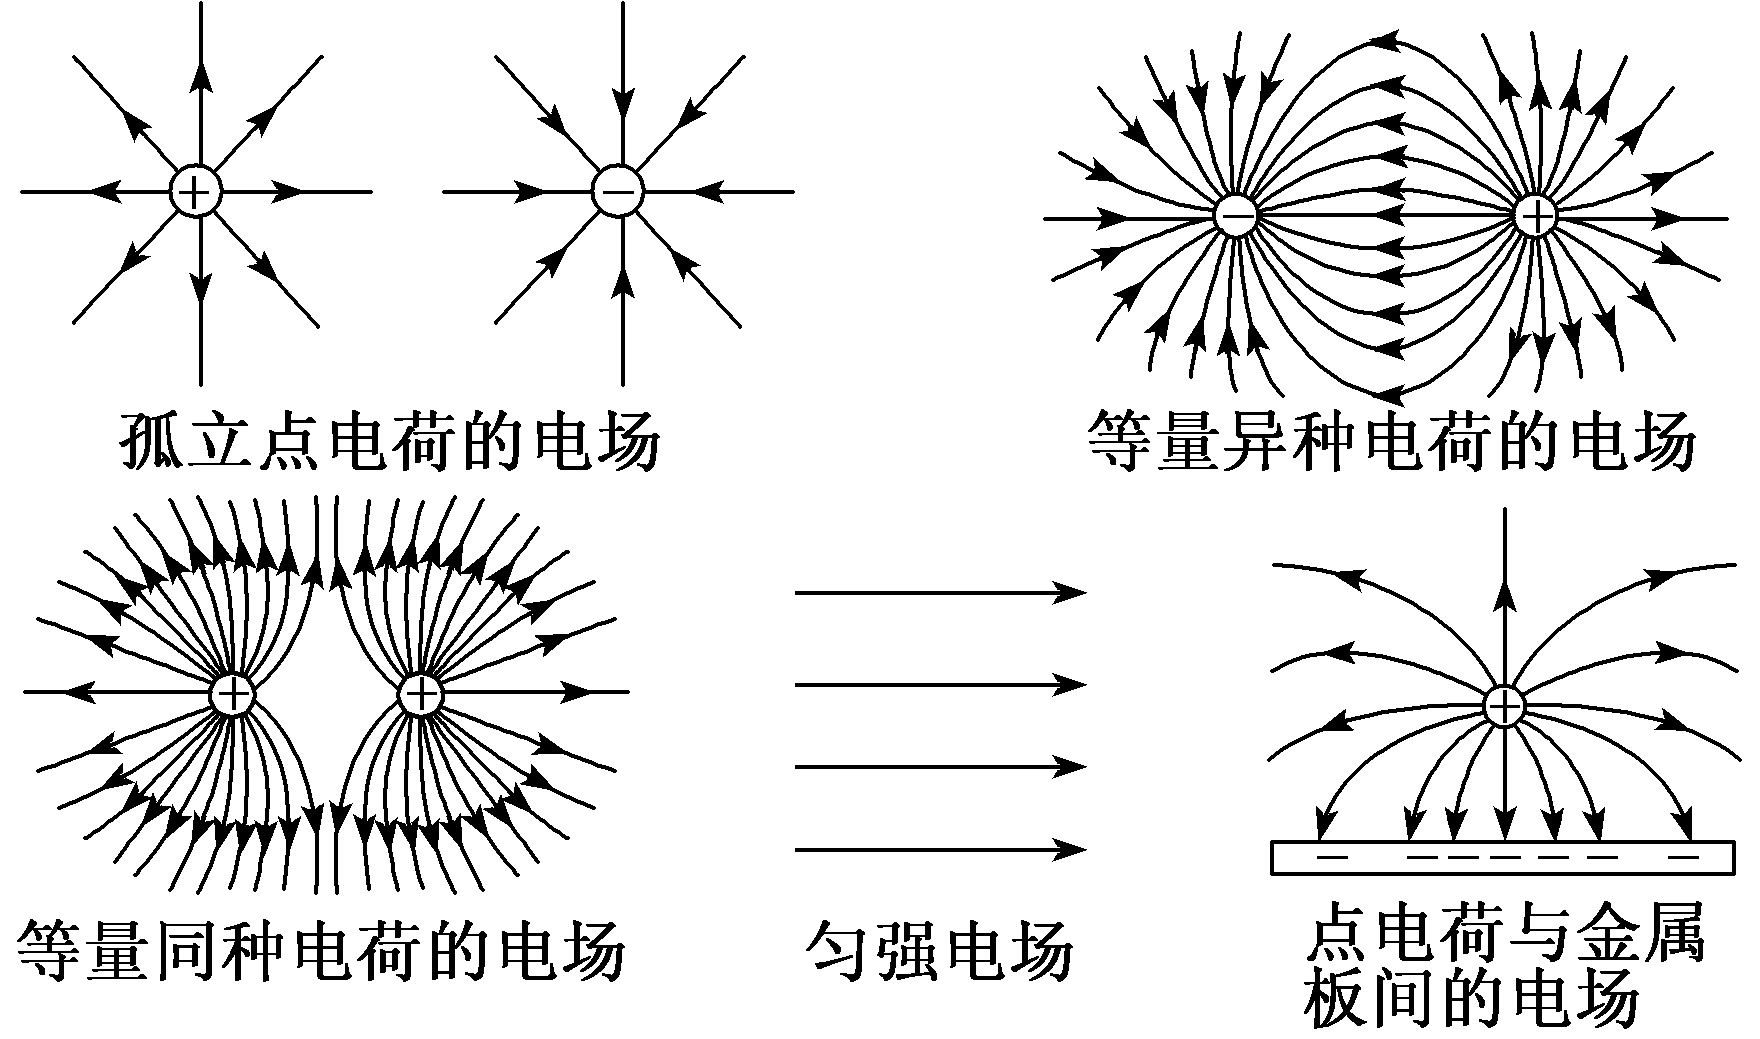
\includegraphics{./dianchang/dianchang1.png}
  \caption{六种常见的电场线}
  \label{fig:dianchangxian}
\end{figure}

在高中课本中给出了以上六种电场线的分布图,下面我们讨论一下这几个电场线的特点.

{\bf 孤立点电荷的电场}:此电场可以由公式计算.由真空中点库仑定律和电场强度的定义可得
\begin{gather}
  \left.
    \begin{gathered}
      F=k\frac{Qq}{r^2}\\
      E=\frac{F}{q}
    \end{gathered}
  \right\}
  \Longrightarrow
  E=k\frac{Q}{r^2}
\end{gather}

对于上式我们即可以按\CJKunderwave{标量式}来理解:即电荷量$Q$认为是其绝对值,而方向则单独记忆(正的点电荷激发的场强方向沿半径向外,负的点电荷激发的场强方向沿半径向里.),也可以按\CJKunderwave{矢量式}来记忆:沿半径方向向外为正,则$Q>0 , E>0$ 场强方向与正方向相同;如$Q<0,E<0$ 则场强方向与正方向相反.
\footnote{由于在电场这一部分的公式中出现的$q$ 有正电也有负电,为了不至于使用上的混乱,我建议同学位采用矢量式的方法记忆,这样今后所涉及的公式都需要$q$自身内部今有正负号,不需要再区分带不带正负号的问题.}
从公式上来看:\CJKunderwave{当r增大时,场强的大小会减小},从电场线上来看:\CJKunderwave{离点电荷越远,则电场线越稀疏,则场强的大小也越来越小},公式的描述和电场线的描述是一致的,但是电场线不能给出具体的数值,公式法可以给出具体数值,然而电场线较公式法的优点在于能够在整体上给出电场的分布情况.

{\bf 等量异种电荷的电场}:我们首先来看电场线中间连线上场强的分布情况,从电场线上来看由正电荷向负电荷电场线先变稀疏再变密集,所以场强是\CJKunderwave{先变小再变大,而且方向由正电荷指向负电荷}.这个情况,我们也可以根据电场的叠加从公式来看,如下

  设由正电荷指向负电荷方向为正,设两个电荷的距离为$2d$,设中间连线上的点距离正电荷为$r$,则中间连线上电场强度为 
  \begin{equation}
    E=k\frac{Q}{r^2}+k\frac{Q}{(2d-r)^2}
  \end{equation}

  从数学上不难判断,当半径 $r=d$ 时电场强度取得极大值.同时大家应当注意,此公式不能使 $r$ 从零开始变化,原因在于如果 $r\to 0$,则库仑公式失效,则此公式也失效,所以这时只能通过公式确定电场的变化情况和远离点电荷的电场强度大小.

  对于中垂线上电场强度的变化,从图中可以判断出来:从中间向两侧,电场强度逐渐减小.这里大家要注意,此处应当放眼整个立体空间来看,中垂线实际上是中垂面和纸面的交线,向两侧应当实指远离中点且在中垂面上.这也可以从公式上来分析.如下

  \begin{figure}[H]
    \centering
    \begin{tikzpicture}
    \draw (-2,0) circle [radius=0.2] node {\small $+$};
    \draw (2,0) circle [radius=0.2] node {\small $-$};
    \draw[dashed] (-1.7,0)--(1.7,0);
    \draw[dashed] (0,-1)--(0,2);
    \draw[dashed] (-2,0)++(30:0.2)--++(30:2.1094);
    \draw[dashed] (2,0)++(150:0.2)--++(150:2.1094);
    \draw[->,>=stealth](0,1.1547)--++(30:1) node [anchor=south] {\tiny $k\frac{Q}{r^2}$};
    \draw[dashed](0,1.1547)++(30:1)--++(-30:1);
    \draw[->,>=stealth](0,1.1547)--++(-30:1) node [anchor=north] {\tiny $k\frac{Q}{r^2}$};
    \draw[dashed](0,1.1547)++(-30:1)--++(30:1);
    \draw[->,>=stealth](0,1.1547)--++(0:1.732) node [anchor=west] {\tiny $E$};
    \draw (-2,0)++(0:0.5) arc (0:30:0.5);
    \draw (-2,0)++(15:0.6) node {\tiny $\theta$};
    \draw (0,1.1547)++(0:0.3) arc (0:30:0.3);
    \draw (0,1.1547)++(15:0.5) node {\tiny $\theta$};
    \draw[dashed](0,1.1547)++(-30:1)--++(0,1);
    \draw (-1,0) node [anchor=north] {\tiny $d$};
    \draw (-2,0)++(30:1) node [anchor=south] {\tiny $r$};
    \draw (0,1.1547) node [anchor= east] {\tiny $P$};
    \end{tikzpicture}
    \caption{等量异种电荷中垂面上的场强}
    \label{fig:dengliangyizhongdianhe}
  \end{figure}

  对于中垂线上任意一点,由电场强度的叠加可得$P$点的场强,即
  \begin{gather}
    \left.
      \begin{gathered}
	E=2k\frac{Q}{r^2}\cos\theta\\
	r=\frac{d}{\cos\theta}
      \end{gathered}
    \right\}
    \Longrightarrow
    E=2k\frac{Q}{d^2}\cos^3\theta
  \end{gather}

  当场点由中间向两侧移动时,对应$\theta$ 将会变大,当无穷远时 $\theta=90^\circ$ ,当$0^\circ <\theta <90^\circ $ 时,$\theta$ 变大则 $\cos\theta$ 是减小的,所以中垂线上由中间向两侧电场强度逐渐减小直到为0.

  {\bf 等量同种电荷的电场}:从电场线的分布情况可以判断出来,在电荷的连线上电场强度先减小后增大,在中间位置为0,越过中点后场强改变方向,然后再增大.这一点也可以从公式来看,设向右为正,场点距左侧正电荷$r$ , 两电荷间距为 $2d$,则
  \begin{equation}
    E=k\frac{Q}{r^2}-k\frac{Q}{(2d-r)^2}
  \end{equation}
  当 $r<d$ 时 $E>0$ ,随 $r$ 增大则 $E$ 减小; 当 $r=d$ 时, $E=0$; 当 $r>d$ 时, $E<0$ , 随 $r$ 增大,则 $E$ 减小.这里也应当特别注意,$r\to 0$ 时,库仑定律失效,所以这里讨论的场强也不能是紧挨场源电荷的.

  对于中垂线上电场强度的变化,从图中可以判断出来:由于中间场强为$0$ , 在无穷远处场强也为 $0$ ,但是中垂线上除这两处外不是 $0$ ,因此场强的变化应当是先增大再减小.我们可以具体算出最大场强的位置,高一的同学暂时没有学习求导函数法求极值,计算暂时可以略过,但是待数学知识完备后,一定要回来具体计算一下此最大场强.具体计算如下

  \begin{figure}[H]
    \centering
    \begin{tikzpicture}
    \draw (-2,0) circle [radius=0.2] node {\small $+$};
    \draw (2,0) circle [radius=0.2] node {\small $+$};
    \draw[dashed] (-1.7,0)--(1.7,0);
    \draw[dashed] (0,-1)--(0,2);
    \draw[dashed] (-2,0)++(30:0.2)--++(30:2.1094);
    \draw[dashed] (2,0)++(150:0.2)--++(150:2.1094);
    \draw[->,>=stealth](0,1.1547)--++(30:1) node [anchor=west] {\tiny $k\frac{Q}{r^2}$};
    \draw[dashed](0,1.1547)++(30:1)--++(150:1);
    \draw[->,>=stealth](0,1.1547)--++(150:1) node [anchor=east] {\tiny $k\frac{Q}{r^2}$};
    \draw[dashed](0,1.1547)++(150:1)--++(30:1);
    \draw[->,>=stealth](0,1.1547)--++(90:1) node [anchor=south] {\tiny $E$};
    \draw (-2,0)++(0:0.5) arc (0:30:0.5);
    \draw (-2,0)++(15:0.6) node {\tiny $\theta$};
    \draw (0,1.1547)++(150:1)++(0:0.3) arc (0:30:0.3);
    \draw (0,1.1547)++(150:1)++(15:0.5) node {\tiny $\theta$};
    \draw[dashed](0,1.1547)++(150:1)--++(1.732,0);
    \draw (-1,0) node [anchor=north] {\tiny $d$};
    \draw (-2,0)++(30:1) node [anchor=south] {\tiny $r$};
    \draw (0,1.1547) node [anchor= east] {\tiny $P$};
    \end{tikzpicture}
    \caption{等量同种电荷中垂面上的场强}
    \label{fig:dengliangtongzhongdianhe}
  \end{figure}
  对于中垂线上任意一点,由电场强度的叠加可得$P$点的场强,即
  \begin{gather}
    \left.
      \begin{gathered}
	E=2k\frac{Q}{r^2}\sin\theta\\
	r=\frac{d}{\cos\theta}
      \end{gathered}
    \right\}
    \Longrightarrow
    E=2k\frac{Q}{d^2}\cos^2\theta\sin\theta\notag
    \intertext{上式可以写成关于$\sin\theta$ 的函数,即}
    E=2k\frac{Q}{d^2}(1-\sin^2\theta)\sin\theta\notag
    \intertext{上式对$\sin\theta$ 微分,令其微分为$0$ ,则}
    \frac{d E}{d\sin\theta}=2k\frac{Q}{d^2}(1-3\sin^2\theta)=0\notag
    \intertext{解得最大电场强度出现的位置为}
    \sin\theta=\frac{\sqrt{3}}{3}\notag
  \end{gather}
    同学们注意,上式所求$\theta$ 可不是一个特殊值,它是\CJKunderdot{正弦值}为$\frac{\sqrt{3}}{3}$ 而\CJKunderdot{不是正切值}!!

  {\bf 匀强电场}:匀强电场的电场线是等间距的平行线,等间距表明电场强度大小不变,平行表明方向在任何位置都一样.如果需要计算场强,也得在平行板电容器中才行,有的题目也会借助受力平衡的问题拐个弯用定义等来求匀强电场的大小,一般而言它是给定的,然后让同学们去求解力和运动的问题.对于最后一个,真空中的点电荷和无限大平行金属板间的电场,可以借助于镜像法来求解电势再微分来得到电场强度,但是这已经超出了高中对同学们的要求,所以此处不再具体计算.有高考题,曾经考过此类问题,但是结合电场的叠加和对称性可以方便的解决,当遇到具体问题时再做分析.

  \section{电势能和电势}

  电场是我们新认识的一种物质,当电荷放入电场中时会受到力的作用,所以当将电荷从一个位置移动到另一个位置时电场力有可能做功,但是根据能量守恒定律,这就涉及到能量的转化.但是由于电荷及电场有它自己特定的特点,同时电场大多数的情况下又不是恒力,这就不能像重力那样确定重力势能.实践表明,电荷放入电场中也有势能,我们称之为电势能.但是没有经过严格的数学论证前我们还不能肯定这个结论.有的教材上类比``重力场''来说明电场和电势能,但是我要问一句,我们哪一本书上在讲解重力时提到过重力场?同学们根本没有听过重力场\footnote{至少在高中一年级是这样的,这也是我从电荷和电场本质属性来讨论问题的原因.},所以我不想那样讲解,根据前面几节学过的内容我们可以顺理成章的给出电势能.

  一种势能的存在必然表明此势能只能是位置的函数,那就是做功与路径无关,在物理学上我们称做功与路径无关的力为\CJKunderwave{保守力}.

  \subsection{静电力是保守力}

  静电力做功也与路径无关,所以它是保守力.由于电场的复杂性,我们对于任意一个电场来讲,先来考虑一个很小很小的区域,则在这一个小区域内电场几乎没有变化,可以视为匀强电场.如图\ref{fig:yuqiangdianchanglujingwufuang} 所示

  \begin{figure}[H]
    \centering
    \begin{tikzpicture}
      \foreach \y in {0,0.5,1,1.5,2}
      \draw [->,>=stealth] (0,\y)--(3,\y);
      \draw (0.25,0.25) node [anchor=east] {\tiny $A$}--(1.75,1.75) node [anchor=west] {\tiny $B$};
      \draw[dashed] (0.25,0.25)--(1.75,0.25) node [anchor=west]{\tiny $C$}--(1.75,1.75);
      \draw (0.55,0.25) arc (0:45:0.3);
      \draw (0.25,0.25)++(22.5:0.5) node {\tiny $\theta$};
      \draw (1,0.25) node [anchor=north] {\tiny $d$};
      \draw (45:1.5) node [anchor=east]{\tiny $r$};
      \draw[->,>=stealth] (0.25,0.25)--++(0:1) node [anchor=south west]{\tiny $F$};
      \draw (0.25,0.9)node [anchor=east] {\tiny $D$} --(1.75,1.9) node [anchor=west]{\tiny $G$};
      \draw [dashed] (0.25,0.2)--(0.25,1.5);
      \draw [dashed] (1.75,0.2)--(1.75,1.9);
    \end{tikzpicture}
    \caption{匀强电场做功与路径无关}
    \label{fig:yuqiangdianchanglujingwufuang}
  \end{figure}

  我们将电荷 $q$ 沿路径 $AB$ 由 $A$ 移动到 $B$ ,计算静电力做功,则
  \begin{equation}
    W_{AB}=qEr\cos\theta
    \label{eq:jdlwork0}
  \end{equation}
  然后,我们再沿路径 $A\to C\to B$ 将电荷 $q$ 由 $A$ 移动到 $B$,计算静电力做功,则
  \begin{equation}
    W_{AB}'=W_{AC}+W_{CB}=qEd+0
    \label{eq:jdlwork1}
  \end{equation}
  对比式 \eqref{eq:jdlwork0} 和 \eqref{eq:jdlwork1} 由几何关系可得 $r\cos\theta  =d$ 所以有
  \begin{equation}
    W_{AB}=W_{AB}'
    \label{eq:jdlwork2}
  \end{equation}
  上式表明:\CJKunderwave{匀强电场中,静电力做功与路径无关.}同理也可以确定将电荷沿$DG$ 路径由 $D$ 移动到 $G$ ,静电力做功也等于$W_{AB}'$ .所以有
  \begin{equation}
    W_{AB}=W_{DG}
    \label{eq:jdlwork3}
  \end{equation}
  式 \eqref{eq:jdlwork3} 可得:在匀强电场中,只要两点沿\CJKunderwave{沿电场线方向的距离相等},则电场对电荷做功相等.

  对于一般的情况,如图 \ref{fig:yibanjdlwork},我们将路径沿电场线方向做出一定划分,每一个小区域可以视为匀强电场.路径$A\to D\to B$ 和路径 $A\to C\to B$ 离的非常近,所以按图中每隔一小段画一小条虚线与电场线(电场线未画出)垂直,由匀强电场的第二条规律:\CJKunderwave{在匀强电场中,只要两点沿沿电场线方向的距离相等,则电场对电荷做功相等.}可得第一小段上静电力做功相等,所以沿路径$A\to C\to B$ 和路径 $A\to D\to B$计算静电力做功是相同的,如果两条路径相隔比较远,则可以通过若干相邻路径逐步得到,所以可以断言:任何静电场中,静电力做功与路径无关,只取决于始末位置.


  \begin{figure}[H]
    \centering
    \begin{tikzpicture}
      \draw (0,0) node [anchor=east] {\tiny $A$}--++(60:0.5)--++(50:0.5) node [anchor= south east] {\tiny $C$}--++(40:0.5)--++(30:0.5) node [anchor=west] {\tiny $B$};
      \draw (0,0)--++(30:0.5)--++(40:0.5) node [anchor=west] {\tiny $D$}--++(50:0.5)--++(60:0.5);
      \draw[dashed] (20:0.5) arc (20:80:0.5) node [anchor=east] {\tiny 1};
      \draw[dashed] (20:1) arc (20:60:1) node [anchor=east] {\tiny 2};
      \draw[dashed] (20:1.5) arc (20:60:1.5) node [anchor=east] {\tiny 3};
    \end{tikzpicture}
    \caption{一般电场的情况}
    \label{fig:yibanjdlwork}
  \end{figure}

  \subsection{电势能}
  由于静电力是保守力,所以由静电力做功与路径无关可以判断静电力做功只与始末位置有关,这是上一节的结论.由于$W_{AB}$ 只与始末位置有关,所以它可以表达为两个函数的差的形式,这个函数我们就称为电势能.即
  \begin{equation}
    W_{AB}=E_{pA}-E_{pB}
    \label{eq:dianshineng}
  \end{equation}

  式\eqref{eq:dianshineng}将\CJKunderwave{静电力做功表达为电势能的减少量},但是具体的电势能的数值还没有确定下来,这就需要人为的选定.由式\eqref{eq:dianshineng} 可以得出,如果我们选定 $E_{pB}=0 J$ ,则
  \begin{equation}
    E_{pA}=W_{AB}
    \label{eq:dianshineng1}
  \end{equation}
  式\eqref{eq:dianshineng1}可得一条重要的结论:\CJKunderwave{某点的电势能等于将电荷从该点移动到零势能点静电力做的功.}

  \subsection{电势}

  不同的电荷放在同一个电场中的相同位置,它们的受力是不一样的,所以移动时静电力做功也不一样,则电势能也不相同.所以可以判断电势能与电荷量有关,不能表示电场自身的性质,同时由于电场的多样性,也不可能找出一个和重力势能一样的简单的表达式.但是电荷它有自己的特点,即:\CJKunderwave{所有的电荷量都是元电荷的整数倍}. 由于这个特点,我们可将电荷 $q$ 从 $A$ 点移动到 $B$ 点计算电场力做功时,可以一次性的移动过去,也可以分成若干次,每次只移动一个元电荷$e$ ,于是可以得出结论:\CJKunderwave{从 $A$ 到 $B$ 静电力做功与移动的次数成正比,同时由电势能的定义可以断定电势能也与这个移动次数成正比,}即设移动次数为 $N$ ,则 $N=\frac{q}{e}$,所以可以得出 $E_p$ 和电荷量 $q$ 成正比,定义此比例系数为\CJKunderwave{电势},使用符号$\varphi$ \footnote{$\varphi$ 是希腊字母,同学们要准确的书写不要与英文字母弄混,这点特别引起注意.}表示,则其定义为
  \begin{equation}
    \varphi=\frac{E_p}{q}
    \label{eq:dianshi}
  \end{equation}
  式\eqref{eq:dianshi} 表明,电势是一个标量,符合比值定义法,其不依赖于电场中所放置的电荷,所以电势可以表征\CJKunderwave{电场自身的属性}.对于比值定义法,在这里有必要解释一下,因为平时的教学中很多学生总是在这里出问题.举一例来说明,比如远古时代并没有钱,但是随着社会发展出现了货币,也就是钱!但是由于钱的特殊作用,以及重要性,人们需要专门的找一个包来存放它,慢慢的大家就给放钱的这个包起了一个名字---钱包.这里你看,钱包是用钱来定义的,但是它和钱绝对不是一个东西,而且一个钱包的存钱能力(容积大小)和它里面有没有钱也是没有关系的!所以电势虽然是由电荷放入电场中时所具有的电势能和电荷量的比值来定义的,但它和放入其中的电荷是没有关系的,所以它代表了电场自身能的性质! 如果我们再深入一些找一下决定电势的因素,则电场是由场源电荷激发的,所以它取决于场源电荷,同时电场一定的情况下,电势也不是确定的,因为还需要人为的指定零电势能的位置(也可以说是零电势位置).

  电势是一个标量,它的单位是:伏特,符号为 V .\footnote{大家注意,这里的伏特就是初中时大家学习的电压的单位,但是电势又不是电压,这需要在后面的课程中解释.}

  \section{电势差}

  前面我们介绍了电势能的概念和电势的概念,但是在计算一般情况下静电力做功时,并不总是很实用,原因在于如果每次计算都先选择零势能面,会带来不必要的计算.考虑到这个因素,我们引入一个新的物理量---电势差.定义如下
  \begin{equation}
    U_{AB}=\varphi_A-\varphi_B
    \label{eq:dianshicha}
  \end{equation}

  注意定义\eqref{eq:dianshicha} 中下脚标的顺序,$AB$不能颠倒.由这定义可以得到下面的二个性质
  \begin{gather}
    U_{AB}=-U_{BA}\\
    U_{AC}=U_{AB}+U_{BC}
  \end{gather}
  上述性质是显然的,由电势差的定义不难证明,这里留给同学们自己完成证明,不再辍述.

  我们再来讨论一下静电力做功与电势差的关系.如下
  \begin{gather}
    \left.
    \begin{gathered}
    W_{AB}=E_{pA}-E_{pB}\\
    E_p=q\varphi\\
    U_{AB}=\varphi_A-\varphi_B
    \end{gathered}
  \right\}
  \Longrightarrow
  U_{AB}=\frac{W_{AB}}{q}
  \label{eq:WandU}
  \end{gather}

  关系式 \eqref{eq:WandU} 可以用来知道电势差的情况下直接计算功,也可以知道功的情况下直接计算电势差,由于它不涉及零势能面的选择,所以使用起来比较方便.

  \section{电场强度和电势差的关系}

  现在讨论一个特殊,在匀强电场中电场力是恒力,所以它做的功可以直接算出,因而可以得到一个非常好用的关系式.在讨论匀强电场中静电力做功的时候我们得到从$A$ 到 $B$ 静电力做功为$W_{AB}$,$d$ 表示沿电场线方向 $AB$ 的距离.将其应用于电势差的计算式中,即
  \begin{gather}
    \left.
      \begin{gathered}
	W_{AB}=qEd \\
	U_{AB}=\frac{W_{AB}}{q}
      \end{gathered}
    \right\}
    \Longrightarrow
    U_{AB}=Ed
    \label{eq:EanU}
  \end{gather}
  为了更好的理解方向和它们之间的关系,我们沿电场线方向建立一维直线坐标系,则如图\ref{fig:PhiAndE}所示,由电势差的定义,我们可以把场强与电势差的关系写为
  \begin{equation}
    E=-\frac{\varphi_B-\varphi_A}{x_B-x_A}=-\frac{\Delta\varphi}{\Delta x}
    \label{eq:EandU1}
  \end{equation}
\begin{figure}[H]
  \centering
  \begin{tikzpicture}
    \foreach \y in {0,0.5,1,1.5,2}
    \draw [->,>=stealth] (0,\y)--(3,\y);
    \draw (3.5,1) node {\small $E$};
    \draw [->,>=stealth] (-1,0.75)--(4,0.75) node [anchor=west] {\small $x$};
    \filldraw (1,0.75) node [anchor=south] {\tiny $A$} circle [radius=1pt];
    \filldraw (2,0.75) node [anchor=south] {\tiny $B$}circle [radius=1pt];
  \end{tikzpicture}
  \caption{电场强度与电势差的关系}
  \label{fig:PhiAndE}
\end{figure}

\section{电容器的电容}

我们学习了起电的方式,找到了能够得到净电荷的方法.但是由于开始并不清楚电荷及电场的有关特点,所以尚没有解决电荷存储的问题.这一节所解决的就是电荷存储的问题.\CJKunderwave{能够存储电荷的\CJKunderdot{设备}叫做\CJKunderdot{电容器}}.电容器存储电荷的基本原理是:异种电荷相互吸引.如果将两个导体之间充以绝缘介质,则当两个导体上分别使其带上异种电荷时,由于异种电荷间的相互吸引,同时它们之间又是绝缘的,电荷还不能中和,所以最后只能分别在两个导体上了,而且最终也必然会保持电荷在宏观上的静止状态.
\begin{figure}[H]
  \centering
  \begin{tikzpicture}
    \draw (-0.2,0) rectangle (3.2,0.2); 
    \draw (-0.2,2) rectangle (3.2,2.2); 
    \foreach \x in {0,0.5,1,1.5,2,2.5,3}
    \draw (\x, 0.1) node {\tiny $-$};
    \foreach \x in {0,0.5,1,1.5,2,2.5,3}
    \draw (\x, 2.1) node {\tiny $+$};
    \foreach \x in {0,0.5,1,1.5,2,2.5,3}
    \draw[->,>=stealth] (\x,1.95) -- (\x, 0.25);
    \draw (1.5,1.1) node {\small 绝缘介质};
  \end{tikzpicture}
  \caption{平行板电容器}
  \label{fig:pingyxingban}
\end{figure}

如图 \ref{fig:pingyxingban} 所示,是最简单的一种电容器,它有两个无限大金属板中间填充绝缘介质构成,所以叫做平行板电容器.如果我们将两个极板同时和电源的正负两极连接,则两个极板上就会充上等量异种电荷,我们把这个过程叫做电容器的充电.图中正是表示的充电后的状态.如果我们把一个充电的电容器的两极用一根导线连接,则正负电荷就会通过导线中和,从而二个极板不再带电,我们称这个过程为电容器的放电.由这个特点我们可以肯定的是电容器的容量是指\CJKunderwave{一个极板上的电荷量的绝对值.}

就像水杯一样,水杯是盛水的容器,不同的水杯有不同的容积,也就是有不同的水的容纳能力.电容器也是一样,不同的电容器对电荷的容纳能力也是不一样的,所以就产生了如何衡量电容器电荷容纳能力的问题.当有电场时,即便是绝缘介质,它不导电,但是由于原子是电中性,电场会使其中的正负电荷向相反的方向偏离,但是由于原子内部正负电荷的吸引,最终会和外部的电场力平衡掉.但是确改变了原子的形状!原则上讲,只要是外电场足够强大,就能使绝缘介质的原子中的正负电荷分开,我们称之为电离.因此,只有在绝缘介质不发生电离时,电容器才是完好的,其两个极板上的电荷才不会中和,而得以存储.所以这里就存在一个电容器中所能允许的最大场强问题,也就是电场线的密度不能超过一个值,然而电荷又都是元电荷的整数倍,所以可以认为每一个元电荷对就一条电场线,由于电场线的条数在正对面积一定的情况下有一个极大值,则一个极板上的电荷量也必然有一个极大值,也就是说电容器极板上的电荷量也是有限制的.同时根据 
$U=Ed$ 可得,在两板间距离 $d$ 一定的情况下,电压也是存在一个上限的,我们称之为额定电压.

当一个电容器制成后,如果增加极板上的电荷量,则极板间的电压也跟着增加,同时场强也增加,但是如果两个电容器充以相同的电介质,当增加相同的电量时,增加电压少的那一个意味着电场强度增加的也少,意味着更不容易导致介质电离,也就是电荷容纳本领越大.所以可以使用电荷量与板间电压的比值来表示电容器容纳电荷的本领,定义为电容,即
\begin{equation}
  C=\frac{Q}{U}
  \label{eq:dianrong}
\end{equation}
由定义可知,电容是一个标量.电容的国际单位是:法拉,符号为:$F$. 法拉是一个极大的单位,日常中常见电容器的电容一般都达不到这么大,所认还有两个更小的单位皮法$pF$ 和微法 $\mu F$,它们之间的进位为
\begin{equation}
  1F=10^6 pF = 10^{12} \mu F
  \label{eq:falajinwei}
\end{equation}

综上讨论,我们可以得出一些结论,在一个极板上电荷量一定的情况下,如果正对面积越大,则电场线密度越低,则电容器容纳电荷的本领越大.同时在相同介质的前提下,两个极板间距离越大则两个电荷间的库仑力越小,则保持电荷稳定保存的能力就越低,所以板间距离越大,则电容器容纳电荷的本领就越小.同时电容器不易电离的能力,也即是绝缘能力越大则该电容器的容纳电荷的本领越大.以 $S$ 表示极板正对面积, 以 $d$ 表示板间距离, 以 $\varepsilon_r$ 表示相对介电常数\footnote{$\varepsilon$ 为介质的介电常数, $\varepsilon_0$ 为真空中的介电常数,相对介电常数定义为 $\varepsilon_r=\frac{\varepsilon}{\varepsilon_0}$ ,它们是衡量物质绝缘性能的物理量,其值越大,则绝缘性能越好.},所以我们可以推断出来平行板电容器的电容和正对面各成正比,和板间距离成反比,和相对介电常数成正比,即 $C\propto \frac{\varepsilon_r S}{d}$ ,严格计算的结果为
\begin{equation}
  C=\frac{\varepsilon_r S}{4\pi k d}
  \label{eq:dianrongpingban}
\end{equation}
上式中$k$ 为静电力常量,其值为$k=9.0\times 10^9 N\cdot m^2/C^2$.
\section{带电粒子在电场中的运动}

\subsection{带电粒子的加速}

当带电粒子在电场中运动时,高中最常处理的也是最基本的就是带电粒子的加速问题.如图
\ref{fig:ddlzjiasu}所示,两板间电压为$U_1$, 平行板间距离为$d_1$,粒子的带电量为$q$,质量为$m$.

\begin{figure}[H]
  \centering
  \begin{tikzpicture}
    \draw (-0.2,-1.5) rectangle (0,1.5); 
    \draw (2,-1.5) rectangle (2.2,-0.05); 
    \draw (2,0.05) rectangle (2.2,1.5); 
    \foreach \y in {-1.4,-1.0,-0.6,-0.2,0.2,0.6,1.0,1.4}
    \draw (-0.1,\y) node {\tiny $+$};
    \foreach \y in {-1.4,-1.0,-0.6,-0.2,0.2,0.6,1.0,1.4}
    \draw (2.1,\y) node {\tiny $-$};
    \foreach \y in {-1.4,-1.0,-0.6,-0.2,0.2,0.6,1.0,1.4}
    \draw[->,>=stealth] (0.1,\y)--(1.9,\y);
    \filldraw (0.1,0) circle [radius=1pt] node [anchor=south]{\tiny $q$};
    \filldraw (2.3,0) circle [radius=1pt] node [anchor=south]{\tiny $q$};
    \draw[->,>=stealth] (2.35,0)--(2.75,0) node [anchor=west]{\tiny $v_0$};
    \draw[color=white](-1.55,0)--(0,0);
  \end{tikzpicture}
  \caption{带电粒子在电场中加速}
  \label{fig:ddlzjiasu}
\end{figure}

下面我们来求带电粒子离开加速电场时的速度$v_0$,由动能定理得
\begin{gather}
  qU=\frac{1}{2}mv_0^2
  \intertext{解得}
  v_0=\sqrt{\frac{2qU_1}{m}}
  \intertext{如果要求粒子的加速时间,则需要考虑运动学公式,由平均速度公式得}
  d_1=\frac{v_0}{2}t
  \intertext{解得}
  t=\frac{2d_1}{v_0}=d_1\cdot\sqrt{\frac{2m}{qU_1}}
  \intertext{此题也可以由匀变速直线运动来求解.由牛顿第二定律得}
  q\frac{U_1}{d_1}=ma_1
  \intertext{解得}
  a_1=\frac{qU}{md_1}
  \intertext{由匀变速直线运动位移与时间的关系可得}
  d_1=\frac{1}{2}a_1t^2
  \intertext{解得}
  t=\sqrt{\frac{2d_1}{a_1}}=d_1\cdot\sqrt{\frac{2m}{qU_1}}
\end{gather}

\subsection{带电粒子在电场中的偏转}

这一节讨论带电粒子在电场中的偏转问题,由于高中的要求,此处仅讨论类平抛运动.如图\ref{fig:ddlzpz}所示,两板间电压为$U_2$,板长为$L$.

\begin{figure}[H]
  \centering
  \begin{tikzpicture}
    \draw (-2,-1.7) rectangle (2,-1.5); 
    \draw (-2,1.7) rectangle (2,1.5); 
    \draw[dashed] (-2,0)--(2,0);
    \draw[domain=-2:2] plot (\x,-\x*\x/12-\x/3-1/3);
    \draw[->,>=stealth] (-2,0)--(-1,0) node [anchor=south]{$v_0$};
    \filldraw (-2,0) circle [radius=2pt];
    \draw[dashed](0,0)--(2,-1.333);
    \filldraw (2,-1.333) circle [radius=2pt];
    \draw[->,>=stealth] (2,-1.333)--++(1,-0.666) node [anchor=west]{\small $v$};
    \draw[->,>=stealth] (2,-1.333)--++(1,0) node [anchor=south]{\small $v_x$};
    \draw[->,>=stealth] (2,-1.333)--++(0,-0.666) node [anchor=east]{\small $v_y$};
    \draw[dashed](2,-1.333)++(1,0)--++(0,-0.666);
    \draw[dashed](2,-1.333)++(0,-0.666)--++(1,0);
    \draw[dashed](-2,0)--(2,-1.333);
    \draw (-2,0)++(0.6,-0.1998) arc (-18.433:0:0.6);
    \draw (-2,0)++(-9.22:0.8) node {\small $\alpha$};
    \draw(2,-1.333)++(-33.6874:0.4) arc (-33.6874:0:0.4);
    \draw(0,0)++(-33.6874:0.4) arc (-33.6874:0:0.4);
    \draw(2,-1.333)++(-16.8437:0.6) node {\small $\theta$}; 
    \draw(0,0)++(-16.8437:0.6) node {\small $\theta$}; 
    \draw (0,1.5) node [anchor=north]{\small $L$};
    \draw (-2.3,1.5)--(-2.1,1.5);
    \draw (-2.3,-1.5)--(-2.1,-1.5);
    \draw[dashed] (-2.2,-1.5)--(-2.2,1.5);
    \draw (-2.2,0) node [anchor=east]{$d$};
    \draw (2.1,0)--(2.3,0);
    \draw (2.1,-1.333)--(2.3,-1.333);
    \draw[dashed](2.2,0)--(2.2,-1.333);
    \draw (2.3,-0.666) node {\small $y$};
  \end{tikzpicture}
  \caption{带电粒子在电场中偏转}
  \label{fig:ddlzpz}
\end{figure}

\subsubsection{偏转加速度}

由牛顿第二定律可得
\begin{gather}
  q\frac{U_2}{d}=ma_2
  \intertext{解得}
  a_2=\frac{qU_2}{md}
  \label{eq:ddpya}
\end{gather}
上述结果同学位要记住,它很有规律,而且一旦记住能够实现快速写出偏转问题中的偏移量和偏转角等.

\subsubsection{偏移量}

图\ref{fig:ddlzpz} 中所示,带电粒子射出电场时相对于入射方向的纵向位移就叫做偏移量.由运动的独立性可得运动的时间为
\begin{gather}
  t=\frac{L}{v_0}
  \label{eq:ddpyl0}
  \intertext{所以偏移量为}
  y=\frac{1}{2}a_2t^2
  \label{eq:ddpyl1}
  \intertext{将式\eqref{eq:ddpya}和\eqref{eq:ddpyl0}代入\eqref{eq:ddpyl1}后得}
  y=\frac{1}{2}\cdot\frac{qU_2}{md}\cdot\frac{L^2}{v_0^2}
  \label{eq:ddpyl2}
\end{gather}

\subsubsection{位移偏转角}

由图\ref{fig:ddlzpz} 可得位移的偏转角为
\begin{gather}
  \tan\alpha=\frac{y}{L}=
  \frac{1}{2}\cdot\frac{qU_2}{md}\cdot\frac{L}{v_0^2}
  \label{eq:ddpyl3}
\end{gather}

\subsubsection{出射速度}

由运动学公式可得
\begin{gather}
  v_y=a_2t=\frac{qU_2}{md}\cdot\frac{L}{v_0}
  \intertext{由运动的合成可得}
  v=\sqrt{v_0^2+v_y^2}
  \intertext{这个出射速度也可以由动能定理求得,即}
  q\frac{U_2}{d}y=\frac{1}{2}mv^2-\frac{1}{2}mv_0^2
\end{gather}
 但是请同学们注意,在已经求得运动的时间和加速度的前提下,此处的动能定理走了弯路,原因在于偏移量本来就是由运动学公式求出来的,再代入动能定理运算会增加计算量.所以直接由运动的合成来求更方便.

\subsubsection{出射速度偏转角}

由图\ref{fig:ddlzpz} 及运动的合成和分解可得
\begin{gather}
  \tan\theta=\frac{v_y}{v_0}=\frac{qU_2}{md}\cdot\frac{L}{v_0^2}  
  \label{eq:ddpyl4}
\end{gather}

\subsubsection{位移偏转角和速度偏转角的关系}

对比式\eqref{eq:ddpyl4}和式\eqref{eq:ddpyl3}可得二个偏转角的正切值满足二倍关系.

\begin{gather}
  \tan\theta=2\tan\alpha
\end{gather}
注意:此处的二倍关系在平抛运动的计算中出现过.这是一个数学结论,只要轨迹是二次曲线,则它的切线与$x$轴的交点就是二次曲线顶点到所求切线的这一点的中点.可以证明如下:

\begin{figure}[H]
  \centering
  \begin{tikzpicture}
    \draw[->,>=stealth] (-2,0)--(2,0) node [anchor=north]{\small $x$}; 
    \draw[->,>=stealth] (0,-1)--(0,2) node [anchor=east]{\small $y$}; 
    \draw[domain=-1.4:1.4] plot (\x,\x*\x);
    \draw[dashed](1.2,1.44)--(1.2,0);
    \draw[dashed](1.2,1.44)--(0,1.44);
    \draw (0.6,0)--(1.2,1.44)--++(0.2,0.48);
    \draw (0.6,0)++(0.3,0) arc (0:67.38:0.3);
    \draw (0.6,0)++(33.69:0.5) node {\small $\theta$};
    \draw (1.2,0) node [anchor=north]{\small $x$};
    \draw (0.6,0) node [anchor=north]{\small $x_0$};
    \draw (0,1.44) node [anchor=east]{\small $x^2$};
    \draw (0,0) node [anchor=north east]{\small $O$};
    \draw (-1.2,1.44) node [anchor=east]{\small $y=x^2$};
  \end{tikzpicture}
  \caption{二倍关系论证}
  \label{fig:twobei}
\end{figure}
数学上容易求得切线的斜率,即对函数求导数
\begin{gather}
  \tan\theta=y'=2x
  \intertext{反向延长切线,交$x$轴于$x_0$,则由几何关系可得}
  \tan\theta=\frac{x^2}{x-x_0}
  \intertext{二者联立求得}
  x_0=\frac{1}{2}x
\end{gather}
所以$x_0$就是顶点$O$和坐标点$x$的中点.
\subsection{带电粒子加速和偏转的联合作用}
当一个粒子依次通过加速电场和偏转电场时,会有一些特殊的规律.这一节讨论这些特点.如图\ref{fig:ddlzjspz}所示,设加速电压为$U_1$,偏转电压为$U_2$.

\begin{figure}[H]
  \centering
  \begin{tikzpicture}
    \draw (-2,-1.7) rectangle (2,-1.5); 
    \draw (-2,1.7) rectangle (2,1.5); 
    \draw[dashed] (-2,0)--(2,0);
    \draw[domain=-2:2] plot (\x,-\x*\x/12-\x/3-1/3);
    \draw[->,>=stealth] (-2,0)--(-1,0) node [anchor=south]{$v_0$};
    \filldraw (-2,0) circle [radius=2pt];
    \draw[dashed](0,0)--(2,-1.333);
    \filldraw (2,-1.333) circle [radius=2pt];
    \draw[->,>=stealth] (2,-1.333)--++(1,-0.666) node [anchor=west]{\small $v$};
    \draw[->,>=stealth] (2,-1.333)--++(1,0) node [anchor=south]{\small $v_x$};
    \draw[->,>=stealth] (2,-1.333)--++(0,-0.666) node [anchor=east]{\small $v_y$};
    \draw[dashed](2,-1.333)++(1,0)--++(0,-0.666);
    \draw[dashed](2,-1.333)++(0,-0.666)--++(1,0);
    \draw[dashed](-2,0)--(2,-1.333);
    \draw (-2,0)++(0.6,-0.1998) arc (-18.433:0:0.6);
    \draw (-2,0)++(-9.22:0.8) node {\small $\alpha$};
    \draw(2,-1.333)++(-33.6874:0.4) arc (-33.6874:0:0.4);
    \draw(0,0)++(-33.6874:0.4) arc (-33.6874:0:0.4);
    \draw(2,-1.333)++(-16.8437:0.6) node {\small $\theta$}; 
    \draw(0,0)++(-16.8437:0.6) node {\small $\theta$}; 
    \draw (0,1.5) node [anchor=north]{\small $L$};
    \draw (2.1,0)--(2.3,0);
    \draw (2.1,-1.333)--(2.3,-1.333);
    \draw[dashed](2.2,0)--(2.2,-1.333);
    \draw (2.3,-0.666) node {\small $y$};
    \draw (-2.1,-1.7) rectangle (-2.2,-0.1);
    \draw (-2.1,1.7) rectangle (-2.2,0.1);
    \draw (-4.1,-1.7) rectangle (-4,1.7);
    \filldraw (-3.9,0) circle [radius=2pt] node [anchor=south]{\small $q$};
  \end{tikzpicture}
  \caption{带电粒子的加速和偏转}
  \label{fig:ddlzjspz}
\end{figure}

\subsubsection{偏移量}

由加速电场中的动能定理得
\begin{gather}
  qU_1=\frac{1}{2}mv_0^2
  \intertext{偏转电场中的偏移量已经计算出来为}
  y=\frac{1}{2}\frac{qU_2}{md}\frac{L^2}{v_0^2}
  \intertext{上稍加整理,将$mv_0^2$视为一个整体,代入动能定理更加方便.注意大家不要求出$v_0$后再代入$v_0$,因为那样就走了弯路.我们需要的是$mv_0^2$这个整体代换,即}
  y=\frac{1}{2}\frac{qU_2L^2}{d\cdot mv_0^2}
  =\frac{1}{2}\frac{qU_2L^2}{d\cdot 2qU_1}\notag
  \intertext{简单计算可得}
  y=\frac{U_2}{U_1}\cdot \frac{L^2}{4d}
\end{gather}
大家注意,在上面的结果中,偏移量与带电粒子的电量及质量都没有关系,所以\CJKunderwave{无论是什么样的粒子经过这一装置后,它的偏移量都是相同的.}

\subsubsection{位移偏转角}

由图\ref{fig:ddlzjspz}可得,位移的偏转角为
\begin{gather}
  \tan\alpha=\frac{y}{L}=\frac{U_2}{U_1}\cdot \frac{L}{4d}
\end{gather}
上式表明,位移偏转角也与粒子的电量和质量无关.

\subsubsection{速度偏转角}

由速度与入射方向偏转角的正切值是位移偏转角正切值的二倍关系可得
\begin{gather}
 \tan\theta=2\tan\alpha= \frac{U_2}{U_1}\cdot \frac{L}{2d}
\end{gather}
上式表明,速度偏转角也与粒子的电量和质量无关.

\subsubsection{屏幕上的偏移量}

设屏幕距离出射电场右极板的水平距离为$L_0$,由于出射粒子速度反向沿长线过极板中点,这就像粒子直接从极板的中点位置沿直线发射出来一样.这样考虑时,计算屏幕上的偏移量是最简单的.如图\ref{fig:ddlzjspzpm}所示

\begin{figure}[H]
  \centering
  \begin{tikzpicture}
    \draw (-2,-1.7) rectangle (2,-1.5); 
    \draw (-2,1.7) rectangle (2,1.5); 
    \draw[dashed] (-2,0)--(2,0);
    \draw[domain=-2:2] plot (\x,-\x*\x/12-\x/3-1/3);
    \draw[->,>=stealth] (-2,0)--(-1,0) node [anchor=south]{$v_0$};
    \filldraw (-2,0) circle [radius=2pt];
    \draw[dashed](0,0)--(2,-1.333);
    \filldraw (2,-1.333) circle [radius=2pt];
    \draw[->,>=stealth] (2,-1.333)--++(1,-0.666) node [anchor=west]{\small $v$};
    \draw[->,>=stealth] (2,-1.333)--++(1,0) node [anchor=south]{\small $v_x$};
    \draw[->,>=stealth] (2,-1.333)--++(0,-0.666) node [anchor=east]{\small $v_y$};
    \draw[dashed](2,-1.333)++(1,0)--++(0,-0.666);
    \draw[dashed](2,-1.333)++(0,-0.666)--++(1,0);
    \draw[dashed](-2,0)--(2,-1.333);
    \draw (-2,0)++(0.6,-0.1998) arc (-18.433:0:0.6);
    \draw (-2,0)++(-9.22:0.8) node {\small $\alpha$};
    \draw(2,-1.333)++(-33.6874:0.4) arc (-33.6874:0:0.4);
    \draw(0,0)++(-33.6874:0.4) arc (-33.6874:0:0.4);
    \draw(2,-1.333)++(-16.8437:0.6) node {\small $\theta$}; 
    \draw(0,0)++(-16.8437:0.6) node {\small $\theta$}; 
    \draw (0,1.5) node [anchor=north]{\small $L$};
    \draw[dashed](2,0)--(2,-1.333);
    \draw (2,-0.666) node [anchor=west] {\small $y$};
    \draw (-2.1,-1.7) rectangle (-2.2,-0.1);
    \draw (-2.1,1.7) rectangle (-2.2,0.1);
    \draw (-4.1,-1.7) rectangle (-4,1.7);
    \filldraw (-3.9,0) circle [radius=2pt] node [anchor=south]{\small $q$};
    \filldraw (4,-2.8) rectangle (4.1,2.8);
    \draw[dashed] (2,-1.333)--(4,-2.666);
    \draw[dashed] (2,0)--(4,0);
    \draw (2,0)--(2,0.2);
    \draw (2,0.1)--(4,0.1);
    \draw (3,0) node [anchor=south]{\small $L_0$};
    \draw (0,0)--(0,0.2);
    \draw (0,0.1)--(2,0.1);
    \draw (1,0) node [anchor=south] {\small $\frac{L}{2}$};
    \draw (4.1,0)--(4.3,0);
    \draw (4.1,-2.666)--(4.3,-2.666);
    \draw[dashed] (4.2,0)--(4.2,-2.666);
    \draw (4.2,-1.333) node [anchor=west]{\small $Y$};
  \end{tikzpicture}
  \caption{屏幕上的偏移量}
  \label{fig:ddlzjspzpm}
\end{figure}

由几何关系很容易得出这个屏幕上的偏移量为
\begin{gather}
Y=(\frac{L}{2}+L)_0)\tan\theta=(\frac{L}{2}+L_0)\cdot\frac{U_2}{U_1}\cdot\frac{L}{2d}
\end{gather}

\chapter{恒定电流}
\section{电流}

电荷的定向移动形成电流.其定义为:单位时间通过横截面的电量.设$\Delta t$时间内通过横截面的电荷量为$\Delta Q$,即
\begin{equation}
  I=\frac{\Delta Q}{\Delta t}
  \label{eq:dianliu}
\end{equation}

电流的单位是{\bf 安培},符号为{\bf $A$},它是一个标量,但是有方向.我们规定\CJKunderwave{正电荷定向移动的方向}为电流的方向.大家注意,电流是有大小和方向,但是它的方向指的是从空间固定的$A$点向固定的$B$点流动,它不能像速度那样使用平行四边形定则合成或分解,所以它\CJKunderwave{不是矢量}.

如图\ref{fig:dianliu0}所示,图中 \tikz{\filldraw (0,0) circle [radius=2pt];} 表示定向移动的正电荷,经过$\Delta t$ 电荷通过横截面(图中虚线)的电荷量就是$\Delta Q$,电流的定义就是它们的比值.
\begin{figure}[H]
  \centering
  \begin{tikzpicture}
    \draw (-2,-1) rectangle (2,1); 
    \draw[dashed] (0,-1.2)--(0,1.2);
    \foreach \x in {-0.2,-0.5,-0.8,-1.1,-1.4,-1.7}
    \foreach \y in {-0.75,-0.45,-0.15,0.15,0.45,0.75}
    \filldraw (\x,\y) circle [radius=2pt];
    \draw (0,-1.5) node [anchor=north] {\small $t$时刻};
    \draw[->,>=stealth] (0,0)--++(0.5,0);
  \end{tikzpicture}
  \qquad
  \begin{tikzpicture}
    \draw (-2,-1) rectangle (2,1); 
    \draw[dashed] (0,-1.2)--(0,1.2);
    \foreach \x in {-1.7,-1.4,-1.1,-0.8,-0.5,-0.2,0.1,0.4,0.7,1,1.3}
    \foreach \y in {-0.75,-0.45,-0.15,0.15,0.45,0.75}
    \filldraw (\x,\y) circle [radius=2pt];
    \draw[dashed] (1.4,-1.2)--(1.4,1.2);
    \draw[<->,>=stealth,dashed] (0,1.15)--(1.4,1.15);
    \draw (0.65,1.2) node [anchor=south]{\small $\Delta Q$};
    \draw (0,-1.5) node [anchor=north] {\small $t+\Delta t$时刻};
    \draw[->,>=stealth] (1.4,0)--++(0.5,0);
  \end{tikzpicture}
  \caption{电流的计算}
  \label{fig:dianliu0}
\end{figure}

\subsubsection{电流的微观定义}

如图\ref{fig:dianliu0}所示,设单位体积内的电荷数为$n$,横截面积为$S$,电荷定向移动的速度为$v$,则$\Delta t$ 内电荷定向移动的距离为
\begin{gather}
  L=v\Delta t
  \intertext{定向移动的电荷所点体积为}
  SL=Sv\Delta t
  \intertext{这部分体积内的电荷总数为}
  nSL=nSv\Delta t
  \intertext{所以这部分体积内的电荷量,也即通过横截面的电量$\Delta Q$为}
  \Delta Q =qnSL=qnSv\Delta t
  \intertext{由电流的定义得}
  I=\frac{\Delta Q}{\Delta t}=nqvS
  \intertext{上面这个式子叫做电流的微观表达式,它建立了宏观电流和微观定向移动速度之间的关系,重书如下}
  I=nqvS
\end{gather}

\subsubsection{电解质溶液中的电流}

在电解质溶液中,存在大量的正负离子,它导电的粒子不是单一的粒子,所以这个情况需要进一步研究电流的计算.如图\ref{fig:dianliu1}所示 \tikz{\filldraw (0,0) circle [radius=2pt];} 表示正离子 \tikz{\draw (0,0) circle [radius=2pt];} 表示负离子.
\begin{figure}[H]
  \centering
  \begin{tikzpicture}
    \draw (-2,-1) rectangle (2,1); 
    \draw[dashed] (0,-1.2)--(0,1.2);
    \foreach \x in {-0.2,-0.5,-0.8,-1.1,-1.4,-1.7}
    \foreach \y in {-0.75,-0.15,0.45}
    \filldraw (\x,\y) circle [radius=2pt];
    \foreach \x in {0.1,0.4,0.7,1,1.3,1.6,1.9}
    \foreach \y in {-0.45,0.15,0.75}
    \draw (\x,\y) circle [radius=2pt];
    \draw (0,-1.5) node [anchor=north] {\small $t$时刻};
    \draw[->,>=stealth] (-0.2,-0.15)--++(0.5,0);
    \draw[->,>=stealth] (0.1,0.15)--++(-0.5,0);
  \end{tikzpicture}
  \qquad
  \begin{tikzpicture}
    \draw (-2,-1) rectangle (2,1); 
    \draw[dashed] (0,-1.2)--(0,1.2);
    \foreach \x in {-1.7,-1.4,-1.1,-0.8,-0.5,-0.2,0.1,0.4,0.7,1,1.3}
    \foreach \y in {-0.75,-0.15,0.45}
    \filldraw (\x,\y) circle [radius=2pt];
    \foreach \x in {-0.8,-0.5,-0.2,0.1,0.4,0.7,1,1.3,1.6,1.9}
    \foreach \y in {-0.45,0.15,0.75}
    \draw (\x,\y) circle [radius=2pt];
    \draw[dashed] (1.4,-1.2)--(1.4,1.2);
    \draw[<->,>=stealth,dashed] (0,1.15)--(1.4,1.15);
    \draw (0.65,1.2) node [anchor=south]{\small $\Delta Q_+$};
    \draw[dashed] (-0.9,-1.2)--(-0.9,1.2);
    \draw[<->,>=stealth,dashed] (0,1.15)--(-0.9,1.15);
    \draw (-0.45,1.15) node [anchor=south] {\small $\Delta Q_-$};
    \draw (0,-1.5) node [anchor=north] {\small $t+\Delta t$时刻};
    \draw[->,>=stealth] (1.3,-0.15)--++(0.5,0);
    \draw[->,>=stealth] (-0.8,0.15)--++(-0.5,0);
  \end{tikzpicture}
  \caption{电解质中电流的计算}
  \label{fig:dianliu1}
\end{figure}
由于规定电流方向是正电荷定向移动的方向,同时因为电荷守恒定律,在图\ref{fig:dianliu1}中,$\Delta t$ 时间内负电荷向左移动的电荷量为$\Delta Q_-$,所以在中间所考察的横截面右侧就多出了正电荷$-\Delta Q_-$ , 同时正电荷向右运动导至右侧电荷量增加$\Delta Q_+$,所以总体等效为只有正电荷向右运动时,$\Delta t$ 时间内通过横截面的电荷量为
$\Delta Q=\Delta Q_+ -\Delta Q_-$ ,据电流的定义,则此时的电流大小为
\begin{gather}
  I=\frac{\Delta Q_+-\Delta Q_-}{\Delta t}
  \label{eq:dianliu0}
  \intertext{例如:当$\Delta Q_+=+8C$,$\Delta Q_-=-4C$,时间$\Delta t=2s$时,电流为}
  I=\frac{\Delta Q_+-\Delta Q_-}{\Delta t}
  =\frac{(+8C)-(-4C)}{2s}=6A
\end{gather}

\section{欧姆定律}

无论自由电子在金属中定向移动还是离子在溶液中定向移动,它们都会与周围的带电粒子碰撞而受到一定的阻力,所以要维持恒定电流就必须要有一个力与这个阻力平衡粒子才能做匀速直线运动,由电流的微观定义可以判断此时就是恒定电流.由于电场对放入其中的电荷具有力的作用,所以可以在导线两端加上电压,以在导体内产生恒定的电场,以平衡阻力而产生恒定电流.由于电流越大,电荷定向运动的速度也越大,则单位时间内与其它相碰撞的电荷就越多,所以阻力就越大,这就需要越大的电场力来维持平衡,于是也就需要更大的电压.所以可以判断,电压与电流存大一定的关系,这个关系由欧姆测得,即欧姆定律
\begin{equation}
  I=\frac{U}{R}
  \label{eq:ohmlaw0}
\end{equation}
式中$R$ 为导体的电阻,标量,单位$\Omega$ ,$U$ 为导体两端的电压, $I$ 为通过导体的电流.

\section{电动势}

由前面两节我们讨论了电流和欧姆定律,下面我们来考察能量问题.电荷定向移动,做匀速直线运动,所以其动能保持不变,这是因为电场力做正功,阻力做负功,二者正好相互抵消导致的.然而根据能量守恒定律,这个电能必须要有一定的来源,因此我们需要一个装置来把其它形式的能量转化为电能,这个装置我们称为电源.

不同的电源转化其它形式的能为电能的能力不同,如图\ref{fig:diandongshi}所示,在电源的外部的部分称为外电路,其电荷沿电场线方向定向移动(这是由于导线的限制),在电阻处电能转化为热能,这部分电能来自于电源.

\begin{figure}[H]
  \centering
  \begin{tikzpicture}
    \draw (-1,-1.5) rectangle (1,1.5); 
    \draw (-0.5,1.5) rectangle (0.5,1.7);
    \foreach \x in {-0.75,-0.45,-0.15,0.15,0.45,0.75}
    \draw (\x,1.5) node [anchor=north] {\small $+$};
    \foreach \x in {-0.75,-0.45,-0.15,0.15,0.45,0.75}
    \draw (\x,-1.5) node [anchor=south] {\small $-$};
    \foreach \x in {-0.75,-0.45,-0.15,0.15,0.45,0.75}
    \draw[<-,>=stealth] (\x,-1.2)--(\x,1.1);
    \draw (0,0) circle [radius=0.12] node {\small $+$};
    \draw[->,>=stealth] (0,0)--++(0,0.6) node [anchor=south] {\small $F_o$};
    \draw[->,>=stealth] (0,0)--++(0,-0.6) node [anchor=north] {\small $F_e$};
    \draw (0.13,1.7)--(0.13,2.0)--(3,2.0)--(3,0.4);
    \draw (-0.13,1.7)--(-0.13,2.26)--(3.26,2.26)--(3.26,0.4);
    \draw (0.13,-1.5)--(0.13,-2.0)--(3,-2.0)--(3,-0.4);
    \draw (-0.13,-1.5)--(-0.13,-2.26)--(3.26,-2.26)--(3.26,-0.4);
    \draw (2.8,-0.4) rectangle (3.46,0.4);
    \draw (3.46,0) node [anchor=west]{\large $R$};
    \draw (1.5,2.13) circle [radius=0.12] node {\small $+$};
    \draw[->,>=stealth] (1.5,2.13)--++(0.6,0);
    \draw (3.13,1) circle [radius=0.12] node {\small $+$};
    \draw[->,>=stealth] (3.13,1)--++(0,-0.6);
    \draw (3.13,-1) circle [radius=0.12] node {\small $+$};
    \draw[->,>=stealth] (3.13,-1)--++(0,-0.6);
    \draw (1.5,-2.13) circle [radius=0.12] node {\small $+$};
    \draw[->,>=stealth] (1.5,-2.13)--++(-0.6,0);
  \end{tikzpicture}
  \caption{电动势}
  \label{fig:diandongshi}
\end{figure}

在电源内部,正电荷所受电场力$F_e$ 方向由正极指向负极,但是电荷要完成闭合回路,所以必然存在非静电力$F_o$ 作用在电荷上,将它由正极移动到负极.显然非静电力$F_o$ 做正功,静电力$F_e$ 做负功,所以其它形式的能减少,电能增加,电源完成了将其它形式的能转化为电能的任务.不同的电源转化其它形式的能为电能的能力可以由转移单位电荷量,非静电力做的功来衡量,这个量称为电动势.所以电动势的定义为
\begin{equation}
  E=\frac{W_o}{q}
  \label{eq:diandongshi}
\end{equation}
式中$W_o$ 指非静电力做功,下角标$o$ 指 other 的意思.

\section{电场力做功}

在电路中电场力做功可以用电流和电压表达出来,它和微观电场中的情况相比形式上不太一样.同时,在后面的运算中经常需要处理能量和做功的问题,所以这里单独推导一下.

\begin{figure}[H]
  \centering
  \begin{tikzpicture}
    \draw (-3,-0.5) rectangle (3,0.5); 
    \draw[dashed] (-2,-0.7)--(-2,0.7);
    \draw[dashed] (2,-0.7)--(2,0.7);
    \filldraw (-2.5,-0.5) rectangle (-2,0.5);
    \filldraw (1.5,-0.5) rectangle (2,0.5);
    \draw[pattern =north west lines] (-2,-0.5) rectangle (-1.5,0.5); 
    \draw[pattern =north west lines] (2,-0.5) rectangle (2.5,0.5); 
    \draw (-2.25,0.5) node [anchor=south] {\small $A$};
    \draw (-1.75,0.5) node [anchor=south] {\small $B$};
    \draw (1.75,0.5) node [anchor=south] {\small $C$};
    \draw (2.25,0.5) node [anchor=south] {\small $D$};
    \draw[->,>=stealth] (-2.25,-0.5)--(-2.25,-1)--(-1.75,-1)--(-1.75,-0.5);
    \draw[->,>=stealth] (1.75,-0.5)--(1.75,-1)--(2.25,-1)--(2.25,-0.5);
    \draw[->,>=stealth,dashed](-2.25,0.5)--(-2.25,1.3)--(2.25,1.3)--(2.25,0.5);
    \draw[->,>=stealth] (-2,0)--++(0.8,0);
    \draw[->,>=stealth] (2,0)--++(0.8,0);
    \draw (-2,-0.6) node [anchor=north]{\small $\alpha$};
    \draw (2,-0.6) node [anchor=north]{\small $\beta$};
  \end{tikzpicture}
  \caption{电流做功的计算}
  \label{fig:dianluwork}
\end{figure}

如图\ref{fig:dianluwork}所示是一段导线,其中通有恒定电流,方向向右.经过一段时间$\Delta t$ ,这里发生的实际情况是$A$部分的电荷转移到了$B$, 同时$C$部分的电荷转移到了$D$,由于是恒定电流,所以电路中的电荷分布不会发生变化,结合电荷守恒定律可得$B$ 部分的电荷数量同$C$部分的电荷数量相同,所以$\alpha$ 到$\beta$ 一段的电荷数量是保持不变的.这在宏观看来就像是$A$部分的电荷通过$\alpha$面到$\beta$面直接转移到了$D$,于是电场力做的功就等于将电荷量$I\Delta t$从$A$移动到$D$电场力做的功,记$\alpha$和$\beta$ 间的电压为$U$,电流大小为$I$,则电场力做的功为
\begin{gather}
  W=I\Delta t \cdot \varphi_\alpha- I\Delta t \cdot \varphi_\beta=UI\Delta t
  \intertext{对应的电功率为}
  P=UI
\end{gather}


\section{焦耳定律}

焦耳定律是一条实验定律,它的形式可以由纯电阻电路推导出来.当电流通过一个纯电阻时,导体将会发热,这个热量记为$Q$,则由于是纯电阻,所以电能完全转化为热,同时电流和电压还满足欧姆定律,则
\begin{gather}
 \left\{
   \begin{gathered}
     Q=UIt\\
     U=IR
   \end{gathered}
 \right.
 \intertext{解得}
 Q=I^2Rt
\end{gather}
由于焦耳定律是实验定律,所以任何情况下计算电流通过导体的热量都使用它来计算,这里只是借助于能量转化与守恒定律及欧姆定律推导出这个表达式而己.

\section{路端电压和电动势的关系}

从能量转化与守恒定律的角度讲,非静电力做的功有两个去向,一个是电源内部克服阻力做功所产生的焦耳热,一个是整个外电路所消耗的电能.记电源电动势为$E$,路端电压$U$,电源的内阻为$r$,于是可以列出能量转化和守恒定律
\begin{gather}
  EI=UI+I^2r
  \intertext{约去电流$I$,得}
  E=U+Ir
  \intertext{上式有时也写作}
   U=E-Ir
\end{gather}

\section{闭合电路的欧姆定律}

\subsection{闭合电路的欧姆定律}

在上一节讨论了路端电压与电动势的关系,当外电路是\CJKunderwave{纯电阻}时,外电路的电流和电压符合欧姆定律,所以
\begin{gather}
  \left\{
    \begin{gathered}
      E=U+Ir\\
      U=IR
    \end{gathered}
  \right.
  \intertext{二式联立,消去电压$U$,解得}
  I=\frac{E}{R+r}
\end{gather}
上面的式子就是闭合电路的欧姆定律,鉴于这个公式描述的是整个电路的电动势、电流和电阻的关系,\CJKunderwave{原来的欧姆定律}从今以后称为\CJKunderwave{部分电路的欧姆定律}.

\subsection{纯电阻电路最大输出功率}

这一小节讨论一个闭合电路欧姆定律的重要应用---纯电阻电路的最大输出功率.当外电路为纯电阻时,记其阻值为$R$,电源的电动势为$E$,电源内阻为$r$,则输出功率为
\begin{gather}
  P=I^2R
  \intertext{其中电流可以由闭合电路的欧姆定律表达出来,从而将输出功率化为外电阻的函数}
  P=\left(\frac{E}{R+r}\right)^2R=\frac{E^2}{R+\frac{r^2}{R}+2r}
  \intertext{由均值不等式可求得其最大值,计算如下}
  P=\frac{E^2}{R+\frac{r^2}{R}+2r}\leqslant \frac{E^2}{2\sqrt{R\cdot\frac{r^2}{R}}+2r}=\frac{E^2}{4r}
  \intertext{上式当且仅当$R=\frac{r^2}{R}$时取等,即最大输出功率和条件分别为}
  P_{max}=\frac{E^2}{4r} \qquad R=r
\end{gather}
\section{串联和并联}
串是一种结构,联是一块同时工作的意思,所以串联是以串这种结构同时工作的意思.同理,并联是以并这种结构同时工作的意思.下面讨论纯电阻电路串联和并联的特点.
\subsection{串联电路}
如图\ref{fig:chuanlian}所示是串联结构,它是各个元件首尾相连构成.
\begin{figure}[H]
  \centering
  \begin{circuitikz}
    \draw (-3,0) to [R=$R_1$] (-1,0) to [R=$R_2$] (2,0);
    \draw[dashed] (2,0)--(3,0);
    \draw (3,0) to [R=$R_n$] (5,0);
    \draw (-3,0) node [anchor=south] {$\varphi_0$};
    \draw (-1,0) node [anchor=south] {$\varphi_1$};
    \draw (5,0) node [anchor=south] {$\varphi_n$};
    \draw[dashed] (-2.8,-1) rectangle (4.8,1);
  \end{circuitikz}
  \caption{串联电路}
  \label{fig:chuanlian}
\end{figure}

\subsubsection{串联电路的电流}

通过电阻$R_i$ 的电流记为 $I_i$ ,由于电荷守恒则相同时间内通过横截面的电荷量相都同,所以可以判断出来各电流是相等的.如图\ref{fig:chuanlian} 中方框内部可以看成一个整体,这个整体叫做等效电阻,通过它的电流记作 $I$ ,各部分电流的关系为
\begin{gather}
  I=I_1=I_2=I_3=\cdots=I_n
  \label{eq:chuanlianI}
\end{gather}

\subsubsection{串联电路的电压}

等效电阻两端的电压记作$U$,第$i$个电阻 $R_i$ 两端的电压记作 $U_i$.由电势差的定义可以得到
\begin{gather}
  \varphi_0-\varphi_n =(\varphi_0-\varphi_1)+(\varphi_1-\varphi_2)+\cdots +(\varphi_{n-1}-\varphi_n)
  \intertext{用电压写出以上关系就是串联电路各部分的电压关系}
  U=U_1+U_2+\cdots +U_n
  \label{eq:chuanlianU}
\end{gather}

\subsubsection{串联电路的等效电阻}

由串联电路的电压关系\eqref{eq:chuanlianU}左右同时除以电流$I$得
\begin{gather}
  \frac{U}{I}=\frac{U_1}{I}+\frac{U_2}{I} \cdots +\frac{U_n}{I}
  \intertext{由于电流关系\eqref{eq:chuanlianI}可以将上式写为}
  \frac{U}{I}=\frac{U_1}{I_1}+\frac{U_2}{I_2} \cdots +\frac{U_n}{I_n}
  \intertext{由欧姆定律可得等效电阻为}
  R=R_1+R_2+\cdots+R_n
\end{gather}

\subsubsection{拓展:串联电容器的电容}

如图\ref{fig:chuanlianC}所示,电容器$C_1$ 两个极板上的电荷量是相同的,但是由于 $C_1$和$C_2$ 是串联的,所以$C_1$的右板和 $C_2$的左板通过导线相连接,这两个板与外部电路是隔离开的,所以它是电中性的,则这两个板上的电荷量大小是相同的,但是电性相反,按此规律一直分析到最右边的一个电容器$C_n$ 则可以得到结论$C_1$的左板与$C_n$ 的右板带等量异种电荷.也就是说,这两个极板相当于构成一个电容器,也就是等效电容器.

\begin{figure}[H]
  \centering
  \begin{circuitikz}
    \draw (-3,0) to [C=$C_1$] (-1,0) to [C=$C_2$] (2,0);
    \draw[dashed] (2,0)--(3,0);
    \draw (3,0) to [C=$C_n$] (5,0);
    \draw (-3,0) node [anchor=south] {$\varphi_0$};
    \draw (-1,0) node [anchor=south] {$\varphi_1$};
    \draw (5,0) node [anchor=south] {$\varphi_n$};
    \draw[dashed] (-2.8,-1) rectangle (4.8,1);
  \end{circuitikz}
  \caption{串联电容器}
  \label{fig:chuanlianC}
\end{figure}

由前述分析可得各电容器在串联时带电量是相同的,所以
\begin{gather}
  Q=Q_1=Q_2=\cdots =Q_n
  \intertext{由串联电路的电压关系可得}
  U=U_1+U_2+\cdots +U_n
  \intertext{考虑到电容的定义可得}
  \frac{Q}{C}=\frac{Q_1}{C_1}+\frac{Q_2}{C_2}+\cdots +\frac{Q_n}{C_n}
  \intertext{分子上的电量由于都相同,所以可以消去,得等效电容为}
  \frac{1}{C}=\frac{1}{C_1}+\frac{1}{C_2}+\cdots +\frac{1}{C_n}
  \intertext{当两个电容串联时等效电容最容易写出,为}
  C=\frac{C_1C_2}{C_1+C_2}
\end{gather}

\subsection{并联电路}

如图\ref{fig:binglian}所示是并联电路的结构,各个元件的两端分别对应相连.

\begin{figure}[H]
  \centering
  \begin{circuitikz}
    \draw (-2,3) to [R=$R_1$] (2,3);
    \draw (-2,2) to [R=$R_2$] (2,2);
    \draw (0,1) node {$\cdots$};
    \draw (-2,0) to [R=$R_n$] (2,0);
    \draw (-2,0)--(-2,3);
    \draw (2,0)--(2,3);
    \draw (-3,1.5)--(-2,1.5);
    \draw (3,1.5)--(2,1.5);
    \draw[dashed] (-2.5,-0.8) rectangle (2.5,3.8);
  \end{circuitikz}
  \caption{并联电路}
  \label{fig:binglian}
\end{figure}

\subsubsection{并联电路的电流}

同样由电荷守恒定律可得,相同时间内干路中通过横截面的电量应当与各支路通过支路横截面的电量的和是相同的.所以得干路电流$I$ 等于各支路电流 $I_i$ 之和,即
\begin{gather}
 I=I_1+I_2+I_3+\cdots +I_n 
 \label{eq:binglianI}
\end{gather}

\subsubsection{并联电路的电压}

由电势差的定义可得各电阻两端的电势对应相等,所以它们的电压是相同的.记虚线框内部分为一个整体,则其两端的电压为$U$,各电阻$R_i$ 两端对应电压记为 $U_i$,即
\begin{gather}
  U=U_1=U_2=U_3=\cdots=U_n
 \label{eq:binglianU}
\end{gather}

\subsubsection{并联电路的等效电阻}

由并联电路电流关系\eqref{eq:binglianI}两端同时除以等效电压$U$,可得
\begin{gather}
  \frac{I}{U}=\frac{I_1}{U}+\frac{I_2}{U}+\cdots+\frac{I_n}{U}
  \intertext{由并联电路电压关系\eqref{eq:binglianU}可得,上式右侧中的电压可以对应加上下标,因为它们都相等,即}
  \frac{I}{U}=\frac{I_1}{U_1}+\frac{I_2}{U_2}+\cdots+\frac{I_n}{U_n}
  \intertext{由部分电路的欧姆定律可得}
  \frac{1}{R}=\frac{1}{R_1}+\frac{1}{R_2}+\cdots+\frac{1}{R_n}
  \intertext{上式存在一个特例,即当两个电阻并联时}
  R=\frac{R_1R_2}{R_1+R_2}
\end{gather}

\subsubsection{拓展:并联电容器的电容}

如图\ref{fig:binglianC}所示为电容器的并联,由于各电容器的极板的并联连接方式,则它们等效于一个大的电容器,此电容器的极板面积等于各电容器极板面积之和,再结合电荷守恒定律可得等效电容器的电容所带电荷量是各电容器所带电荷量之和.而且对于并联,则每一个电容器两端的电压是相同的,由这些条件就可以建立每个电容器的电容和等效电容的关系.

\begin{figure}[H]
  \centering
  \begin{circuitikz}
    \draw (-2,3) to [C=$C_1$] (2,3);
    \draw (-2,1.5) to [C=$C_2$] (2,1.5);
    \draw (0,1) node {$\cdots$};
    \draw (-2,0) to [C=$C_n$] (2,0);
    \draw (-2,0)--(-2,3);
    \draw (2,0)--(2,3);
    \draw (-3,1.5)--(-2,1.5);
    \draw (3,1.5)--(2,1.5);
    \draw[dashed] (-2.5,-0.8) rectangle (2.5,4);
  \end{circuitikz}
  \caption{并联电容器的电容}
  \label{fig:binglianC}
\end{figure}

由前述可知,等效电容的电荷量等于各电容器电量之和,即
\begin{gather}
  Q=Q_1+Q_2+\cdots+Q_n
  \intertext{再考虑电容的定义可得}
  CU=C_1U_1+C_2U_2+\cdots +C_nU_n
  \intertext{由于并联时电压都相等,所以可以将上式中的电压约掉,则得到等效电容是各部分电容之和的结论,即}
  C=C_1+C_2+\cdots +C_n
\end{gather}


\section{电阻定律}

如图\ref{fig:dianzulaw}所示一段金属导体,为了方便讨论我们把它的横截面画为矩形,其它对于其它的形状只要我们取的矩形足够小,则也可以实现这里的代替.\footnote{比如求圆的面积时,我们也可以采用微元法将其分割成无限多个小矩形,然后再相加便得到圆的面积.}

\begin{figure}[H]
  \centering
  \begin{tikzpicture}
    \draw (-1,-1) rectangle (1,1); 
    \foreach \x in {-0.8,-0.6,-0.4,-0.2,0,0.2,0.4,0.6,0.8}
    \draw (\x,-1)--(\x,1);
    \foreach \x in {-0.8,-0.6,-0.4,-0.2,0,0.2,0.4,0.6,0.8}
    \draw (-1,\x)--(1,\x);
    \draw (1,-1)--++(30:3)--++(0,2)--++(-2,0);
    \draw (1,1)--++(30:3);
    \draw (-1,1)--++(30:3);
    \foreach \x in {-0.8,-0.6,-0.4,-0.2,0,0.2,0.4,0.6,0.8}
    \draw (1,\x)--++(30:3);
    \foreach \x in {-0.8,-0.6,-0.4,-0.2,0,0.2,0.4,0.6,0.8}
    \draw (\x,1)--++(30:3);
    \foreach \x in {0.3,0.6,0.9,1.2,1.5,1.8,2.1,2.4,2.7}
    \draw (1,-1)++(30:\x)--++(0,2)--++(-2,0);
    \filldraw (1,1) rectangle (0.8,0.8);
    \draw(-1,1)--++(135:0.2);
    \draw(-1,1)++(30:3)--++(135:0.2);
    \draw[dashed] (-1,1)++(135:0.1)--++(30:3);
    \draw (-1,1)++(135:0.1)++(30:1.5) node [anchor=east]{\small $L$};
    \draw[->,>=stealth] (0,0)--++(160:2) node [anchor=east] {\small $S$};
  \end{tikzpicture}
  \qquad
  \begin{tikzpicture}
    \filldraw (0,0) rectangle (0.2,0.2); 
    \draw (0.2,0)--++(30:0.3)--++(0,0.2)--++(-0.2,0);
    \draw (0.2,0.2)--++(30:0.3);
    \draw (0,0.2)--++(30:0.3);
    \draw (0,0.2)++(30:0.15) node [anchor=east]{\small $\rho$};
  \end{tikzpicture}
  \caption{电阻定律}
  \label{fig:dianzulaw}
\end{figure}

图\ref{fig:dianzulaw} 中所画导体的横截面积为$S$,导体的长度为$L$,我们在思想上做了如图所示的分割,即将面积划分为$S$个面积为$1$ 的部分,同时将长度也划分为长度为$l$的部分,这样划分之后我们便得到$S\times L$ 个右图所示的小部分.将这个单位体积,接入电路中时其电阻为$\rho$,这个$\rho$叫做电阻率(单位是$\Omega \cdot m$),它是单位体积单位面积单位长度的这个部分的阻值,所以同种材料的电阻率是相同的,但是不同材料的电阻率就是不同的.因此,电阻率可以作为区别不同导体导电性能的物理量.

我们由电阻率可以求出电阻的大小,首先我们将$L$个单元串联起来,则这一条的阻值为
\begin{gather}
  \rho \cdot L
  \intertext{这样的条一共有$S$ 个,我们再将这$S$ 条导体并联起来,则等效阻值为$R$,在这里就是真正的电阻}
  \frac{1}{R}=\frac{1}{\rho L}+\frac{1}{\rho L}+\cdots +\frac{1}{\rho L}
  \intertext{右式中共有$S$个相同的项相加,计算可得}
  R=\rho\frac{L}{S}
\end{gather}
上式就是著名的电阻定律.对于横截面不同的导体我们总是可以划分的足够细致而得到上面相同的结论,比如横截面为圆的时候,同学们可以自行讨论.

\chapter{电学实验}
\section{供电电路的接法和选择}
在电学实验中,供电电路的选择是一个重要的问题,需要我们深入讨论一下,同时在理解的基础上我们可以给出明确的解题步骤.在初步的讨论中,由于滑动变阻器的阻值一般一可以与待测阻值相比拟,所以它的阻值不能忽略.但是电压表阻值很大,电流表阻值很小,所以可以认为电压表和电流表是理想电表,即:电压表认为断路,电流表认为短路.
\subsection{分压电路}
\begin{figure}[H]
  \centering
\begin{circuitikz}
  \draw (-1,0) to[battery] (1,0)--(1.5,0) to[switch] (3,0); 
  \draw (-1,0)--(-1,1) to [pR] (3,1)--(3,0);
  \draw (1,0.8) node [anchor=north] {$R_L$};
  \draw (-1,1)--(-1,3) to [R=$R_x$] (3,3)--(3,2)--(1,2)--(1,1.5);
\end{circuitikz}
  \caption{分压电路}
  \label{fig:fenyadianlu}
\end{figure}

在分压电路图\ref{fig:fenyadianlu}中,由闭合电路的欧姆定律可得实测电阻的电压范围是
\begin{gather}
  0\leq U \leq \frac{E}{1+\frac{r}{R_x}+\frac{r}{R_L}}
  \label{eq:fenya}
  \intertext{同时在分压电路中,当触头滑动到最右端时,电路中电阻最小,电路中出现的最大电流为$I_{m1}$}
  I_{m1}=\frac{E}{r+\frac{R_x\cdot R_L}{R_x+R_L}}
  \intertext{由于在触头接近右端时,电阻几乎就等于最小值,所以电流也可以认为最大,但是通过滑动变阻器的电流不能超过它的额定电流,所认在选择电路时就得注意$I_{m1}<I_{\mbox{\small 额}}$.}
\end{gather}
\subsection{限流电路}
\begin{figure}[H]
  \centering
\begin{circuitikz}
  \draw (-1,0) to[battery] (0,0)--(0,0) to[switch] (1,0)--(1,0) to [pR](3,0); 
  \draw (2,0.55)--(3,0.55);
  \draw (-1,0)--(-1,3) to [R=$R_x$] (3,3)--(3,0);
\end{circuitikz}
  \caption{限流电路}
  \label{fig:xianliudianlu}
\end{figure}

在限流电路图\ref{fig:xianliudianlu}中,由闭合电路的欧姆定律可得实测电阻的电压范围是

\begin{gather}
  \frac{E}{1+\frac{r+R_l}{R_x}} \leq U \leq \frac{E}{1+\frac{r}{R_x}}
  \label{eq:xianliu}
  \intertext{同时在限流电路中,当滑动变阻器触头滑到最左端时,电路中出现最大电流$I_{m2}$是}
  I_{m2}=\frac{E}{r+R_x}
\end{gather}

由于$I_{m1}>I_{m2}$,如果分压法中电流不超过滑动变阻器的最大电流,则限流法中电流也必不会超过额定电流.在$I_{m1}<I_{\mbox{\small 额}}$的前提下,如
\begin{gather}
  \frac{E}{1+\frac{r}{R_x}+\frac{r}{R_L}} <\frac{1}{3}U_v 
\end{gather}
则此电路中出现的最大电压也不能达到电压表的$\frac{1}{3}$,则读数时将会带来较大的偶然误差,则不适用分压法,而改用限流法,如果限流法的最大电压也不满足大于$\frac{1}{3}$电压表量程的要求,则需要更换仪器再做实验.实际测量中,必不会$U=0,I=0$.因为这无需测量而一定成立.在最大电压接近满偏或超过$\frac{1}{3}$电压表量程时,只有当$\frac{R_L}{R_x}\gg 1$ 时,限流法才有较大的测量范围,即大阻值$R_L$才适用限流法.


\section{测量电路的接法和选择}
测量电路,要获得通过待测元件的电流和电阻,主要有二种基本测量电路:电流表内接法和电流表外接法.这就要讨论二种电路的选择的问题,原则就是\CJKunderwave{谁的误差小用谁.}
\subsection{电流表内接法}
\begin{figure}[H]
  \centering
\begin{circuitikz}
  \draw (-2.4,0) to [R=$R_x$] (0,0)--(0.6,0)(1.4,0)--(2,0);
  \draw (1,0) node {A} circle [radius=0.4];
  \draw (-2,0)--(-2,1.5)--(-0.6,1.5)(0.2,1.5)--(1.6,1.5)--(1.6,0);
  \draw (-0.2,1.5) node {V} circle [radius=0.4];
\end{circuitikz}
  \caption{电流表内接法}
  \label{fig:dianliubiaoneijie}
\end{figure}

在内接法中,电压表显示的电压是电流表和待测电阻二者串联的电压,因此电流表的分压作用导致了内接法的系统误差.但是电流表测量的示数是准确,因此按欧姆定律算出的测量值是待测电阻和电流表内阻串联值,记电流表内接法测量的测量值$R_{\mbox{\small 内}}$和真实值$R_x$,它们之间的关系为
\begin{gather}
  R_{\mbox{\small 内}}=R_x+R_A
  \label{eq:niejie0}
  \intertext{电流表内接法的测量误差=测量值---真实值}
  \Delta R_{\mbox{ \small 内}}=R_{\mbox{ \small 内}}-R_x=R_A
  \label{eq:niejie1}
\end{gather}
\subsection{电流表外接法}
\begin{figure}[H]
  \centering
\begin{circuitikz}
  \draw (-2.4,0) to [R=$R_x$] (0,0)--(0.6,0)(1.4,0)--(2,0);
  \draw (1,0) node {A} circle [radius=0.4];
  \draw (-2,0)--(-2,1.5)--(-1.6,1.5)(-0.8,1.5)--(-0.4,1.5)--(-0.4,0);
  \draw (-1.2,1.5) node {V} circle [radius=0.4];
\end{circuitikz}
  \caption{电流表外接法}
  \label{fig:dianliubiaowaijie}
\end{figure}

在电流外接法中,电压表和待测电阻是并联关系,则电压相同,所以测量的电压是准确的,但是电流表示数是通过电压表的电流和待测电阻的电流的和,因此电压表的分流作用导致了测量误差.于是,测量值就是电压表的内阻和待测电阻的并联值.记电流表外接法测量的测量值$R_{\mbox{\small 外}}$和真实值$R_x$,则它们之间的关系为
\begin{gather}
  R_{\mbox{\small 外}}=\frac{R_V \cdot R_x}{R_V+R_x}
  \intertext{外接法的测量误差=真实值---测量值}
  \Delta R_{\mbox{\small 外}}=R_x -R_{\mbox{\small 外}}\\
  =\frac{R_x^2}{R_V+R_x}
  \intertext{由于$R_V\gg R_x$,则}
  R_{\mbox{\small 外}}\approx \frac{R_x^2}{R_V}
\end{gather}
\subsubsection{外接法的选择依据}
\begin{gather}
  \intertext{如$\Delta R_{\mbox{\small 内}}>\Delta R_{\mbox{\small 外}}$则选择外接法,即}
  R_x<\sqrt{R_A\cdot R_V}
\end{gather}
\subsubsection{内接法的选择依据}
\begin{gather}
  \intertext{如$\Delta R_{\mbox{\small 内}}<\Delta R_{\mbox{\small 外}}$则选择内接法,即}
  R_x>\sqrt{R_A\cdot R_V}
\end{gather}
\subsection{试触法}
在上面介绍的方法中,$R_x$ 的阻值必须大体知道,然而如果这个值的大体不知道,则应该选用试触法来判断使用内接法还是外接法.如图\ref{fig:shichufa} 中,当电压表右侧接2时构成外接法,当电压表右侧接1时构成内接法.

\begin{figure}[H]
  \centering
\begin{circuitikz}
  \draw (-2.4,0) to [R=$R_x$] (0,0)--(0.6,0)(1.4,0)--(2,0);
  \draw (1,0) node {A} circle [radius=0.4];
  \draw (-2,0)--(-2,1.5)--(-1.6,1.5)(-0.8,1.5)--(-0.4,1.5);
  \draw (-1.2,1.5) node {V} circle [radius=0.4];
  \draw [dashed](-0.4,1.5)--(-0.4,0) node [anchor=north]{2};
  \draw [dashed](-0.4,1.5)--(1.6,1.5)--(1.6,0) node [anchor=north]{1};
\end{circuitikz}
  \caption{试触法}
  \label{fig:shichufa}
\end{figure}

\begin{gather}
  \intertext{电压表右侧接2,则试触构成外接法,此时待测阻值为}
  R_{\mbox{\small 外}}=\frac{U_1}{I_1}
  \intertext{电压表右侧接1,则试触构成内接法,此时待测阻值为}
  R_{\mbox{\small 内}}=\frac{U_2}{I_2}
  \intertext{由于在内接法中电流测量是准确的,在外接法中电压测量是准确的,所以可以给合这两个情况下的真实值给出接近真实值的一个估计值}
  R_x \approx \frac{U_1}{I_2}
  \intertext{于是可以得到内外接法中大致的误差分别为}
  \Delta R_{\mbox{\small 内}}=\frac{U_2}{I_2}-\frac{U_1}{I_2}=\frac{\Delta U}{I_2}\\
  \Delta R_{\mbox{\small 外}}=\frac{U_1}{I_2}-\frac{U_1}{I_1}=\frac{U_1\Delta I}{I_1I_2}
  \intertext{如果选择内接法,则要求}
  \Delta R_{\mbox{\small 内}}<\Delta R_{\mbox{\small 外}}
  \intertext{代入内外接法的表达式得}
  \frac{\Delta U}{U_1}<\frac{\Delta I}{I_1}
  \intertext{反之外接法的表达式得}
  \frac{\Delta U}{U_1}>\frac{\Delta I}{I_1}
\end{gather}

\section{电表的改装}

电流表头是灵敏设备,一般只能测量很小的电流和电压,这就涉及到测量大电流和大电压时电表的改装问题.

\subsection{电流表的改装}

\begin{figure}[H]
  \centering
\begin{circuitikz}
  \draw (0,0) node {G} circle [radius=0.4];
  \draw (-2,0)--(-0.4,0)(0.4,0)--(2,0);
  \draw (-1,0)--(-1,1) to [R=$R_x$] (1,1)--(1,0);
  \draw[dashed] (-1.5,-1) rectangle (1.5,2);
  \draw (2.5,0)--(3.1,0)(3.9,0)--(4.5,0);
  \draw (3.5,0) node {A} circle [radius=0.4];
\end{circuitikz}
  \caption{电流表的改装}
  \label{fig:dianliubiaogaizhuang}
\end{figure}

电流表的改装依据是并联电路的分流作用.如图\ref{fig:dianliubiaogaizhuang} 所示,在电流表头上并联上一个电阻,虚线框中的部分相当于右侧的电流表.干路电流即是新的电流表的测量电流,它与通过电流表头的电流关系为

\begin{gather}
  I=I_g + \frac{I_g R_g}{R_x}
  \intertext{以$n$表示电流表量程放大的倍数,即$n=\frac{I}{I_g}$,则由上式得,当量程放大$n$时,需要并联在电流表头上的阻值为}
  R_x=\frac{R_g}{n-1}
\end{gather}

\subsection{电压表的改装}

\begin{figure}[H]
  \centering
\begin{circuitikz}
  \draw (-2,0) to [R=$R_x$] (0,0)--(0.6,0)(1,0) node {G} circle [radius=0.4] (1.4,0)--(2,0);
  \draw[dashed] (-1.7,-1) rectangle (1.6,1);
  \draw (2.5,0)--(3.1,0)(3.9,0)--(4.5,0);
  \draw (3.5,0) node {V} circle [radius=0.4];
\end{circuitikz}
  \caption{电压表的改装}
  \label{fig:dianyabiaogaizhuang}
\end{figure}

电压表的改装依据是串联电路的分压作用.如图\ref{fig:dianyabiaogaizhuang} 所示,在电流表头上串联上一个电阻,虚线框中的部分相当于右侧的电压表.干路端的电压即是新的电压表的测量电压,它与通过电流表头的电压关系为

\begin{gather}
  U=U_g + \frac{U_g}{R_g}\cdot R_x
  \intertext{以$n$表示电流表量程放大的倍数,即$n=\frac{I}{I_g}$,则由上式得,当量程放大$n$时,需要并联在电流表头上的阻值为}
  R_x=R_g \cdot (n-1)
\end{gather}

\section{分压电路和限流电路,电压表和电流表的选择}

按照前述分析,已经得出了分压电路和限流电路中待测阻值$R_x$ 两端的电压范围,现在将二者合写在此处.

\begin{gather}
  0\sim \frac{E}{1+\frac{r}{R_x}+\frac{r}{R_L}} < \frac{E}{1+\frac{r}{R_x}}\sim \frac{E}{1+\frac{r}{R_x+R_L}}
  \label{eq:fyxlxuanze}
\end{gather}

\begin{enumerate}
  \item   当$r\gg R_x , r \ll R_x+R_L$时,显然分压电路将不能提供较大的电压调节范围,而限流法可以提供较大的电压调节范围,因此应当选择限流法,且$R_L$越大,限流法能提供的电压调节范围就越大,所以此时应当选择较大的$R_L$.
  \item  当 $r\ll R_x$ 则$r\ll R_x+R_L$ 必然成立,此时限流电路不能提供较大的电压调节范围,而分压电路可以提供较大的电压调节范围,所以选择分压法.在此有一个矛盾,如果要获得较大的电压调节范围,那么$R_L$ 越大越好,但是较大$R_L$ 的滑动变阻器,它允许的额定电流一般较小(因为电阻丝较细),而分压法干路中通过的电流一般较大,所以一般在所要求的电压可以达到时,尽量选择较小$R_L$的滑动变阻器.
  \item   当$r\gg R_x$,同时$R_x\gg R_L$ 时,分压法和限流法都不能得到较大的电压调节范围,所认此时需要更换滑动变阻器才能进行正常的实验过程.
  \item  记电压表量程为$U_m$ ,电流表量程为$I_m$,在满足分压法的前提下,如果有
    $$ \frac{E}{1+\frac{r}{R_x}+\frac{r}{R_L} }<\frac{1}{3}U_m $$
    则分压法所得测量电压较小,导致读数误差偏大,所以这种情况下应当更换量程较小的电压表,以使读数时指针达到$\frac{1}{3}U_m$ 以上.
    \item 如果在分压电路可行的前提下
    $$ U_m > \frac{E}{1+\frac{r}{R_x}+\frac{r}{R_L} }>\frac{1}{3}U_m $$
    则读数时也满足偶然误差较小的要求,所以此时电压表是正确的选择.
  \item 如果在分压电路可行的前提下
    $$ \frac{E}{1+\frac{r}{R_x}+\frac{r}{R_L} }>U_m $$
    则在测量过程中有可能超电压表量程,这种情况是不允许的,所以需要更换较大量程的电压表(或者使用一个定值电阻与此电压表串联,改造成适当量程的电压表).
  \item 在分压电路可行的前提下,如果
    $$ \frac{E}{1+\frac{r}{R_x}+\frac{r}{R_L} }<\frac{1}{3}I_m R_x$$
    则电流表的读数误差较大,需要更换小量程的电流表.
    \item 如果在分压电路可行的前提下
    $$ I_mR_x > \frac{E}{1+\frac{r}{R_x}+\frac{r}{R_L} }>\frac{1}{3}I_m R_x$$
    则读数时也满足偶然误差较小的要求,所以此时电流表是正确的选择.
  \item 如果在分压电路可行的前提下
    $$ \frac{E}{1+\frac{r}{R_x}+\frac{r}{R_L} }>I_mR_x $$
    则在测量过程中有可能超电流表量程,这种情况是不允许的,所以需要更换较大量程的电流表(或者使用一个定值电阻与此电流表并联,改造成适当量程的电流表).
\end{enumerate}



\chapter{磁场}

\section{磁场和磁感应强度}

人们最早发现的天然磁石的主要成份是$Fe_3O_4$ .现在使用的磁体,多是用铁、钴、镍等金属或用某些氧化物制成的.天然磁石和人造磁体都叫做{\bf 永磁体},它们都能吸引铁质物体,我们把这种性质叫做{\bf 磁性(magnetism)}.磁体的各部分磁性强弱不同,磁性最强的区域叫做{\bf 磁极(magnetic ploe)}.能够自由转动的磁体,例如悬吊着的磁针,静止时指南的磁极叫做南极,又叫$S$极;指北的磁极叫做北极,又叫$N$极.
\footnote{引用自人教版高中物理选修3---1.其中$S$极和$N$极这两个字母分别指 south 和north.}

磁体周围存在磁场,磁场对放入磁场中的磁体或电流有力的作用.按当前的理论,磁场的产生是由于微观电流,而电场的产生是因为电荷,所以研究磁场就不能像研究电场一样定义磁场强度,原因是不存在像电荷一样的粒子导致磁场(这样的粒子叫做磁单极子,现实中不存在.),所以在规定磁场的方向和大小上就与电场产生了不同地方.

\subsection{磁感应强度B的方向}

由于不存在磁单极子,同时对于放入磁场中的磁体会受到力的作用,所以我们也像研究电场一样使用磁感应强度来描述磁场力的性质.这里大家注意,之所以使用磁感应强度而不使用磁场强度,因为在历史上对磁的认识有错误,而磁场强度已经由另外一个量使用了,所以这里就按照历史的叫法沿用下来而对磁场力的性质使用磁感应强度来描述.磁感应强度的符号为$B$,它是一个矢量,单位是{\bf 特斯拉}, 符号为$T$.磁体上在两个磁极,我们规定将小磁针放入磁场中,当它平衡时,小磁针北极(N极)所指的方向为磁感应强度$B$ 的方向.

\subsection{磁感应强度B的大小}

当磁体放入磁场时,会受到力的作用.但是由于磁单极子不存在,我们就不能像定义电场强度那样来定义磁感应强度.但是当电流放入磁场时也会受到力的作用,而且对于导线的长度及电流的大小也是可控的,这样我们就可以使用电流来定义磁感应强度的大小.这里需要注意,由于电流的周围也会形成磁场,所以像定义电场时所采用的试探电荷一样,这里使用的电流必然不能太大,导线的长度也不能太长,原因就是不能使来探测的电流干扰原来的磁场.像这样的长度很小,同时电流又不大的通电导线,我们称之为电流元,它的大小为$I\Delta L$ ,其中$I$ 为电流大小,$\Delta L$ 为导线的长度.但是当这个电流元放入磁场时,它受到的力不是一成不变的,当电流元的方向(小导线中电流的流向)与磁感应强度$B$的方向垂直时它受到的力最大,此力记为$F$,我们定义这个最大的力与电流元的比值为磁感应强度,即
\begin{equation}
  B=\frac{F}{I\Delta L}
  \label{eq:magneticB}
\end{equation}

\section{几种常见的磁场}

在磁场中我们定义了磁感应强度$B$来描述磁场力的性质,像描述电场一样我们用一些假想的曲线来描述磁场,这些假想的曲线叫做磁感线(magnetic induction line).使用磁感线来描述磁场,可以使我们获得一些比较直观的认识.这里我们列出磁感线的一些性质:

\begin{enumerate}
  \item 磁感线是闭合曲线,在磁体的外部,磁感线由$N$极指向$S$极,在磁体的内部,磁感线由$S$极指向$N$极,而形成闭合曲线.\footnote{大家注意,电场线是起于正电止于负电,它是不闭合的曲线,电场线和磁感线是不同的.}
  \item 磁感线的疏密表示磁感应强度的大小.
  \item 磁感线切线的方向就是磁感应强度$B$ 的方向.
  \item 任意两条磁感线不相交,因为$B$的方向是唯一的,如果相交,则在交点处的$B$就有两个方向了.
  \item 任意两条感线也不相切.因为磁感线的疏密表示大小,而相切的话,则切点处将会是密不可分的,也就是$B$无穷大的状态,这在物理上也是不允许的.
\end{enumerate}

\subsection{一些常见的磁体的磁感线}

\begin{figure}[H]
  \centering
  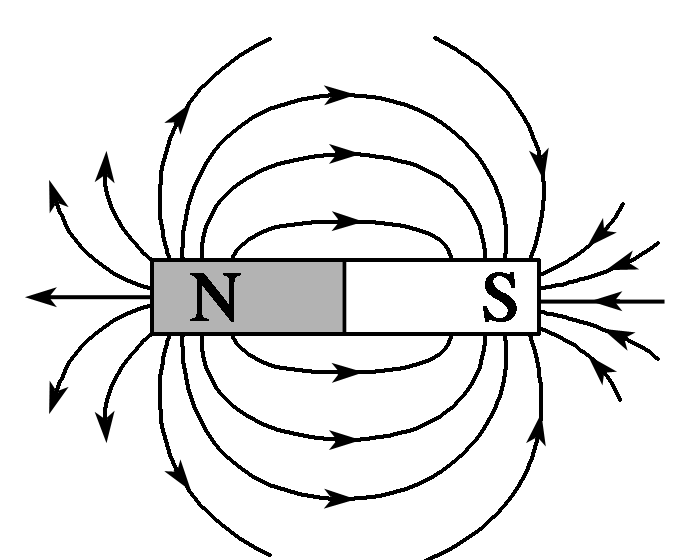
\includegraphics{./cichang/图片1.png}
  \qquad
  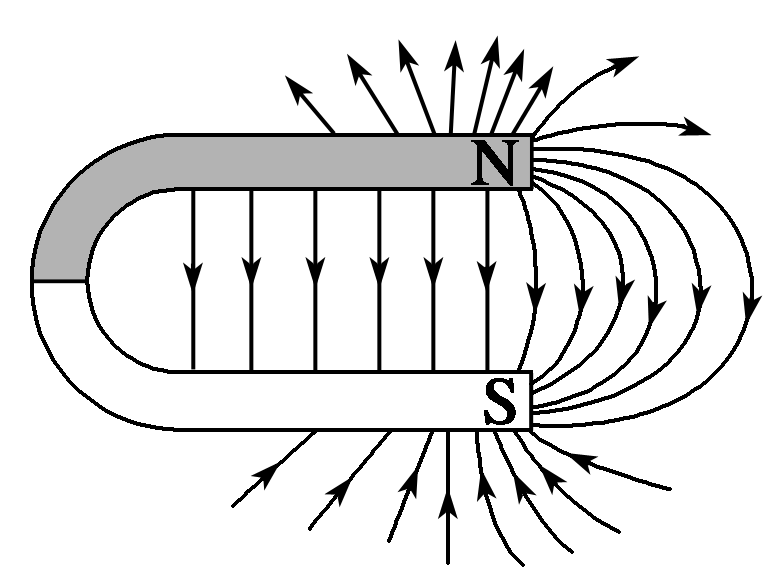
\includegraphics{./cichang/图片2.png}
  \caption{条形磁铁和蹄形磁铁}
\end{figure}
条形磁铁和蹄形磁铁是最常见的两类磁铁,其中蹄形磁铁两个磁极间的部分可以视为匀强磁场,即可以近似为等间距的平行线.这也是在以后各类计算题中经常出现的情况.


\begin{figure}[H]
  \centering
  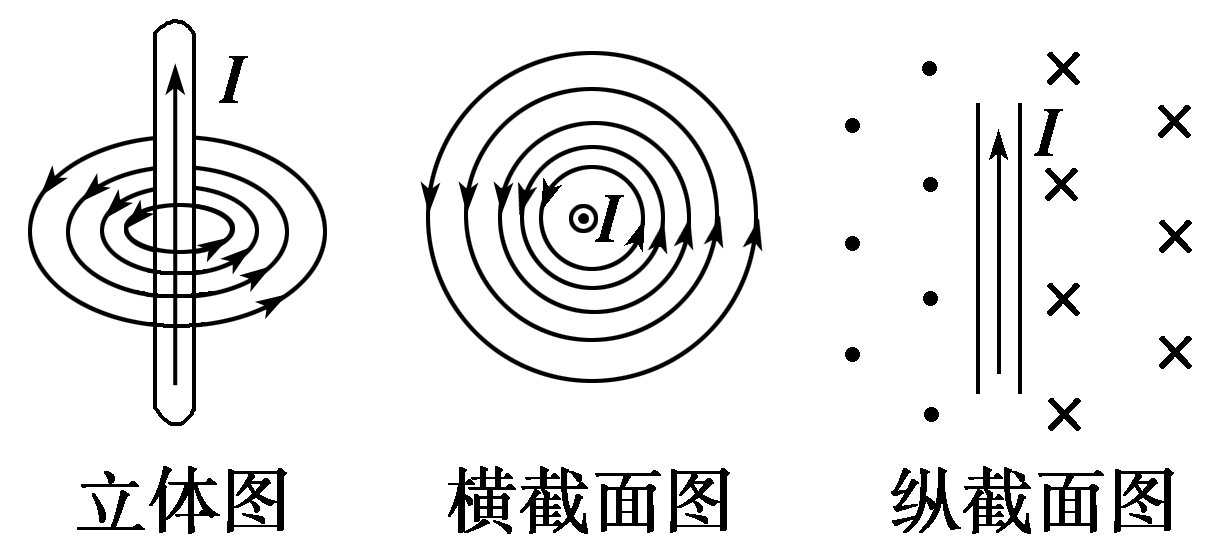
\includegraphics{./cichang/图片3.png}
  \caption{无限长直线电流的磁场}
\end{figure}
无限长直线电流的磁场:让右手握住导线,让伸直的拇指所指的方向与电流方向一致,弯曲的四指所指的方向就是\CJKunderwave{磁感线环绕的方向}. 这个规律也叫做右手定则.这里我们给大家指明一点,在以后我们还要计算安培力和洛仑兹力,它们的方向要用左手定则来判定,这时就有同学混淆了左手和右手的适用范围,我这样给大家解释:\CJKunderwave{在中国通常都是男左女右,而男生比较有力气,所以判定力的时候就是左手定则,其它的情况就是右手了.}这种磁场的特点是:以导线上各点为圆心的同心圆,圆所在的平面与导线{\bf 垂直},越向外{\bf 越疏}.

\begin{figure}[H]
  \centering
  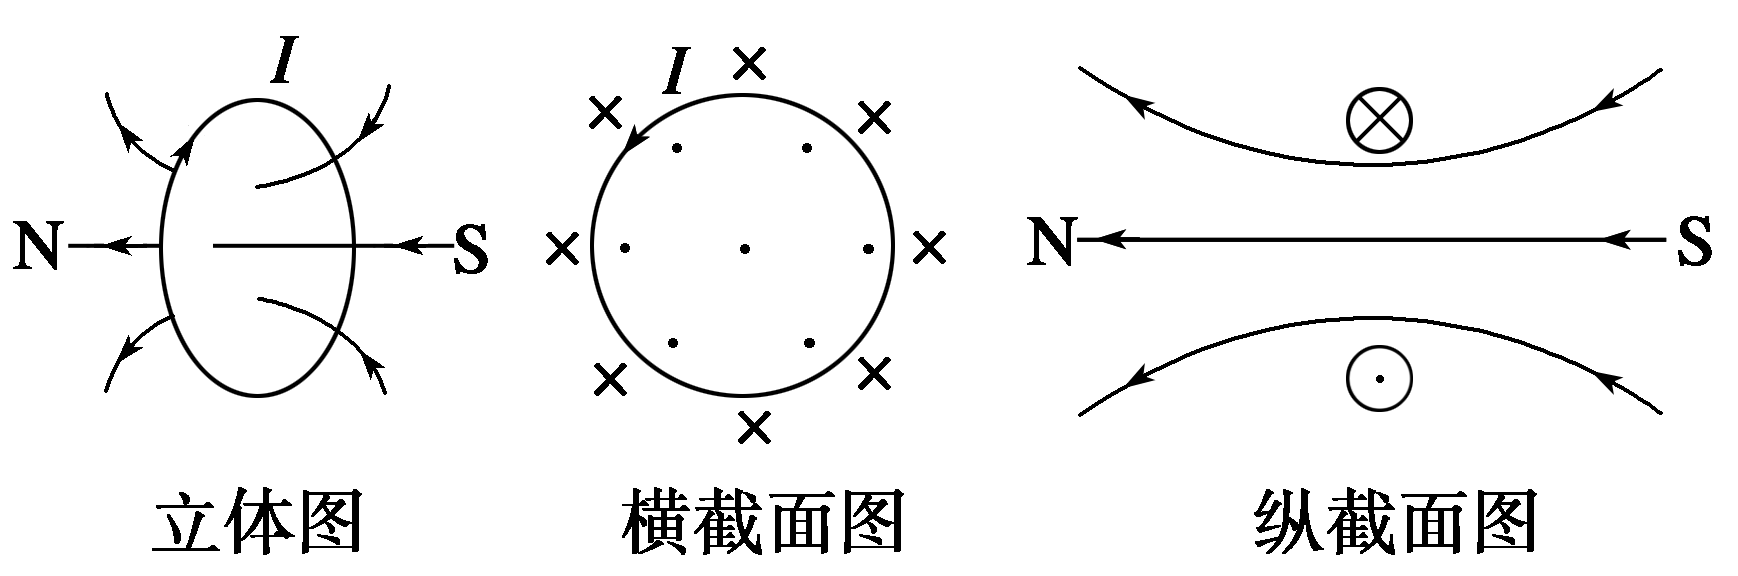
\includegraphics{./cichang/图片4.png}
  \caption{环形电流的磁场}
\end{figure}
环形电流的磁场:让右手弯曲的四指与\CJKunderwave{环形电流}的方向一致,伸直的拇指所指的方向就是\CJKunderwave{环形导线轴线}上磁感线的方向.其特点:内部比外部强,磁感线越向外越疏.

\begin{figure}[H]
  \centering
  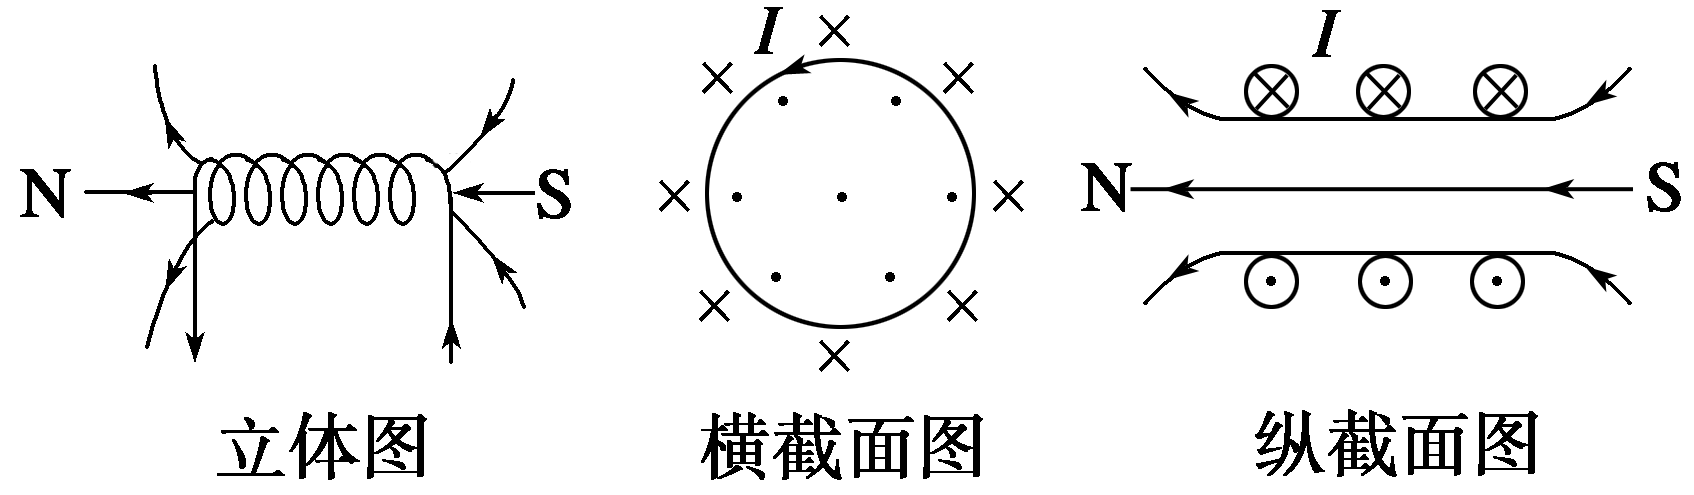
\includegraphics{./cichang/图片5.png}
  \caption{通电螺线管的磁场}
\end{figure}
通电螺线管的磁场:用右手握住螺线管,让弯曲的四指指向\CJKunderwave{电流}的方向,那么\CJKunderwave{大拇指}所指的方向就是螺线管中心轴线上磁感线的方向.其特点为:内部为\CJKunderwave{匀强磁场},且内部比外部强.内部磁感线方向由\CJKunderwave{S极}指向 \CJKunderwave{N极},外部由\CJKunderwave{N极}指向\CJKunderwave{S极}.

\subsection{安培分子电流假说}

安培分子电流假说认为:在原子,分子等物质微粒的内部,存在着一种环形电流------分子电流.分子电流相当于一个小磁针,它使每个物质微粒都成为微小的磁体,它的两侧相当于两个磁极.

\begin{figure}[H]
  \centering
  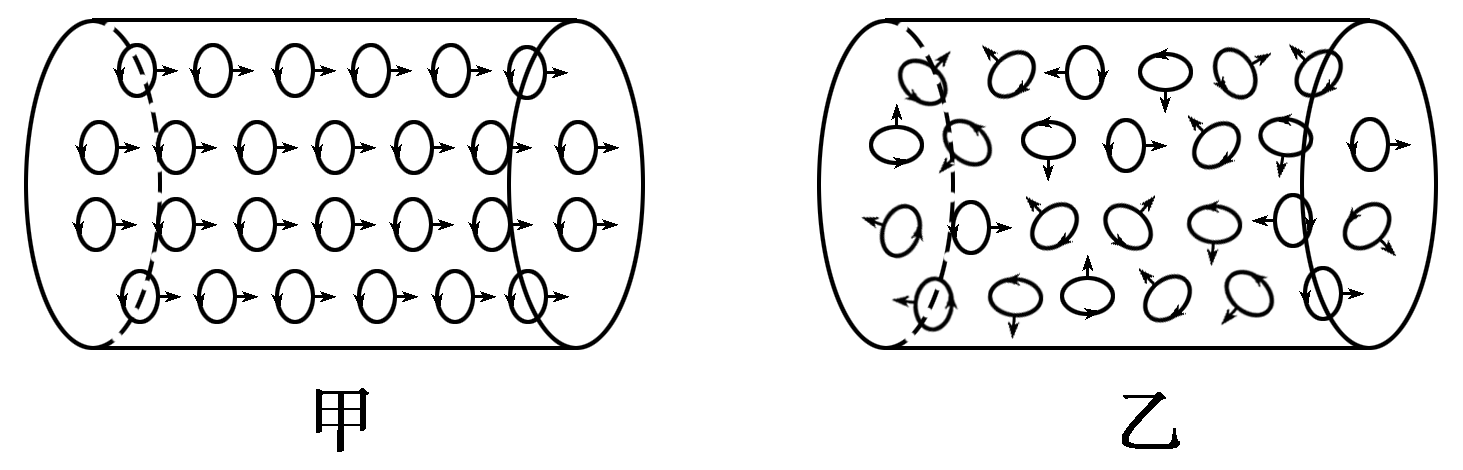
\includegraphics{./cichang/图片6.png}
  \caption{安培分子电流假说}
  \label{fig:anpeiI}
\end{figure}

如图\ref{fig:anpeiI}所示,当铁棒中分子电流的取向\CJKunderwave{大致相同}时,铁棒对外显磁性(如甲所示);当铁棒中分子电流的取向变得\CJKunderwave{杂乱无章}时,铁棒对外不显磁性(如图乙所示).安培分子电流假说说明\CJKunderwave{一切磁现象都是由电荷的运动产生的.}
\section{安培力}

当一段导线放入磁场中时会受到力,这个力叫做安培力.最简单的一种情况,是长直导线放入匀强磁场中,且满足导线与磁感应强度的方向相互垂直.如图\ref{fig:anpeiforce}所示,空间中充满垂直于纸面向里的匀强磁场,磁感应强度大小为$B$,在磁场中存在一根无限长直导线(无限长是相对于磁场来说的),导线的长度为$L$,导线中通有恒定电流,电流大小为$I$.

\begin{figure}[H]
  \centering
  \begin{tikzpicture}
    \foreach \x in {-1.4,-1,-0.6,-0.2,0.2,0.6,1,1.4} 
    \foreach \y in {-1.4,-1,-0.6,-0.2,0.2,0.6,1,1.4} 
    \draw (\x,\y) node {\small $\times$};
    \draw (-0.1,-1.2)--(-0.1,1.2);
    \draw (0.1,-1.2)--(0.1,1.2);
    \draw [->,>=stealth] (0,-0.5)--(0,0.5);
    \foreach \y in {-1.2,-0.9,-0.6,-0.3,0,0.3,0.6,0.9,1.2}
    \draw (-0.1,\y)--(0.1,\y);
    \foreach \y in {-1.2,-0.6,0,0.6,1.2}
    \draw[pattern=north west lines] (-0.1,\y) rectangle ++(0.2,0.3);
    \foreach \y in {-1.05,-0.75,-0.45,-0.15,0.15,0.45,0.75,1.05,1.35}
    \draw [->,>=stealth](0,\y)--++(-1,0) node [anchor=east] {\small $f$};
    \draw (0,-1.8) node [anchor=north] {\small 甲};
  \end{tikzpicture}
  \qquad
  \begin{tikzpicture}
    \foreach \x in {-1.4,-1,-0.6,-0.2,0.2,0.6,1,1.4} 
    \foreach \y in {-1.4,-1,-0.6,-0.2,0.2,0.6,1,1.4} 
    \draw (\x,\y) node {\small $\times$};
    \draw (-0.1,-1.2)--(-0.1,1.2);
    \draw (0.1,-1.2)--(0.1,1.2);
    \draw [->,>=stealth] (0,-0.5)--(0,0.5);
    \draw[->,>=stealth] (0,0)--++(-1.5,0) node [anchor=east]{\small $F$};
    \draw (0,-1.8) node [anchor=north] {\small 乙};
  \end{tikzpicture}
  \caption{安培力}
  \label{fig:anpeiforce}
\end{figure}

在图甲中, 我们可以将无限长直导线视为若干段相同的电流元,由于每一段电流元所处的环境是完全相同的,所以它们的受力情况也完全相同,即大小和方向都相同,按照磁感应强度$B$的定义,我们可以得到每一电流元的所力大小为$BI\Delta L$.然后我们将这无数个小电流元所受力叠加起来,则得到整个导线受到的力,由于匀强磁场和恒定电流,则$B$和$I$均是常量,则各力的方向又相同,所以叠加的结果就是各电流元的长度相加,而整体受力的方向与每一个小电流元受力方向相同,使用左手定则来判定即可.所心可得整个导线受到的力------安培力为
\begin{equation}
  F=BIL
  \label{eq:anpeiforce}
\end{equation}

\section{运动电荷在磁场中受到的力}

带电粒子在磁场中运动时相当于形成了电流,而电流在磁场中会受到力的作用,因此单个粒子在磁场中运动就会受到力的作用. 这一节我们的目标就是求出这个力的表达形式.考虑一个由全部相同的带电粒子所构成的电流元放入磁场中,由于是电流元所以其体积很小,其所处的磁场就可以视为匀强磁场,而电流元的电流恒定,由于所有带电粒子相同,所以在微观看来,每个带电粒子所处的环境是相同的,则每一个电荷所受到的力的大小和方向应当是一致的.因此,\CJKunderwave{电流元所受到力的方向就和单个电荷受力方向一致},这可以由左手定则来判定.其大小应当等于\CJKunderwave{电流元受力除以电流元中所含电荷的数目.}设电流元中电荷总数为$N$,电流元的长度为$\Delta L$,单位体积内电荷数目为$n$,每个电荷的带电量为$q$, 在所考虑的点上磁感应强度为$B$,则
\begin{gather}
 N=nS\Delta L 
 \label{eq:lorentz0}
 \intertext{由电流的微观定义式可得}
 I=nqvS
 \label{eq:lorentz1}
 \intertext{由式\eqref{eq:lorentz0}和式\eqref{eq:lorentz1}联立可以将电流元内的总电荷数用电流表达出来,为}
 N=\frac{I\Delta L}{qv}
 \label{eq:lorentz2}
 \intertext{电流元受力,由磁感应强度的定义可得为}
 F=BI\Delta L
 \label{eq:lorentz3}
 \intertext{由前述分析可得,每一个带电粒子所受力的大小为}
 f=\frac{F}{N}=qvB
 \intertext{所以我们就求出了一个带电粒子在磁场中所受到的力,这个力叫做洛仑兹力,重书如下}
 f=qvB
 \label{eq:lorentz4}
\end{gather}
{\bf 注意} 当我们判断洛仑兹力的方向时,使用左手定则,应当使磁感线由手掌穿入,手背穿出,四指指向\CJKunderwave{电荷所\CJKunderdot{形成电流}的方向},则拇指所指的方向就是洛仑兹力的方向.

我们注意,在上述讨论中我们使用的磁感应强度的定义来求出的电流元所受的力,仔细考虑这个问题,多少有些不严格,因为我们不能保证电流元放磁场时就一定与磁场垂直,此时我们再来讨论一下电流元与磁场不垂直的情况,如图\ref{fig:lorentz0}所示

\begin{figure}[H]
  \centering
  \begin{tikzpicture}
    \draw (-0.1,-1) rectangle (0.1,1);
    \draw[->,>=stealth] (0,-0.8)--(0,0.8);
    \draw [->,>=stealth] (0,0)--++(30:1) node [anchor=south west] {\small $B$};
    \draw [->,>=stealth] (0,0)--(0.866,0);
    \draw [->,>=stealth] (0,0)--(0,0.5);
    \draw[dashed](0,0)++(30:1)--++(0,-0.5) node [anchor=north] {\small $B\sin\theta$};
    \draw[dashed](0,0)++(30:1)--++(-0.866,0) node [anchor=east] {\small $B\cos\theta$};
    \draw (30:0.3) arc (30:90:0.3);
    \draw (60:0.45) node {\small $\theta$};
  \end{tikzpicture}
  \caption{电流元与磁场不垂直的情况}
  \label{fig:lorentz0}
\end{figure}

我们可以将磁感应强度$B$ 分解为与电流垂直的分量$B\sin\theta$ 和与电流平行的分量 $B\cos\theta$ ,但是平行分量对电流元无力的作用,只有垂直分量有力的作用,则此时电流元所受力的大小为
\begin{gather}
 F=I\Delta L\cdot B\sin\theta 
 \intertext{所以每个带电粒子在此时所受力的大小为}
 f=\frac{F}{N}
 \intertext{关于$N$的计算同前述一致,则洛仑兹力大小为}
 f=qvB\sin\theta 
 \label{eq:lorentz5}
\end{gather}
显然式\eqref{eq:lorentz5}是比\eqref{eq:lorentz4}更加普遍的表达式,如果令$\theta=\frac{\pi}{2}$,则就由式\eqref{eq:lorentz5}得到了式\eqref{eq:lorentz4}.

\section{带电粒子在匀强磁场中的运动}

上一节我们求出了洛仑兹力的表达式,确定了它的受力方向.如果带正电的粒子处于匀强磁场中,且速度方向与磁场垂直.则如图\ref{fig:lorentz1}所示

\begin{figure}[H]
  \centering
  \begin{tikzpicture}
    \foreach \x in {-1.4,-1,-0.6,-0.2,0.2,0.6,1,1.4} 
    \foreach \y in {-1.4,-1,-0.6,-0.2,0.2,0.6,1,1.4} 
    \draw (\x,\y) node {\small $\times$};
    \draw (0,0) circle [radius=1];
    \filldraw (0,1) circle [radius=1pt] node [anchor=south]{\small $q$};
    \draw[->,>=stealth] (0,1)--++(-0.8,0) node [anchor=south] {\small $v$};
    \draw[->,>=stealth] (0,1)--++(0,-0.8) node[anchor=west] {\small $f$};
    \draw[dashed](0,0)--++(90:1);
    \draw[dashed](0,0)--++(150:1);
    \filldraw (150:1) circle [radius=1pt] node [anchor=east] {\small $A$};
    \draw(90:0.3) arc (90:150:0.3);
    \draw(120:0.5) node {\small $\theta$};
  \end{tikzpicture}
  \caption{带电粒子在磁场中运动}
  \label{fig:lorentz1}
\end{figure}

由于洛仑兹力与速度每时每刻都垂直,所以我们可以得到结论:\CJKunderwave{洛仑兹力不做功}.在图\ref{fig:lorentz1}中速度与磁感应强度垂直,同时由左手定则可得,力也同时与速度和磁感应强度垂直,由于洛仑兹力不做功,显然带电粒子做\CJKunderwave{匀速直线运动}.我们的任务是计算出描述圆周运动的一些物理量.在圆周运动中起核心作用的就是角速度,所以我们先求解角速度,由牛顿第二定律得
\begin{gather}
 mv\omega=qvB 
 \intertext{解得}
 \omega=\frac{qB}{m}
\end{gather}
如图\ref{fig:lorentz1}中,带电粒子从开始的$q$ 位置运动到$A$位置 ,设其所用时间为$t$,则由圆周运动可得
\begin{gather}
  t=\frac{\theta}{\omega}\notag
  \intertext{代入角速度表达式可得}
  t=\frac{\theta m}{qB}
\end{gather}
 我们注意到,如果记转一周的时间为$T$,则它就是带电粒子做匀速圆周运动的周期,则
 \begin{gather}
   T=\frac{2\pi m}{qB}
 \end{gather}
 如果线速度$v$的大小已知,则由线速度与角速度的关系可得
\begin{gather}
  r=\frac{v}{\omega}\notag
  \intertext{代入角速度表达式得}
  r=\frac{mv}{qB}
\end{gather}

\subsubsection{质谱仪}

在自然界中有许多化学元素存在同位素,同位素的质子数相同,所以化学反应相同,但是它们的中子数不同,所以它们的物理反应是不同的.利用带电粒子在电磁场中做匀速圆周运动,可以区分同位素.如图\ref{fig:zhipuyi0}所示

\begin{figure}[H]
  \centering
  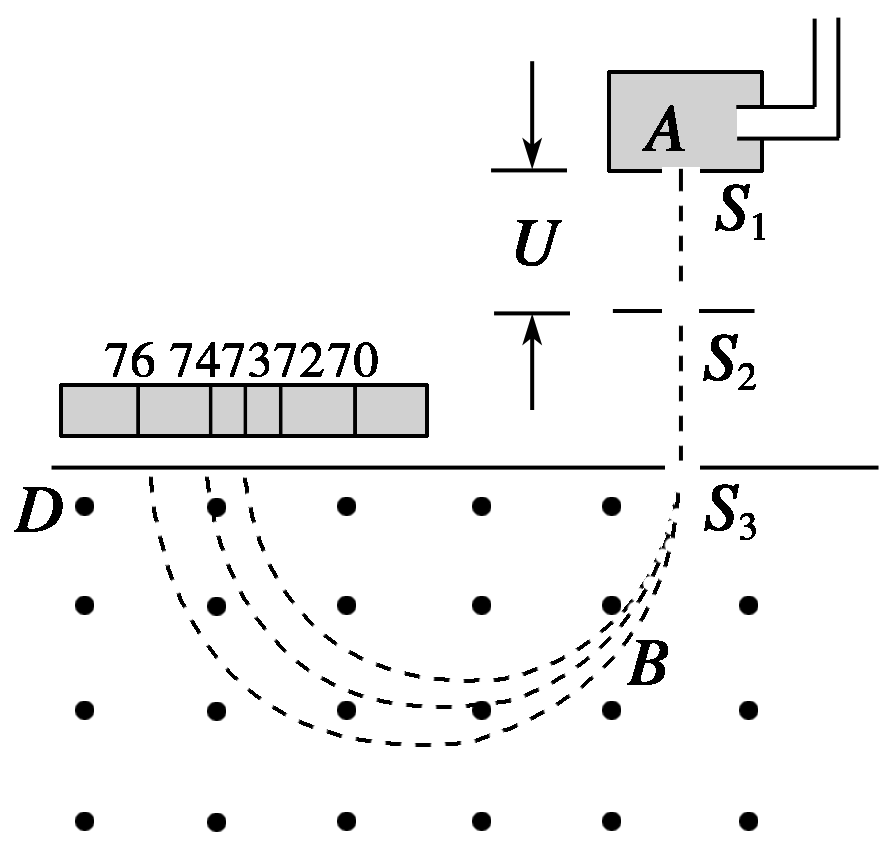
\includegraphics{./cichang/图片7.png}
  \caption{质谱仪}
  \label{fig:zhipuyi0}
\end{figure}

一个质量为$m$、电荷量为$q$的粒子,从容器$A$下方的小孔$S_1$飘入电势差为$U$ 的加速电场,其初速度几乎为$0$ ,然后经过$S_3$ 沿着与磁场垂直的方向进入磁感应为$B$ 的匀强磁场中,最后打到照相底片$D$上(图 \ref{fig:zhipuyi0}).求粒子在磁场中运动的轨道半径.

上面这道题是选自课本选修3---1 第100页 上的例题.为了求半径,我们根据带电粒子在磁场中运动时半径的表达式可知,首先我们需要求出速度$v$,根据动能定理可得
\begin{gather}
  qU=\frac{1}{2}mv^2-0
  \intertext{解得}
  v=\sqrt{\frac{2qU}{m}}
\end{gather}
由半径与线速度的关系可得
\begin{gather}
  r=\frac{mv}{qB}
  \intertext{将线速度代入上式得}
  r=\frac{m}{qB}\cdot\sqrt{\frac{2qU}{m}}
  \intertext{简单整理得}
  r=\frac{1}{B}\sqrt{\frac{2mU}{q}}
\end{gather}
由半径的表达式可得,只要带电粒子的比荷$\frac{q}{m}$ 相同,则粒子的轨迹半径就是相同的.比荷大的粒子,半径相应的小,从左侧底片上刻好刻度,则就能根据刻度来识别不同的同位素.

\subsubsection{回旋加速器}

在研究带电粒子的性质时,往往我们需要使用粒子相互撞击来了解一些粒子的信息.这就涉及到加速带电粒子的问题.通常需要粒子加速到很大的能量才能使粒子对撞而产生新的粒子等,根据动能定理,即
\begin{gather}
  qU=\frac{1}{2}mv^2
\end{gather}
我们可以通过电场加速粒子,而使其获得相应的动能.但是这里有一个问题就是,通常我们日常使用的电压是不会达到很高的,所以一次性加速粒子不能使其获得足够的能量.于是需要我们多次加速同一粒子.理论上我们可以使粒子通过多组平行板加速器,但是这在理论上可行,如果这样做的话,我们需要的设备过于庞大.但是我们注意到带电粒子在磁场中运动时其角速度($\omega=\frac{qB}{m}$)与线速度是无关的,进而粒子做匀速圆周运动的周期无论线速度多大都不发生变化.根据这一特殊的原理,美国著名物理学家 欧内斯$\cdot$劳伦斯(Ernest Orlando Lawrence)于1932年设计和制造了第一台高能粒子回旋加速器.如图\ref{fig:huixuanjiasu0}所示,是回旋加速器的原理图.

\begin{figure}[H]
  \centering
  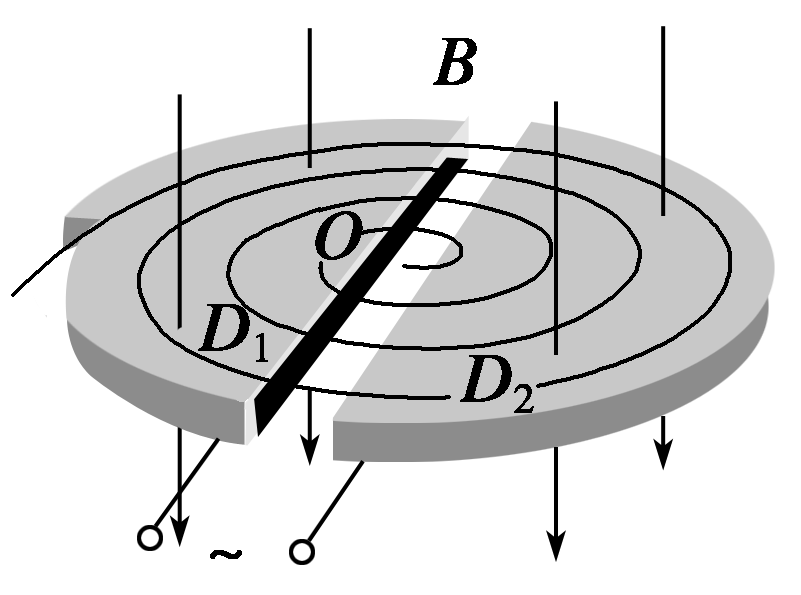
\includegraphics{./cichang/图片8.png}
  \caption{回旋加速器}
  \label{fig:huixuanjiasu0}
\end{figure}

回旋加速器由两个正对$D$ 型盒构成,在与两个$D$ 型盒正对的缝垂直的同时与$D$ 型盒的大表面平行的电场,由于静电屏蔽作用,则盒内部电场为零,但是接缝处电场不为零,并且两个$D$型盒是等势体,则接缝处的电势差在不同位置时都相同.在垂直于$D$ 型盒的方向,我们加上匀强磁场,金属盒不能屏蔽磁场,所以$D$型盒内部是存在匀强磁场的.所以带电粒子在$D$型盒内做匀速圆周运动,同时每半个周期粒子就穿过接缝,这里必须使电场与粒子的运动同步的改变正负极,这样粒子每次通过接缝就会加速一次.连续工作下去,带电粒子就能在$D$型盒内完成多次加速.最终的速度大小,取决于$D$型盒的半径,即
\begin{gather}
  v_m=R\frac{qB}{m} 
\end{gather}

但是大家注意,并不是此半径越大最终获得的速度越大.因为,当粒子加速到一定的程度后,它的速度若与光速可以比拟(即达到相同数量级),则按照相对论
\footnote{相对论是现今正确的力学理论,我们现在所学的力学实际上是速度远远小于光速的相对论近似,我们把现在大家学习的理论称为经典力学.我们不能说经典力学是错的,因为即便是用严格的相对论来处理问题,我们的公式最终也将近似到经典力学上来,而且作这个近似时,精确度还是相当相当高的.但是在物体高速运动时,经典力学就不适用了,而必须用相对论来解决.}
的理论粒子将会向外辐射电磁波,粒子将不会继续加速.所以现实中,回旋加速器确实实现了在小空间内加速粒子的目的.但是,一旦达到一定的速度它将不能再加速粒子,但是在回旋加速器后再追加若干组直线加速器,则粒子就可以继续加速.所以实现超高能的粒子,还需要直线加速器的.

为了清析的完成计算,我们画出俯视图如图\ref{fig:huixuanjiasu1}所示.我们知道,粒子每经过一次电场,则动能增加$qU$,带电粒子最初的速度接近为零,所以假设加速了$n$次,则最后的动能为$nqU$,所以可以求出加速$n$ 次的速度为
\begin{gather}
  nqU=\frac{1}{2}mv_n^2\notag
  \intertext{解得}
  v_n=\sqrt{\frac{2qU}{m}}\cdot \sqrt{n}
  \intertext{所以加速$n$次后的半径为}
  r_n=\frac{mv_n}{qB}=\frac{1}{B}\sqrt{2mU}{q}\cdot\sqrt{n}
  \intertext{所以各半径之比为}
  r_1:r_2:r_3:\cdots:r_n=\sqrt{1}:\sqrt{2}:\sqrt{3}:\cdots:\sqrt{n}
  \intertext{加速两次造成的半径变化为}
  \Delta r=r_1(\sqrt{n}-\sqrt{n-1})
\end{gather}
由此可得速度越大的时候半径差距越小.极限情况是最后的半径相同.这带来的好处是:轨道越来越密集,则可以将$D$形盒设计的更小一些.同时,最终的半径近似可以认为相同,而圆心近似在$D$形盒的中心.图\ref{fig:huixuanjiasu1}就是根据这个根号比严格画出来的图,我们设$D$型盒的半径为$R$,所以可以由此半径求出最大的速度$v_m$.

\begin{figure}[H]
  \centering
  \begin{tikzpicture}
    \foreach \x in {-0.1,0.1} 
    \draw (\x,-2)--(\x,2);
    \filldraw (-0.07,-0.5) circle [radius=1pt];
    \draw (-0.07,-0.5)--(0.1,-0.5);
    \draw [->,>=stealth] (0.1,-0.5)--++(0.5,0) node [anchor=north]{\small $v_1$};
    \draw (0.1,-0.5) arc (-90:90:0.5);
    \draw (0.1,0.5)--(-0.1,0.5);
    \draw (-0.1,0.5) arc (90:270:0.707);
    \draw (-0.1,-0.914)--(0.1,-0.914);
    \draw (0.1,-0.914) arc (-90:90:0.866);
    \draw (0.1,0.818)--(-0.1,0.818);
    \draw (-0.1,0.818) arc (90:270:1);
    \draw (-0.1,-1.182)--(0.1,-1.182);
    \draw(0.1,-1.182) arc (-90:90:1.118);
    \draw (0.1,1.054)--(-0.1,1.054);
    \draw (-0.1,1.054) arc (90:270:1.225);
    \draw (-0.1,-1.396)--(0.1,-1.396);
    \draw (0.1,-1.396) arc (-90:90:1.323);
    \draw (0.1,1.25)--(-0.1,1.25);
    \draw (-0.1,1.25) arc (90:270:1.414);
    \draw (-0.1,-1.578)--(0.1,-1.578);
    \draw (0.1,-1.578) arc (-90:90:1.5);
    \draw (0.1,1.422)--(-0.1,1.422);
    \draw (-0.1,1.422) arc (90:270:1.581);
    \draw (-0.1,-1.74)--(0.1,-1.74);
    \draw (0.1,-1.74) arc (-90:90:1.658);
    \draw (0.1,1.576)--(-0.1,1.576);
    \draw (-0.1,1.576) arc (90:270:1.732);
    \draw (-0.1,-1.888)--(0.1,-1.888);
    \draw (0.1,-1.888) arc (-90:90:1.803);
    \draw (0.1,1.718)--(-0.1,1.718);
    \filldraw (-0.1,1.718) circle [radius=1pt];
    \draw[->,>=stealth] (-0.1,1.718)--++(-1,0) node [anchor=south]{\small $v_{14}$};
    \foreach \x in {-2.2,-1.8,-1.4,-1,-0.6,-0.2,0.2,0.6,1,1.4,1.8,2.2}
    \foreach \y in {-2.2,-1.8,-1.4,-1,-0.6,-0.2,0.2,0.6,1,1.4,1.8,2.2}
    \draw (\x,\y) node {\small $\times$};
  \end{tikzpicture}
  \caption{回旋加速器俯视}
  \label{fig:huixuanjiasu1}
\end{figure}

下面我们来计算,粒子在回旋加速器中速度从$0$ 加速到最后所需要的时间.这个时间我们可以分两部分讨论,其一,粒子在磁场中的时间.其二,粒子在电场中的加速时间.在一般的讨论中由于接缝非常小,且粒子速度越来越大,但是在磁场中做匀速圆周运动的角速度是不变的,所以粒子加速的时间要远小于在磁场中匀速圆周运动的总时间.所以在近似度不是很高的计算中直接认为在磁场中运动的时间就是这个粒子在回旋加速器中的时间.此处,我们将严格来导出这两个时间.由最大速度$v_m$ ,我们可以求出最终的动能
\begin{gather}
  E_m=\frac{1}{2}mv_m^2=\frac{q^2B^2R^2}{2m}
  \intertext{粒子每次加速可以获得动能$qU$,所以总的加速次数$N$ 为}
  N=\frac{E_m}{qU}=\frac{qB^2R^2}{2mU}
  \intertext{由图\ref{fig:huixuanjiasu1}加速一次需要通过一次接缝和完成半个圆周运动,由于是匀速圆周运动,所以加速一次在磁场中用时半个周期$\frac{T}{2}$,我们先写出这个时间$t_1$,则}
  t_1=N\frac{T}{2}=\frac{qTB^2R^2}{4mU}
  \intertext{对于加速部分,由于我们所加电压大小保持不变,所以粒子在电场中做匀加速运动,而在磁场中仅起到一个转向 $180^\circ$ 的作用,所以整体上它和将粒子从 $0$ 直线以相同的加速度加速到 $v_m$ 所需时间是一致的.设接缝的宽度为 $d$,于是我们可以这样等效的求出这个时间$t_2$ }
  t_2=\frac{v_m}{a}=\frac{qBR}{m}\cdot \frac{md}{qU}=\frac{BRd}{U}
  \intertext{则总时间为这两个时间之和.即}
  t=t_1+t_2=\frac{qTB^2R^2}{4mU}+\frac{BRd}{U}
\end{gather}

\subsubsection{速度选择器}

由电场和磁场的配合,我们可以选择粒子的速度,这个设备叫做速度选择器.如图\ref{fig:suduxuanze0}所示,速度选择器由相互垂直的电场和磁场构成,其中磁场垂直于纸面向里,电场由上向下.对于图中所示一个带正电的粒子所受电场力向下,受洛仑兹力向上,如果二个力平衡,则粒子做匀速直线运动,最终通过右侧的出口$O$.如果电场力和洛仑兹力不等,则粒子将会发生偏转,而无法通过最右侧$O$.所以我们就实现的速度选择的目的.下面我们计算一下这个选择的速度,如下
\begin{gather}
 qvB-qE=0
 \intertext{解得}
 v=\frac{E}{B}
\end{gather}
大家注意,速度选择器与粒子的电性是无关的,因为若为负电,则电场力向上,洛仑兹力向下.由于保证平衡,则粒子必须是从左端射入,否则无法达到平衡,也就无法实现速度选择.

\begin{figure}[H]
  \centering
  \begin{tikzpicture}
    \draw (-2,-1.2) rectangle (2,-1); 
    \draw (-2,1.2) rectangle (2,1); 
    \filldraw (2,-1.2) rectangle (2.1,-0.05);
    \filldraw (2,1.2) rectangle (2.1,0.05);
    \foreach \x in {-1.8,-1.4,-1,-0.6,-0.2,0.2,0.6,1,1.4,1.8}
    \foreach \y in {-0.6,-0.2,0.2,0.6}
    \draw (\x,\y) node {\small $\times$};
    \foreach \x in {-1.8,-1.4,-1,-0.6,-0.2,0.2,0.6,1,1.4,1.8}
    \draw (\x,-1.1) node {\small $-$};
    \foreach \x in {-1.8,-1.4,-1,-0.6,-0.2,0.2,0.6,1,1.4,1.8}
    \draw (\x,1.1) node {\small $+$};
    \filldraw (-1.6,0) circle [radius=1pt] node [anchor=south east]{\small $q$};
    \draw[->,>=stealth] (-1.6,0)--++(1,0) node [anchor=west]{\small $v$};
    \draw[->,>=stealth] (-1.6,0)--++(0,0.5) node [anchor=west]{\small $qvB$};
    \draw[->,>=stealth] (-1.6,0)--++(0,-0.5) node [anchor=west]{\small $qE$};
    \draw (2,0) node [anchor=north west] {\small $O$};
  \end{tikzpicture}
  \caption{速度选择器}
  \label{fig:suduxuanze0}
\end{figure}

\subsubsection{霍尔元件}

利用带电粒子在磁场中的运动,我们还可以制成探测磁感应强度的仪器---霍尔元件.如图\ref{fig:huoer0}所示,在与恒定电流垂直的方向加以匀强电场$B$,与电流和磁感应强度$B$所在平面平行的两个表面记为$A$和$A'$,两个表面间距离为$h$, 沿磁场方向宽为$d$.

\begin{figure}[H]
  \centering
  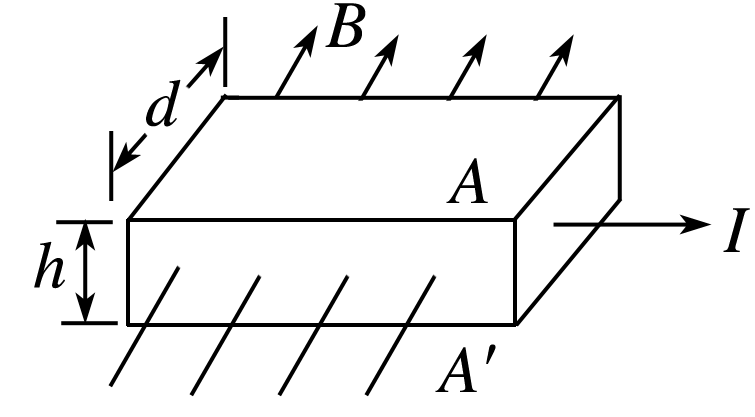
\includegraphics{./cichang/图片9.png}
  \caption{霍尔元件}
  \label{fig:huoer0}
\end{figure}

当所加磁场为$B$时,导体中的电荷将会受到洛仑兹力的作用.而向两个表面$A$ 和 $A'$ 偏转,进而形成与磁场和电流都垂直的电场.这就像速度选择器一样,所以当达到平衡时电荷将不再偏转,则$AA'$ 间的电势差将会磁感应强度$B$ 建立一一对应的关系.维持电流$I$不变,则测量$U_{AA'}$ 就能得到此时的磁感应强度$B$.电流的微观定义式为
\begin{gather}
  I=nqvS=nqvdh
  \intertext{解得电荷定向运动的速度$v$为}
  v=\frac{I}{nqdh}
  \intertext{由$AA'$方向受力平衡,可得}
  qvB-qE=0
  \intertext{解得电场强度$E$为}
  E=\frac{IB}{nqdh}
  \intertext{由匀强电场与电势差的关系可得横向电压$U_H$为}
  U_H=Eh=\frac{IB}{nqd}
  \intertext{记$k=\frac{1}{nq}$称为霍尔系数,则}
  U_H=k\frac{IB}{d}
\end{gather}
大家注意,对于不同的粒子,其所形成的电流都是图中所示方向,其不发生变化,所以参与导电的粒子所受洛仑兹力的方向也不发生变化,因此粒子的偏转方向也不发生变化.如正电荷定向移动,则其向$A$侧偏转,导到$U_{AA'}>0$,如负电荷,则也向$A$侧偏转,导致$U_{AA'}<0$,所以由横向电压与零的关系,我们就可以判断参与导电的电荷种类.
\subsubsection{磁流体发电机}

利用带电粒子在磁场中的运动时发生偏转还可以制成发电机---磁液体发电机.如图\ref{fig:ciliutifadian0}所示就是磁流体发电机的原理图.等离子体
\footnote{等离子体:物质是电中性的,当在处于高温时,分子会发生正负电荷的分离,所形成的物质整体电中性,但是由大量的正负离子构成,这种物质就叫做等离子体.}
从左侧射入,正离子所受洛仑兹力方向向上,负离子受洛仑兹力方向向下,因此上极板带正电,下极板带负电,所认在磁流体发电机中上下极板间会形成由上极板指向下极板的电场,因后来的正离子受电场力向下,受洛仑兹力方向向上,则在一段时间后必然会达到平衡.对于负离子,同理也可以达到平衡.当平衡时,离子不再发生偏转,而上下极板会维持一定的电势差,利用这个电势差就可以对外做功.故称磁流体发电机.

\begin{figure}[H]
  \centering
  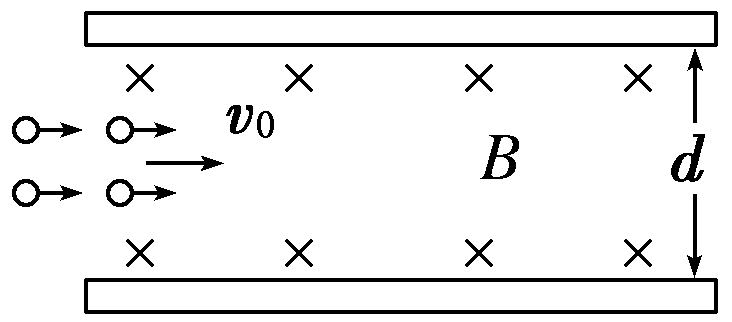
\includegraphics{./cichang/图片10.png}
  \caption{磁液体发电机}
  \label{fig:ciliutifadian0}
\end{figure}

当等离子体的射入速度恒定时,记为$v_0$, 两板间距离为$d$,所加匀强磁场为$B$,一个离子所带电为$q$,由当平衡时
\begin{gather}
  q\frac{U}{d}=qv_0B
  \intertext{解得}
  U=v_0Bd
\end{gather}

\subsubsection{电磁流量计}

利用带电粒子在磁场中的运动,我们还可以在不破坏管道的情况下进行流量的测定,这个仪器叫做电磁流量计.如图\ref{fig:dianciliuliangji0}所示,为电磁流量计的原理图.

\begin{figure}[H]
  \centering
  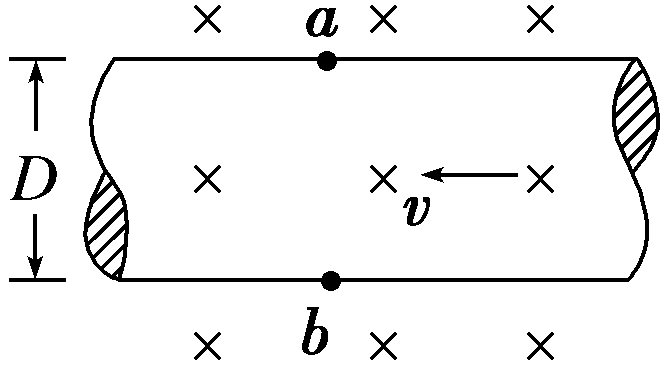
\includegraphics{./cichang/图片11.png}
  \caption{电磁流量计}
  \label{fig:dianciliuliangji0}
\end{figure}

我们先来介绍流量的概念.当液体流过一段管道时,我们可以用单位时间内流过横截面的体积来表示液体流动的快慢,这个物理量就是流量.设液体的速度为$v$,横截面积为$S$,流量为$Q$,则
\begin{gather}
  Q=vS
\end{gather}
如图\ref{fig:dianciliuliangji0}所示,管道的半径为$D$,同磁液体发电机一样,我们测得$ab$ 间的电压为$U$,高磁感应强度为$B$, 则
\begin{gather}
  E=\frac{U}{D}\notag\\
  v=\frac{E}{B}\notag\\
  v=\frac{U}{BD}\notag\\
  Q=vS=\frac{U}{BD}\frac{\pi D^2}{4}\notag
  \intertext{解得}
  Q=\frac{\pi DU}{4B}
\end{gather}
所以只要是测得了直径两端的电压$U$,我们就可以根据上述公式得到流量.电磁流量计可以使用的前提是流体内有带电离子,其优点是不用破坏管道的密闭性,比如在核电站中测量重水的流量,由于负责冷却反应堆的水是有辐射的,所以利用电磁流量计来测量流量会更加安全.

\subsubsection{功率仪}

此模型源自于2014年江苏高考题.如图\ref{fig:gonglvyi}所示,导电物质为电子的的霍尔元件位于两串联线圈之间,线圈中电流为$I$,线圈间产生匀强磁场,磁感应强度大小$B$ 与电流$I$ 成正比,方向垂直于霍尔元件的两个侧面,此时霍尔元件的电流为$I_H$, 与其前后表面相边的电压表测出的霍尔电压$U_H$ 满足:$U_H=k\frac{I_HB}{d}$,式中$k$ 为霍尔系数,$d$为霍尔元件两侧面间的距离.电阻$R$ 远大于$R_L$,霍尔元件的电阻可以忽略,则\CJKunderwave{电压表的示数与\mbox{$R_L$}消耗的电功率成正比}.

\begin{figure}[H]
  \centering
  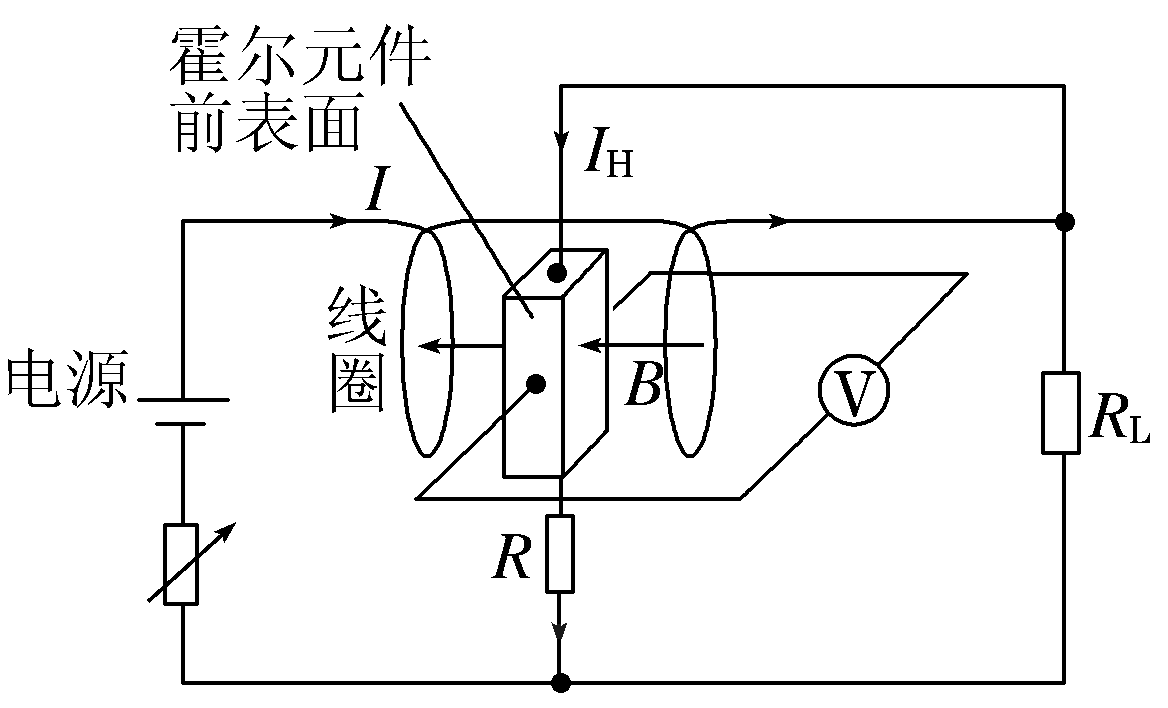
\includegraphics{./cichang/图片13.png}
  \caption{功率仪}
  \label{fig:gonglvyi}
\end{figure}

由于磁感应强度$B$与电流$I$成正比,而电阻$R$和$R_L$ 又是并联,则有
\begin{gather}
  I_H R=(I-I_H)R_L
  \intertext{解得}
  \frac{I_H}{I}=\frac{R_L}{R+R_L}
  \intertext{上式表明$I_H$ 和 $I$ 成正比,同时$I$与$B$成正比,所以$I_H$ 与$B$ 成正比.而霍尔电压为}
  U_H=k\frac{I_HB}{d}
  \intertext{由于$B$ 和$I_H$ 成正比,所以有}
  U_H \propto I_H^2 \propto I^2
  \intertext{由于$R_L$ 上的功率为$P=I^2R_L$,所以可得}
  U_H \propto P
\end{gather}

\chapter{高中数学若干问题}
这一章主要记录本人在读高中的时候处理一些典型数学问题的方法,用以提高大家的数学计算能力.同时也为了表明一个物理老师的是如何处理数学问题的,相信同学们在仔细钻研后肯定有所收获.
\section{对称点问题和点到直线的距离}
记直线L的某一由$(x_2,y_2)$指向$(x_1,y_1)$的法向量$\vec{n}$,则$\vec{n}$与$(x_1-x_2,y_1-y_2)$平行.$(x_0,y_0)$为L上任意一点,则$(x_1-x_0,y_1-y_0)\cdot \vec{n}$为$(x_1,y_1)$到L的距离.如图\ref{fig:duichengdian}所示
\begin{figure}[H]
  \centering
  \begin{tikzpicture}
    \draw[->,>=stealth](-3,0)--(3,0) node [anchor=north]{\small x};
    \draw[->,>=stealth](0,-3)--(0,3) node [anchor=west]{\small y};
    \draw (-1,-2)--(3,2);
    \filldraw(0.5,-0.5) circle [radius=1pt] node [anchor=south east] {\tiny $(x_0,y_0)$};
    \filldraw(0.5,1) circle [radius=1pt] node [anchor=south east]{\tiny $(x_1,y_1)$};
    \filldraw(2,-0.5) circle [radius=1pt] node [anchor=north west]{\tiny $(x_2,y_2)$};
    \draw [->,>=stealth](0.5,-0.5)--(0.5,1);
    \draw [->,>=stealth](2,-0.5)--(0.5,1);
  \end{tikzpicture}
  \caption{对称点问题}
  \label{fig:duichengdian}
\end{figure}

\begin{gather}
  \intertext{下面再来研究$(x_1,y_1)$与$(x_2,y_2)$关于L对称.则$(x_1-x_2,y_1-y_2)$的模是$(x_1,y_1)$到L距离的$2$倍,则}
  (x_1-x_2,y_1-y_2)=2(x_1-x_0,y_1-y_0)\cdot \vec{n}\vec{n}
  \intertext{看上式的右式,如将$\vec{n'}=-\vec{n}$作替换,则有}
  (x_1-x_2,y_1-y_2)=2(x_1-x_0,y_1-y_0)\cdot \vec{n}\vec{n}=2(x_1-x_0,y_1-y_0)\cdot\vec{n'}\vec{n'}
  \intertext{上式表明无论是$\vec{n}$还是$\vec{n'}$,不需要考虑其方向由$(x_1,y1)$指向$(x_2,y_2)$还是由$(x_2,y_2)$指向$(x_1,y_1)$则等式永远成立.于是可以取L的一个法向量为}
  \vec{n}=\frac{(A,B)}{\sqrt{A^2+B^2}}
  \intertext{则有}
  (x_1-x_2,y_1-y_2)=2(x_1-x_0,y_1-y_0)\cdot\frac{(A,B)}{\sqrt{A^2+B^2}}\frac{(A,B)}{\sqrt{A^2+B^2}}\\
  (x_1-x_2,y_1-y_2)=2\frac{Ax_1+By_1+C}{A^2+B^2}(A,B)
  \intertext{解得}
  x_2=x_1-\frac{2A}{A^2+B^2}(Ax_1+Bx_1+C)\\
  y_2=y_1-\frac{2B}{A^2+B^2}(Ax_1+Bx_1+C)
  \intertext{若$(x_1,y_1)$为已知点,则由此公式可以方便的求出对称点.同时可以求出点到直线的距离$d$为}
d=|(x_1-x_0,y_1-y_0)\cdot\vec{n}|
\intertext{即}
d=\frac{|Ax_1+By_1+C|}{\sqrt{A^2+B^2}}
\intertext{注意:上式中由于$(x_0,y_0)$在L上,则$Ax_0+B_0+C=0$于是有$C=-Ax_0-By_0$.}\notag
\end{gather}
\section{立体几何的二面角的求解}
\subsection{三角公式法}
如图所示,记平面$\Sigma$和平面$\Sigma$二面角为$\gamma$则
\begin{figure}[H]
  \centering
  \begin{tikzpicture}
    \draw(0,0)--(0:2)--++(20:2.5)--++(180:2);
    \draw(0,0)--(20:2.5);
    \draw(0,0)--(60:1.5)--++(20:2.5)--++(240:1.5);
    \draw[->,>=stealth](0,0)--(0:1);
    \draw[->,>=stealth](0,0)--(20:0.6);
    \draw[->,>=stealth](0,0)--(60:1);
    \draw (0:0.4) arc (0:60:0.4);
    \draw (0:0.6) arc (0:20:0.6);
    \draw (20:0.5) arc (20:60:0.5);
    \draw (35:0.2) node {\tiny $\theta$};
    \draw (10:0.7) node {\tiny $\alpha$};
    \draw (40:0.7) node {\tiny $\beta$};
    \draw (10:2) node {\tiny $\Sigma'$};
    \draw (40:2) node {\tiny $\Sigma$};
  \end{tikzpicture}
  \caption{三角公式法}
  \label{fig:ermianjiao1}
\end{figure}
\begin{gather}
  (\vec{n_2}-\vec{n_2}\cdot\vec{n}\vec{n})\cdot(\vec{n_1}-\vec{n_1}\cdot\vec{n}\vec{n})=\sin\alpha\sin\beta\cos\gamma\\
  \vec{n_2}\cdot\vec{n_1}-\vec{n_1}\cdot\vec{n}\vec{n_2}\cdot\vec{n}-\vec{n_2}\cdot\vec{n}\vec{n_1}\cdot\vec{n}+\vec{n_1}\cdot\vec{n}\vec{n_2}\cdot\vec{n}=\sin\alpha\sin\beta\cos\gamma\\
  \cos\theta-\cos\alpha\cos\beta=\sin\alpha\sin\beta\cdot\cos\gamma\\
  \cos\gamma=\frac{\cos\theta-\cos\alpha\cos\beta}{\sin\alpha\sin\beta}
  \intertext{知道角$\alpha,\beta,\theta$可直接算出$\gamma$的余弦值.}\notag
\end{gather}
\subsection{采用内积的坐标算法}
如图\ref{fig:ermianjiao2}所示,遇到立体几何问题要毫不犹豫的写出以下 o,A,B,C几个点的坐标,其中$OB$为平面$\Sigma$和平面$\Sigma'$的交线.作$CC'\bot OB$于$C'$,$A'A\bot OB$于$A'$.
\begin{gather}
  \intertext{类比上一节的计算可得}
  \overset{\longrightarrow}{C'C}=\overset{\longrightarrow}{OC}-\frac{\overset{\longrightarrow}{OC}\cdot \overset{\longrightarrow}{OB}}{|\overset{\longrightarrow}{OB}|^2}\overset{\longrightarrow}{OB}
  \intertext{同理}
  \overset{\longrightarrow}{A'A}=\overset{\longrightarrow}{OA}-\frac{\overset{\longrightarrow}{OA}\cdot \overset{\longrightarrow}{OB}}{|\overset{\longrightarrow}{OB}|^2}\overset{\longrightarrow}{OB}
  \intertext{于是$\Sigma$和$\Sigma'$的夹角$\gamma$为}
  \cos\gamma=\frac{\overset{\longrightarrow}{C'C}\cdot\overset{\longrightarrow}{A'A}}{|\overset{\longrightarrow}{C'C}|\cdot|\overset{\longrightarrow}{A'A}|}
  \intertext{注意:所有这些都要用坐标运算,不需要多做考虑,对于应对高考的数学解析几何是一个相当大的优势.}\notag
\end{gather}
\begin{figure}[H]
  \centering
  \begin{tikzpicture}
    \draw(0,0)--(0:2)--++(20:2.5)--++(180:2);
    \draw[->,>=stealth](0,0)--(20:2.5) node [anchor=south west]{\tiny $B$};
    \draw(0,0)--(60:1.5)--++(20:2.5)--++(240:1.5);
    \draw[->,>=stealth](0,0)--(0:2) node [anchor=north west]{\tiny $A$};
    \draw[->,>=stealth](0,0)--(20:0.6) node [anchor=east]{\tiny $C'$};
    \draw[->,>=stealth](0,0)--(60:1.5) node [anchor=south east]{\tiny $C$};
    \draw(0,0) node [anchor=north east]{\tiny O};
    \draw[->,>=stealth](20:0.6)--(60:1.5);
    \draw[->,>=stealth](0,0)--(20:0.8) node [anchor=west]{\tiny $A'$};
    \draw[->,>=stealth](20:0.8)--(0:2);
    \draw (10:2) node {\tiny $\Sigma'$};
    \draw (40:2) node {\tiny $\Sigma$};
  \end{tikzpicture}
  \caption{坐标算法}
  \label{fig:ermianjiao2}
\end{figure}
\subsection{采用外积的坐标算法}
外积的定义为:
\begin{equation}
  \vec{a}\times\vec{b}=ab\sin\theta \vec{n}
\end{equation}
\begin{figure}[H]
  \centering
  \begin{tikzpicture}
  \draw[->,>=stealth](0,0)--(0:2) node [anchor=west]{\tiny $\vec{a}$};
  \draw[->,>=stealth](0,0)--(20:2) node [anchor=south]{\tiny $\vec{b}$};
  \draw[->,>=stealth](0,0)--(90:1) node [anchor=east]{\tiny $\vec{n}$};
  \draw[->,>=stealth](0:1) arc (0:20:1);
  \draw[pattern=north west lines](0,0)--++(0:2)--++(20:2)--++(180:2)--++(200:2);
  \draw (8:1.3) node {\tiny $\theta$};
  \end{tikzpicture}
  \caption{外积的方向}
  \label{fig:waiji}
\end{figure}
其中$\vec{n}$垂直于$\vec{a}$和$\vec{b}$所在平面,外积是一个矢量,它的大小为图\ref{fig:waiji}所示的阴影的面积,方向就是$\vec{n}$的方向.

\subsection{矢量外积的坐标式}
\begin{gather}
\intertext{记$\vec{a}=(a_1,a_2,a_3)$,$\vec{b}=(b_1,b_2,b_3)$则}
\vec{a}\times\vec{b}=
\begin{vmatrix}
  \vec{i}&\vec{j}&\vec{k}\\
  a_1&a_2&a_3\\
  b_1&b_2&b_3
\end{vmatrix}
=
\begin{vmatrix}
  a_2&a_3\\
  b_2&b_3
\end{vmatrix}\vec{i}
-
\begin{vmatrix}
  a_1&a_3\\
  b_1&b_3
\end{vmatrix}\vec{j}
+
\begin{vmatrix}
  a_1&a_2\\
  b_1&b_2
\end{vmatrix}\vec{k}
\intertext{例:外积的计算,如果$\vec{a}=(1,1,2),\vec{b}=(1,0,3)$则}
\vec{a}\times\vec{b}=
\begin{vmatrix}
  \vec{i}&\vec{j}&\vec{k}\\
  1&1&2\\
  1&0&3
\end{vmatrix}
=
\begin{vmatrix}
  1&2\\
  0&3
\end{vmatrix}\vec{i}
-
\begin{vmatrix}
  1&2\\
  1&3
\end{vmatrix}\vec{j}
+
\begin{vmatrix}
  1&1\\
  1&0
\end{vmatrix}\vec{k}\\
\vec{a}\times\vec{b}=3\vec{i}-\vec{j}-\vec{k}=(3,-1,-1)
\end{gather}

如图\ref{fig:waiji2}所示
\begin{figure}[H]
  \centering
  \begin{tikzpicture}
    \draw(0,0)--(0:2)--++(20:2.5)--++(180:2);
    \draw[->,>=stealth](0,0)--(20:2.5) node [anchor=south west]{\tiny $B$};
    \draw(0,0)--(60:1.5)--++(20:2.5)--++(240:1.5);
    \draw[->,>=stealth](0,0)--(0:2) node [anchor=north west]{\tiny $A$};
    \draw[->,>=stealth](0,0)--(60:1.5) node [anchor=south east]{\tiny $C$};
    \draw(0,0) node [anchor=north east]{\tiny O};
    \draw (10:2) node {\tiny $\Sigma$};
    \draw (40:2) node {\tiny $\Sigma'$};
    \draw [->,>=stealth] (0:1) arc (0:20:1);
    \draw [->,>=stealth] (0:1.5)--++(90:1) node [anchor=west]{\tiny $\vec{n}$};
    \draw [->,>=stealth] (60:1)--++(150:1) node [anchor=west]{\tiny $\vec{n'}$};
  \end{tikzpicture}
  \caption{外积计算二面角}
  \label{fig:waiji2}
\end{figure}

\begin{gather}
  \intertext{$\overset{\longrightarrow}{OA}$和$\overset{\longrightarrow}{OB}$,$\overset{\longrightarrow}{OC}$均可以用坐标方便的表示出来,无需考虑具体的几何关系,则}
  \vec{n}=\overset{\longrightarrow}{OA}\times\overset{\longrightarrow}{OB}\\
  \vec{n}=\overset{\longrightarrow}{OC}\times\overset{\longrightarrow}{OB}
  \intertext{则$\Sigma'$和$\Sigma$的夹角$\gamma$可以由它们的法向量$\vec{n}$和$\vec{n'}$示得,如下}
  \cos\gamma=\frac{\vec{n'}\cdot\vec{n}}{|\vec{n'}|\cdot|\vec{n}|}
  \intertext{注意:在所介绍的这三种方法中,外积法高中数学没有介绍,但是此法最简单,练熟后大题采用上式,则不用寻找具体的几何关系,可以直接写出答案.}\notag
\end{gather}
\section{三角函数变换公式}
关于三角函数问题要学会和、差、倍、半、万能公式的推理论证,否则此类问题将会消耗更多的时间.下面我详证这些关系.
首先由余弦定理导出差角公式,关于余弦公式前面在力的合成分解中已经详细论证了,这里不再赘述.如图\ref{fig:chajiao}所示
\begin{figure}[H]
  \centering
  \begin{tikzpicture}
    \draw[->,>=stealth] (-2,0)--(2,0); 
    \draw[->,>=stealth] (0,-2)--(0,2); 
    \draw (0,0) circle [radius=1];
    \draw (0,0)--(30:1) node [anchor=west]{\tiny $A$};
    \draw (0,0)--(120:1) node [anchor=east]{\tiny $B$};
    \draw(30:1)--(120:1);
    \draw (0:0.5) arc (0:30:0.5);
    \draw (0:0.3) arc (0:120:0.3);
    \draw (15:0.6) node {\tiny $\beta$};
    \draw (60:0.4) node {\tiny $\alpha$};
  \end{tikzpicture}
  \caption{差角公式}
  \label{fig:chajiao}
\end{figure}
\begin{gather}
  \intertext{由图\ref{fig:chajiao}可知$A(\cos\beta,\sin\beta)$,$B(\cos\alpha,\sin\alpha)$,再由余弦定理可得}
  (\cos\alpha-\cos\beta)^2+(\sin\alpha-\sin\beta)^2=1+1-2\cos(\alpha-\beta)\notag\\
  \cos(\alpha-\beta)=\cos\alpha\cos\beta+\sin\alpha\sin\beta
  \label{eq:chajiao0}
  \intertext{上式中取$\beta$替换为$-\beta$得}
  \cos(\alpha+\beta)=\cos\alpha\cos\beta-\sin\alpha\sin\beta
  \label{eq:chajiao1}
  \intertext{对式\eqref{eq:chajiao1}将$\alpha$视为变量$\beta$视为常量,对$\alpha$求导则}
  -\sin(\alpha+\beta)=-\sin\alpha\cos\beta-\cos\alpha\sin\beta\notag\\
  \sin(\alpha+\beta)=\sin\alpha\cos\beta\cos\alpha\sin\beta
  \intertext{同理对式\eqref{eq:chajiao0}将$\alpha$视为变量$\beta$视为常量,对$\alpha$求导得}
  -\sin(\alpha-\beta)=-\sin\alpha\cos\beta+\cos\alpha\sin\beta\notag\\
  \sin(\alpha-\beta)=\sin\alpha\cos\beta-\cos\alpha\sin\beta
  \intertext{综上所述,得{\bf 和角公式}为}
  \left\{
    \begin{gathered}
      \sin(\alpha+\beta)=\sin\alpha\cos\beta+\cos\alpha\sin\beta\\
      \cos(\alpha+\beta)=\cos\alpha\cos\beta-\sin\alpha\sin\beta
    \end{gathered}
  \right.
  \label{eq:hejiao}
  \intertext{{\bf 差角公式}为}
  \left\{
    \begin{gathered}
      \sin(\alpha-\beta)=\sin\alpha\cos\beta-\cos\alpha\sin\beta\\
      \cos(\alpha-\beta)=\cos\alpha\cos\beta+\sin\alpha\sin\beta
    \end{gathered}
  \right.
  \label{eq:chajiao}
  \intertext{取$\alpha=\beta$代入和角公式\eqref{eq:hejiao}得{\bf 倍角公式}}
  \left\{
    \begin{gathered}
      \sin2\alpha=2\sin\alpha\cos\alpha\\
      \cos2\alpha=\cos^2\alpha-\sin^2\alpha
    \end{gathered}
  \right.
  \label{eq:beijiao}
  \intertext{考虑到$\sin^2\alpha+\cos^2\alpha=1$得}
  \cos2\alpha=1-2\sin^2\alpha\notag\\
  \label{eq:beijiao0}
  \sin\alpha=\pm\sqrt{\frac{1-\cos2\alpha}{2}}
  \intertext{上式中$\pm$取决于$\alpha$的象限,取$\frac{\alpha}{2}$代换$\alpha$得}
  \sin\frac{\alpha}{2}=\pm\sqrt{\frac{1-\cos\alpha}{2}}
  \intertext{同理由\eqref{eq:beijiao}可得}
  \cos2\alpha=2\cos^2\alpha-1\notag\\
  \cos\alpha=\pm\sqrt{\frac{1+\cos2\alpha}{2}}
  \intertext{同理令$\frac{\alpha}{2}$取代$\alpha$得}
  \cos\frac{\alpha}{2}=\pm\sqrt{\frac{1+\cos\alpha}{2}}
  \intertext{写到一块得{\bf 半角公式}}
  \left\{
    \begin{gathered}
      \sin\frac{\alpha}{2}=\pm\sqrt{\frac{1-\cos\alpha}{2}}\\
      \cos\frac{\alpha}{2}=\pm\sqrt{\frac{1+\cos\alpha}{2}}
    \end{gathered}
    \right.
    \intertext{下面论证万能公式}
    \tan(\alpha+\beta)=\frac{\sin(\alpha+\beta)}{\cos(\alpha+\beta)}=\frac{\sin\alpha\cos\beta+\cos\alpha\sin\beta}{\cos\alpha\cos\beta-\sin\alpha\sin\beta}
    \intertext{上式分子分母同时除以$\cos\alpha\cos\beta$得{\bf 万能公式第一式}}
    \tan(\alpha+\beta)=\frac{\tan\alpha+\tan\beta}{1-\tan\alpha\tan\beta}
    \label{eq:wanneng0}
    \intertext{上式\eqref{eq:wanneng0}中令$\beta$替换为$-\beta$则}
    \tan(\alpha-\beta)=\frac{\tan\alpha-\tan\beta}{1+\tan\alpha\tan\beta}
    \label{eq:wanneng1}
    \intertext{式\eqref{eq:wanneng0}中令$\alpha=\beta$则}
    \tan2\alpha=\frac{2\tan\alpha}{1-\tan^2\alpha}
    \intertext{上式中令$\alpha$代换为$\frac{\alpha}{2}$}
    \tan\alpha=\frac{2\tan\frac{\alpha}{2}}{1-\tan^2\frac{\alpha}{2}}
    \intertext{同时}
    \sin\alpha=2\sin\frac{\alpha}{2}\cos\frac{\alpha}{2}=\frac{2\sin\frac{\alpha}{2}\cos\frac{\alpha}{2}}{\sin^2\frac{\alpha}{2}+\cos^2\frac{\alpha}{2}}=\frac{2\tan\frac{\alpha}{2}}{1+\tan^2\frac{\alpha}{2}}\\
    \cos\alpha=\frac{\sin\alpha}{\tan\alpha}=\frac{1-\tan^2\frac{\alpha}{2}}{1+\tan^2\frac{\alpha}{2}}
    \intertext{通过上面的论证,我们把$\tan\alpha,\sin\alpha,\cos\alpha$都表达成了$\tan\frac{\alpha}{2}$的函数,所以原则上所有的三角函数都可以表达成$\tan\frac{\alpha}{2}$的函数,基于这个原因我们把下面这组式称为{\bf 万能公式}}
    \begin{gathered}
      \tan\alpha=\frac{2\tan\frac{\alpha}{2}}{1-\tan^2\frac{\alpha}{2}}\\
      \sin\alpha=\frac{2\tan\frac{\alpha}{2}}{1+\tan^2\frac{\alpha}{2}}\\
      \cos\alpha=\frac{1-\tan^2\frac{\alpha}{2}}{1+\tan^2\frac{\alpha}{2}}
    \end{gathered}
    \intertext{这几个公式在不定积分中有重要的应用,所以也是必须掌握的.为了清析起见,这里分组列出这几个重要的公式.}\notag
  \end{gather}
  \begin{gather}
    \intertext{{\bf 和角公式:}}
  \left\{
    \begin{gathered}
      \sin(\alpha+\beta)=\sin\alpha\cos\beta+\cos\alpha\sin\beta\\
      \cos(\alpha+\beta)=\cos\alpha\cos\beta-\sin\alpha\sin\beta\\
      \tan(\alpha+\beta)=\frac{\tan\alpha+\tan\beta}{1-\tan\alpha\tan\beta}
    \end{gathered}
  \right.\\
  \intertext{{\bf 差角公式:}}
  \left\{
    \begin{gathered}
      \sin(\alpha-\beta)=\sin\alpha\cos\beta-\cos\alpha\sin\beta\\
      \cos(\alpha-\beta)=\cos\alpha\cos\beta+\sin\alpha\sin\beta\\
      \tan(\alpha-\beta)=\frac{\tan\alpha-\tan\beta}{1+\tan\alpha\tan\beta}
    \end{gathered}
  \right.\\
  \intertext{{\bf 倍角公式:}}
  \left\{
    \begin{gathered}
      \sin2\alpha=2\sin\alpha\cos\alpha\\
      \cos2\alpha=\cos^2\alpha-\sin^2\alpha\\
      \tan2\alpha=\frac{2\tan\alpha}{1-\tan^2\alpha}
    \end{gathered}
  \right.
  \intertext{{\bf 半角公式:}}
  \left\{
    \begin{gathered}
      \sin\frac{\alpha}{2}=\pm\sqrt{\frac{1-\cos\alpha}{2}}\\
      \cos\frac{\alpha}{2}=\pm\sqrt{\frac{1+\cos\alpha}{2}}\\
      \tan\frac{\alpha}{2}=\pm\sqrt{\frac{1-\cos\alpha}{1+\cos\alpha}}
    \end{gathered}
  \right.\\
  \intertext{{\bf 万能公式:}}
  \begin{gathered}
    \tan\alpha=\frac{2\tan\frac{\alpha}{2}}{1-\tan^2\frac{\alpha}{2}}\\
    \sin\alpha=\frac{2\tan\frac{\alpha}{2}}{1+\tan^2\frac{\alpha}{2}}\\
    \cos\alpha=\frac{1-\tan^2\frac{\alpha}{2}}{1+\tan^2\frac{\alpha}{2}}
  \end{gathered}
\end{gather}
\section{数列问题}
\subsection{三个基本数列}
\begin{gather}
  \intertext{采用倒序相加可得自然数前n项和}
  \sum_{i=1}^n i=1+2+3+\cdots +n=\frac{n(n+1)}{2}
  \label{eq:dengcha}
  \intertext{采用错位相减可得等比数列的前n项和为}
  \sum_{i=0}^n q^i=1+q+q^2+\cdots+q^n=\frac{1-q^{n+1}}{1-q}
  \label{eq:dengbi}
  \intertext{在式\eqref{eq:dengbi}中将q视为变量,i当作常数,则对其关于q求导可得}
  \sum_{i=0}^n iq^{i-1}=1+2q+3q^2+\cdots+nq^{n-1}=\frac{-(n+1)q^n(1-q)+(1-q^{n+1})}{(1-q)^2}
  \label{eq:chabi}
  \intertext{ 式\eqref{eq:chabi}是求解一般差比数列的基本公式.}\notag
\end{gather}
\subsection{高中涉及的几个数列}
\subsubsection{等差数列}
\begin{gather}
  \intertext{等差数列的通项公式为}
  a_n=a_1+(n-1)d
  \intertext{上式如果将n视为x,$a_n$视为y,则公差d为斜率,则有}
  d=\frac{a_n-a_m}{n-m}
  \intertext{等差数列的前n项和为}
  s_n=\sum_{i=1}^n a_i=\sum_{i=1}^n [a_1+(i-1)d]=\sum_{i=1}^na_1+d\sum_{i=1}^n(i-1)\notag\\
  s_n=na_1+d\sum_{i=1}^n=na_1+d\frac{n(n-1)}{2}
\end{gather}
\subsubsection{等比数列}
\begin{gather}
  \intertext{等比数列的通项公式为}
  b_n=v_1q^{n-1}
  \intertext{令$b_n$和$b_m$相除可得}
  \frac{b_n}{b_m}=q^{n-m}
  \intertext{等比数列的前n项和为}
  s_n=\sum_{i=1}^nb_i=\sum_{i=1}^nb_1\cdot q^{i-1}=b_1\cdot\sum_{i=1}^nq^{i-1}
  \intertext{经简单计算可得}
  s_n=b_1\cdot\frac{1-q^n}{1-q}
\end{gather}
\subsubsection{差比数列}
\begin{gather}
  \intertext{记$\{a_n\}$为等差数列,$\{b_n\}$为等比数列,则差比数列的通项公式为}
  c_n=a_n\cdot b_n
  \intertext{差比数列的前n项和为}
  T_n=\sum_{i=1}^nc_i=\sum_{i=1}^na_ib_i=\sum_{i=1}^n\{a_1+(i-1)d\}\cdot b_1q^{i-1}\notag
  \intertext{经过简单计算可得}
  T_n=\sum_{i=1}^n[a_1b_1\cdot q^{i-1}+db_1\cdot (i-1)q^{i-1}]\notag\\
  T_n=a_1b_1\sum_{i=1}^{n-1}q^i+db_1\sum_{i=1}^{n-1}iq^i\notag\\
  T_n=a_1b_1\frac{1-q^n}{1-q}+db_1\frac{-nq^{n-1}(1-q)+(1-q^n)}{(1-q)^2}
\end{gather}

\subsubsection{二个特殊的数列}
\begin{gather}
  \intertext{牛顿二项式定理可知}
  (a+b)^n=\frac{n!}{k!(n-k)!}\cdot a^kb^{n-k}
  \intertext{所以对于如下情况有}
  (i+1)^2=i^2+2i+1\notag\\
  (i+1)^2-i^2=2i+1\notag
  \intertext{令上式对i从i到n求和得}
  \sum_{i=1}^n[(i+1)^2-i^2]=2\sum_{i=1}^n i+n
  \intertext{解得}
  \sum_{i=1}^n=\frac{n(n+1)}{2}
  \intertext{再考虑3次方的情况}
  (i+1)^3=i^3+3i^2+3i+1
  \intertext{移项得}
  (i+1)^3-i^3=3i^2+3i+1
  \intertext{上式对i从1到n求和得}
  \sum_{i=1}^n[(i+1)^3-i^3]=3\sum_{i=1}^n i^2+3\sum_{i=1}^n i+n
  \intertext{解得}
  \sum_{i=1}^n i^2=\frac{1}{6}n(n+1)(2n+1)
  \intertext{依次按照前述方法做下去}
  (i+1)^4=i^4+4i^3+6i^2+4i+1\notag\\
  (i+1)^4-i^4=4i^3+6i^2+4i+1
  \intertext{上式对i从1到n求和得}
  \sum_{i=1}^n[(i+1)^4-i^4]=4\sum_{i=1}^ni^3+6\sum_{i=1}^n i^2+4\sum_{i=1}^n i+n
  \intertext{简单计算后得}
  \sum_{i=1}^ni^3=\left[\frac{n(n+1)}{2}\right]^2
  \intertext{按此法继续做下去可以求出任意整数次幂的前n项和.}\notag
\end{gather}
\section{不等式}
在前面的物理内容中已经介绍了均值不等式,这里仅记录一个特殊点的不等式.
\begin{gather}
  \intertext{下式恒成立}
  (a_ix+b_i)^2\geqslant0\notag
  \intertext{将上式展开}
  a_i^2x^2+2a_ib_ix+b_i^2\geqslant0
  \intertext{上式对i从1到n求和,则}
  (\sum_{i=1}^na_i^2)x^2+2(\sum_{i+1}^na_ib_i)x+(\sum_{i=1}^n b_i^2)\geqslant0
  \intertext{上式是恒成立,所以其判别式必然$\leqslant0$,则}
  \Delta=4(\sum_{i+1}^na_ib_i)^2-4\sum_{i=1}^na_i^2\cdot\sum_{i=1}^nb_i^2\leqslant0
  \intertext{上式即}
(\sum_{i+1}^na_ib_i)^2\leqslant\sum_{i=1}^na_i^2\cdot\sum_{i=1}^nb_i^2
\intertext{上式写成明显表达式即}
(a_1b_1+a_2b_2+\cdots +a_nb_n)^2\leqslant (a_1^2+a_2^2+\cdots+a_n^2)(b_1^2+b_2^2+\cdots+b_n^2)
\end{gather}
\section{ 圆锥曲线精解}
这里要从具体的空间图象,用平面去截圆锥可以获得各种曲线,并且可以图中找出焦点,准线,定和,定差,定比等性质.我尝试的绘图较为得复杂,所以在这里首先列出我在读高中时计算所需要的结果,计算过程中注意这些公式的应用可以大幅度的提高解题速度.

\subsection{椭圆}
如图所示
\begin{figure}[H]
  \centering
  \begin{tikzpicture}
    \draw [->,>=stealth](-4,0)--(4,0) node [anchor=north]{\tiny x};
    \draw [->,>=stealth](0,-2)--(0,2) node [anchor=west]{\tiny y};
    \filldraw (2,0) circle [radius=1pt] node [anchor=north]{\tiny $F_2$};
    \filldraw (-2,0) circle [radius=1pt] node [anchor=north]{\tiny $F_1$};
    \draw(-3.125,-2)--(-3.125,2);
    \draw(3.125,-2)--(3.125,2);
    \draw (0,0) ellipse (2.5 and 1.5);
    \draw (-2,0)--(1.5,1.2)--(2,0);
    \filldraw (1.5,1.2) circle [radius=1pt] node [anchor=south]{\tiny P};
    \draw (-3.125,1.2)--(3.125,1.2);
    \filldraw (-3.125,1.2) circle [radius=1pt] node [anchor=south west] {\tiny $P_1$};
    \filldraw (3.125,1.2) circle [radius=1pt] node [anchor=south west] {\tiny $P_2$};
    \draw (-3.125,-2)node [anchor=south west] {\tiny $L_1$};
    \draw (3.125,-2)node [anchor=south west] {\tiny $L_2$};
  \end{tikzpicture}
  \caption{椭圆}
  \label{fig:tuoyuan}
\end{figure}

\begin{gather}
  \intertext{椭圆的标准解析方程为} 
  \frac{x^2}{a^2}+\frac{y^2}{b^2}=1
  \label{eq:tuoyuan}
  \intertext{准线方程为}
  \left\{
    \begin{gathered}
      l_1:x_1=-\frac{a^2}{c}\\
      l_2:x_2=\frac{a^2}{c}
    \end{gathered}
  \right.
  \intertext{定和性质:}
  |PF_1|+|PF_2|=2a
  \intertext{定比性质:}
  \frac{|PF_1|}{|PP_1|}=\frac{|PF_2|}{|PP_2|}=e=\frac{c}{a}
  \intertext{e为离心率.过椭圆上一点$(x_0,y_0)$的切线方程:}
  \frac{xx_0}{a^2}+\frac{yy_0}{b^2}=1
  \intertext{记斜率为k,则切线的斜率和切点间的关系为}
  k\cdot\frac{y_0}{x_0}=-\frac{b^2}{a^2}
  \intertext{一般高中常用联立方程的形式求$x_1+x_2$,$y_1+y_2$,$x_1x_2$,$y_1y_2$.高考中数学大题必出此类型,从对称的观点可以证明下式成立.}
  \left\{
    \begin{gathered}
      \frac{x^2}{a^2}+\frac{y^2}{b^2}=1\\
      Ax+By+C=0 
    \end{gathered}
  \right.
  \intertext{由直线解得$y=-\frac{Ax+C}{B}$代入椭圆方程可得}
  (A^2a^2+B^2b^2)x^2+Aa^22Cx+a^2(C^2-B^2b^2)=0
  \intertext{注意上式是极其对称的,为了快速解题,需要同学位根据对称的特点背过.其判别式为}
  \Delta_x=4a^2b^2B^2(A^2a^2+B^2b^2-C^2)
  \intertext{于是判定直线与椭圆有无交点只需判断$A^2a^2+B^2b^2$与$C^2$的大小关系即可.}
  A^2a^2+B^2b^2>C^2
  \intertext{上式成立则有两个交点}
  A^2a^2+B^2b^2=C^2
  \intertext{上式成立则有一个交点}
  A^2a^2+B^2b^2<C^2
  \intertext{上式成立则无交点,同时基于x,y的同等地位和对称性,易写出关于y的联立方程式和判别式}
  \left\{
    \begin{gathered}
      (A^2a^2+B^2b^2)y^2+Bb^22Cy+b^2(C^2-A^2a^2)=0\\
      \Delta_y=4a^2b^2A^2(A^2a^2+B^2b^2-C^2)
    \end{gathered}
  \right.
  \intertext{显然由韦达定理易得$x_1+x_2$,$y_1+y_2$,$x_1x_2$,$y_1y-2$之值,此不再赘述.下面再来看一看弦长的问题.一般的x方程为:}
  (x-x_1)(x-x_2)=0\notag\\
  x^2-(x_1+x_2)x+x_1x_2=0\notag\\
  \Delta_x=(x_1+x_2)^2-4x_1x_2=(x_1-x_2)^2
  \intertext{同理}
  \Delta_y=(y_1-y_2)^2
  \intertext{所以有弦长l为}
  l=\sqrt{(x_1-x_2)^2+(y_1-y_2)^2}=\sqrt{\Delta_x+\Delta_y}\notag
  \intertext{代入$\Delta_x$和$\Delta_y$解得}
  l=\frac{2ab}{A^2a^2+B^2b^2}\sqrt{(A^2+B^2)(A^2a^2+B^2b^2-C^2)}
\end{gather}
\subsection{双曲线}
\begin{gather}
  \intertext{双曲线的标准方程为}
  \frac{x^2}{a^2}-\frac{y^2}{b^2}=1
  \intertext{准线方程为}
  \begin{gathered}
    l_1:x_1=-\frac{a^2}{c}\\
    l_2:x_2=\frac{a^2}{c}
  \end{gathered}
  \intertext{定差性质}
  |PF_1|-|PF_2|=2a
  \intertext{定比性质}
  \frac{|PF_1|}{|PP_1|}=\frac{|PF_2|}{|PP_2|}=e=\frac{c}{a}
  \intertext{e为离心率.过双曲线上一点$(x_0,y_0)$的切线方程:}
  \frac{xx_0}{a^2}-\frac{yy_0}{b^2}=1
  \intertext{记斜率为k,则切线的斜率和切点间的关系为}
  k\cdot\frac{y_0}{x_0}=\frac{b^2}{a^2}
  \intertext{将椭圆中$b^2$换成$-b^2$则一切结论适用}
  \left\{
    \begin{gathered}
      \frac{x^2}{a^2}-\frac{y^2}{b^2}=1\\
      Ax+By+C=0 
    \end{gathered}
  \right.
  \intertext{其关于x的联立方程和判别式为}
  \left\{
    \begin{gathered}
      (A^2a^2+B^2b^2)x^2+Bb^22Cx+b^2(C^2-A^2a^2)=0\\
      \Delta_x=-4a^2b^2A^2[(A^2a^2-B^2b^2)-C^2]
    \end{gathered}
  \right.
  \intertext{其根的判断依据为}
  A^2a^2-B^2b^2>C^2
  \intertext{若上式成立则无交点}
  A^2a^2-B^2b^2=C^2
  \intertext{若上式成立则有一个交点}
  A^2a^2-B^2b^2<C^2
  \intertext{若上式成立则有二个交点,其弦长方程为}
l=\frac{2ab}{|A^2a^2-B^2b^2|}\sqrt{(A^2+B^2)[(A^2a^2-B^2b^2)-C^2]}
\end{gather}
\subsection{抛物线}
\begin{gather}
  \intertext{抛物线的标准方程为}
  y^2=2px
  \intertext{准线方程}
  l:x=-\frac{p}{2}
  \intertext{焦点}
  F:x=\frac{p}{2}
  \intertext{切线方程}
  y_0y=2p\cdot\frac{x_0+x}{2}
  \intertext{抛物线和直线方程的联立}
  \begin{gathered}
    y^2=2px\\
    Ax+By+C=0
  \end{gathered}
  \intertext{此方程换成关于y的方程相对简单,即}
  \frac{A}{2p}y^2+By+C=0
  \intertext{根的和与积}
  \begin{gathered}
    y_1+y_2=-\frac{2Bp}{A}\\
    y_1y_2=\frac{2Cp}{A}\\
    x_1+x_2=-\frac{1}{A}[B(y_1+y_2)+2C]\\
    x_1x_2=\frac{4p^2}(y_1y_2)^2
  \end{gathered}
  \intertext{弦长方程为}
  l=\sqrt{(x_1-x_2)^2+(y_1-y_2)^2}\notag\\
  l=\sqrt{1+\left(\frac{x_1-x_2}{y_1-y_2}\right)^2}\sqrt{(y_1-y_2)^2}\notag\\
  l=\sqrt{\left(1+\frac{B^2}{A^2}\right)\left[\left(\frac{2Bp}{A}\right)^2-2\cdot\frac{2Cp}{A}\right]}
  \intertext{抛物线的规律比较简单,但是公式的结果不如椭圆和双曲线对称,认真分析以上结果的对称性,针对这一部分的习题应该能较快的做出结果来.}
\end{gather}
\subsection{一般圆锥曲线方程的切线方程}
\begin{gather}
  \intertext{ 一般的圆锥曲线方程的切线方程为}
  Ax^2+By^2+Cxy+Dx+Ey+F=0
  \intertext{曲线上任意一点$(x_0,y_0)$,则过此点的切线方程为}
  Ax_0x+By_0y+C\frac{x_0y+xy_0}{2}+D\frac{x+x_0}{2}+E\frac{y+y_0}{2}+F=0
  \intertext{例如曲线$xy=1$其上一点$(x_0,y_0)$处切线为}
  \frac{x_0y+xy_0}{2}=1
  \intertext{对于一般圆锥曲线方程,利用转轴公式可以化到标准曲线方程,高中不再讨论转轴公式,此处略去.仅指明计算方法.另外一点要提醒的是,讨论离心率一定要用下面的形式计算,则可以简化计算}
  \begin{gathered}
    \mbox{椭圆:} e=\sqrt{1-\frac{b^2}{a^2}}\\
    \mbox{双曲线:} e=\sqrt{1+\frac{b^2}{a^2}}
  \end{gathered}
  \intertext{简化计算的原因在于因子$\frac{b^2}{a^2}$可以约去公因子.}\notag
\end{gather}
\subsection{圆锥曲线的参数解法}

\begin{gather}
  \intertext{椭圆和直线联立的方程为}
  \begin{gathered}
    \frac{x^2}{a^2}+\frac{y^2}{b^2}=1\\
    Ax+By+C=0
  \end{gathered}
  \intertext{取椭圆的参数方程}
  \begin{gathered}
    x=a\cos\theta\\
    y=b\sin\theta
  \end{gathered}
  \intertext{将上式代入直线方程,则}
  Aa\cos\theta+Bb\sin\theta+C=0
  \intertext{取辅助角为}
  \begin{gathered}
    \sin\alpha=\frac{Aa}{\sqrt{A^2a^2+B^2b^2}}\\
    \cos\alpha=\frac{Bb}{\sqrt{A^2a^2+B^2b^2}}
  \end{gathered}
  \intertext{所以得}
  \sqrt{A^2a^2+B^2b^2}\cdot\sin(\theta+\alpha)+C=0
  \intertext{由上式求得}
  \sin(\theta+\alpha)=-\frac{C}{\sqrt{A^2a^2+B^2b^2}}
  \intertext{如果上式成立,则直线与方程有交点.进而得到有交点的条件为}
  A^2a^2+B^2b^2\geqslant C^2
  \intertext{在有交点的前提下,可以求得}
  \begin{gathered}
    \cos\theta=\cos(\theta+\alpha-\alpha)=\cos(\theta+\alpha)\cos\alpha+\sin(\theta+\alpha)\sin\alpha\\
    \cos\theta=-\frac{1}{A^2a^2+B^2b^2}(AaC\pm Bb\sqrt{(A^2a^2+B^2b^2)-C^2})\\
    \sin\theta=\sin(\theta+\alpha-\alpha)=\sin(\theta+\alpha)\cos\alpha+\cos(\theta+\alpha)\sin\alpha\\
    \sin\theta=-\frac{1}{A^2a^2+B^2b^2}(BbC\pm Aa\sqrt{(A^2a^2+B^2b^2)-C^2})
  \end{gathered}
  \intertext{将$\cos\theta$和$\sin\theta$代入参数方程,得交点为}
  \begin{gathered}
  x=-\frac{a}{A^2a^2+B^2b^2}(AaC\pm Bb\sqrt{(A^2a^2+B^2b^2)-C^2})\\
  y=-\frac{b}{A^2a^2+B^2b^2}(BbC\pm Aa\sqrt{(A^2a^2+B^2b^2)-C^2})
  \end{gathered}
  \intertext{于是立刻得二个交点的和与积}
  \begin{gathered}
    x_1+x_2=-\frac{2Aa^2C}{A^2a^2+B^2b^2}\\
    x_1x_2=\frac{a^2(C^2-B^2b^2)}{A^2a^2+B^2b^2}
  \end{gathered}
  \intertext{所以得关于x的联立方程}
  (A^2a^2+B^2b^2)x^2+Aa^22Cx+a^2(C^2-B^2b^2)=0
  \intertext{基于x和y的对称性可得}
  (A^2a^2+B^2b^2)y^2+Bb^22Cy+b^2(C^2-A^2a^2)=0
  \intertext{对于双曲线,则只需在椭圆的基础上将$b$代换成$ib$便得到双曲线方程}
  \begin{gathered}
    \frac{x^2}{a^2}+\frac{y^2}{(ib)^2}=1\\
    \frac{x^2}{a^2}-\frac{y^2}{b^2}=1
  \end{gathered}
  \intertext{它和直线的联立方程为}
  \begin{gathered}
  (A^2a^2-B^2b^2)x^2+Aa^22Cx+a^2(C^2+B^2b^2)=0\\
  (A^2a^2-B^2b^2)y^2-Bb^22Cy-b^2(C^2-A^2a^2)=0
  \end{gathered}
  \intertext{双曲线与直线的交点为}
  \begin{gathered}
    x=-\frac{a}{A^2a^2-B^2b^2}(AaC\pm Bib\sqrt{(A^2a^2-B^2b^2)-C^2})\\
    y=-\frac{ib}{A^2a^2-B^2b^2}(BibC\pm Aa\sqrt{(A^2a^2-B^2b^2)-C^2})
  \end{gathered}
  \intertext{显然,若要根为实根,则根号内必为负值才可以消去虚数单位,}
  \begin{gathered}
    x=-\frac{a}{A^2a^2-B^2b^2}(AaC\mp Bb\sqrt{C^2-(A^2a^2-B^2b^2)})\\
    y=\frac{b}{A^2a^2-B^2b^2}(BbC\pm Aa\sqrt{C^2-(A^2a^2-B^2b^2)})
  \end{gathered}
  \intertext{所以双曲线存在实根的条件为}
   A^2a^2-B^2b^2\leqslant C^2
   \intertext{得到联立方程后,则其它一切问题就好解决了,此处不再赘述.}\notag
\end{gather}

\end{document}
